%CAPÍTULO 4: ANÁLISE DOS RESULTADOS E DISCUSSÃO

%1. Elabore um parágrafo que introduz o capítulo: Este capítulo apresenta (descreva o objetivo do capítulo ...). É constituído de N seções a saber...
%2. Caso vc tenha aplicado a sua contribuição (modelo, produto, processo etc.) em um caso (empresa, laboratório, simulação etc.), apresente a descrição e análise dos resultados. Na seção de discussão cabem as análises de cenários What-If ou de sensibilidade. Exemplo: se o parâmetro X aumentar de N para N+1, o resultado poderia mudar de Y para Z?
%3. Elabore um parágrafo que conclui o capítulo e introduz o capítulo seguinte.

The purpose of the experiment discussed in this chapter is to investigate the two research questions proposed for this work:

\begin{itemize}%[leftmargin = 3.5em, label = $H_\arabic*$:]
    \item Is it possible to evaluate and compare concepts of assistive device from a human factors’ perspective in a virtual environment? What are the main limitations of the use of a virtual reality environment?
    \item Do non-BVI users, when deprived from their vision, evaluate assistive devices in a similar way as BVI users?
\end{itemize}

For this purpose, the experiment described in Section \ref{ch:metodologia} was performed with the following groups:

\begin{itemize}
    \item Blind group: composed of 4 participants with age varying from 26 to 56, all male, three of them graduated and one with graduation in course. 

    \item Sighted group: composed of 4 participants with age varying from 22 to 31, three males and one woman, all of them graduated.
\end{itemize}

In order to answer the two research questions, this chapter is organized in the following way. Section \ref{sec:results_obj_1} is dedicated to the first question and brings an analysis performed only with data from blind participants. Then, Section \ref{sec:results_obj_2} repeats the same analysis now with data from sighted participants and compare the results with those obtained from blind participants, in order to answer the second research question.

In both sections, the data analysis follows the following sequence:

\begin{itemize}
    \item Analysis of subjective questionnaires:
    \begin{itemize}
        \item NASA-TLX: it aims at assessing the workload perceived by the user in six dimensions, including ‘mental demand’. It is expected that the mental workload would decrease from the ‘first’ to the ‘return’ round. It is also expected that some guidance methods would differ regarding the required mental workload.
        \item Adapted SAGAT: it aims at assessing the situation awareness and the mental map of the user. It is expected that the SAGAT score would increase from the ‘first’ to the ‘return’ round. It is also expected that some guidance methods would differ regarding the required situation awareness provided to the user.
        \item Guidance method’s questionnaire: it aims at assessing the user experience with each method. It is also expected that some guidance methods would differ regarding the score received in this questionnaire.
    \end{itemize}
    \item Analysis of physiological sensors:
    \begin{itemize}
        \item ECG: it aims at assessing the user workload. Two features are extracted from the ECG signal, heartrate (BPM) and heartrate variance (SDNN). It is expected that the heartrate has a slight decrease from the ‘first’ to the ‘return’ round, while the heartrate variance is expected to have a slight increase.
        \item GSR: it aims at assessing the user workload and stress. It is expected that the GSR average would increase at every ‘first’ round and then a slight decrease in the ‘return’ round.
    \end{itemize}
\end{itemize}

Particularly in the case of this work, an additional round of tests is added to the experiment in order to investigate the differences between the evaluation performed by BVI users and sighted (non-BVI) users. For this purpose, the experiment is repeated with a set of non-BVI users and the same data is collected. The purpose is to investigate whether or not performing the analysis with non-BVI users could lead to different conclusions.


\section{Evaluation of assistive device from a human factors’ perspective in a virtual environment}
\label{sec:results_obj_1}

\subsection{Subjective data}
\subsubsection{NASA-TLX}
\label{subsubsec:results_nasa_tlx_1}

The NASA-TLX provides two relevant pieces of information to the workload analysis. The first is the score attributed to the "mental demand" dimension and the second is the average obtained from NASA-TLX's six dimensions. The two analyses are presented in the next subsections.

\paragraph{Analysis of the mental demand scale}\mbox{}\\

Table \ref{tab:md_table_blind} presents the "mental demand" score of each blind participant to each guidance method. The "base" method refers to the guidance method that the person uses in his/her daily life (e.g., white cane). 


\begin{table}[!htb]
\centering
\caption{Score of NASA-TLX mental demand for the blind participants.}
\label{tab:md_table_blind}
\begin{tabular}{llrrrrr}
\toprule
     &        & Base & Audio & \begin{tabular}[c]{@{}l@{}}Haptic\\ Belt\end{tabular} & \begin{tabular}[c]{@{}l@{}}Virtual\\ Cane\end{tabular} & Mixture \\
Participant & Round &      &       &                                                       &                                                        &         \\
\midrule
001C & First &    3 &     1 &                                                    14 &                                                      3 &       6 \\
     & Return &    1 &     1 &                                                    10 &                                                      2 &       6 \\
002C & First &    5 &     1 &                                                     1 &                                                     10 &      12 \\
     & Return &    1 &     1 &                                                     1 &                                                     10 &       3 \\
003C & First &    5 &     5 &                                                     5 &                                                      8 &       1 \\
     & Return &    3 &     1 &                                                     1 &                                                      2 &       1 \\
004C & First &    9 &    10 &                                                    15 &                                                     10 &      10 \\
     & Return &    7 &    10 &                                                    14 &                                                      8 &      10 \\
\bottomrule
\end{tabular}
\end{table}



The mean value obtained for each guidance method is illustrated in Figure \ref{fig:barplot_md_avg_5_scene_blind}. It shows a systematic reduction in the perceived mental workload between the rounds for all methods, confirming that the participants get familiar with the devices after the first use. It also shows that although the haptic belt obtained the most considerable mean, it also had the most significant variation, showing that the effort required from the user may vary significantly.

\begin{figure}[!htb]
    \centering
    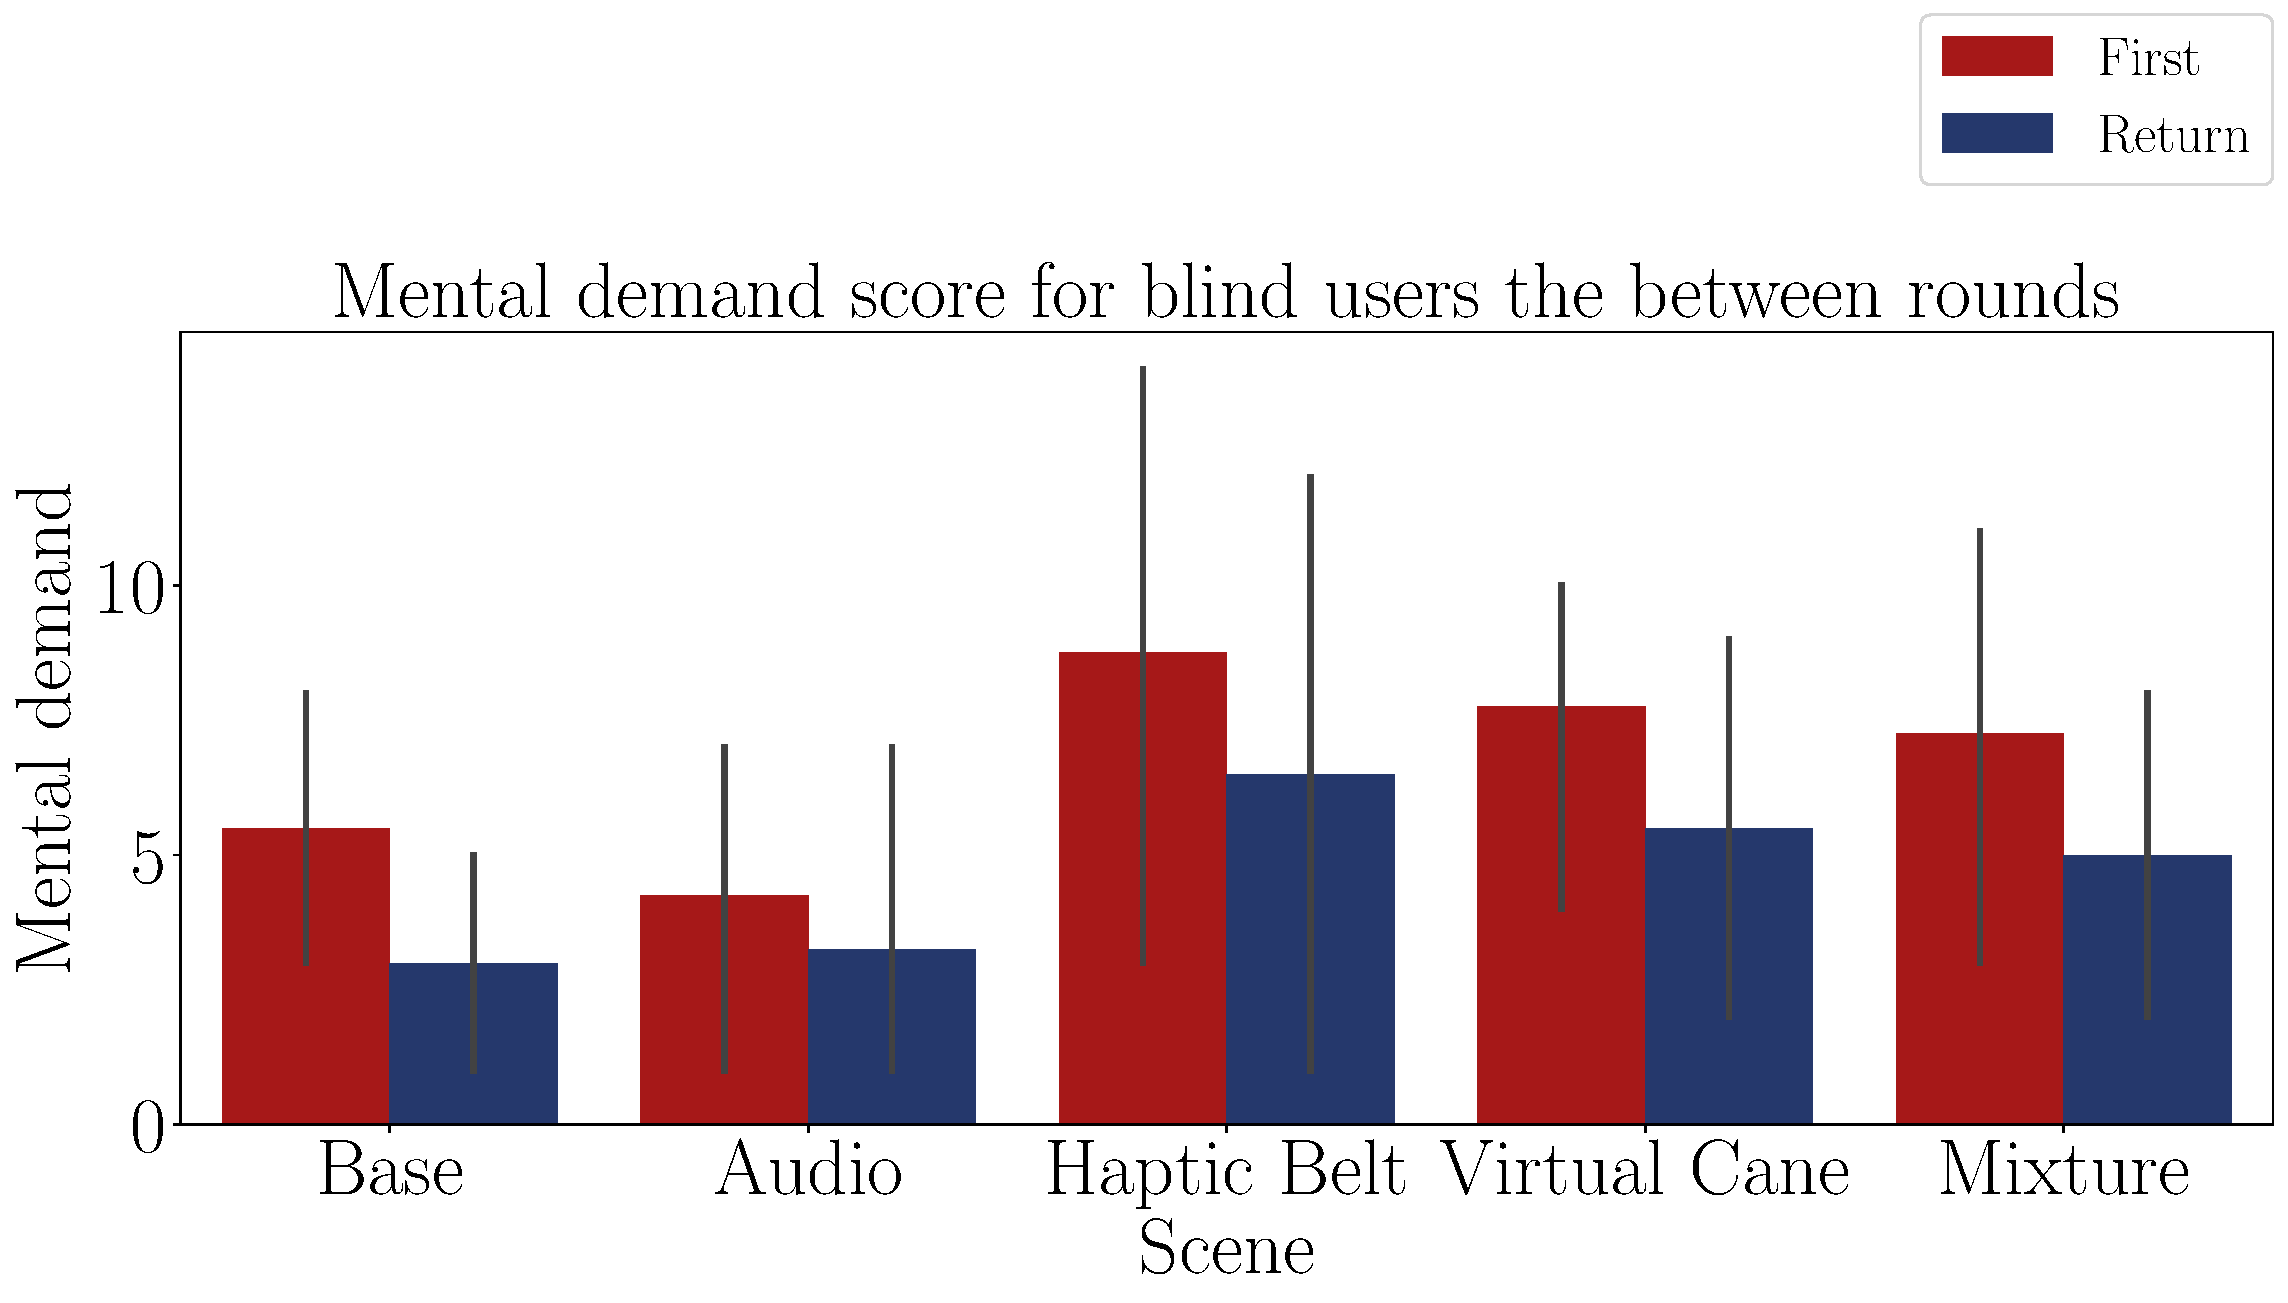
\includegraphics[width = \textwidth]{Resultados/Nasa/Figuras/pdf/barplot_md_avg_5_scene_blind.pdf}
    \caption{Mean and standard deviation of mental demand of blind participants for each method.}
    \label{fig:barplot_md_avg_5_scene_blind}
\end{figure}


Figure \ref{fig:boxplot_md_blind_scene}  presents a boxplot of the mental demand score grouped by the methods. This figure shows that there may be two groups: one associated with lower demand, composed of "base" and "audio", and another with higher demand, composed of "haptic belt", "virtual cane" and "mixture". It indicates that maybe a guidance method that uses vibration as input is not intuitive. Figure \ref{fig:boxplot_md_blind_rounds} presents a boxplot of the mental demand grouped by the rounds, confirming the general tendency to reduce the required "mental demand". 

\begin{figure}[!htb]
    \centering
    \begin{minipage}{0.45\textwidth}
        \centering
        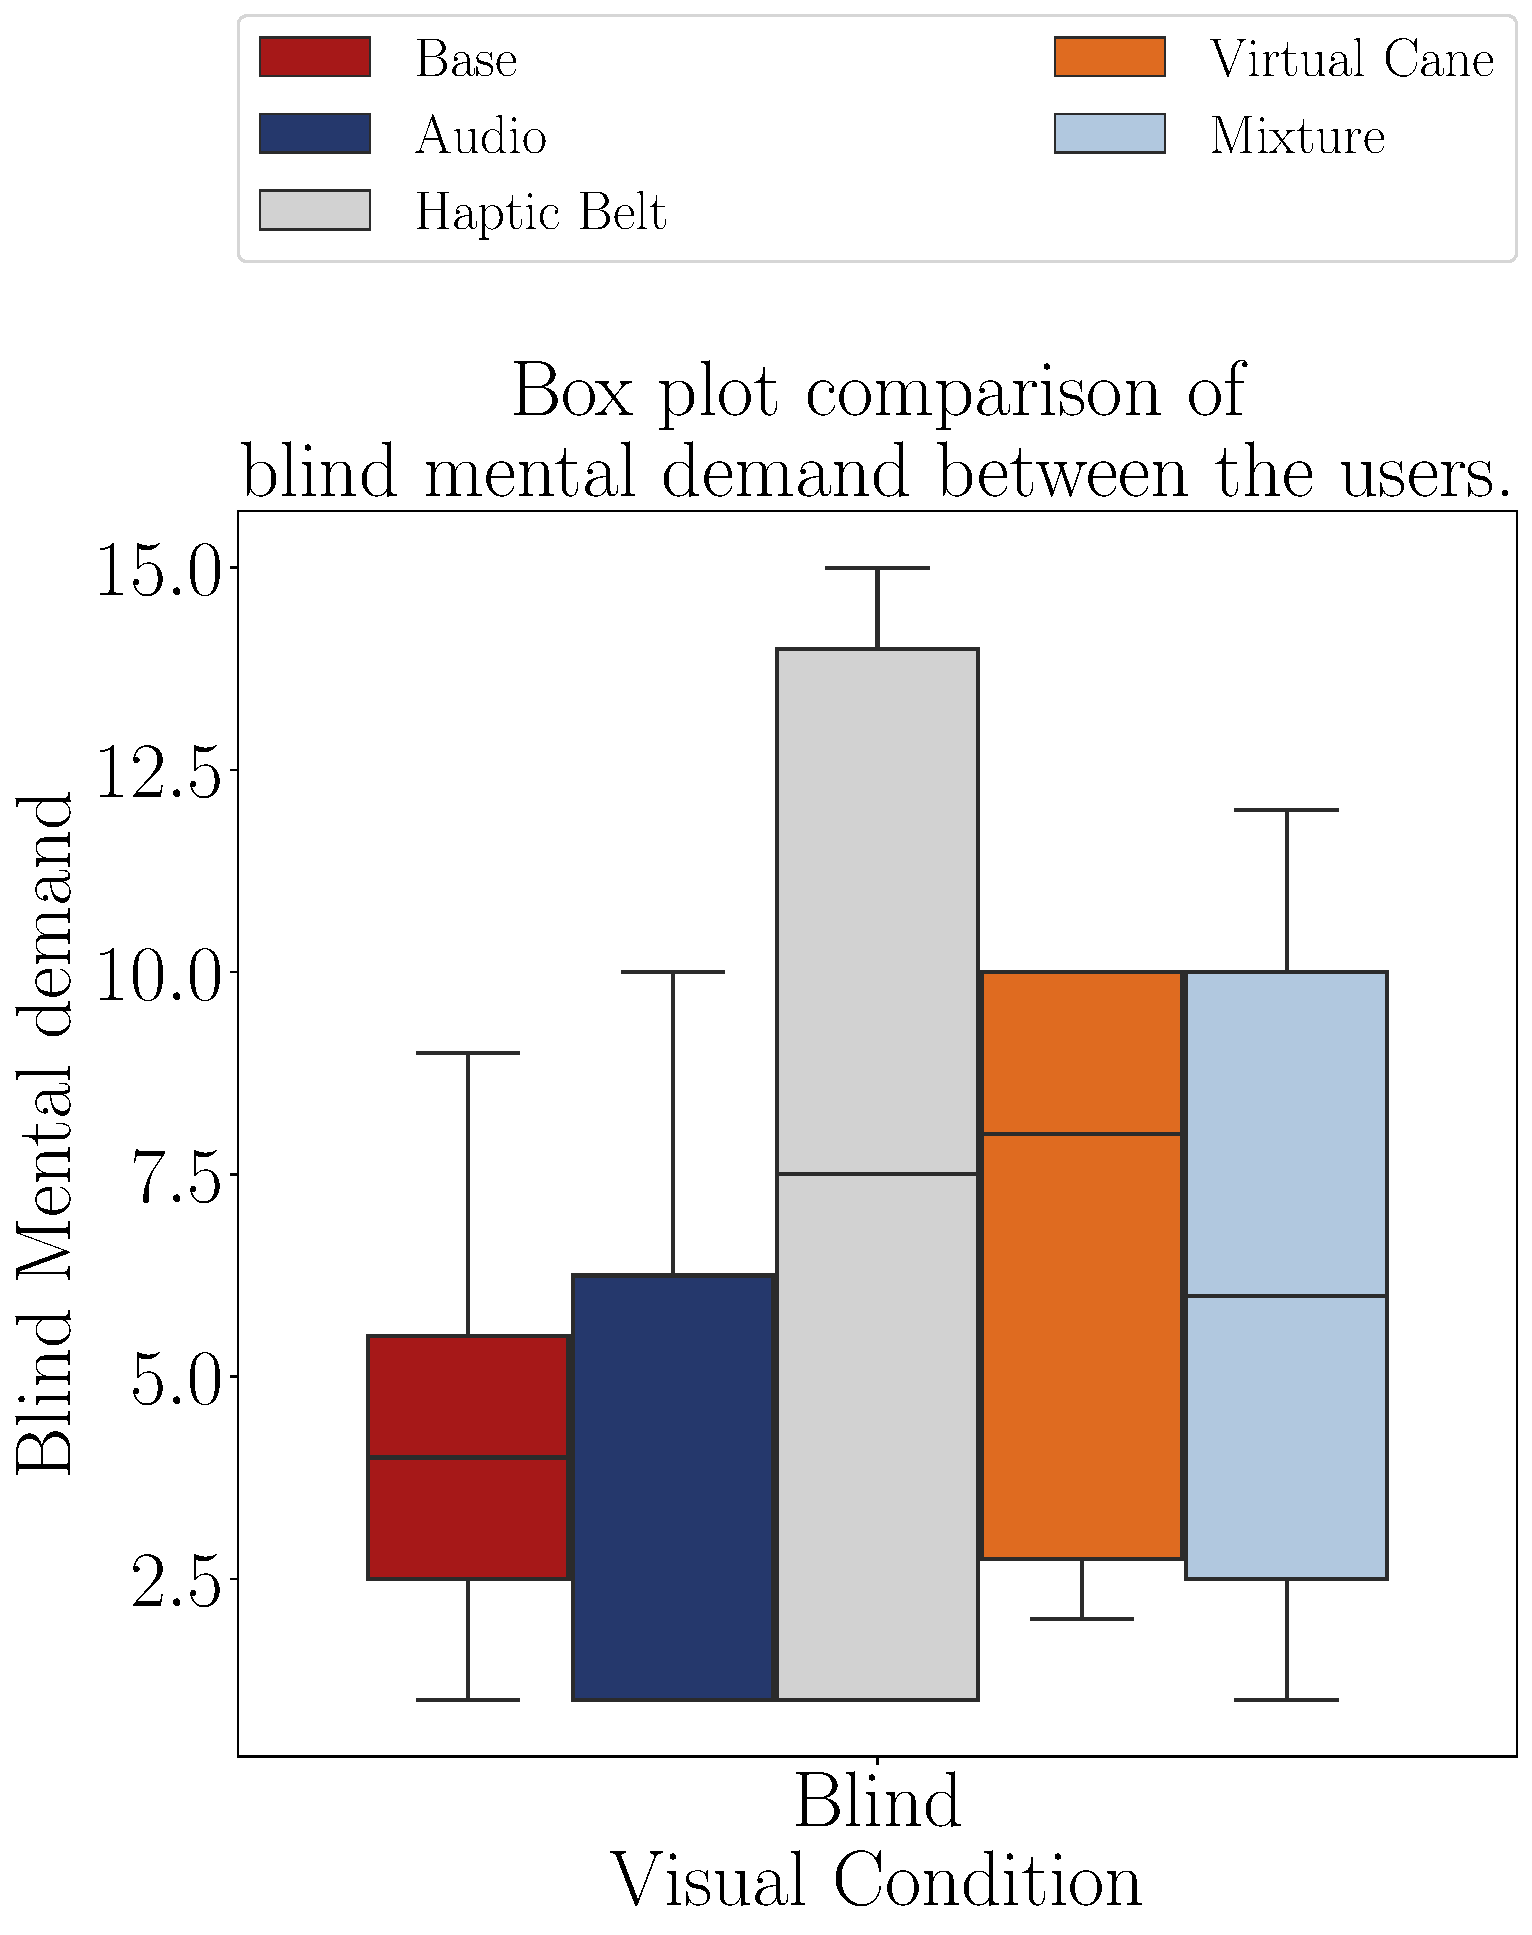
\includegraphics[width = \textwidth]{Resultados/Nasa/Figuras/pdf/boxplot_md_blind_scene.pdf}
        \caption{Boxplot of the mental demand of the blind participants grouped by the methods.}
        \label{fig:boxplot_md_blind_scene}
    \end{minipage}
    \begin{minipage}{0.075\textwidth}
        \hfill
    \end{minipage}
    \begin{minipage}{0.45\textwidth}
        \centering
        %\vspace{3ex}
        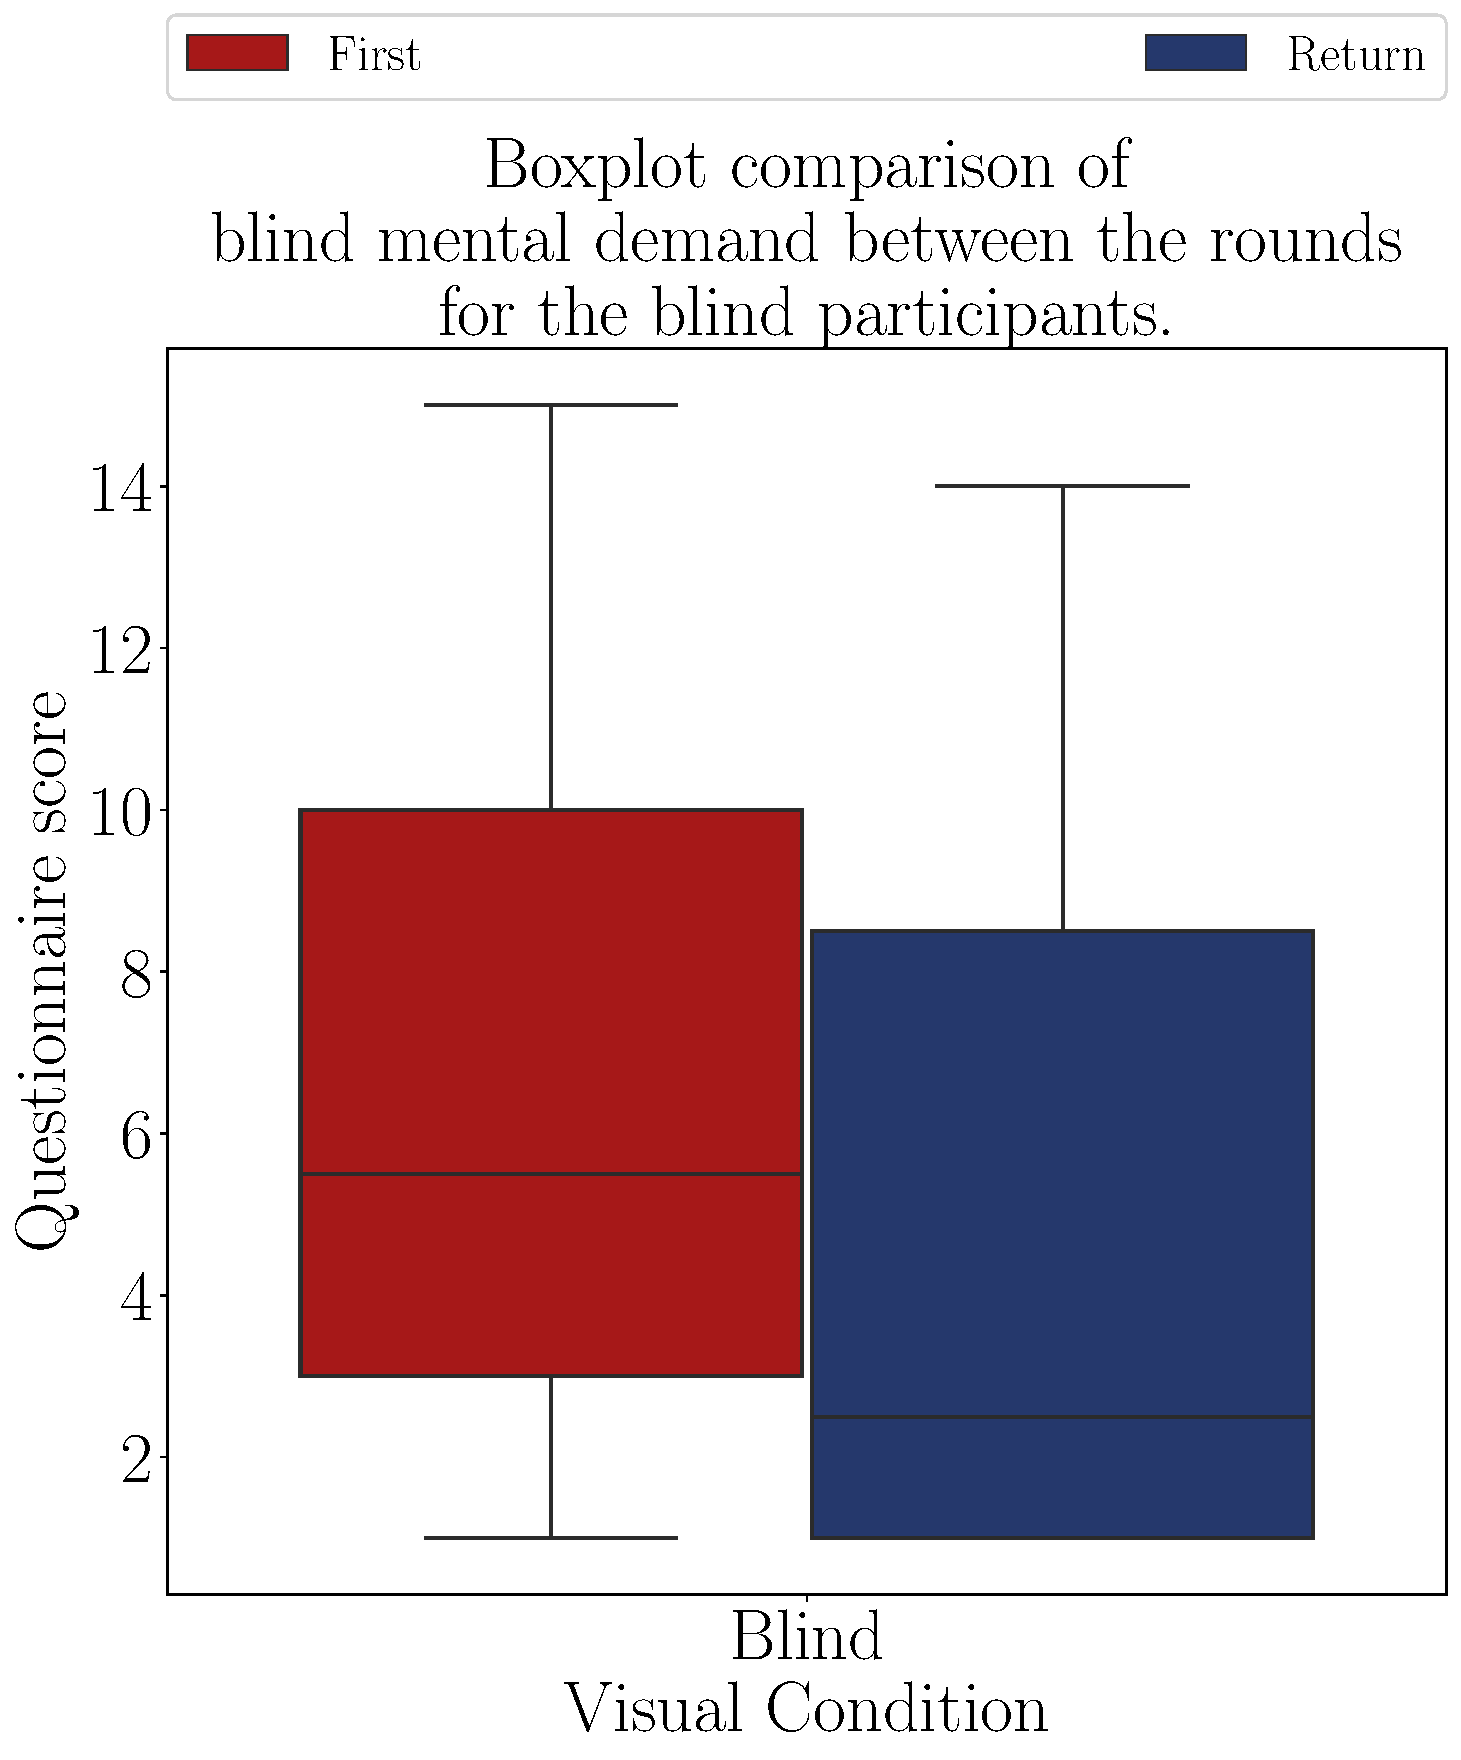
\includegraphics[width = \textwidth]{Resultados/Nasa/Figuras/pdf/boxplot_md_blind_rounds.pdf}
        \caption{Boxplot of the mental demand of the blind participants grouped by the round.}
        \label{fig:boxplot_md_blind_rounds}
    \end{minipage}
\end{figure}

In order to support the statistical analysis, Figures \ref{fig:qqplot_md_avg_two_way_blind} and \ref{fig:residplot_md_avg_two_way_blind} presents the QQ-plot and the residual plot of the "mental demand" data, confirming that the data follow a normal distribution and the residues are homogenous.

Figures \ref{fig:qqplot_md_avg_two_way_blind} and \ref{fig:residplot_md_avg_two_way_blind} show the distribution and variance of Table \ref{tab:md_table_blind}. These figures show that the data are normally distributed and that the methods have a similar variance. Table \ref{tab:blocanova_md_avg_two_way_blind} shows the ANOVA test p-values of the mental demand of the "blind” sample between the guidance methods. The methods' and the rounds' p-values indicate that there is no influence from them in the mental demand. The interaction between the methods and the round also does not influence the mental demand.

\begin{figure}[!htb]
    \centering
    \begin{minipage}{0.45\textwidth}
        \centering
        %\vspace{1ex}
        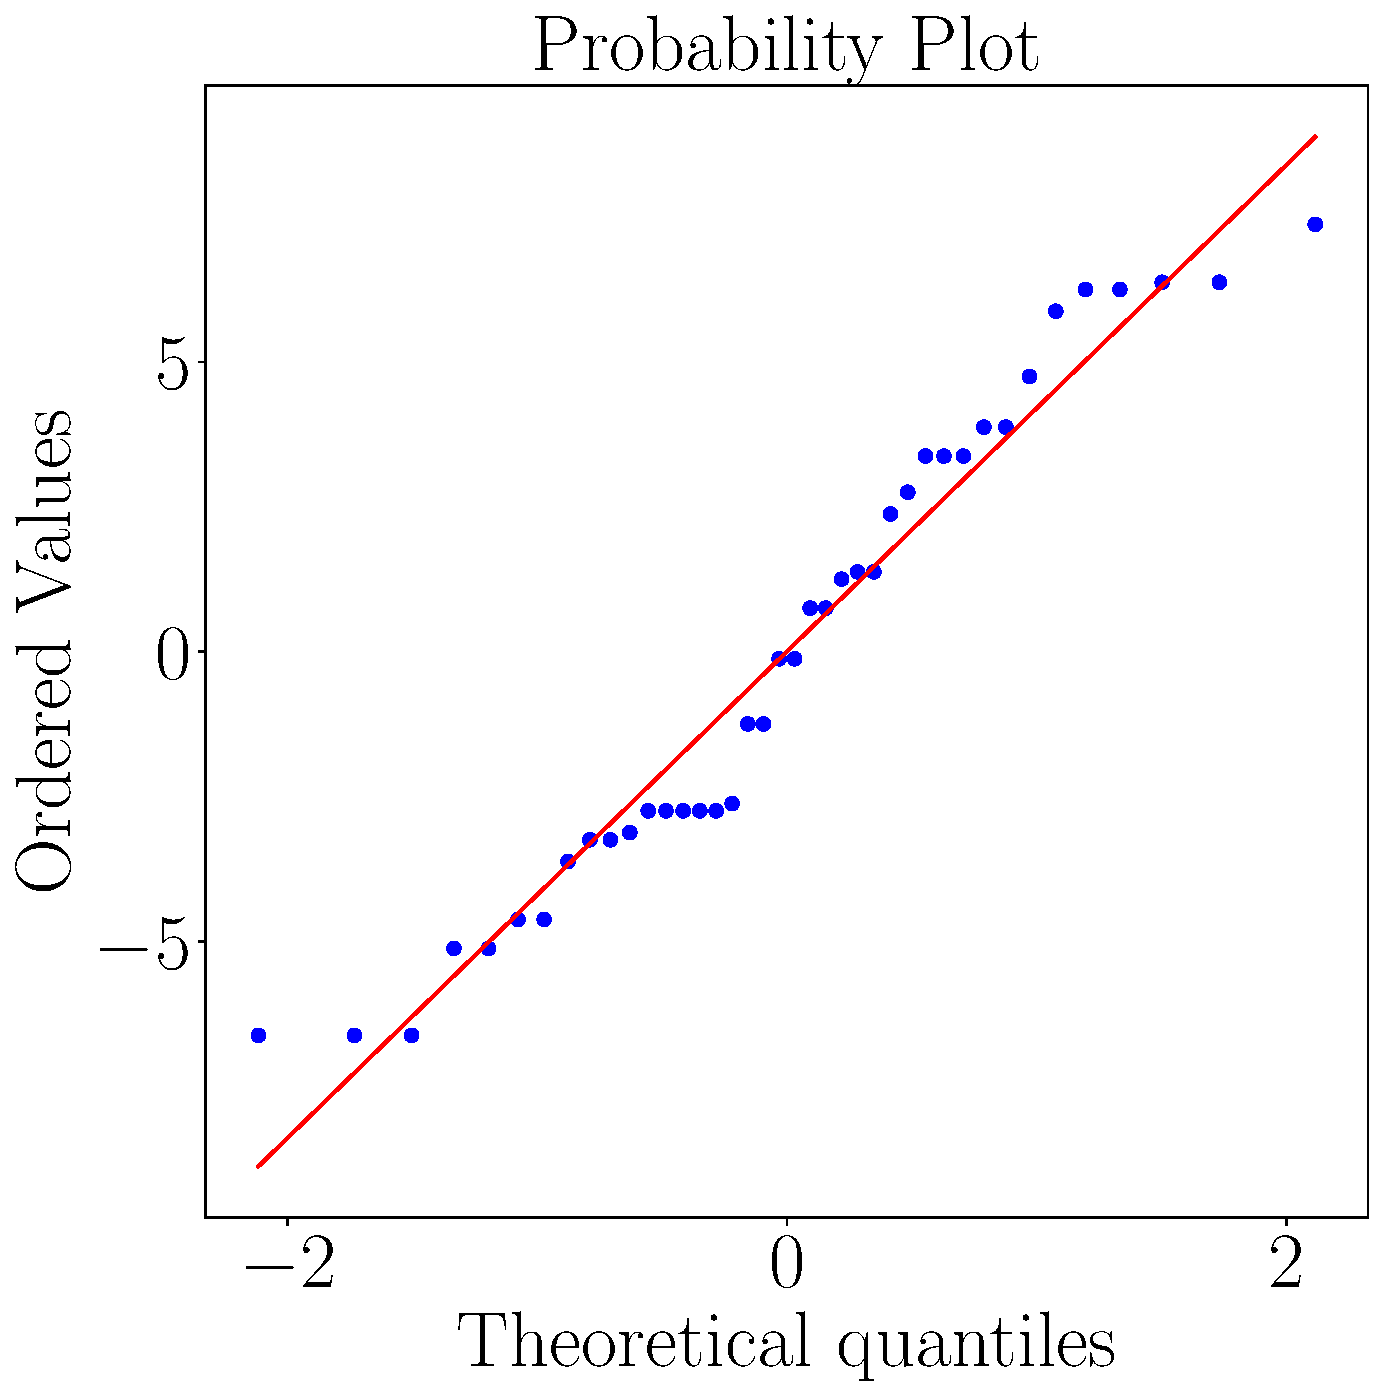
\includegraphics[width = \textwidth]{Resultados/Nasa/Figuras/pdf/qqplot_md_avg_two_way_blind.pdf}
        \caption{QQ plot of the mental demand of the blind participants on each method.}
        \label{fig:qqplot_md_avg_two_way_blind}
    \end{minipage}
    \begin{minipage}{0.075\textwidth}
        \hfill
    \end{minipage}
    \begin{minipage}{0.45\textwidth}
        \centering
        %\vspace{1ex}
        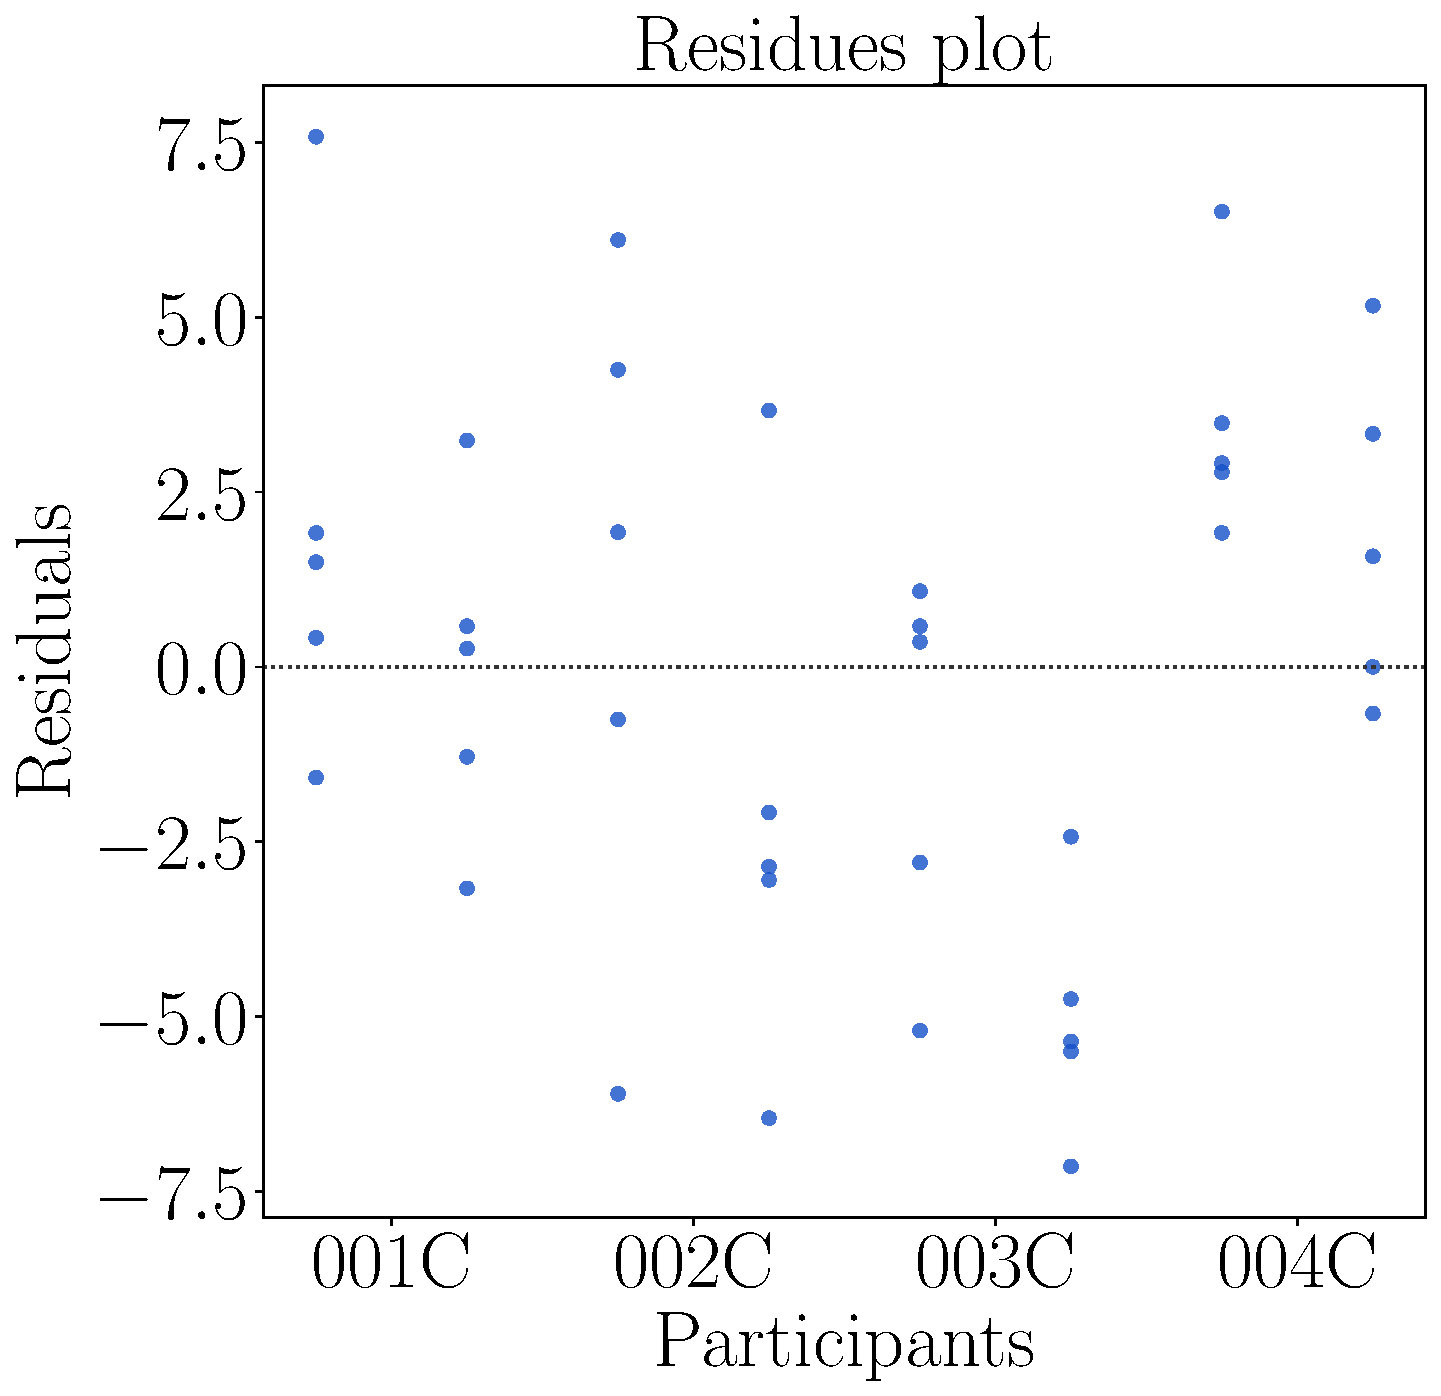
\includegraphics[width = \textwidth]{Resultados/Nasa/Figuras/pdf/residplot_md_avg_two_way_blind.pdf}
        \caption{Residual plot of the mental demand score the blind participants on each method.}
        \label{fig:residplot_md_avg_two_way_blind}
    \end{minipage}
\end{figure}

Following, the statistical model of Equation 5.1 is used for the analysis of variance (ANOVA): 

\begin{equation}
    \label{eq:statistical_model}
    y_{ijk} = \mu + \tau_i + \beta_j + \msout{\omega_k} + (\tau\beta_{ij}) + e
\end{equation}

where:

\begin{itemize}
    \item $y_{ij}$ - output variable for method $i$, round $j$ and participant $k$;
    \item $\mu$ - mean of all the observations;
    \item $\tau_i$ - variance from method $i$;
    \item $\beta_j$ - variance from round $j$;
    \item \sout{$\omega_k$} - variance from participant k, which is treated as a block;
    \item $\tau\beta_{ij}$ - combined variance from the interaction between method i and round j;
    \item $e$ - residual error.
\end{itemize}

The results of ANOVA are presented in Table \ref{tab:blocanova_md_avg_two_way_blind}. ANOVA tests the hypothesis that the means of independent data groups are equal or not. In the literature, a p-value of 0.05 is commonly adopted as a threshold to confirm the hypothesis. A p-value < 0.05 indicates that the means of the groups are statistically different with 95\% of confidence. According to this criterion, neither method or round have a significant influence on the mental demand.

However, due to the low number of participants, the threshold of 0.1 could also be considered. In this case, it indicates, with 90\% confidence, that the mean of the "first" and "return" rounds are different. For the guidance method, the p-value of 0.170 is close to the threshold but slightly higher, suggesting that the means may be different. However, this hypothesis is not statistically confirmed with the current data. 


\begin{table}[!htb]
\centering
\caption{Anova p-value for the mental demand average on each method for blinded users.}
\label{tab:blocanova_md_avg_two_way_blind}
\begin{tabular}{lrrrrl}
\toprule
               Source &  Squared sum &  DOF & Squared average &     F & \begin{tabular}[c]{@{}l@{}}P-Value \\ $(F_{0} > F)$\end{tabular} \\
\midrule
Participants (Blocks) &      298.475 &    3 &          99.492 & 8.133 &                                                                  \\
         \    Methods &       85.150 &    4 &          21.288 & 1.740 &                                                            0.170 \\
          \    Rounds &       42.025 &    1 &          42.025 & 3.436 &                                                            0.075 \\
     \    Interaction &        2.850 &    4 &           0.712 & 0.058 &                                                            0.993 \\
   Experimental Error &      330.275 &   27 &          12.232 &       &                                                                  \\
                Total &      758.775 &   39 &                 &       &                                                                  \\
\bottomrule
\end{tabular}
\end{table}



In order to conclude the analysis of the NASA-TLX mental demand, Table \ref{tab:md_var_average_group_blind} brings the average difference between the mental demand of the "first" and "return" rounds. Unexpectedly, it shows that the most significant variation is obtained to the "base", i.e., the guidance method the participant uses and, therefore, should not present a significant variation. The methods with the lower variation was "audio", probably because it already had a shallow score in the first round. 


\begin{table}[!htb]
\centering
\caption{Mental demand variation grouped by participant and visual condition}
\label{tab:md_var_average_group_blind}
\begin{tabular}{lrrrrrr}
\toprule
{} &  Base & Audio & \begin{tabular}[c]{@{}l@{}}Haptic\\ Belt\end{tabular} & \begin{tabular}[c]{@{}l@{}}Virtual\\ Cane\end{tabular} & Mixture \\
Visual Condition &       &       &                                                       &                                                        &         \\
\midrule
Blind            &  -2.5 &  -1.0 &                                                  -2.2 &                                                   -2.2 &    -2.2 \\
\bottomrule
\end{tabular}
\end{table}



\FloatBarrier

%%%%%%%%%%%%%%%%%%%%%%%%%%%%%%%%%%%%%%%%%%%%%%%%%%%%%%%%%%%%%%%%%%%%%%%%%%%
%%%%%%%%%%%%%%%%%%%%%%%%%%%%%%%%%%%%%%%%%%%%%%%%%%%%%%%%%%%%%%%%%%%%%%%%%%%
%%%%%%%%%%%%%%%%%%%%%%%%%%%%%%%%%%%%%%%%%%%%%%%%%%%%%%%%%%%%%%%%%%%%%%%%%%%
%%%%%%%%%%%%%%%%%%%%%%%%%%%%%%%%%%%%%%%%%%%%%%%%%%%%%%%%%%%%%%%%%%%%%%%%%%%


\paragraph{Analysis of the NASA-TLX score}\mbox{}\\

This section repeats the analysis steps of the previous section but now considers the mean value of all dimensions of NASA-TLX, referred to in this text as the global score. Table \ref{tab:nasa_table_blind} presents the global score of each blind participant. 


\begin{table}[!htb]
\centering
\caption{NASA-TLX score felled by the blinded participants.}
\label{tab:nasa_table_blind}
\begin{tabular}{llrrrrr}
\toprule
     &        &  Base &  Audio & \begin{tabular}[c]{@{}l@{}}Haptic\\ Belt\end{tabular} & \begin{tabular}[c]{@{}l@{}}Virtual\\ Cane\end{tabular} & Mixture \\
Participant & Round &       &        &                                                       &                                                        &         \\
\midrule
001C & First & 4.833 &  4.000 &                                                 8.833 &                                                  5.167 &   6.333 \\
     & Return & 4.167 &  4.000 &                                                 6.667 &                                                  4.500 &   6.167 \\
002C & First & 6.333 &  4.833 &                                                 4.833 &                                                  9.000 &   7.000 \\
     & Return & 4.500 &  4.833 &                                                 4.833 &                                                  7.000 &   5.167 \\
003C & First & 4.000 &  4.000 &                                                 5.333 &                                                  6.667 &   3.500 \\
     & Return & 4.000 &  3.833 &                                                 3.667 &                                                  3.500 &   3.500 \\
004C & First & 9.833 & 10.000 &                                                12.667 &                                                  9.667 &  11.000 \\
     & Return & 8.667 &  9.167 &                                                11.667 &                                                  9.333 &  10.833 \\
\bottomrule
\end{tabular}
\end{table}



Figure \ref{fig:barplot_nasa_avg_5_scene_blind} brings the corresponding barplot with the mean value and standard deviation for each guidance method and each round. In a qualitative comparison with Figure \ref{fig:barplot_md_avg_5_scene_blind}, the differences between the methods are confirmed but softened. It is possible to notice that the mean score of "audio" and "base" are still lower than that of the other methods. The differences between "first" and "return" rounds are also reduced. However, the standard deviation is also considerably reduced for all methods, and especially for the haptic belt.

\begin{figure}[!htb]
    \centering
    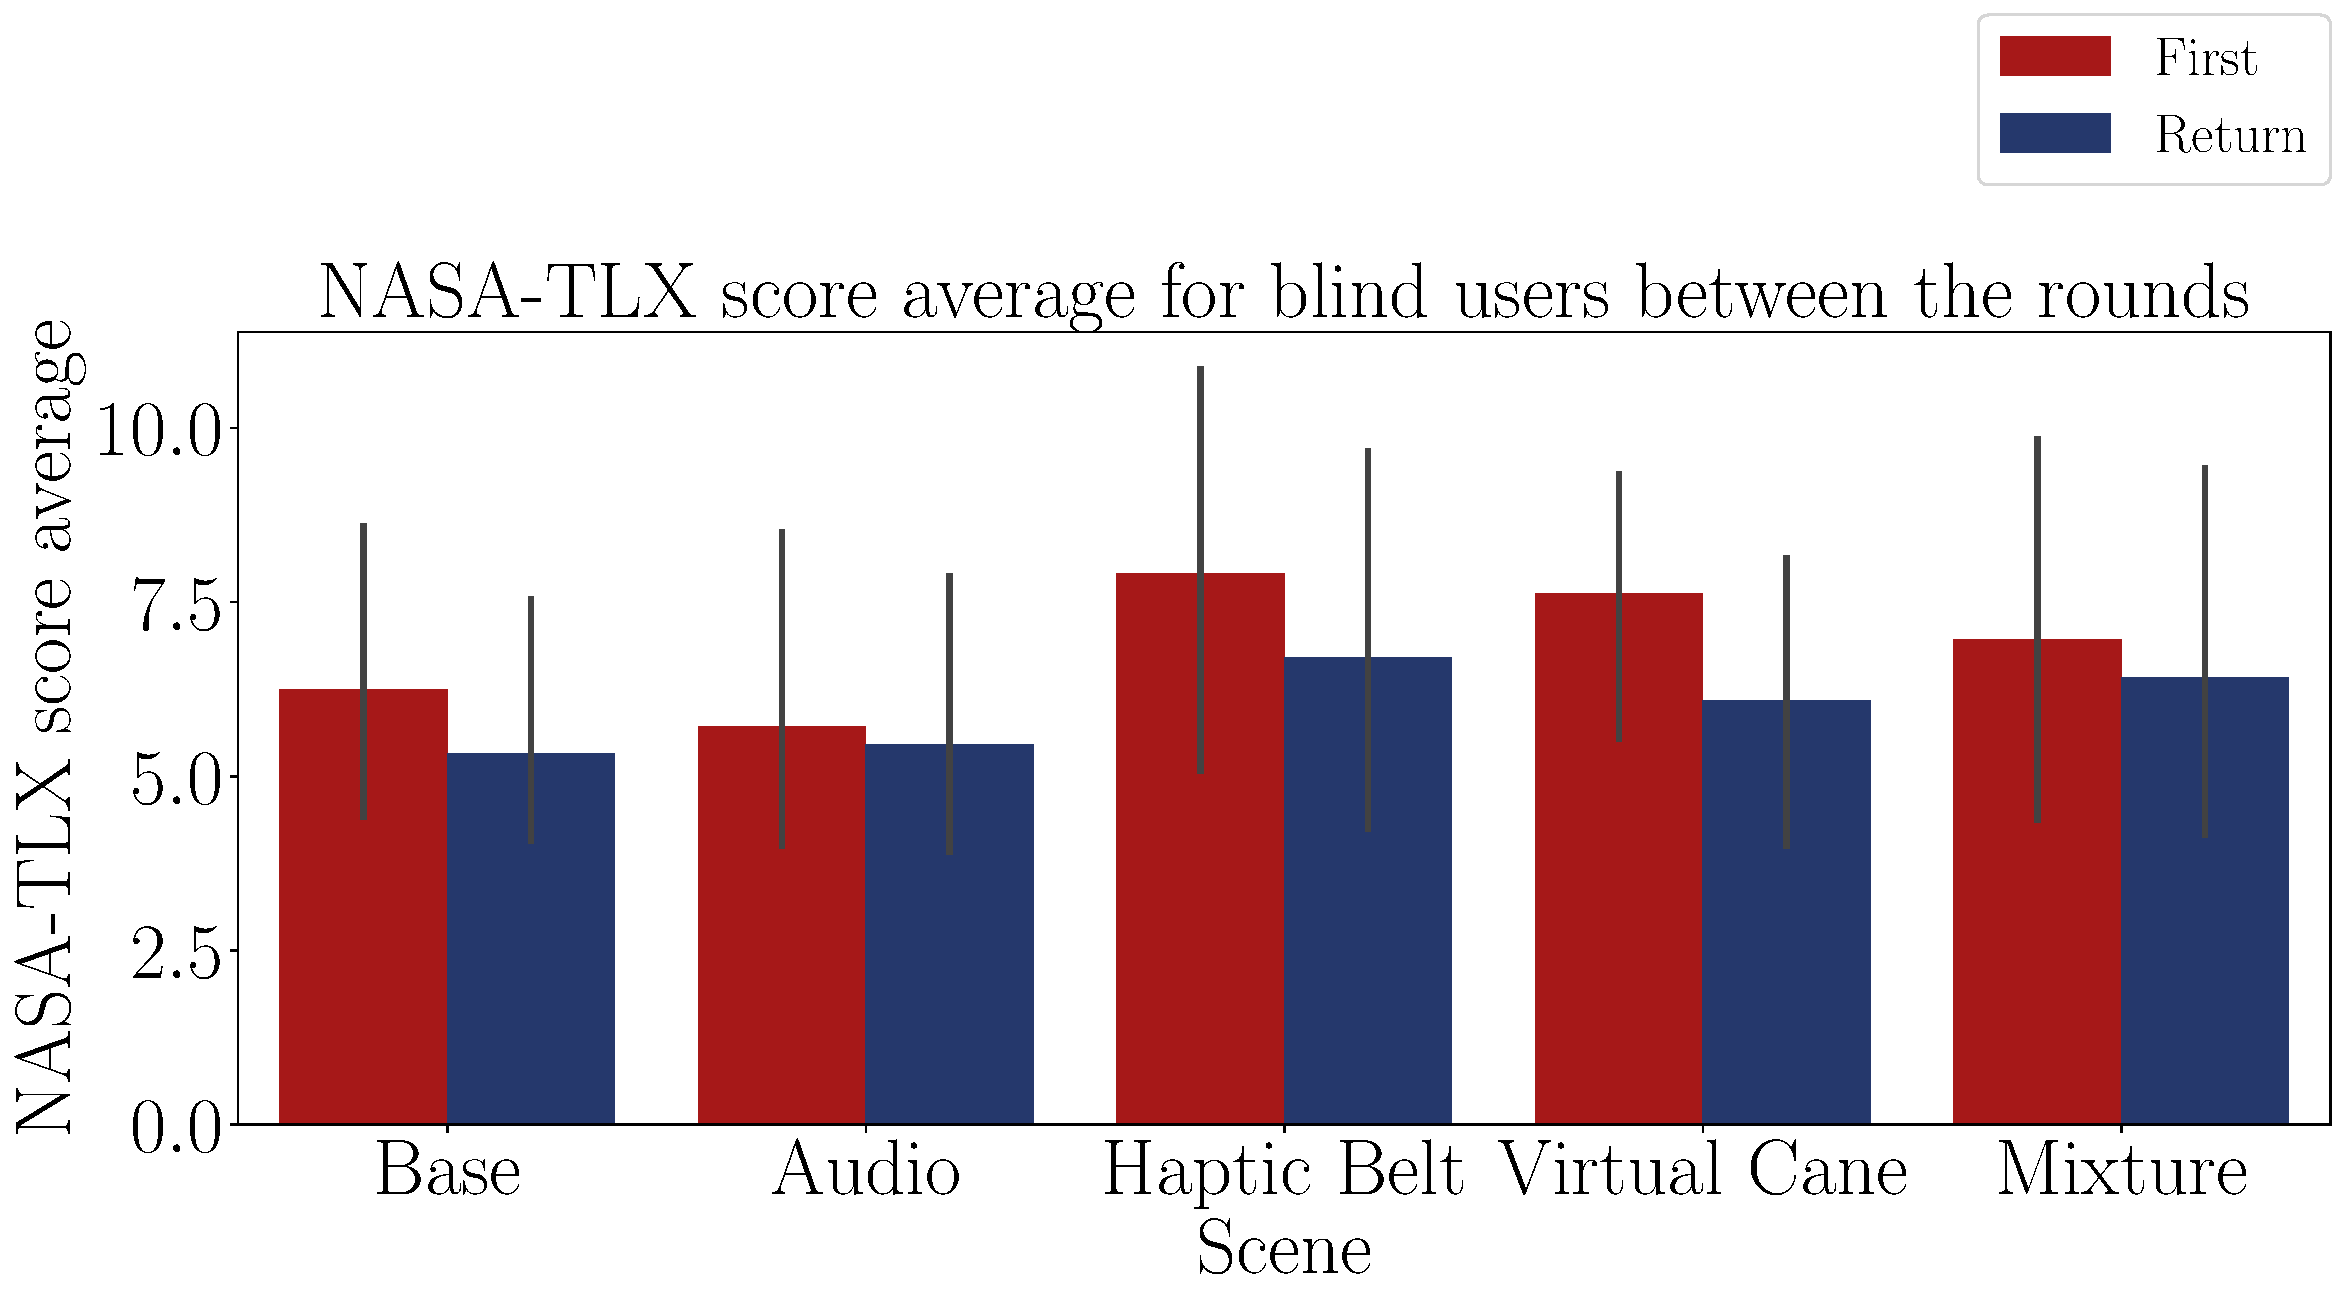
\includegraphics[width = \textwidth]{Resultados/Nasa/Figuras/pdf/barplot_nasa_avg_5_scene_blind.pdf}
    \caption{Barplot of the average NASA-TLX score of the blind participants on each method.}
    \label{fig:barplot_nasa_avg_5_scene_blind}
\end{figure}

Figure \ref{fig:boxplot_nasa_blind_scene} presents the boxplot with the NASA-TLX global score grouped by the methods. Similar to what happened for the "mental demand", it is possible to split the methods into two different groups: "base" and "audio", which require a lower level of workload, and another group, which requires a higher level. Figure \ref{fig:boxplot_nasa_blind_rounds} presents a boxplot with the NASA-TLX global score grouped by the rounds, showing that the two groups are still different. 

\begin{figure}[!htb]
    \centering
    \begin{minipage}{0.45\textwidth}
        \centering
        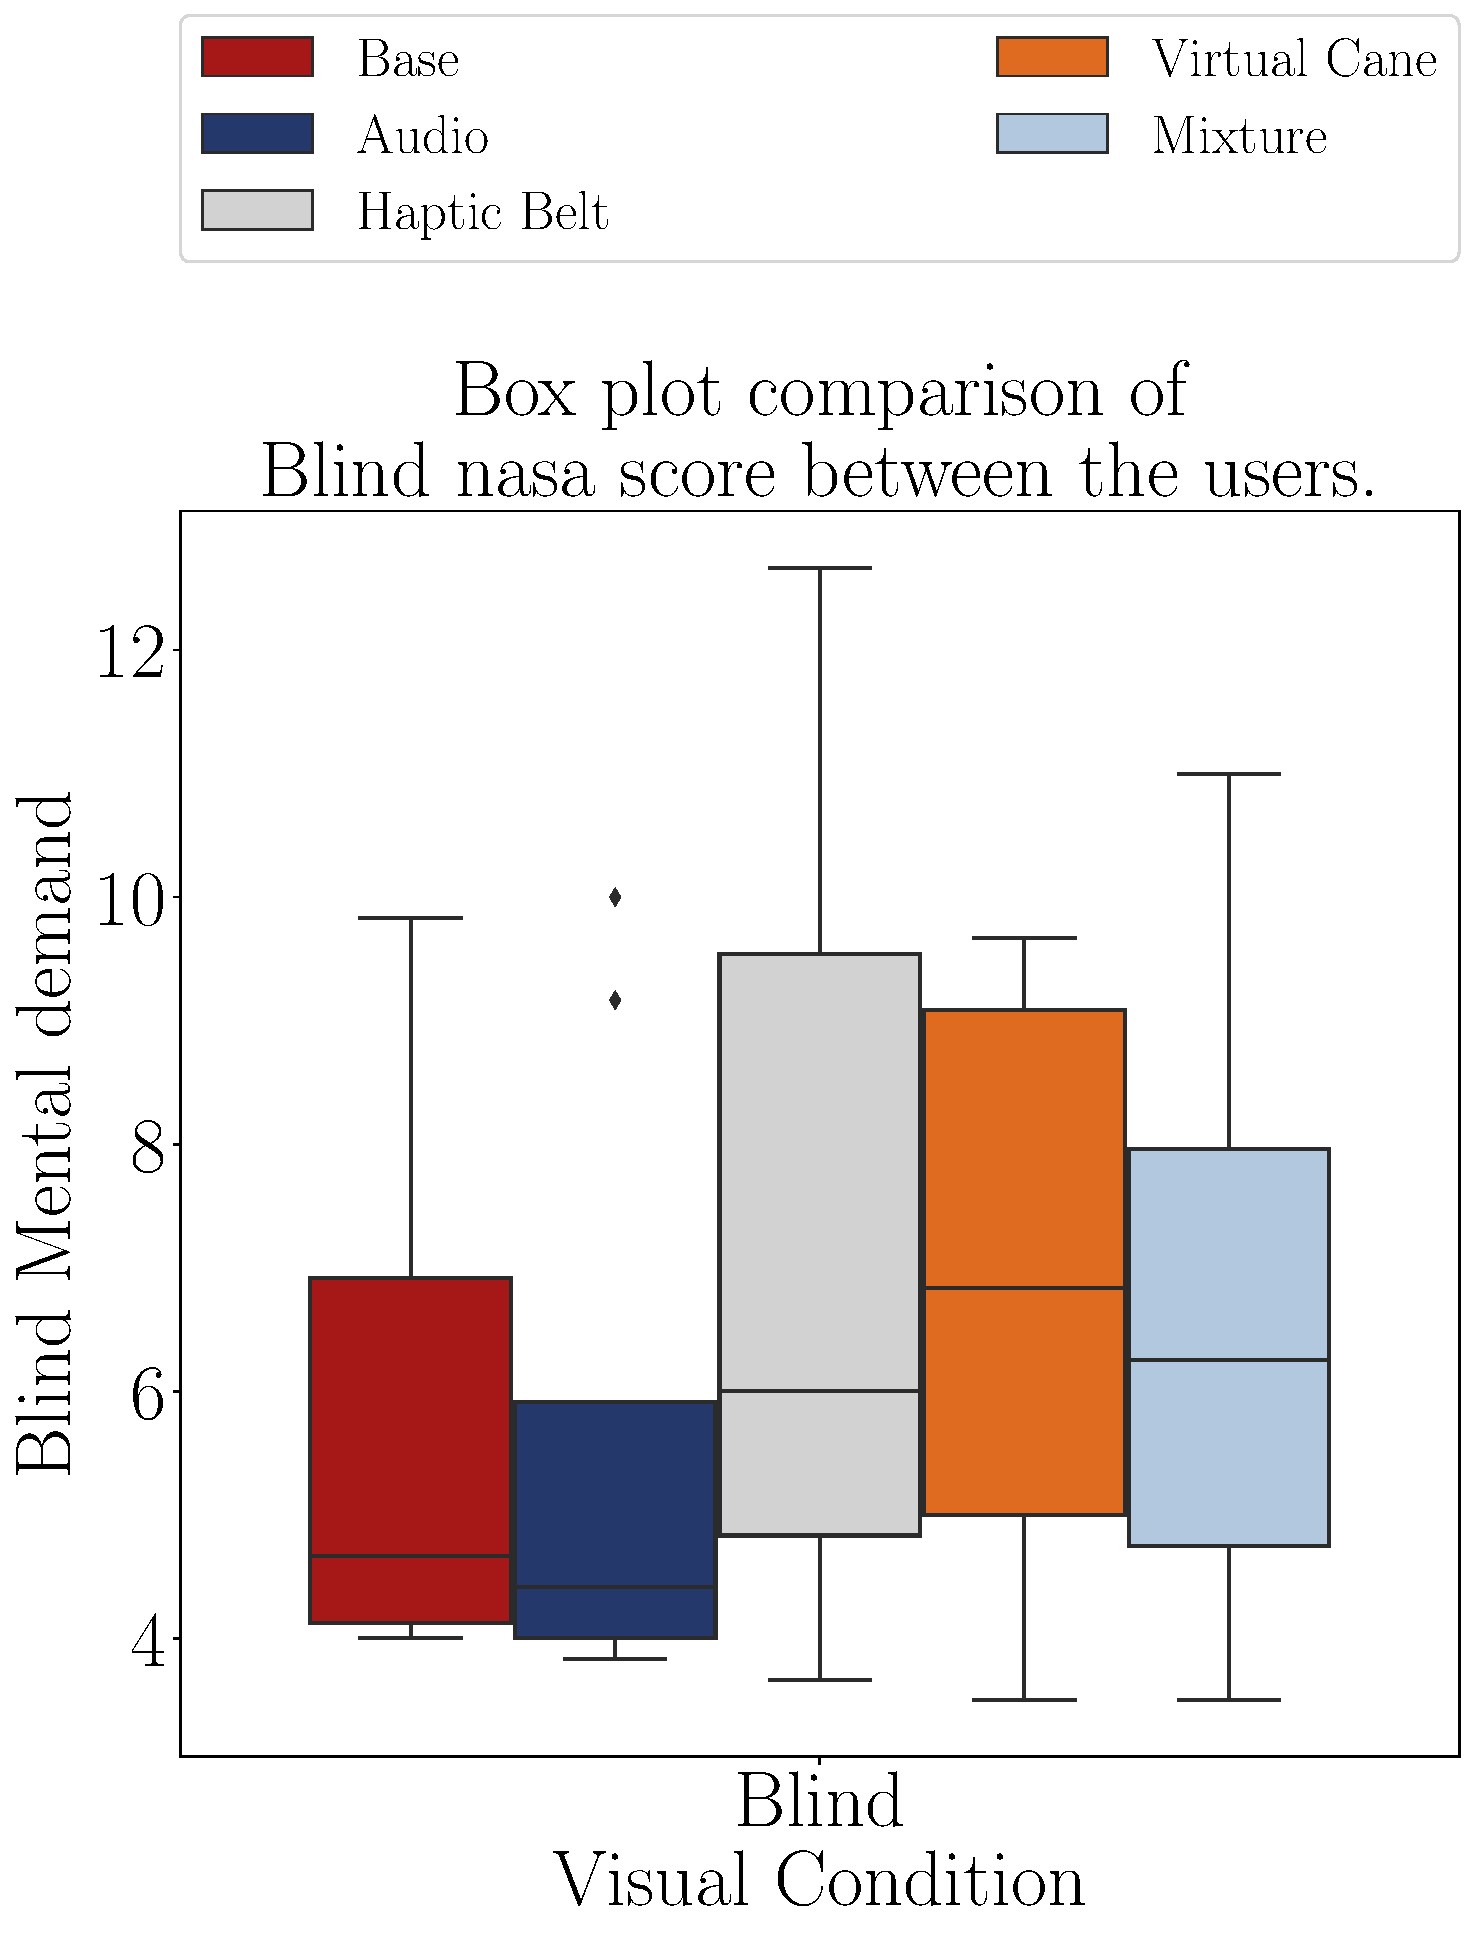
\includegraphics[width = \textwidth]{Resultados/Nasa/Figuras/pdf/boxplot_nasa_blind_scene.pdf}
        \caption{Boxplot of the NASA-TLX of the blind participants grouped by the methods.}
        \label{fig:boxplot_nasa_blind_scene}
    \end{minipage}
    \begin{minipage}{0.075\textwidth}
        \hfill
    \end{minipage}
    \begin{minipage}{0.45\textwidth}
        \centering
        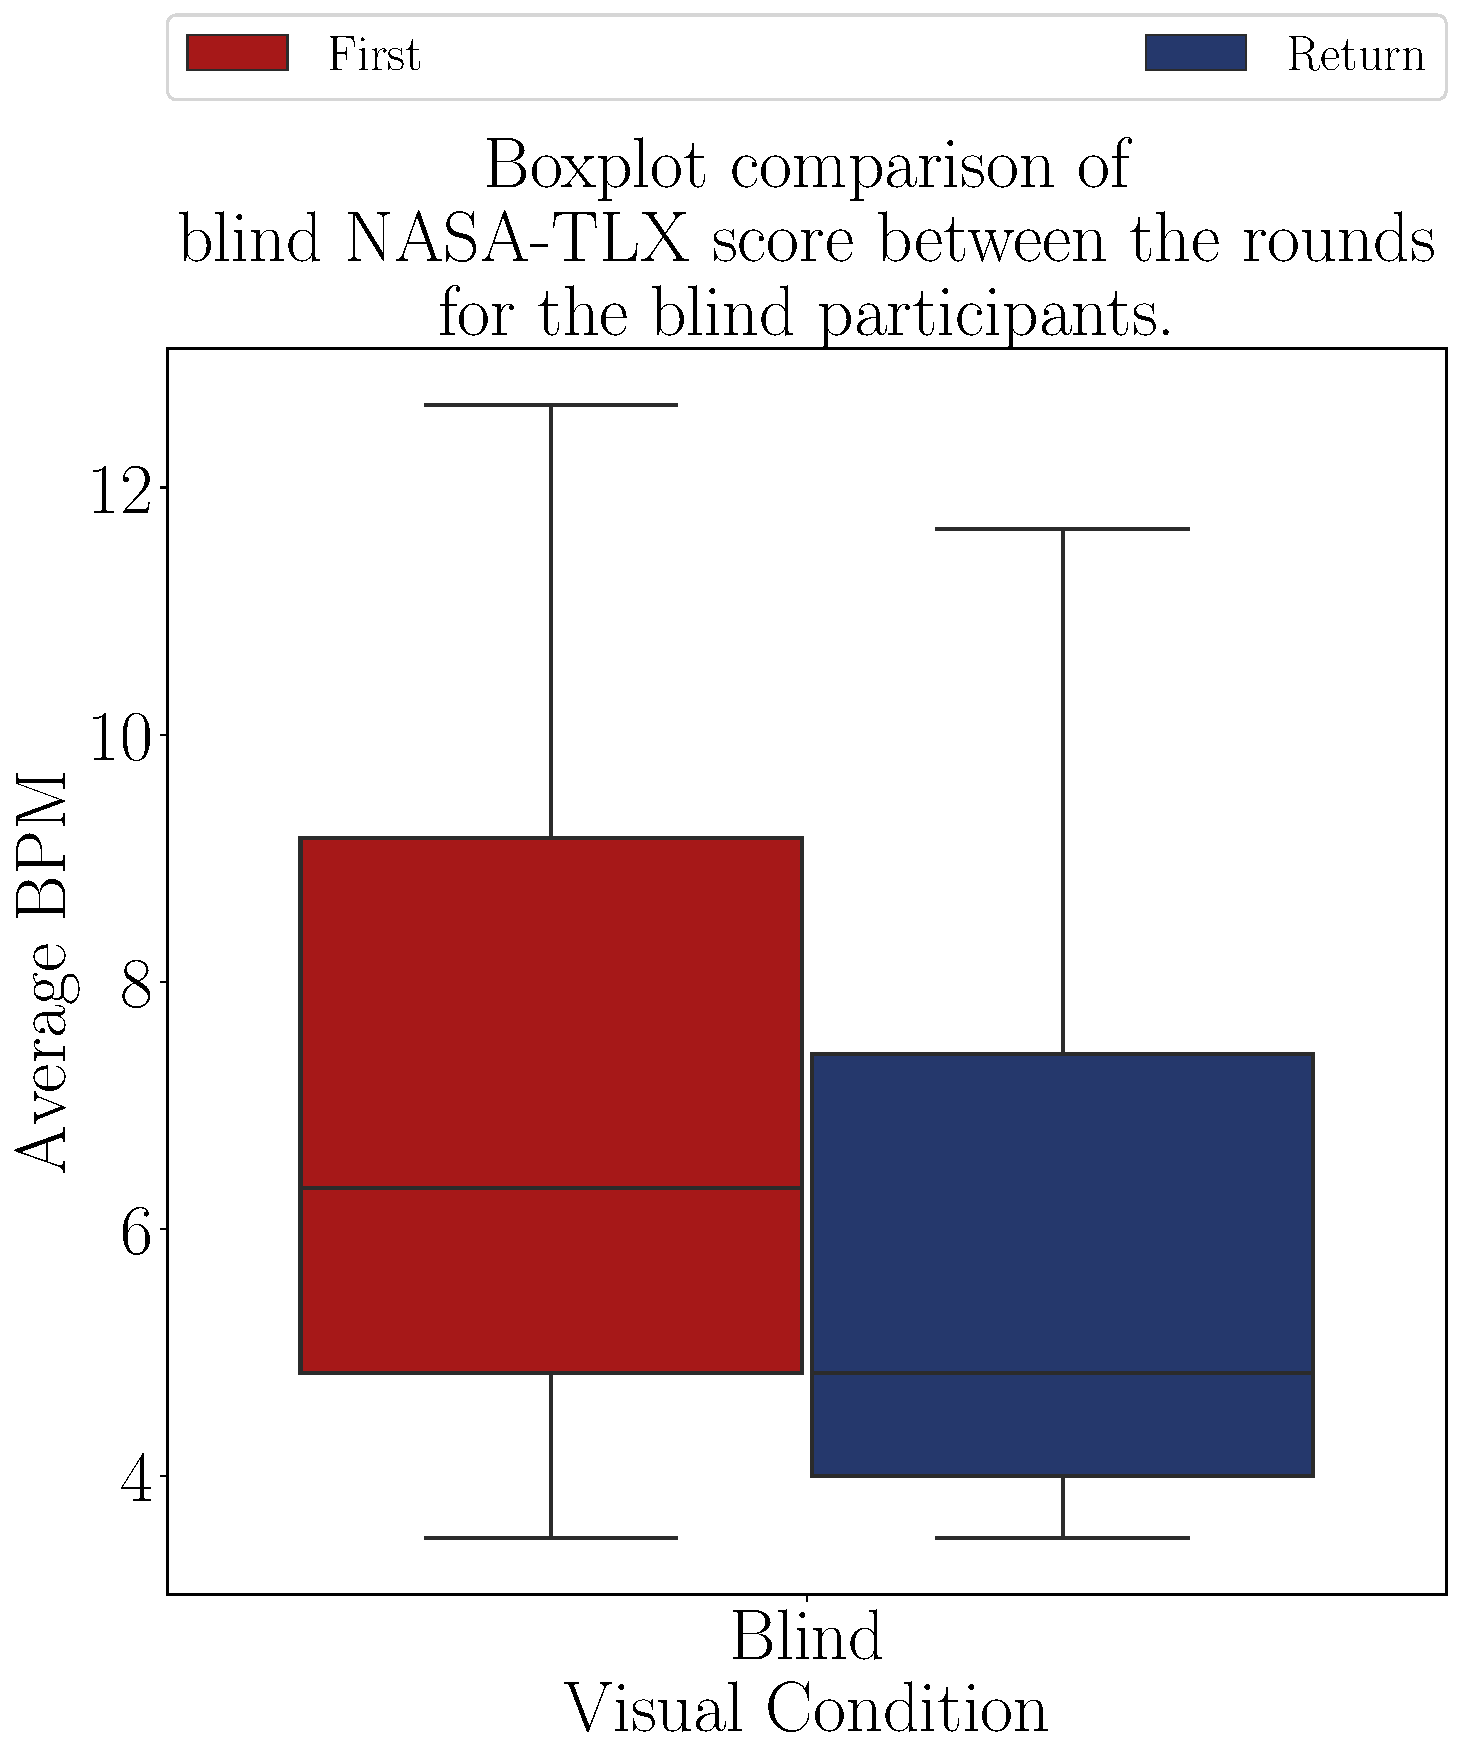
\includegraphics[width = \textwidth]{Resultados/Nasa/Figuras/pdf/boxplot_nasa_blind_rounds.pdf}
        \caption{Boxplot of the NASA-TLX demand of the blind participants grouped by the round.}
        \label{fig:boxplot_nasa_blind_rounds}
    \end{minipage}
\end{figure}

Figures \ref{fig:qqplot_nasa_avg_two_way_blind} and \ref{fig:residplot_nasa_avg_two_way_blind} presents the QQ plot and residual distribution of the NASA-TLX global score, showing that the data are normally distributed. However, the residuals are not so homogeneous as in the previous case, showing that the participants have different variability among them.

\begin{figure}[!htb]
    \centering
    \begin{minipage}{0.45\textwidth}
        \centering
        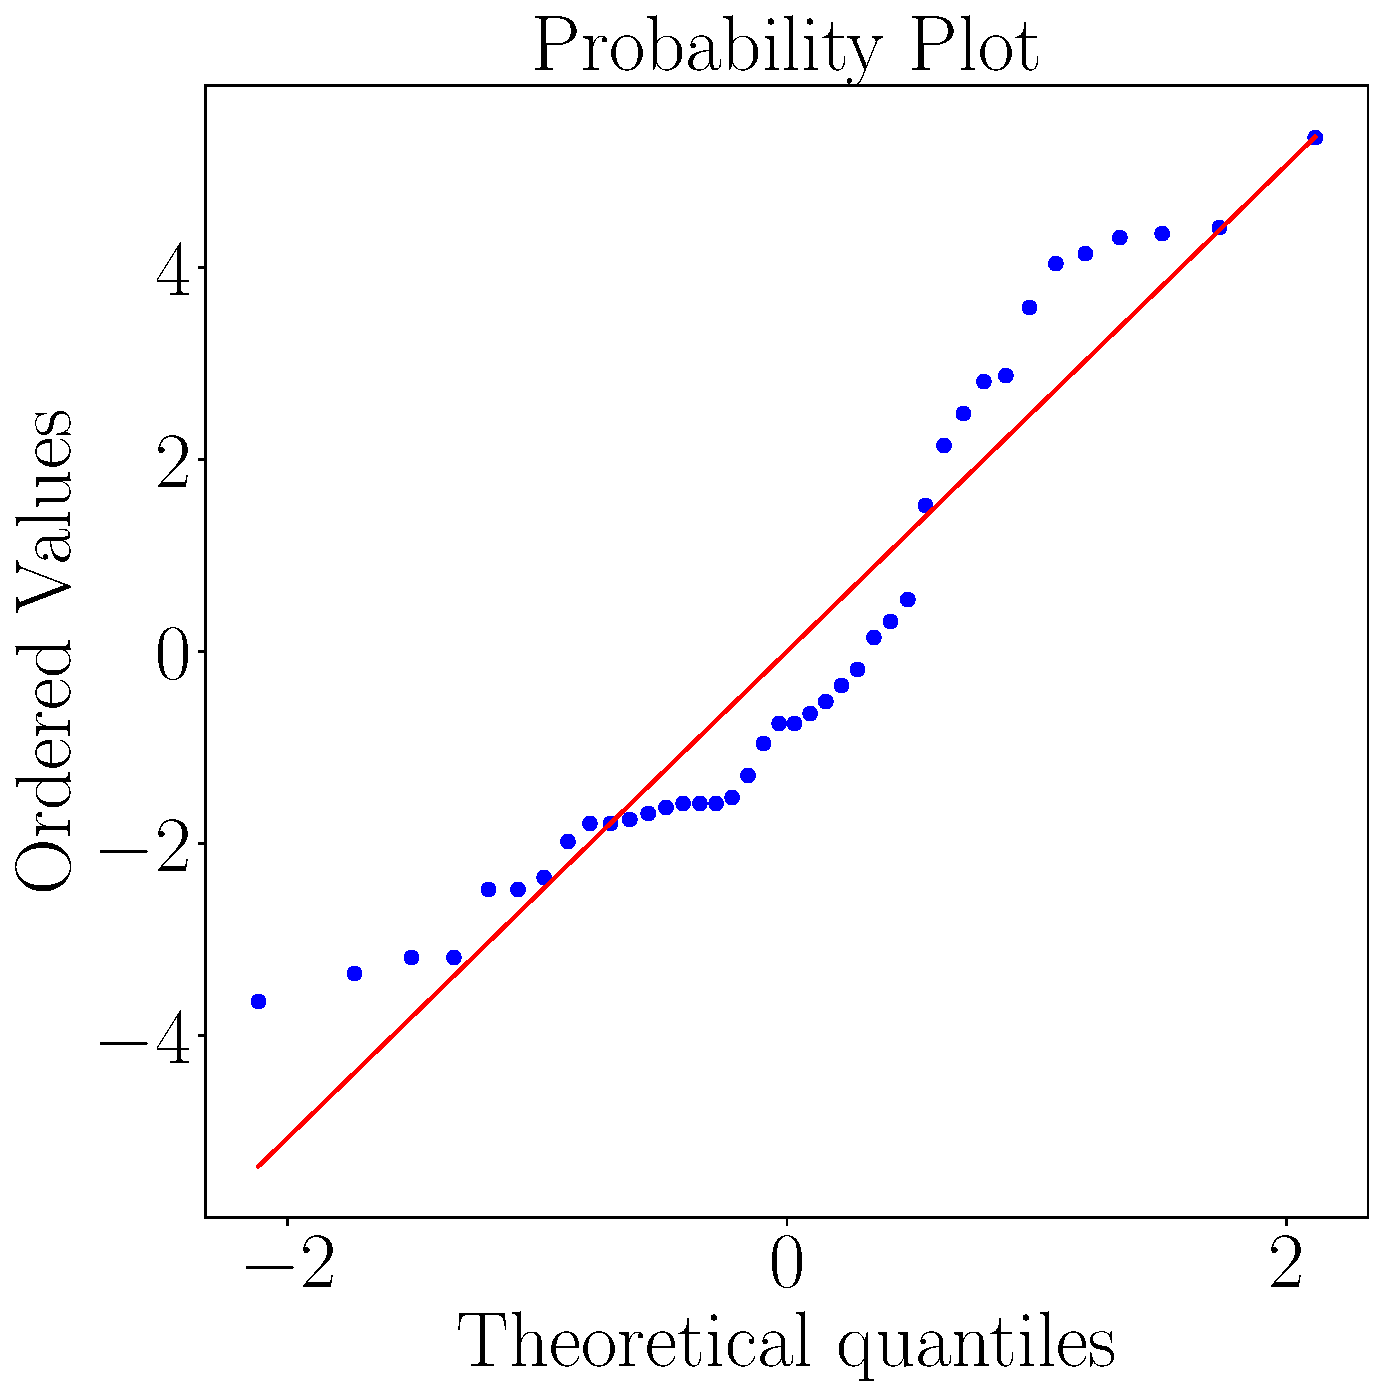
\includegraphics[width = \textwidth]{Resultados/Nasa/Figuras/pdf/qqplot_nasa_avg_two_way_blind.pdf}
        \caption{QQ plot of the NASA-TLX score of the blind participants on each method.}
        \label{fig:qqplot_nasa_avg_two_way_blind}
    \end{minipage}
    \begin{minipage}{0.075\textwidth}
        \hfill
    \end{minipage}
    \begin{minipage}{0.45\textwidth}
        %\vspace{2ex}
        \centering
        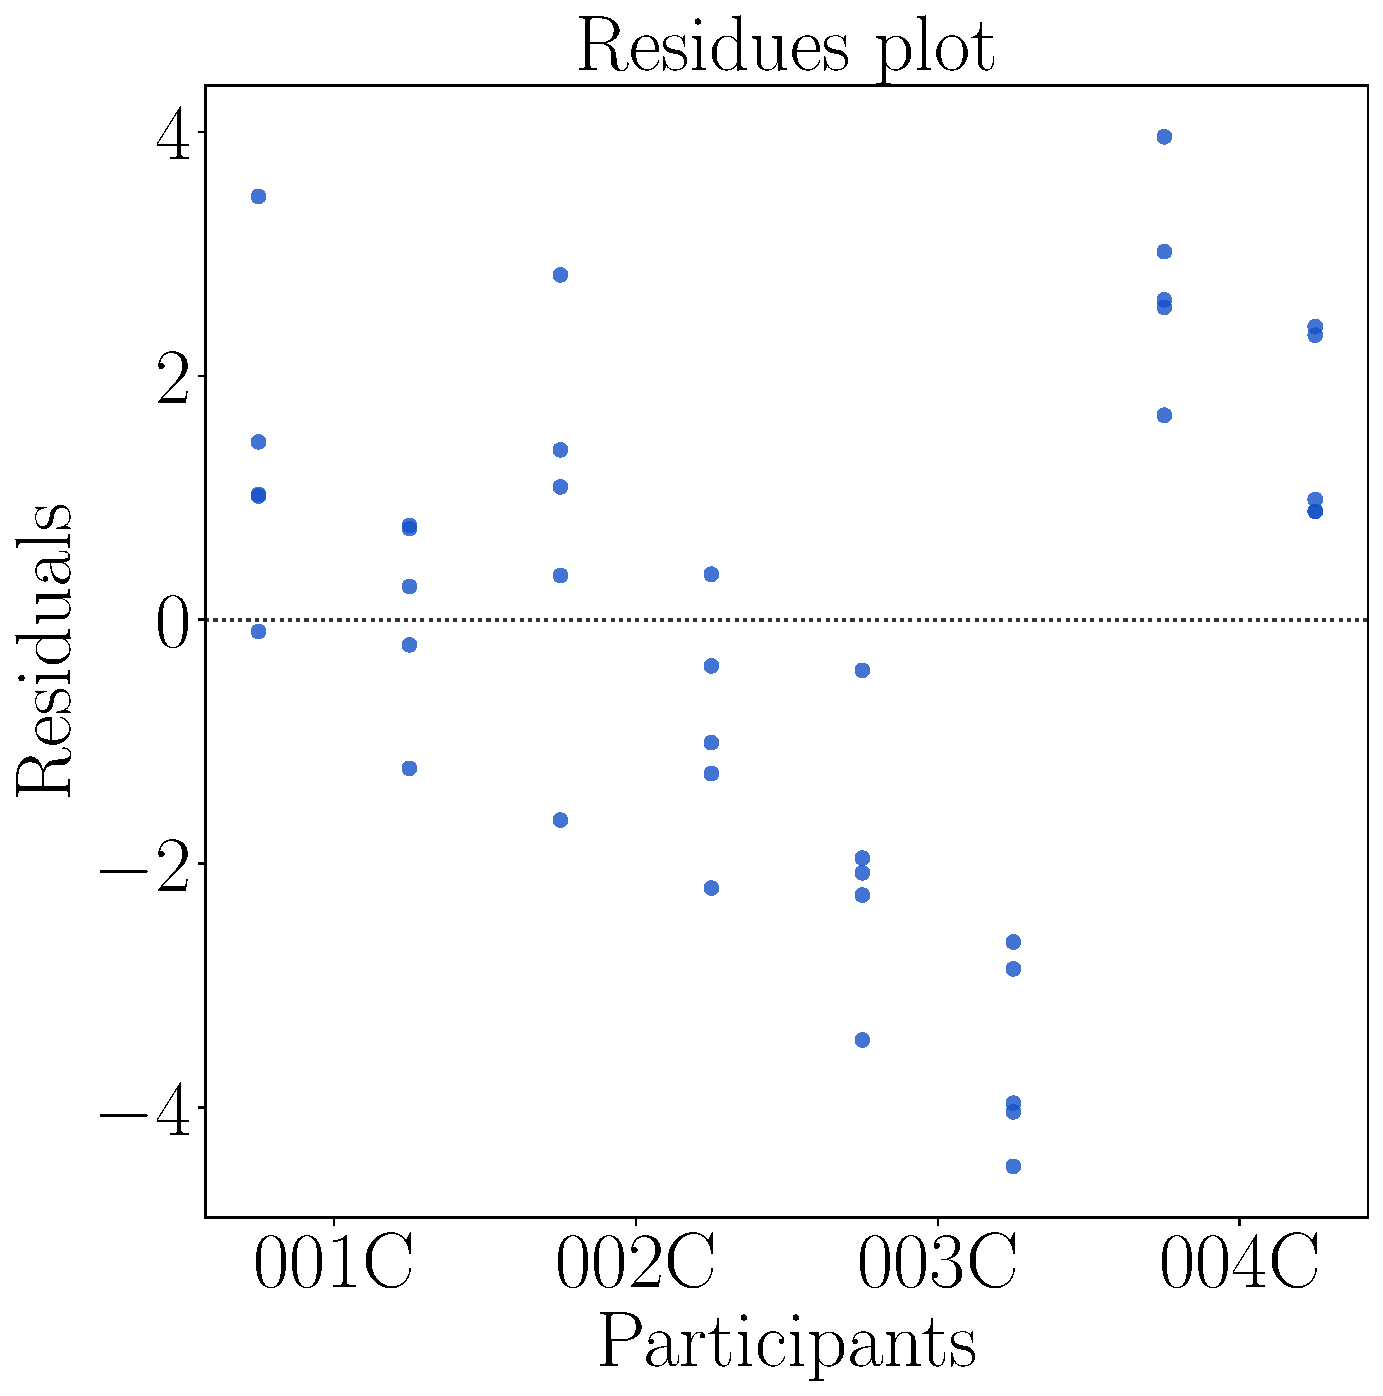
\includegraphics[width = \textwidth]{Resultados/Nasa/Figuras/pdf/residplot_nasa_avg_two_way_blind.pdf}
        \caption{Residual plot of the NASA-TLX score the blind participants on each method.}
        \label{fig:residplot_nasa_avg_two_way_blind}
    \end{minipage}
\end{figure}

Table \ref{tab:blocanova_nasa_avg_two_way_blind} brings the p-value resulting from ANOVA. In this case, both the methods and the rounds were appointed as significant variables that influence the mean value of the NASA-TLX global score. 


\begin{table}[!htb]
\centering
\caption{Anova p-value for the NASA-TLX score on each method for blinded users.}
\label{tab:blocanova_nasa_avg_two_way_blind}
\begin{tabular}{lrrrrl}
\toprule
          Source & P-Value \\
\midrule
    \    Methods & 0.029** \\
     \    Rounds & 0.022** \\
\    Interaction &   0.814 \\
\bottomrule
\end{tabular}
\end{table}



Finally, Table \ref{tab:lsd_nasa_avg_two_way_blind} presents the results of a pairwise Fisher LSD test comparing each pair of guidance methods. The results show that only "audio" is similar "base". All the other methods are different from each other.


\begin{table}[!htb]
\centering
\caption{Cross validation p-value for the NASA-TLX score on each method for blinded users.}
\label{tab:lsd_nasa_avg_two_way_blind}
\begin{tabular}{rclr}
\toprule
      \multicolumn{3}{c}{Method} &                                           Analysis \\
\midrule
              Base & $X$ & Audio &                   $H_0 : \mu_{Base} = \mu_{Audio}$ \\
        Base & $X$ & Haptic Belt &         $H_1 : \mu_{Base} \ne \mu_{Haptic Belt}**$ \\
       Base & $X$ & Virtual Cane &        $H_1 : \mu_{Base} \ne \mu_{Virtual Cane}**$ \\
            Base & $X$ & Mixture &             $H_1 : \mu_{Base} \ne \mu_{Mixture}**$ \\
       Audio & $X$ & Haptic Belt &        $H_1 : \mu_{Audio} \ne \mu_{Haptic Belt}**$ \\
      Audio & $X$ & Virtual Cane &       $H_1 : \mu_{Audio} \ne \mu_{Virtual Cane}**$ \\
           Audio & $X$ & Mixture &            $H_1 : \mu_{Audio} \ne \mu_{Mixture}**$ \\
Haptic Belt & $X$ & Virtual Cane & $H_1 : \mu_{Haptic Belt} \ne \mu_{Virtual Cane}**$ \\
     Haptic Belt & $X$ & Mixture &      $H_1 : \mu_{Haptic Belt} \ne \mu_{Mixture}**$ \\
    Virtual Cane & $X$ & Mixture &         $H_0 : \mu_{Virtual Cane} = \mu_{Mixture}$ \\
\bottomrule
\end{tabular}
\end{table}



Table \ref{tab:nasa_var_group_blind} shows the difference in the NASA-TLX global score between the first and return rounds. It shows that the "audio" difference is the lowest among all methods, while the highest difference is for the "virtual cane".


\begin{table}[!htb]
\centering
\caption{NASA-TLX score grouped by participant and visual Condition.}
\label{tab:nasa_var_group_blind}
\begin{tabular}{lrrrrrr}
\toprule
{} &   Base &  Audio & \begin{tabular}[c]{@{}l@{}}Haptic\\ Belt\end{tabular} & \begin{tabular}[c]{@{}l@{}}Virtual\\ Cane\end{tabular} & Mixture \\
Visual Condition &        &        &                                                       &                                                        &         \\
\midrule
Blind            &  -0.92 &  -0.25 &                                                 -1.21 &                                                  -1.54 &   -0.54 \\
\bottomrule
\end{tabular}
\end{table}



\FloatBarrier
\subsubsection{Adapted SAGAT}
\label{subsubsec:results_adapted_sagat_1}

In this subsection, the SAGAT questionnaire is analyzed. Its result may give an idea of the mental map the participant is drawing. For each question a participant could score 1 point or a fraction of it. The total score of each blind participant is presented on the Table \ref{tab:sagat_table_blind} and they are plotted in the Figures \ref{fig:barplot_sagat_avg_5_scene_blind}, where it is visually noticeable that the performance better the second time they visit the room. 


\begin{table}[!htb]
\centering
\caption{SAGAT global score felled by the blinded participants.}
\label{tab:sagat_table_blind}
\begin{tabular}{llrrrrr}
\toprule
     &        &   Base &  Audio & \begin{tabular}[c]{@{}l@{}}Haptic\\ Belt\end{tabular} & \begin{tabular}[c]{@{}l@{}}Virtual\\ Cane\end{tabular} & Mixture \\
Participant & Round &        &        &                                                       &                                                        &         \\
\midrule
001C & First &   6.25 &   5.50 &                                                  5.33 &                                                   5.83 &   3.500 \\
     & Return &   6.25 &   6.50 &                                                  8.50 &                                                   5.50 &   5.500 \\
002C & First &   6.75 &   4.50 &                                                  3.99 &                                                   4.50 &   6.250 \\
     & Return &   5.25 &   5.00 &                                                  4.00 &                                                   6.50 &   8.500 \\
003C & First &   7.25 &   7.50 &                                                  7.49 &                                                   4.66 &   9.000 \\
     & Return &  10.00 &  10.00 &                                                  8.50 &                                                   9.00 &   9.000 \\
004C & First &   7.50 &   6.00 &                                                  7.66 &                                                   4.99 &   6.500 \\
     & Return &   9.00 &   6.00 &                                                  9.25 &                                                   7.25 &   9.000 \\
\bottomrule
\end{tabular}
\end{table}



\begin{figure}[!htb]
    \centering
    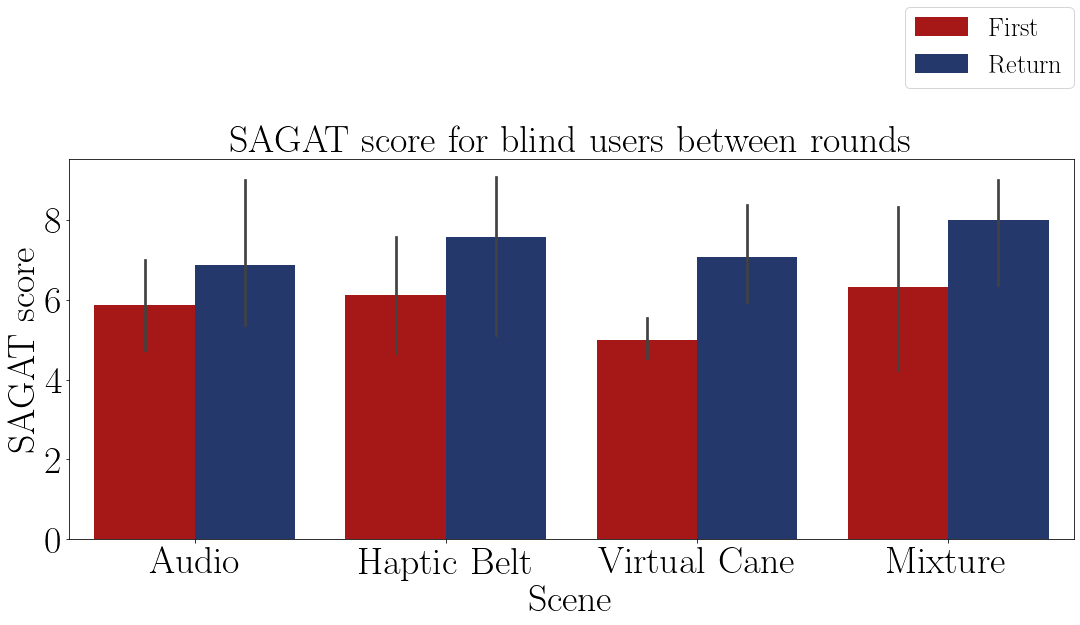
\includegraphics[width = 0.8\linewidth]{Resultados/Sagat/Figuras/png/barplot_sagat_avg_5_scene_blind.png}
    \caption{Barplot of the average SAGAT score of the blind participants on each method.}
    \label{fig:barplot_sagat_avg_5_scene_blind}
\end{figure}

The boxplot in the Figure \ref{fig:boxplot_sagat_blind_scene} shows that there are two groups of scores one with the “Base”, “Haptic Belt” and the “Mixture” methods, and the second group with the “Audio” and the “Virtual Cane” methods. The first group scored higher than the second one. The Figure \ref{fig:boxplot_sagat_blind_rounds} shows a noticible difference between the scores when grouped by their corresponding round.

\begin{figure}[!htb]
    \centering
    \begin{minipage}{0.45\textwidth}
        \centering
        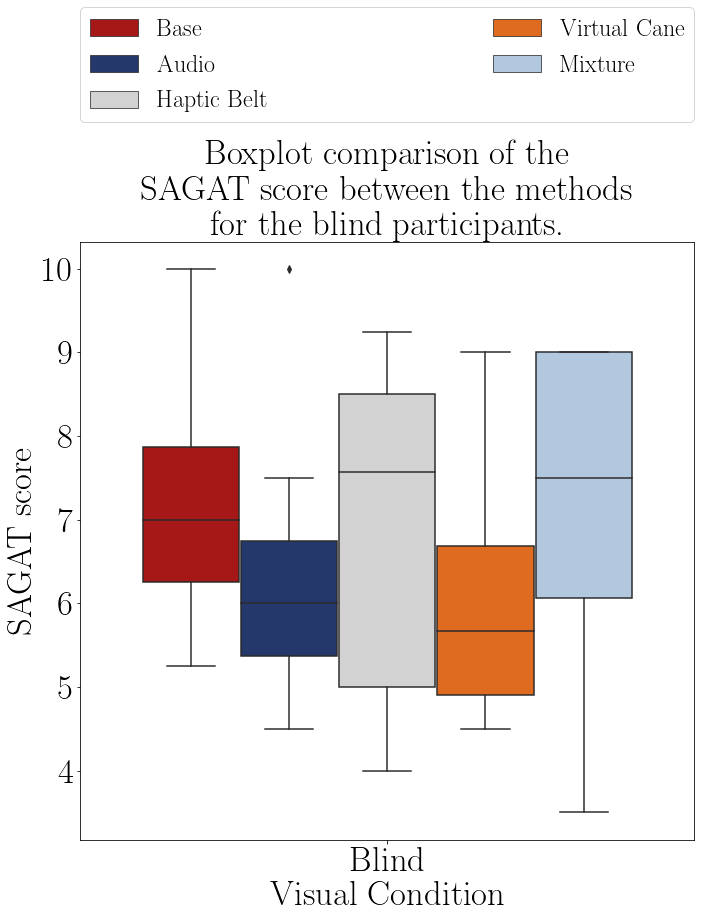
\includegraphics[width = 0.8\linewidth]{Resultados/Sagat/Figuras/png/boxplot_sagat_blind_scene.png}
        \caption{Boxplot of the SAGAT score of the blind participants grouped by method.}
        \label{fig:boxplot_sagat_blind_scene}
    \end{minipage}
    \begin{minipage}{0.45\textwidth}
        \centering
        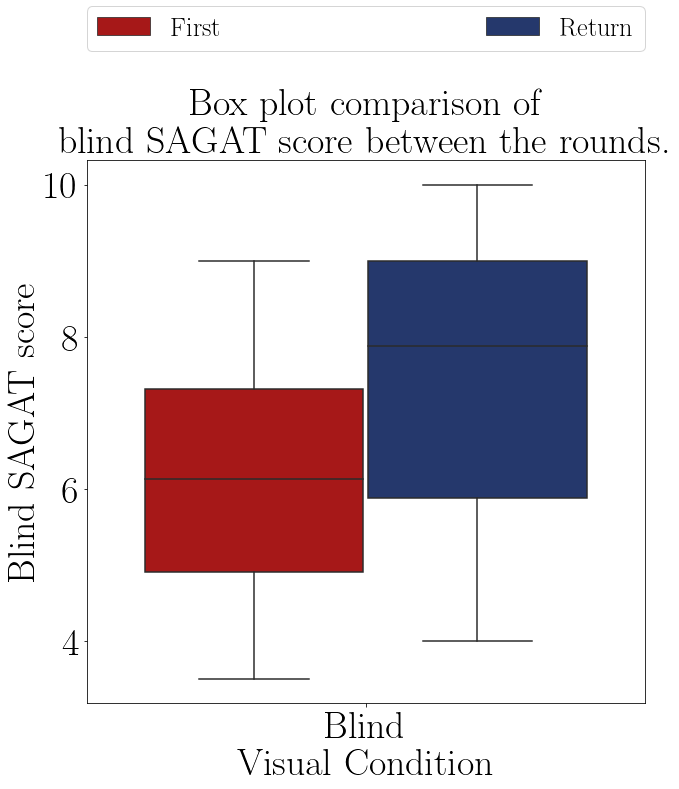
\includegraphics[width = 0.8\linewidth]{Resultados/Sagat/Figuras/png/boxplot_sagat_blind_rounds.png}
        \caption{Boxplot of the SAGAT score of the blind participants grouped by round.}
        \label{fig:boxplot_sagat_blind_rounds}
    \end{minipage}
\end{figure}

The Table \ref{tab:sagat_average_group_blind} shows the average SAGAT score in the “blind” sample and is possible to notice how the average score by the “blind” sample was lower during the “Audio” and the “Base” methods.


\begin{table}[!htb]
\centering
\caption{SAGAT score average grouped by participant and visual condition}
\label{tab:sagat_average_group_blind}
\begin{tabular}{lrrrrrr}
\toprule
{} &  Base & Audio & \begin{tabular}[c]{@{}l@{}}Haptic\\ Belt\end{tabular} & \begin{tabular}[c]{@{}l@{}}Virtual\\ Cane\end{tabular} &  Mixture \\
Visual Condition &       &       &                                                       &                                                        &          \\
\midrule
Blind            &  7.28 &  6.38 &                                                  6.84 &                                                   6.03 &    7.156 \\
\bottomrule
\end{tabular}
\end{table}




The Figures \ref{fig:qqplot_sagat_avg_two_way_blind} and \ref{fig:residplot_sagat_avg_two_way_blind} shows the distribution and variance of the Table \ref{tab:sagat_table_blind}. These Figures shows that the data are normally distributed and that the methods have a similar variance.
The Table \ref{tab:blocanova_sagat_avg_two_way_blind} shows the Anova test p-value of the SAGAT score of the "blind" sample. The round's p-values indicates that some have influence on the SAGAT score. Meaning that the participants did learn information about the room between the "First" and "Return" round. The method and the interaction between it and the round has no influence on the SAGAT score.


\begin{table}[!htb]
\centering
\caption{Anova p-value for the SAGAT score on each method for blinded users.}
\label{tab:blocanova_sagat_avg_two_way_blind}
\begin{tabular}{lrrrrr}
\toprule
               Source &  Squared sum &  DOF & Squared average &      F & \begin{tabular}[c]{@{}l@{}}P-Value \\ $(F_{0} > F)$\end{tabular} \\
\midrule
Participants (Blocks) &       48.231 &    3 &          16.077 &  9.731 &                                                                  \\
         \    Methods &        8.922 &    4 &           2.230 &  1.350 &                                                            0.277 \\
          \    Rounds &       18.975 &    1 &          18.975 & 11.485 &                                                          0.002** \\
     \    Interaction &        2.391 &    4 &           0.598 &  0.362 &                                                            0.834 \\
   Experimental Error &       44.608 &   27 &           1.652 &        &                                                                  \\
                Total &      123.127 &   39 &                 &        &                                                                  \\
\bottomrule
\end{tabular}
\end{table}



\begin{figure}[!htb]
    \centering
    \begin{minipage}{0.45\textwidth}
        \centering
        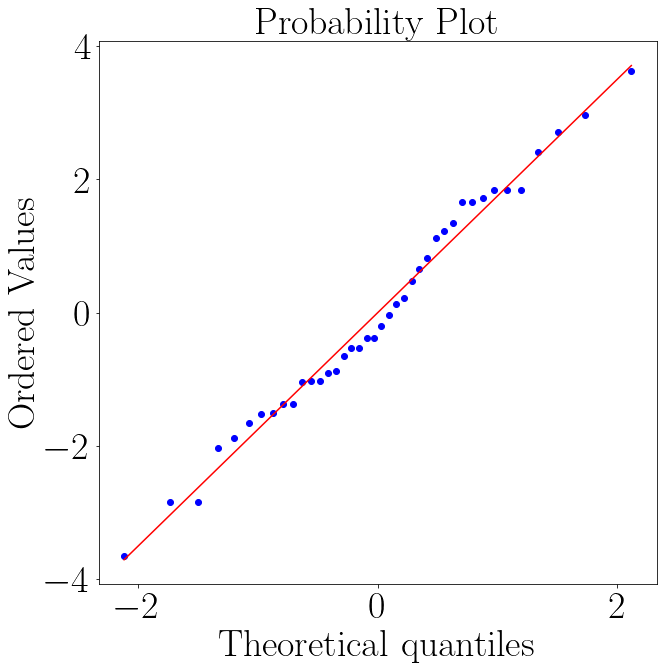
\includegraphics[width = 0.8\linewidth]{Resultados/Sagat/Figuras/png/qqplot_sagat_avg_two_way_blind.png}
        \caption{QQ plot of the SAGAT score of the blind participants on each method.}
        \label{fig:qqplot_sagat_avg_two_way_blind}
    \end{minipage}
    \begin{minipage}{0.45\textwidth}
        \centering
        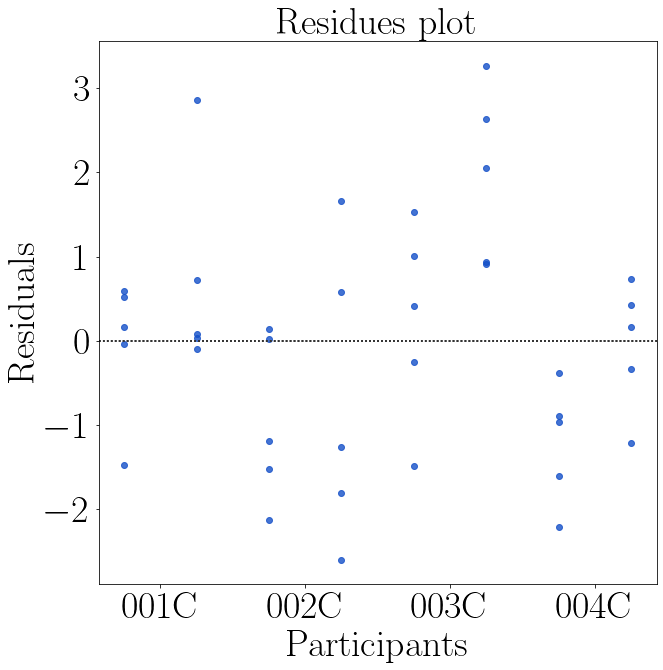
\includegraphics[width = 0.8\linewidth]{Resultados/Sagat/Figuras/png/residplot_sagat_avg_two_way_blind.png}
        \caption{Residual plot of the SAGAT score the blind participants on each method.}
        \label{fig:residplot_sagat_avg_two_way_blind}
    \end{minipage}
\end{figure}


%The Table \ref{tab:lsd_sagat_avg_two_way} presents the conclusion of a pairwise Fisher LSD test of the blind NASA-TLX score between all the guidance methods. The results show that only the "Audio" has a similar NASA-TLX score as the "Base" method, as it was also posible to notice at Figure \ref{fig:boxplot_sagat_blind_scene}.

%\input{Resultados/Sagat/Tabelas/lsd_sagat_avg_two_way}

The Table \ref{tab:sagat_var_group_blind} shows the average of the SAGAT score variation between the rounds. This table shows that the variation from the "Base" and the "Audio" was the lowest variation and the highest variation was the "Virtual Cane".


\begin{table}[!htb]
\centering
\caption{Adapted Sagat global score variation grouped by participant and visual Condition}
\label{tab:sagat_var_group_blind}
\begin{tabular}{lrrrrrr}
\toprule
{} &  Base &  Audio & \begin{tabular}[c]{@{}l@{}}Haptic\\ Belt\end{tabular} & \begin{tabular}[c]{@{}l@{}}Virtual\\ Cane\end{tabular} & Mixture \\
Visual Condition &       &        &                                                       &                                                        &         \\
\midrule
Blind            &  8.93 &  15.66 &                                                 23.49 &                                                  44.30 &   32.90 \\
\bottomrule
\end{tabular}
\end{table}



The Figures \ref{fig:qqplot_sagat_var_blind} and \ref{fig:residplot_sagat_var_blind} shows the distribution and variance of the SAGAT score variation of the Table \ref{tab:sagat_table_blind}. These Figures shows that the data are normally distributed and that the methods have a similar variance.
The Table \ref{tab:blocanova_sagat_var_blind} shows the Anova test p-value of the SAGAT score of the "blind" sample between the guidance methods. The p-value indicates that there are no difference between the variation in any method. 


\begin{table}[!htb]
\centering
\caption{Anova p-value for the SAGAT score variation on each method for blinded users.}
\label{tab:blocanova_sagat_var_blind}
\begin{tabular}{lrrrrr}
\toprule
               Source &  Squared sum &  DOF & Squared average &     F & \begin{tabular}[c]{@{}l@{}}P-Value \\ $(F_{0} > F)$\end{tabular} \\
\midrule
Participants (blocks) &     1176.902 &    3 &         782.885 & 0.473 &                                                                  \\
               Method &     3131.542 &    4 &         392.301 & 0.944 &                                                            0.472 \\
   Experimental error &     9956.458 &   12 &         829.705 &       &                                                                  \\
                Total &    14264.902 &   19 &                 &       &                                                                  \\
\bottomrule
\end{tabular}
\end{table}



\begin{figure}[!htb]
    \centering
    \begin{minipage}{0.45\textwidth}
        \centering
        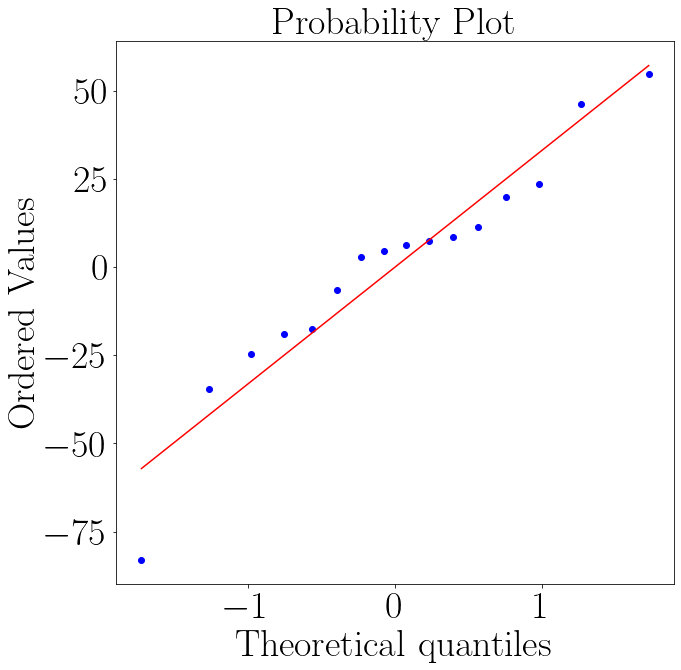
\includegraphics[width = 0.8\linewidth]{Resultados/Sagat/Figuras/png/qqplot_sagat_var_sight.png}
        \caption{QQ plot of the SAGAT score variation of the blind participants on each method.}
        \label{fig:qqplot_sagat_var_blind}
    \end{minipage}
    \begin{minipage}{0.45\textwidth}
        \centering
        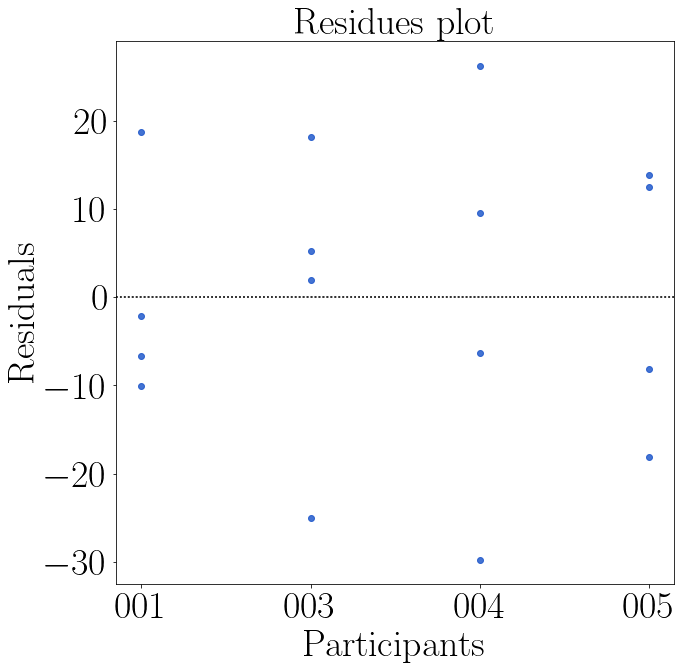
\includegraphics[width = 0.8\linewidth]{Resultados/Sagat/Figuras/png/residplot_sagat_var_sight.png}
        \caption{Residual plot of the SAGAT score variation of the blind participants on each method.}
        \label{fig:residplot_sagat_var_blind}
    \end{minipage}
\end{figure}

%The Table \ref{tab:lsdbloc_nasa_var} presents the conclusion of a pairwise Fisher LSD test of the blind NASA-TLX score between all the guidance methods. The results show that all methods have similar variations.

%
\begin{table}[!htb]
\centering
\caption{Cross validation p-value for the NASA-TLX score variation on each method for blinded users.}
\label{tab:lsdbloc_nasa_var}
\begin{tabular}{rclr}
\toprule
      \multicolumn{3}{c}{Method} &                                       Analysis \\
\midrule
              Base & $X$ & Audio &           $H_1 : \mu_{Base} \ne \mu_{Audio}**$ \\
        Base & $X$ & Haptic Belt &         $H_0 : \mu_{Base} = \mu_{Haptic Belt}$ \\
       Base & $X$ & Virtual Cane &    $H_1 : \mu_{Base} \ne \mu_{Virtual Cane}**$ \\
            Base & $X$ & Mixture &             $H_0 : \mu_{Base} = \mu_{Mixture}$ \\
       Audio & $X$ & Haptic Belt &    $H_1 : \mu_{Audio} \ne \mu_{Haptic Belt}**$ \\
      Audio & $X$ & Virtual Cane &   $H_1 : \mu_{Audio} \ne \mu_{Virtual Cane}**$ \\
           Audio & $X$ & Mixture &            $H_0 : \mu_{Audio} = \mu_{Mixture}$ \\
Haptic Belt & $X$ & Virtual Cane & $H_0 : \mu_{Haptic Belt} = \mu_{Virtual Cane}$ \\
     Haptic Belt & $X$ & Mixture &  $H_1 : \mu_{Haptic Belt} \ne \mu_{Mixture}**$ \\
    Virtual Cane & $X$ & Mixture & $H_1 : \mu_{Virtual Cane} \ne \mu_{Mixture}**$ \\
\bottomrule
\end{tabular}
\end{table}



To close up, according to the ANOVA test at Table \ref{tab:blocanova_sagat_avg_two_way_blind} the methods caused no reaction on the SAGAT score, but the rounds did. That means that the participants were able in all methods to learn a little about their environment and that learning impacted their environmental perception in the next round. The fact that the test has not found any influence of the methods on the SAGAT score may be because of the small sample size, since it is posible to notice a difference between the methods at Figure \ref{fig:boxplot_sagat_blind_scene}. Also the interaction between method and round caused no influence in the Sagat score. According to the ANOVA test at Table \ref{tab:blocanova_sagat_var_blind}, the methods did not influenced the SAGAT score.

\FloatBarrier
\subsubsection{Guidance method's questionnaire.}
\label{subsubsec:results_questionnaires}

Finally, the data from the questionnaire for evaluating the user experience with each guidance method is also analysed. The higher the score, the more satisfied the user is with the method. It is important to observe that this analysis does not include the ‘base’ method as the questions are specific about each method and the ‘base’ may vary among the participants. Also, there is no distinction between first and return rounds. Each questionnaire is answered only once for each method

Table \ref{tab:questionnaire_average_blind} presents the score attributed to each method by each participant. The mean values are plotted in the Figure \ref{fig:barplot_questionnaire_scene_blind} and show a dissatisfaction with the methods that only use vibration for communicating with the participant, i.e., the haptic belt and the virtual cane. 


\begin{table}[!htb]
\centering
\caption{ Guidance method questionnaire score felled by the blinded participants.}
\label{tab:questionnaire_average_blind}
\begin{tabular}{llrrrrr}
\toprule
{} &  Audio &  \begin{tabular}[c]{@{}l@{}}Haptic\\ Belt\end{tabular} &  \begin{tabular}[c]{@{}l@{}}Virtual\\ Cane\end{tabular} &  Mixture \\
Participant &        &                                                        &                                                         &          \\
\midrule
001C        &  0.774 &                                                  0.543 &                                                   0.629 &    0.865 \\
002C        &  0.857 &                                                  0.743 &                                                   0.543 &    0.935 \\
003C        &  0.929 &                                                  0.571 &                                                   0.543 &    0.745 \\
004C        &  0.881 &                                                  0.486 &                                                   0.400 &    0.730 \\
\bottomrule
\end{tabular}
\end{table}



\begin{figure}[!htb]
    \centering
    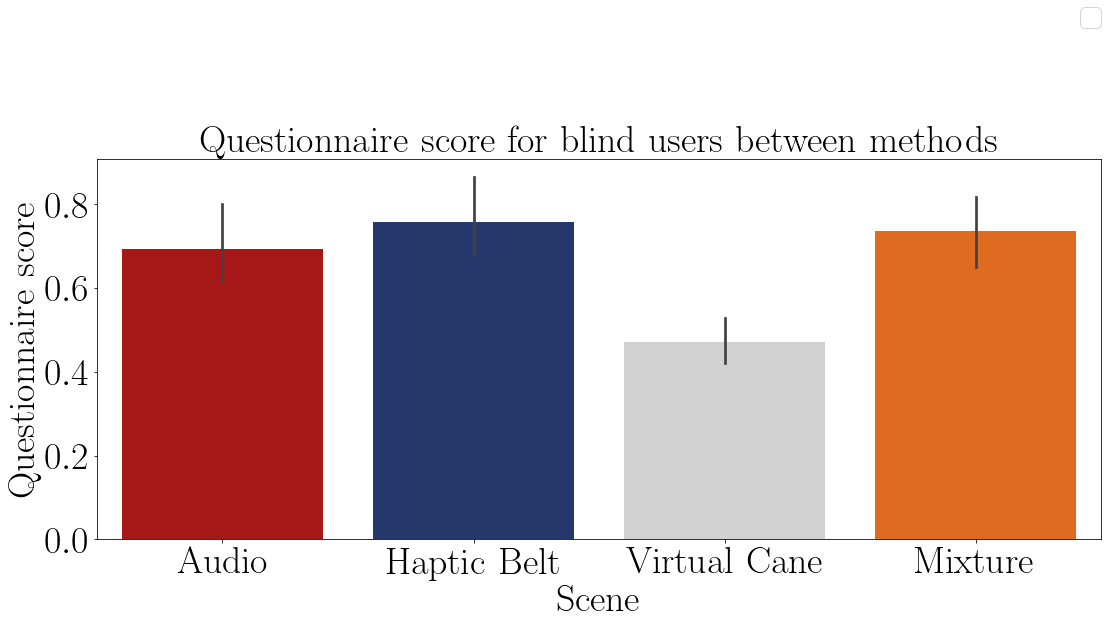
\includegraphics[width = 0.8\linewidth]{Resultados/Questionario/Figuras/png/barplot_questionnaire_scene_blind.png}
    \caption{Barplot of the average questionaire score of the blind participants on each method.}
    \label{fig:barplot_questionnaire_scene_blind}
\end{figure}

Figure \ref{fig:boxplot_quest_blind_scene} brings the questionnaire boxplot, which clearly shows the difference between two groups: haptic belt and virtual cane, and audio and mixture. 

\begin{figure}[!htb]
    \centering
    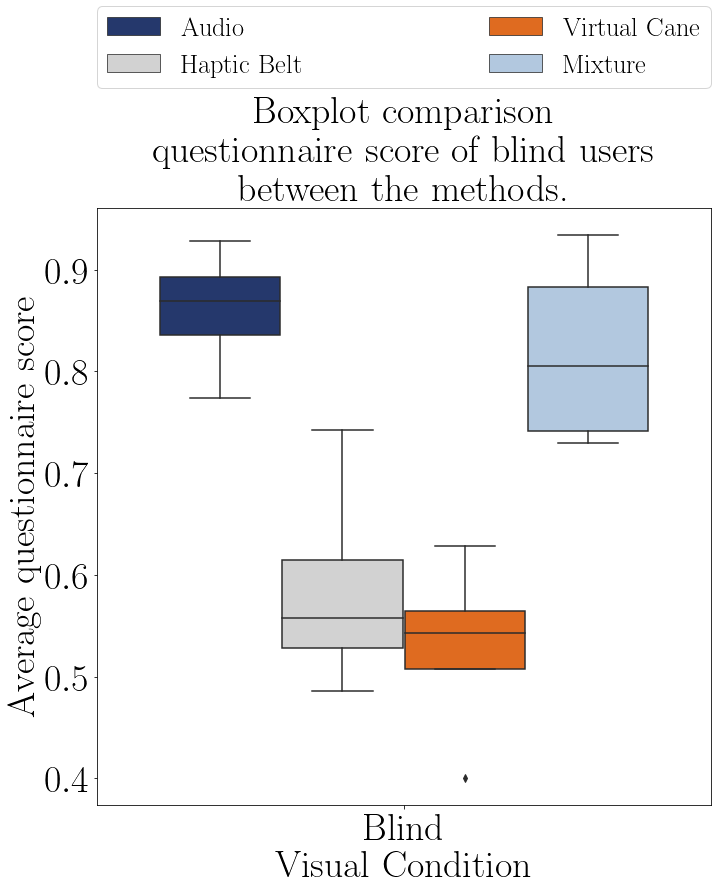
\includegraphics[width = 0.6\linewidth]{Resultados/Questionario/Figuras/png/boxplot_questionnaire_scene_blind.png}
    \caption{Boxplot of the questionaire score of the blind participants grouped by method.}
    \label{fig:boxplot_quest_blind_scene}
\end{figure}

%The Table \ref{tab:questionnaire_average_group_blind} show the the average questionnaire score on each method. It also shows a disatisfaction with the haptic devices alone.
%
%
\begin{table}[!htb]
\centering
\caption{Guidance method questionnaire average score for the blind participants.}
\label{tab:questionnaire_average_group_blind}
\begin{tabular}{lrrrrr}
\toprule
{} & Audio & Haptic Belt & Virtual Cane & Mixture \\
Visual Condition &       &             &              &         \\
\midrule
Blind            &  0.86 &        0.59 &         0.53 &    0.82 \\
\bottomrule
\end{tabular}
\end{table}



Following, Figures \ref{fig:qqplot_questionnaires} and \ref{fig:residplot_questionnaires} shows that the data follows a normal distribution. However, the residual variance is not exactly homogenous among the participants. 

\begin{figure}[!htb]
    \centering
    \begin{minipage}{0.45\textwidth}
        \centering
        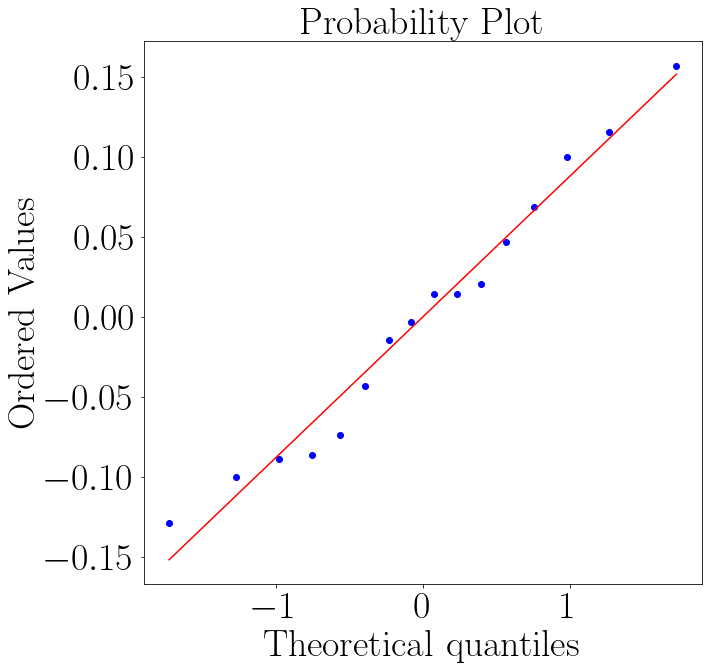
\includegraphics[width = 0.8\linewidth]{Resultados/Questionario/Figuras/png/qqplot_questionnaires.png}
        \caption{QQ plot of the questionnaire score of the blind participants on each method.}
        \label{fig:qqplot_questionnaires}
    \end{minipage}
    \begin{minipage}{0.45\textwidth}
        \centering
        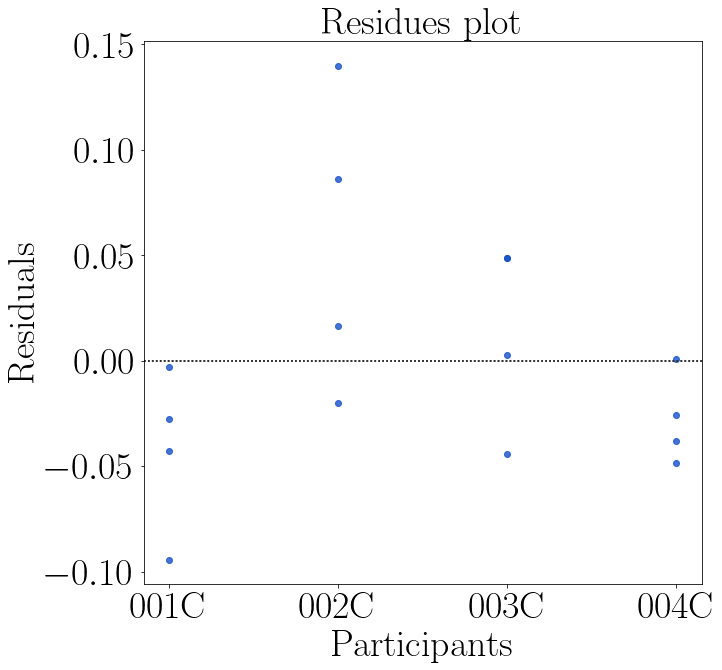
\includegraphics[width = 0.8\linewidth]{Resultados/Questionario/Figuras/png/residplot_questionnaires.png}
        \caption{Residual plot of the questionnaire score the blind participants on each method.}
        \label{fig:residplot_questionnaires}
    \end{minipage}
\end{figure}

The results of ANOVA are presented in Table  \ref{tab:blocanova_questionnaire} and shows that the method, with a p-value of 0.001, is indeed a significant variable that affects the user satisfaction.


\begin{table}[!htb]
\centering
\caption{Anova p-value for the questionnaire score on each method for blinded users.}
\label{tab:blocanova_questionnaire}
\begin{tabular}{lrrrrr}
\toprule
               Source &  Squared sum &  DOF & Squared average &      F & \begin{tabular}[c]{@{}l@{}}P-Value \\ $(F_{0} > F)$\end{tabular} \\
\midrule
Participants (blocks) &        0.042 &    3 &           0.110 &  2.014 &                                                                  \\
               Method &        0.329 &    3 &           0.014 & 15.677 &                                                          0.001** \\
   Experimental error &        0.063 &    9 &           0.007 &        &                                                                  \\
                Total &        0.434 &   15 &                 &        &                                                                  \\
\bottomrule
\end{tabular}
\end{table}



In order to complement the ANOVA analysis, the pairwise comparison of the methods, obtained from the Fisher LSD test, is presented in Table \ref{tab:lsd_questionnaire}. The results show that ‘audio’ and ‘mixture’ are equivalent from the perspective of user satisfaction. All the other comparisons indicate there is a difference between the methods.


\begin{table}[!htb]
\centering
\caption{Cross validation p-value for the questionnaire score on each method for blinded users.}
\label{tab:lsd_questionnaire}
\begin{tabular}{rclr}
\toprule
      \multicolumn{3}{c}{Method} &                                           Analysis \\
\midrule
       Audio & $X$ & Haptic Belt &        $H_1 : \mu_{Audio} \ne \mu_{Haptic Belt}**$ \\
      Audio & $X$ & Virtual Cane &       $H_1 : \mu_{Audio} \ne \mu_{Virtual Cane}**$ \\
           Audio & $X$ & Mixture &                $H_0 : \mu_{Audio} = \mu_{Mixture}$ \\
Haptic Belt & $X$ & Virtual Cane & $H_1 : \mu_{Haptic Belt} \ne \mu_{Virtual Cane}**$ \\
     Haptic Belt & $X$ & Mixture &          $H_0 : \mu_{Haptic Belt} = \mu_{Mixture}$ \\
    Virtual Cane & $X$ & Mixture &     $H_1 : \mu_{Virtual Cane} \ne \mu_{Mixture}**$ \\
\bottomrule
\end{tabular}
\end{table}



Additional to the scores, the participants also expressed their dissatisfaction in the answers to the open questions of the questionnaire, where they commented that the haptic belt and the virtual cane are confusing, are not enough precise, and are very different from what they are used to.

\FloatBarrier

\subsection{Physiological data}

During the experiment, data from two physiological sensors were captured: ECG and GSR. As commonly found in the literature, these data are used to assess mental workload. The corresponding analysis is presented in this section.

\subsubsection{Electrocardiogram (ECG) data}
\label{subsubsec:results_ecg_1}

As previously stated, the ECG analysis is based on two variables: the heartrate (BPM – beats per minute) and heartrate variance (SDNN – standard deviation of NN intervals). 

After the experiment, the ECG signal processing is organized in the following steps (Figure \ref{fig:ecg_algorithim}): 

\begin{itemize}
    \item Filtering and removing outliers. Since the participants moved during the whole experience, the sensors also captured some noise data.
    \item Normalization between -1 and 1;
    \item Peak detection and evaluation – if the results were not of good quality, the peak detection method's parameters were adjusted to improve it; 
    \item Calculation of BPM using Kubius HRV Standard;
    \item Calculation of SDNN using Kubius HRV Standard.
\end{itemize}

\begin{figure}[H]
    \centering
    \tikzstyle{start} = [rectangle, rounded corners, minimum width=4cm, minimum height=1.0cm,text centered, draw=black, fill=white!30, text width=3cm]
\tikzstyle{process} = [rectangle, minimum width=4cm, minimum height=1.0cm, text centered, draw=black, fill=white!30, text width=3.5cm]
\tikzstyle{decision} = [diamond, minimum width=3.5cm, minimum height=1.0cm,  text centered, text width=3.5cm, draw=black, fill=white!30]
\tikzstyle{arrow_flow} = [ccmDBlue, rounded corners, line width = 2mm, ->]
\tikzstyle{arrow_return} = [ccmRed, rounded corners, line width = 2mm, ->]

\begin{tikzpicture}[node distance=2cm]
    \centering
    \node (start) [start] {Collect the ECG Data};
    \node (read) [process, below of=start,yshift=-0.5cm] {Python - Read the ECG file};
    \node (outlier) [process, aspect=2.5, below of=read, yshift=-0.5cm, text width=4cm] {Python - Remove the outlier noise};
    \node (normalize) [process, aspect=2.5, below of=outlier, yshift=-0.5cm] {Python - Normalize (-1 and 1)};
    \node (findPeaks) [process, aspect=2.5, below of=normalize, yshift=-0.5cm] {Python - Run peak finder};
    \node (graphical) [decision, aspect=2.5, below of=findPeaks, yshift=-1cm] {Graphical analysis};

    \node (no_graphical) [process, below of=graphical, yshift=-0.75cm] {Python - Tune the peak finder};

    \node (yes_graphical) [process, right of=graphical, xshift=2.5cm, yshift=2.5cm]{Python - Calculate the time difference between peaks};
    \node (savePeak) [process, above of=yes_graphical, yshift=1.0cm, text width=4cm]{Python - Save the peak file};
    \node (readPeak) [process, above of=savePeak, yshift=0.5cm, text width=4cm] {Kubius - Read the peak file};
    \node (analysis) [process, above of=readPeak, yshift=0.5cm, text width=4cm] {Kubius - Run Analysis};
    \node (saveAnalysis) [process, right of=analysis, xshift=2.5cm, yshift=-2.5cm] {Kubius - Save a report file};
    \node (readAnalysis) [process, below of=saveAnalysis, yshift=-1.0cm] {Python - Read report file};
    
    \draw [arrow_flow] (start.south) -- (read.north);
    \draw [arrow_flow] (read.south) -- (outlier.north);
    \draw [arrow_flow] (outlier.south) -- (normalize.north);
    \draw [arrow_flow] (normalize.south) -- (findPeaks.north);
    \draw [arrow_flow] (findPeaks.south) -- (graphical.north);
    
    \draw [arrow_flow] (graphical.east) -- node[anchor=north] {Peaks fit} +(1.8,0) -- (yes_graphical.south);
    \draw [arrow_flow] (yes_graphical.north) -- (savePeak.south);
    \draw [arrow_flow] (savePeak.north) -- (readPeak.south);
    \draw [arrow_flow] (readPeak.north) -- (analysis.south);
    \draw [arrow_flow] (analysis.east) -- ++(2.4,0) -- (saveAnalysis.north);
    \draw [arrow_flow] (saveAnalysis.south) -- (readAnalysis.north);
    \draw [arrow_return] (readAnalysis) -- ++(0,-1.5) -- ++(2.25,0) -- (11.25,1) -- (-3,1) -- (-3,-2.5) -- (read.west);
    
    \draw [arrow_flow] (graphical.west) -- ++(-0.3,0) -- node[anchor=south west] {Peaks} node[anchor=west] {fit not} ++(0,-2.75) -- (no_graphical.west);

    \draw [arrow_return] (no_graphical.north) -- (graphical.south);
    
\end{tikzpicture}
    \caption{ECG's data treatment algorithim.}
    \label{fig:ecg_algorithim}
\end{figure}

At the beginning of each experiment, a baseline was collected to establish a comparison between the relaxed state of the participant and the scenes' induced state. However, the results were not consistent.  During the experiment, it was expected that the heartrate would increase compared to the baseline because the participants were at rest. However, for most of the participants, it decreased, indicating a systematic problem may have occurred. Due to this fact, the analysis is based only on absolute values.

\paragraph{Analysis of the heartbeat frequency (BPM)}\mbox{}\\

Table \ref{tab:bpm_table_blind} presents the heart rate of each blind participant for each guidance method. If the variation between the First and the Return round is positive, it means that the user had an increase on his/her mental workload and vice-versa. It is possible to observe that there is no systematic difference between the methods. Also, there are significant differences among the participants, with some presenting values significantly lower than others.


\begin{table}[!htb]
\centering
\caption{Average BPM felled by the blinded participants [BPM].}
\label{tab:bpm_table_blind}
\begin{tabular}{llrrrrr}
\toprule
     &        &   Base &  Audio & \begin{tabular}[c]{@{}l@{}}Haptic\\ Belt\end{tabular} & \begin{tabular}[c]{@{}l@{}}Virtual\\ Cane\end{tabular} & Mixture \\
Participant & Round &        &        &                                                       &                                                        &         \\
\midrule
001C & First &  75.75 &  60.71 &                                                 71.17 &                                                  59.07 &   68.24 \\
     & Return &  71.05 &  58.61 &                                                 66.22 &                                                  64.20 &   70.76 \\
002C & First &  48.69 &  38.67 &                                                 48.74 &                                                  46.89 &   52.23 \\
     & Return &  52.46 &  47.58 &                                                 58.97 &                                                  56.75 &   58.25 \\
003C & First &  68.37 &  69.89 &                                                 70.95 &                                                  69.41 &   66.94 \\
     & Return &  67.34 &  67.44 &                                                 69.68 &                                                  68.82 &   67.37 \\
004C & First &  75.09 &  73.55 &                                                 73.70 &                                                  71.94 &   74.03 \\
     & Return &  74.74 &  74.79 &                                                 74.02 &                                                  72.69 &   67.34 \\
\bottomrule
\end{tabular}
\end{table}



Figure \ref{fig:barplot_ecg_bpm_5_scene_blind} presents the mean heart rate. It shows a slight increase in the heartrate between the rounds, except for the base method, indicating that the participants had a higher Mental Workload on the return round.

\begin{figure}[!htb]
    \centering
    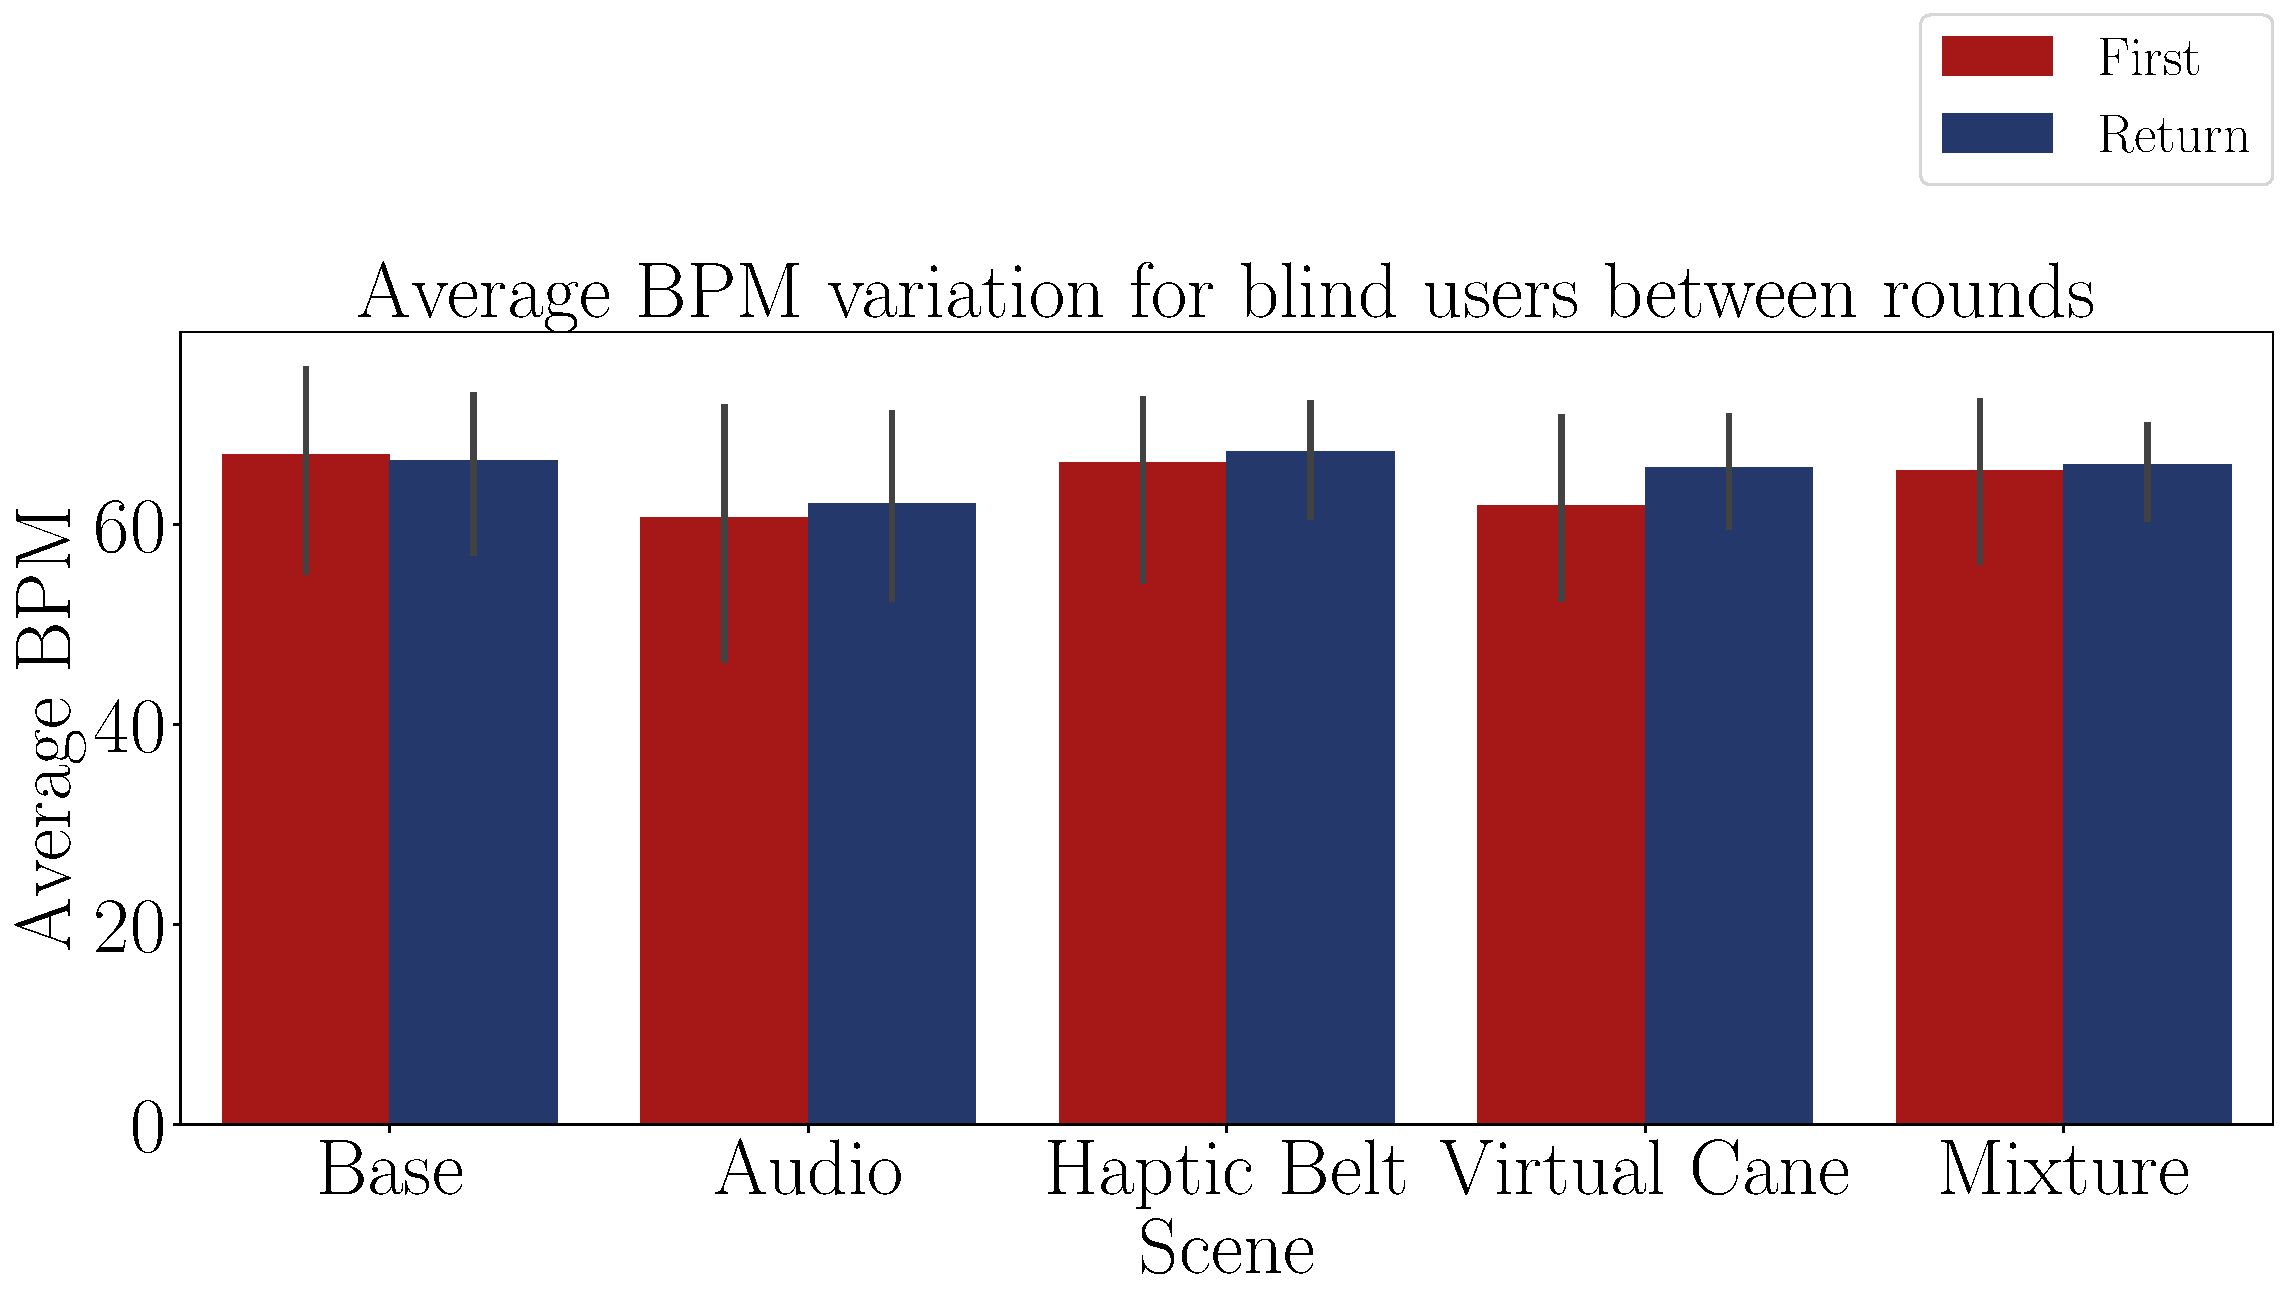
\includegraphics[width = \textwidth]{Resultados/ECG/Figuras/pdf/barplot_ecg_bpm_5_scene_blind.pdf}
    \caption{Barplot of the average BPM of the blind participants on each method.}
    \label{fig:barplot_ecg_bpm_5_scene_blind}
\end{figure}

%The Table \ref{tab:bpm_average_group_blind} show the average heartbeat frequency variation between the rounds of each group. As it was shown in the Figure \ref{fig:barplot_ecg_bpm_5_scene_blind}, only the Base method has a negative average variaton between the rounds. It is also posible to see that the Virtual Cane variation was the highest, hence it was also the highest mental workload.
% 
%
\begin{table}[!htb]
\centering
\caption{ECG average BPM  for each method of the blind participants.}
\label{tab:bpm_average_group_blind}
\begin{tabular}{lrrrrr}
\toprule
{} &   Base & Audio & Haptic Belt & Virtual Cane & Mixture \\
Visual Condition &        &       &             &              &         \\
\midrule
Blind            &  -0.58 &  1.40 &        1.09 &         3.79 &    0.57 \\
\bottomrule
\end{tabular}
\end{table}



Figures \ref{fig:boxplot_ecg_bpm_blind_scene} and \ref{fig:boxplot_ecg_bpm_blind_rounds} brings the corresponding boxplot, grouped by method and round. In both cases, it is not possible to observe significant differences among the methods or rounds.

\begin{figure}[!htb]
    \centering
    \begin{minipage}{0.45\textwidth}
        \centering
        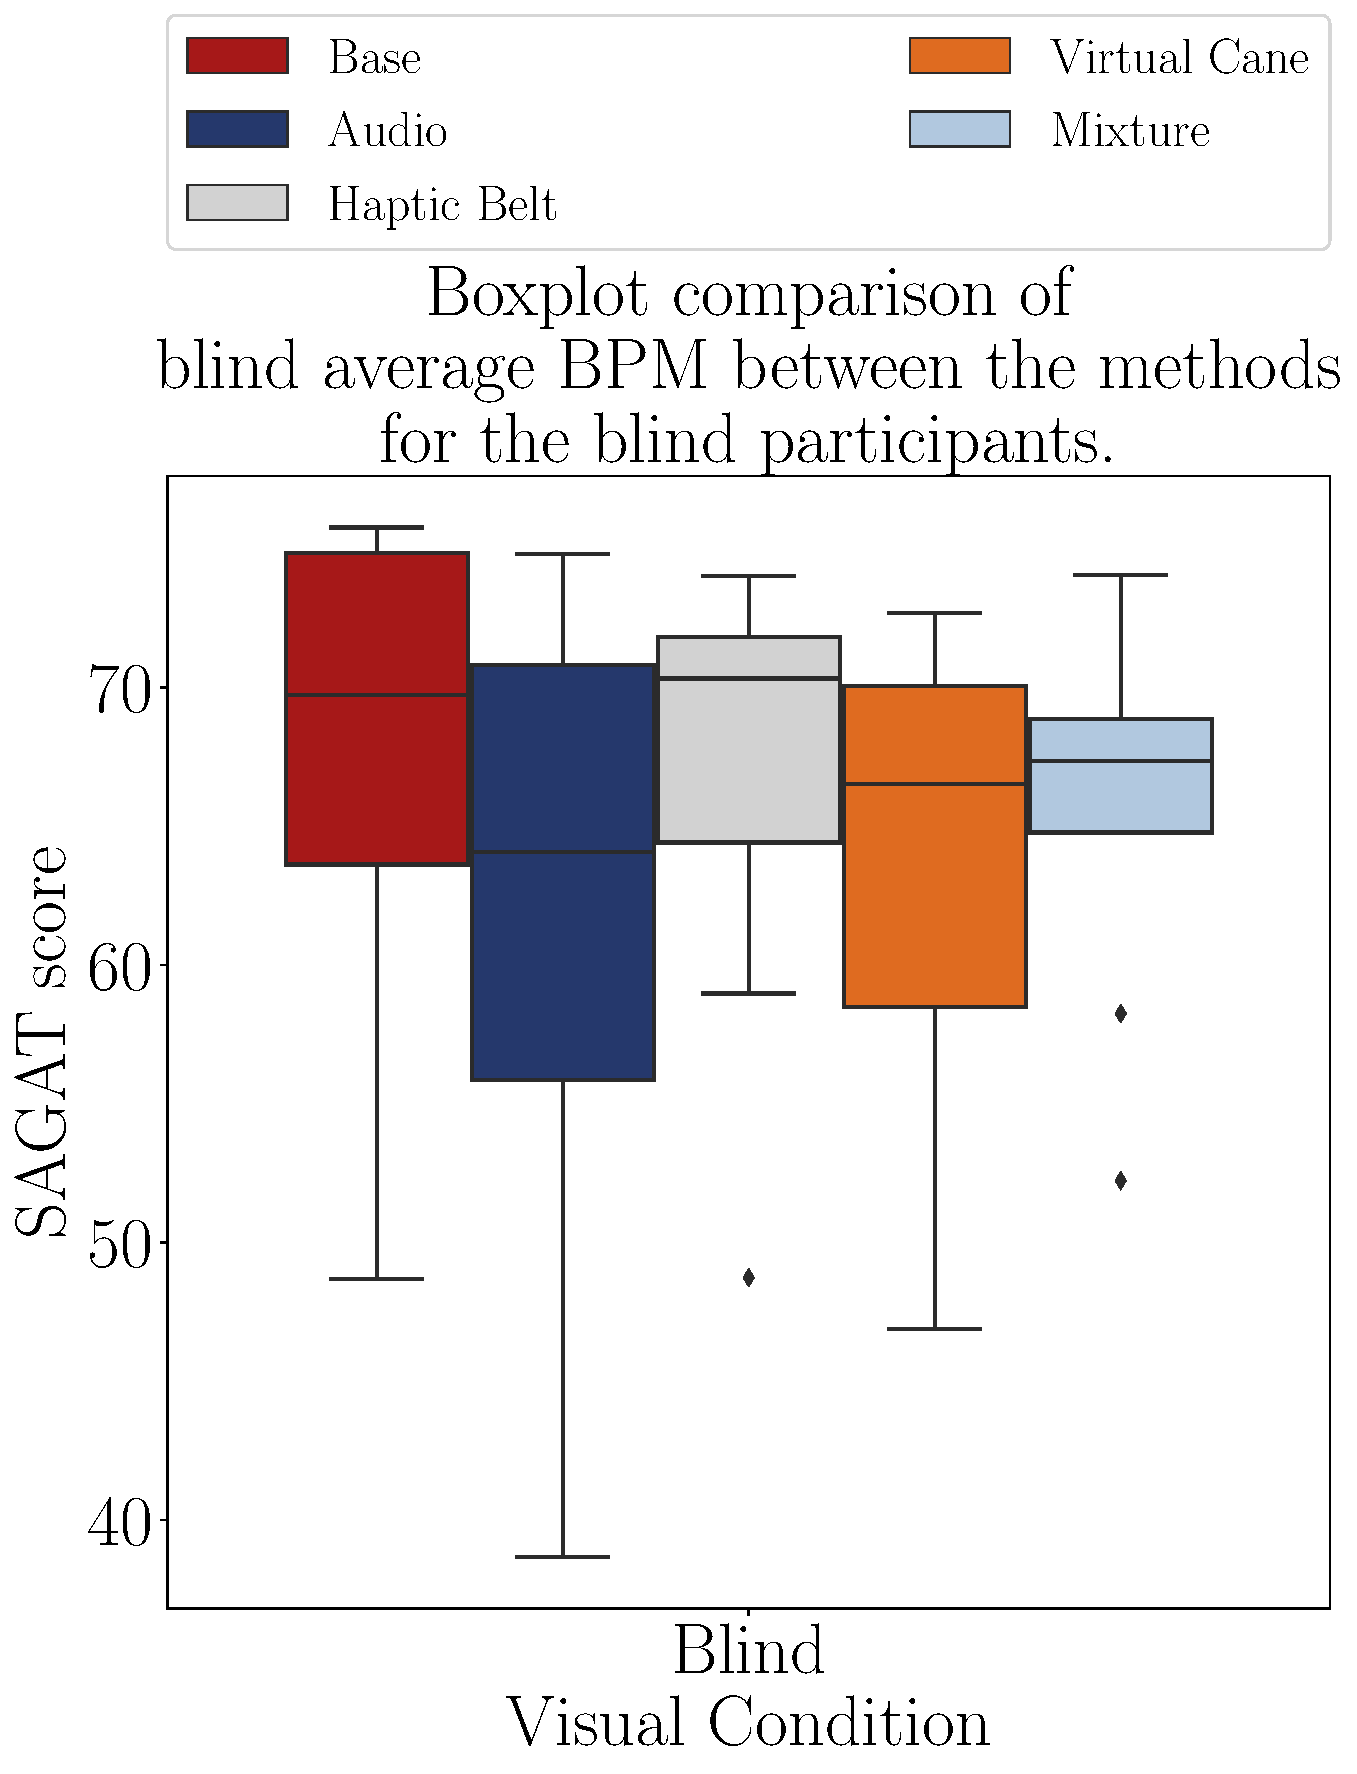
\includegraphics[width = \textwidth]{Resultados/ECG/Figuras/pdf/boxplot_ecg_bpm_blind_scene.pdf}
        \caption{Boxplot of the BPM of the blind participants grouped by the methods.}
        \label{fig:boxplot_ecg_bpm_blind_scene}
    \end{minipage}
    \begin{minipage}{0.075\textwidth}
        \hfill
    \end{minipage}
    \begin{minipage}{0.45\textwidth}
        \centering
        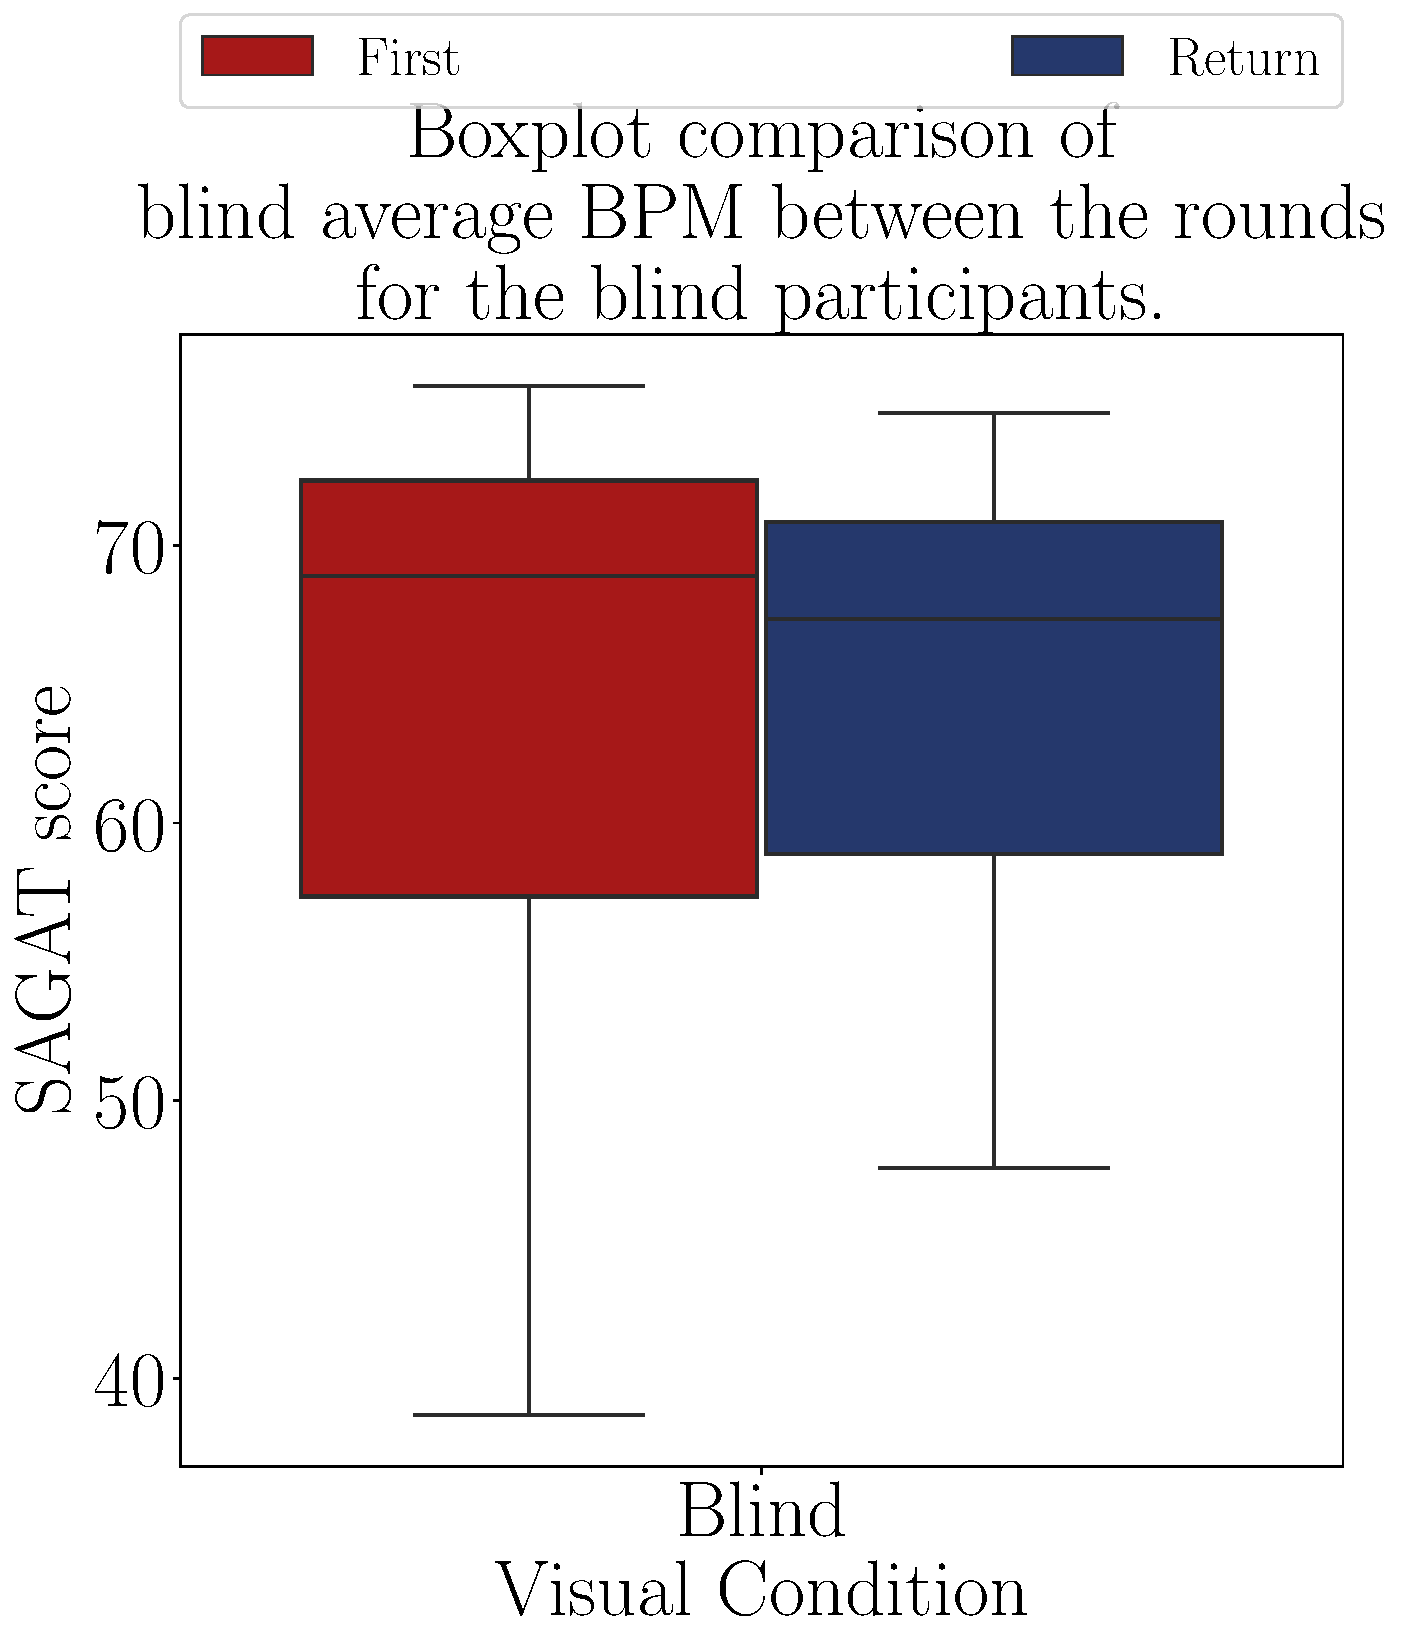
\includegraphics[width = \textwidth]{Resultados/ECG/Figuras/pdf/boxplot_ecg_bpm_blind_rounds.pdf}
        \caption{Boxplot of the BPM of the blind participants grouped by the rounds.}
        \label{fig:boxplot_ecg_bpm_blind_rounds}
    \end{minipage}
\end{figure}

Figures \ref{fig:qqplot_bpm_two_way_blind} and \ref{fig:residplot_bpm_two_way_blind} bring the QQ Plot and residual distribution. The last one shows that the participants do not have a similar variance, which may jeopardize the results of ANOVA. Considering this limitation, Table \ref{tab:bpm_table_blind} brings the p-value obtained by ANOVA, which confirmed the previous analysis, as it does not indicate a significant influence of either the guidance methods or the rounds in the participants' heartrate. 

\begin{figure}[!htb]
    \centering
    \begin{minipage}{0.45\textwidth}
        \centering
        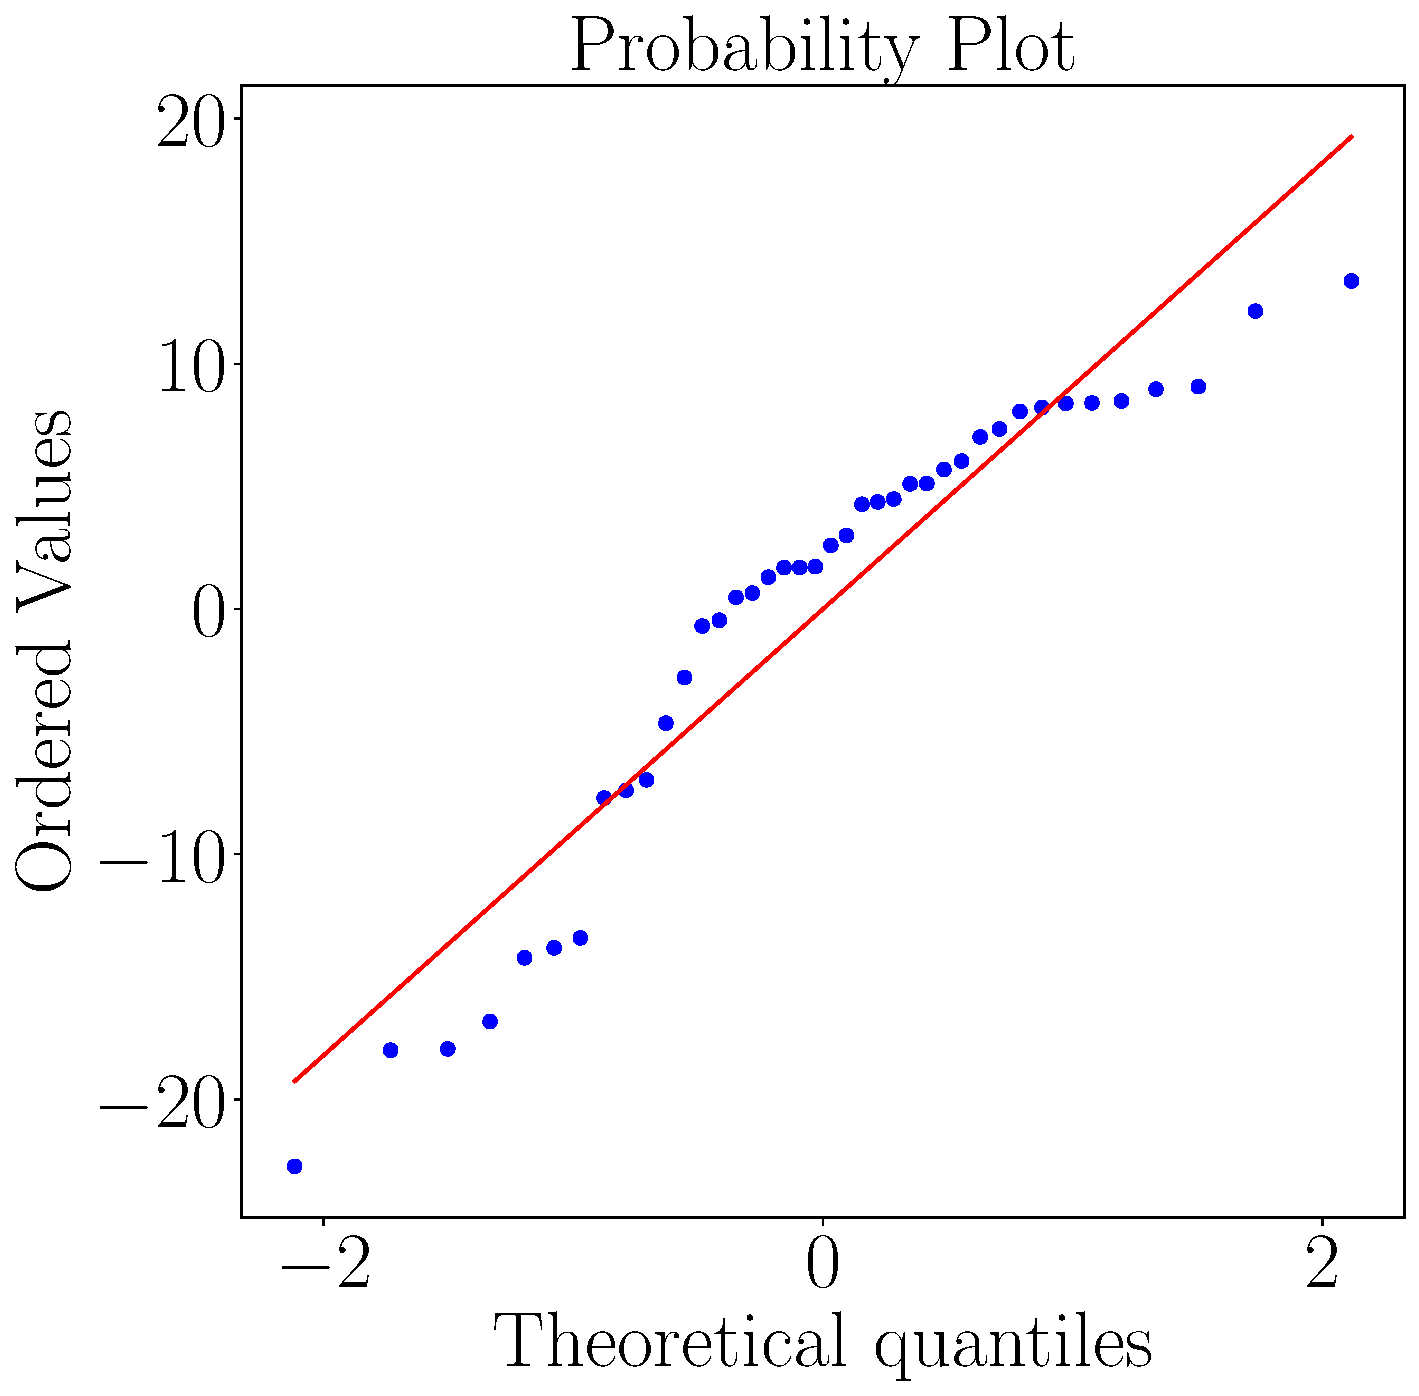
\includegraphics[width = \textwidth]{Resultados/ECG/Figuras/pdf/qqplot_bpm_two_way_blind.pdf}
        \caption{QQ plot of the BPM of the blind participants on each method.}
        \label{fig:qqplot_bpm_two_way_blind}
    \end{minipage}
    \begin{minipage}{0.075\textwidth}
        \hfill
    \end{minipage}
    \begin{minipage}{0.45\textwidth}
        \centering
        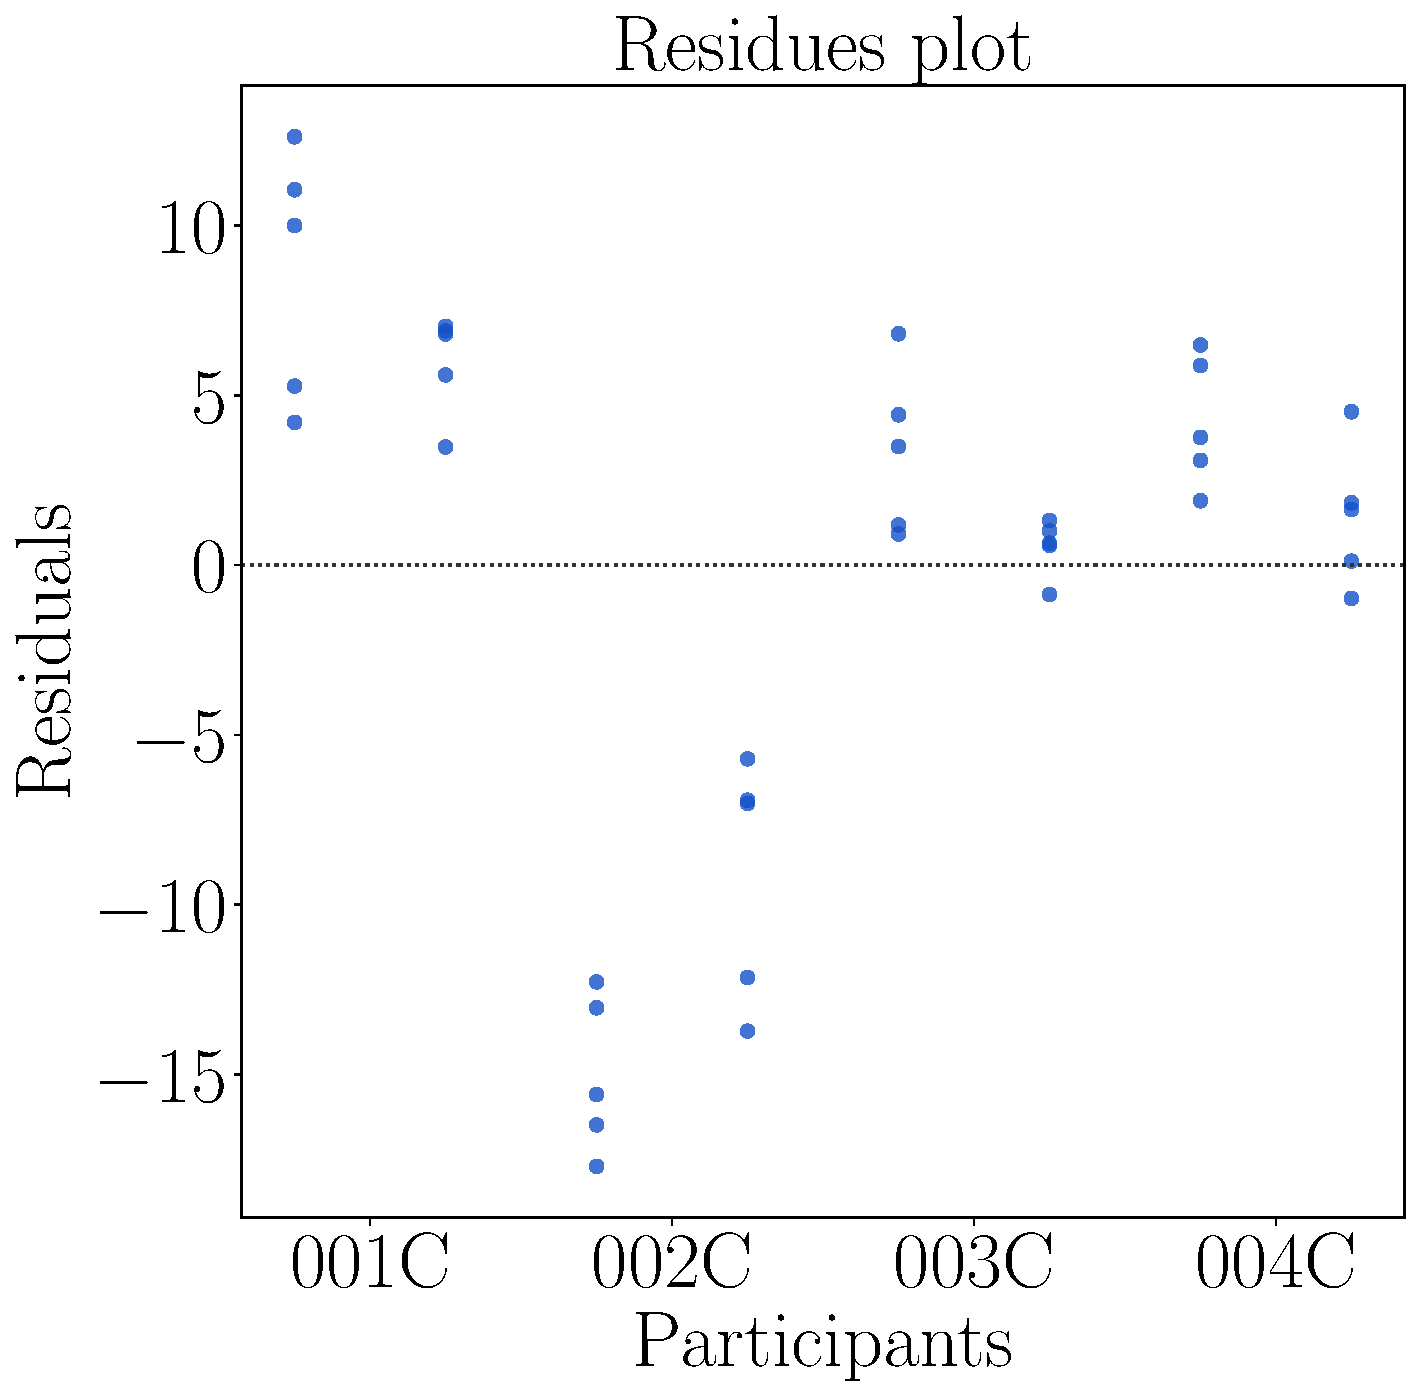
\includegraphics[width = \textwidth]{Resultados/ECG/Figuras/pdf/residplot_bpm_two_way_blind.pdf}
        \caption{Residual plot of the BPM score the blind participants on each method.}
        \label{fig:residplot_bpm_two_way_blind}
    \end{minipage}
\end{figure}


\begin{table}[!htb]
\centering
\caption{Anova p-value for the BPM on each method for blinded users.}
\label{tab:blocanova_bpm_two_way_blind}
\begin{tabular}{lrrrrr}
\toprule
               Source &  Squared sum &  DOF & Squared average &      F & \begin{tabular}[c]{@{}l@{}}P-Value \\ $(F_{0} > F)$\end{tabular} \\
\midrule
Participants (Blocks) &     2807.274 &    3 &         935.758 & 49.361 &                                                                  \\
         \    Methods &      164.045 &    4 &          41.011 &  2.163 &                                                            0.100 \\
          \    Rounds &       15.693 &    1 &          15.693 &  0.828 &                                                            0.371 \\
     \    Interaction &       20.606 &    4 &           5.152 &  0.272 &                                                            0.894 \\
   Experimental Error &      511.853 &   27 &          18.958 &        &                                                                  \\
                Total &     3519.471 &   39 &                 &        &                                                                  \\
\bottomrule
\end{tabular}
\end{table}



%
\begin{table}[!htb]
\centering
\caption{Cross validation p-value for the average BPM on each method for blinded users.}
\label{tab:lsd_bpm_two_way}
\begin{tabular}{rclr}
\toprule
      \multicolumn{3}{c}{Method} &                                           Analysis \\
\midrule
              Base & $X$ & Audio &               $H_1 : \mu_{Base} \ne \mu_{Audio}**$ \\
        Base & $X$ & Haptic Belt &             $H_0 : \mu_{Base} = \mu_{Haptic Belt}$ \\
       Base & $X$ & Virtual Cane &        $H_1 : \mu_{Base} \ne \mu_{Virtual Cane}**$ \\
            Base & $X$ & Mixture &             $H_1 : \mu_{Base} \ne \mu_{Mixture}**$ \\
       Audio & $X$ & Haptic Belt &        $H_1 : \mu_{Audio} \ne \mu_{Haptic Belt}**$ \\
      Audio & $X$ & Virtual Cane &       $H_1 : \mu_{Audio} \ne \mu_{Virtual Cane}**$ \\
           Audio & $X$ & Mixture &            $H_1 : \mu_{Audio} \ne \mu_{Mixture}**$ \\
Haptic Belt & $X$ & Virtual Cane & $H_1 : \mu_{Haptic Belt} \ne \mu_{Virtual Cane}**$ \\
     Haptic Belt & $X$ & Mixture &      $H_1 : \mu_{Haptic Belt} \ne \mu_{Mixture}**$ \\
    Virtual Cane & $X$ & Mixture &     $H_1 : \mu_{Virtual Cane} \ne \mu_{Mixture}**$ \\
\bottomrule
\end{tabular}
\end{table}



%The Table \ref{tab:lsd_bpm_two_way} presents the conclusion of a pairwise Fisher LSD test of the blind heart rate frequency variation between all the guidance methods. The results show that the only the Base and haptic belt have simila reaction.

%\FloatBarrier

%%%%%%%%%%%%%%%%%%%%%%%%%%%%%%%%%%%%%%%%%%%%%%%%%%%%%%%%%%%%%%%%%%%%%%%%%%%%
%%%%%%%%%%%%%%%%%%%%%%%%%%%%%%%%%%%%%%%%%%%%%%%%%%%%%%%%%%%%%%%%%%%%%%%%%%%%
%%%%%%%%%%%%%%%%%%%%%%%%%%%%%%%%%%%%%%%%%%%%%%%%%%%%%%%%%%%%%%%%%%%%%%%%%%%%
%%%%%%%%%%%%%%%%%%%%%%%%%%%%%%%%%%%%%%%%%%%%%%%%%%%%%%%%%%%%%%%%%%%%%%%%%%%%
%
%
\paragraph{Analysis of the heartbeat variance (SDNN)}\mbox{}\\
%
Table \ref{tab:sdnn_table_blind} brings the value of the second variable extracted from the ECG: SDNN, the standard deviation of the interbeat interval. Different to the heartrate frequency, if the variation between the First and the Return round is negative, it means that the user had an increase on his/her mental workload and vice-versa. Similar to what is observed for the BPM, it is not possible to draw a pattern from this data. The participants had increased or decreased their heartrate with different methods.


\begin{table}[!htb]
\centering
\caption{Average SDNN of the blind participants during the each round and method [ms].}
\label{tab:sdnn_table_blind}
\begin{tabular}{llrrrrr}
\toprule
     &        &    Base &   Audio &  \begin{tabular}[c]{@{}l@{}}Haptic\\ Belt\end{tabular} &  \begin{tabular}[c]{@{}l@{}}Virtual\\ Cane\end{tabular} &  Mixture \\
Participant & Round &         &         &                                                        &                                                         &          \\
\midrule
001C & First &  81.292 & 107.061 &                                                124.737 &                                                 163.968 &  129.054 \\
     & Return & 120.719 & 130.885 &                                                131.590 &                                                 157.589 &  124.786 \\
002C & First &  73.761 &  98.863 &                                                 81.140 &                                                  33.977 &   79.289 \\
     & Return & 108.940 &  49.627 &                                                 42.815 &                                                 114.057 &  107.545 \\
003C & First &  36.870 &  38.325 &                                                 35.101 &                                                  42.392 &   43.692 \\
     & Return &  52.750 &  41.196 &                                                 44.256 &                                                  42.602 &   46.145 \\
004C & First &  70.728 &  86.827 &                                                 62.560 &                                                  85.900 &   70.472 \\
     & Return &  71.950 &  74.895 &                                                 70.017 &                                                  66.089 &  104.040 \\
\bottomrule
\end{tabular}
\end{table}



The barplot of Figure \ref{fig:barplot_ecg_sdnn_5_scene_blind} shows the average SDNN for each method. It is possible to notice that some methods are associated with an increase in the SDNN between the rounds, while others present a slight decrease.

\begin{figure}[!htb]
    \centering
    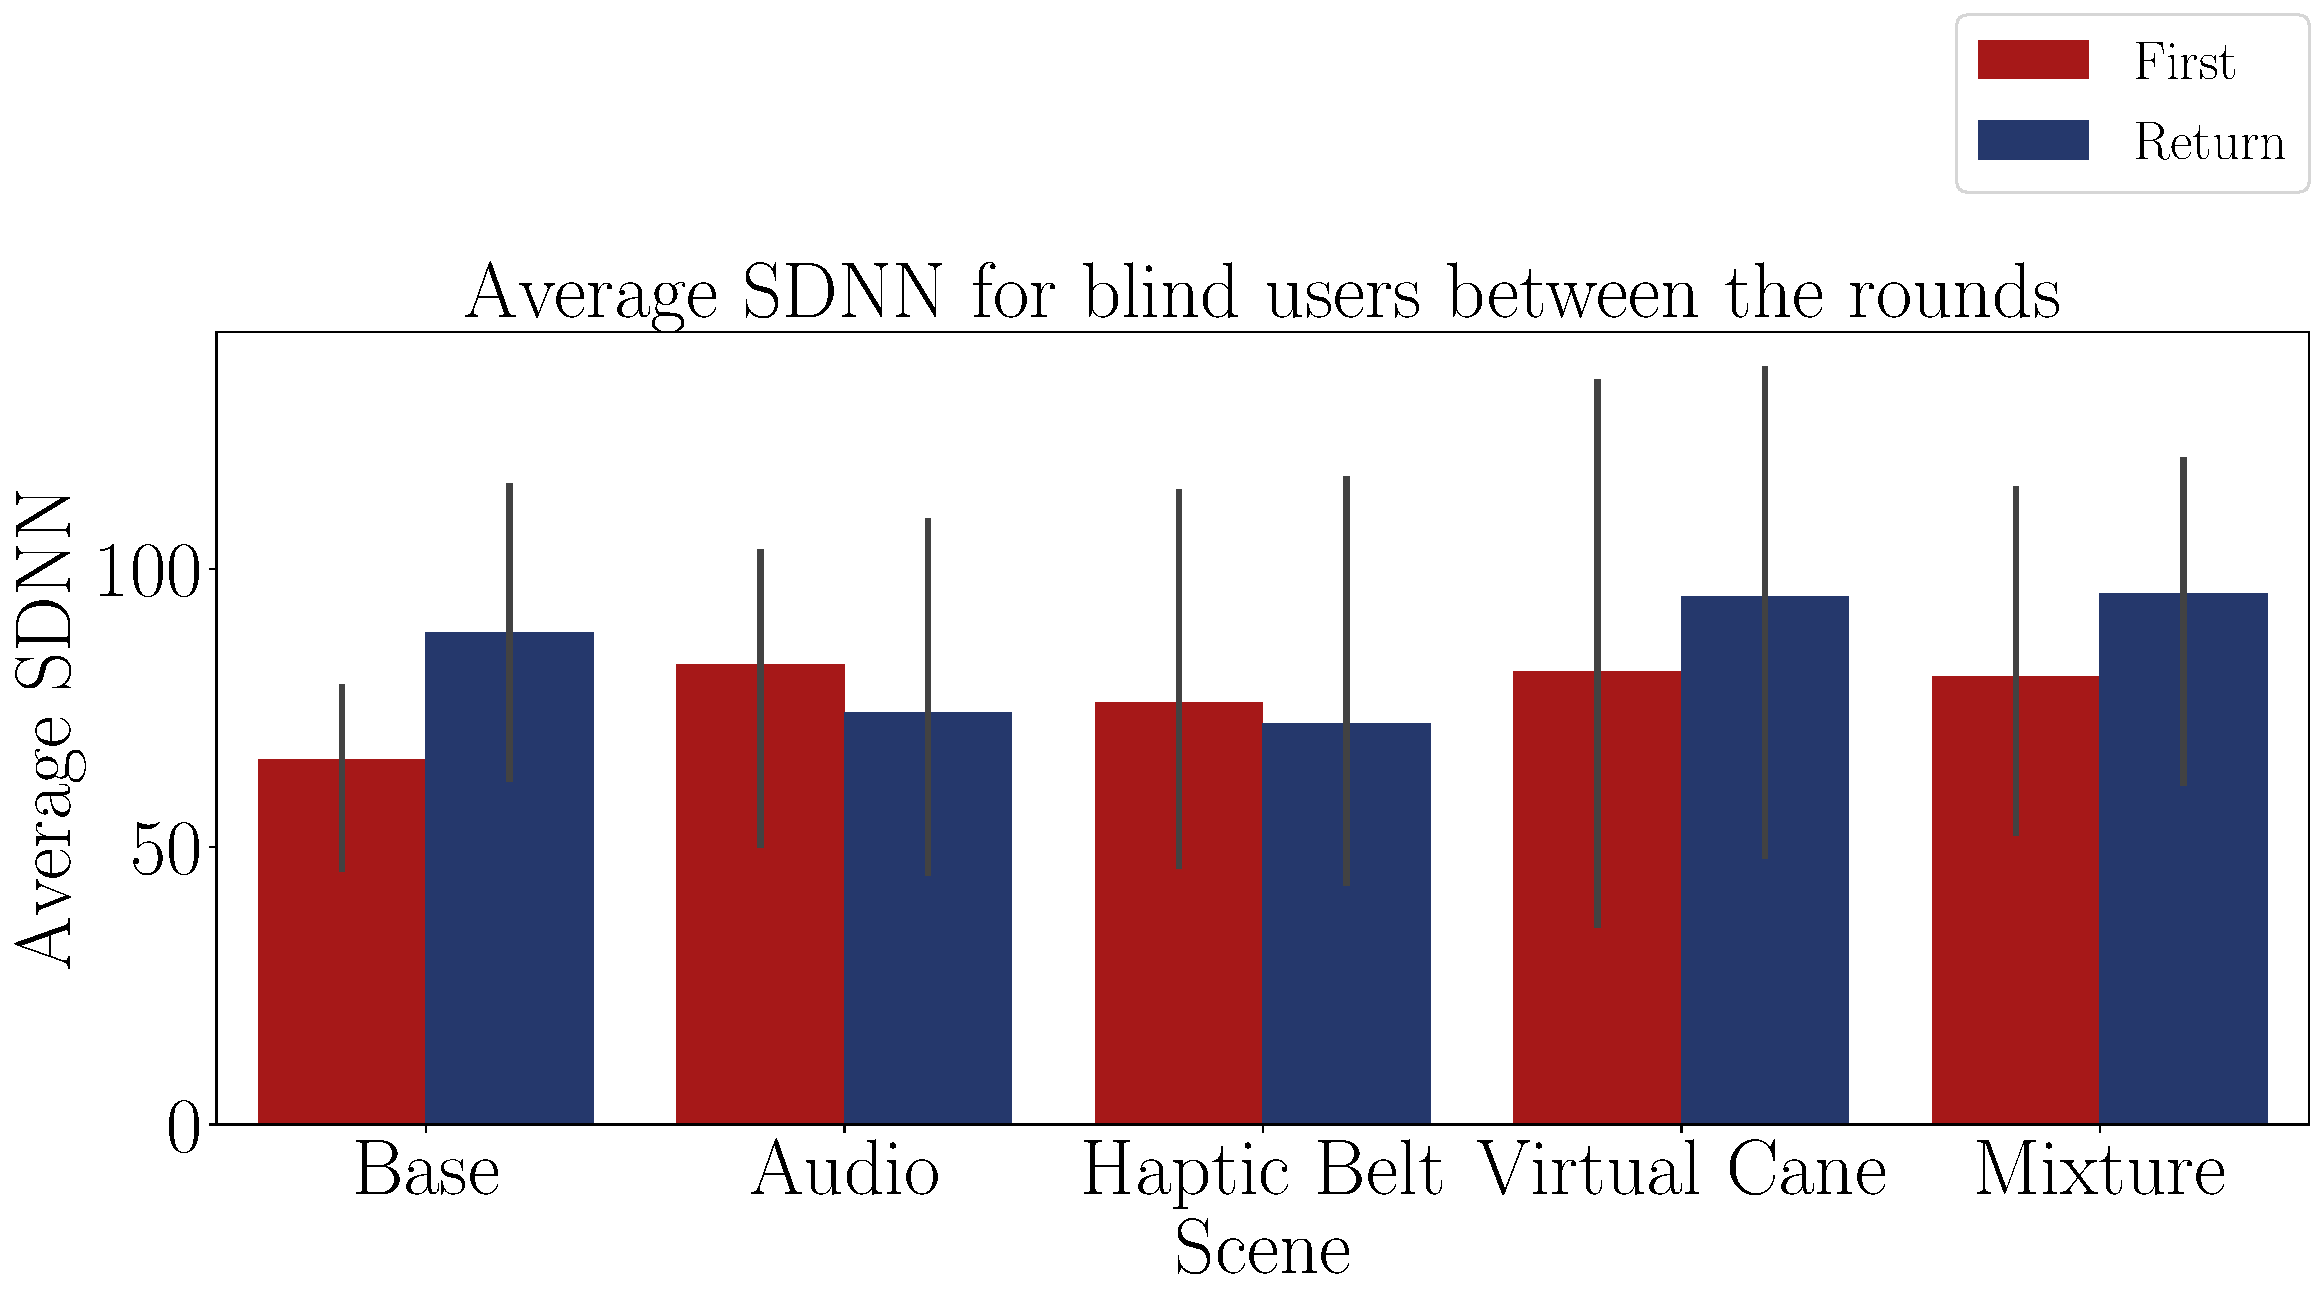
\includegraphics[width = \textwidth]{Resultados/ECG/Figuras/pdf/barplot_ecg_sdnn_5_scene_blind.pdf}
    \caption{Barplot of the average SDNN of the blind participants on each method.}
    \label{fig:barplot_ecg_sdnn_5_scene_blind}
\end{figure}

%The Table \ref{tab:sdnn_average_group_blind} presents the average SDNN variation between the rounds. It shows that only the audio and the haptic belt methods shown a increase in the mental workload.
%
%
\begin{table}[!htb]
\centering
\caption{ECG average SDNN for each method of the blind participants.}
\label{tab:sdnn_average_group_blind}
\begin{tabular}{lrrrrr}
\toprule
{} &   Base &  Audio & Haptic Belt & Virtual Cane & Mixture \\
Visual Condition &        &        &             &              &         \\
\midrule
Blind            &  77.13 &  78.46 &       74.03 &        88.32 &   88.13 \\
\bottomrule
\end{tabular}
\end{table}



Figure \ref{fig:boxplot_ecg_sdnn_blind_scene} and Figure \ref{fig:boxplot_ecg_sdnn_blind_rounds} bring the SDNN barplot grouped by the methods and the rounds. There is a slight tendency among the participants to increase the heartbeat in the return round.

\begin{figure}[!htb]
    \centering
    \begin{minipage}{0.45\textwidth}
        \centering
        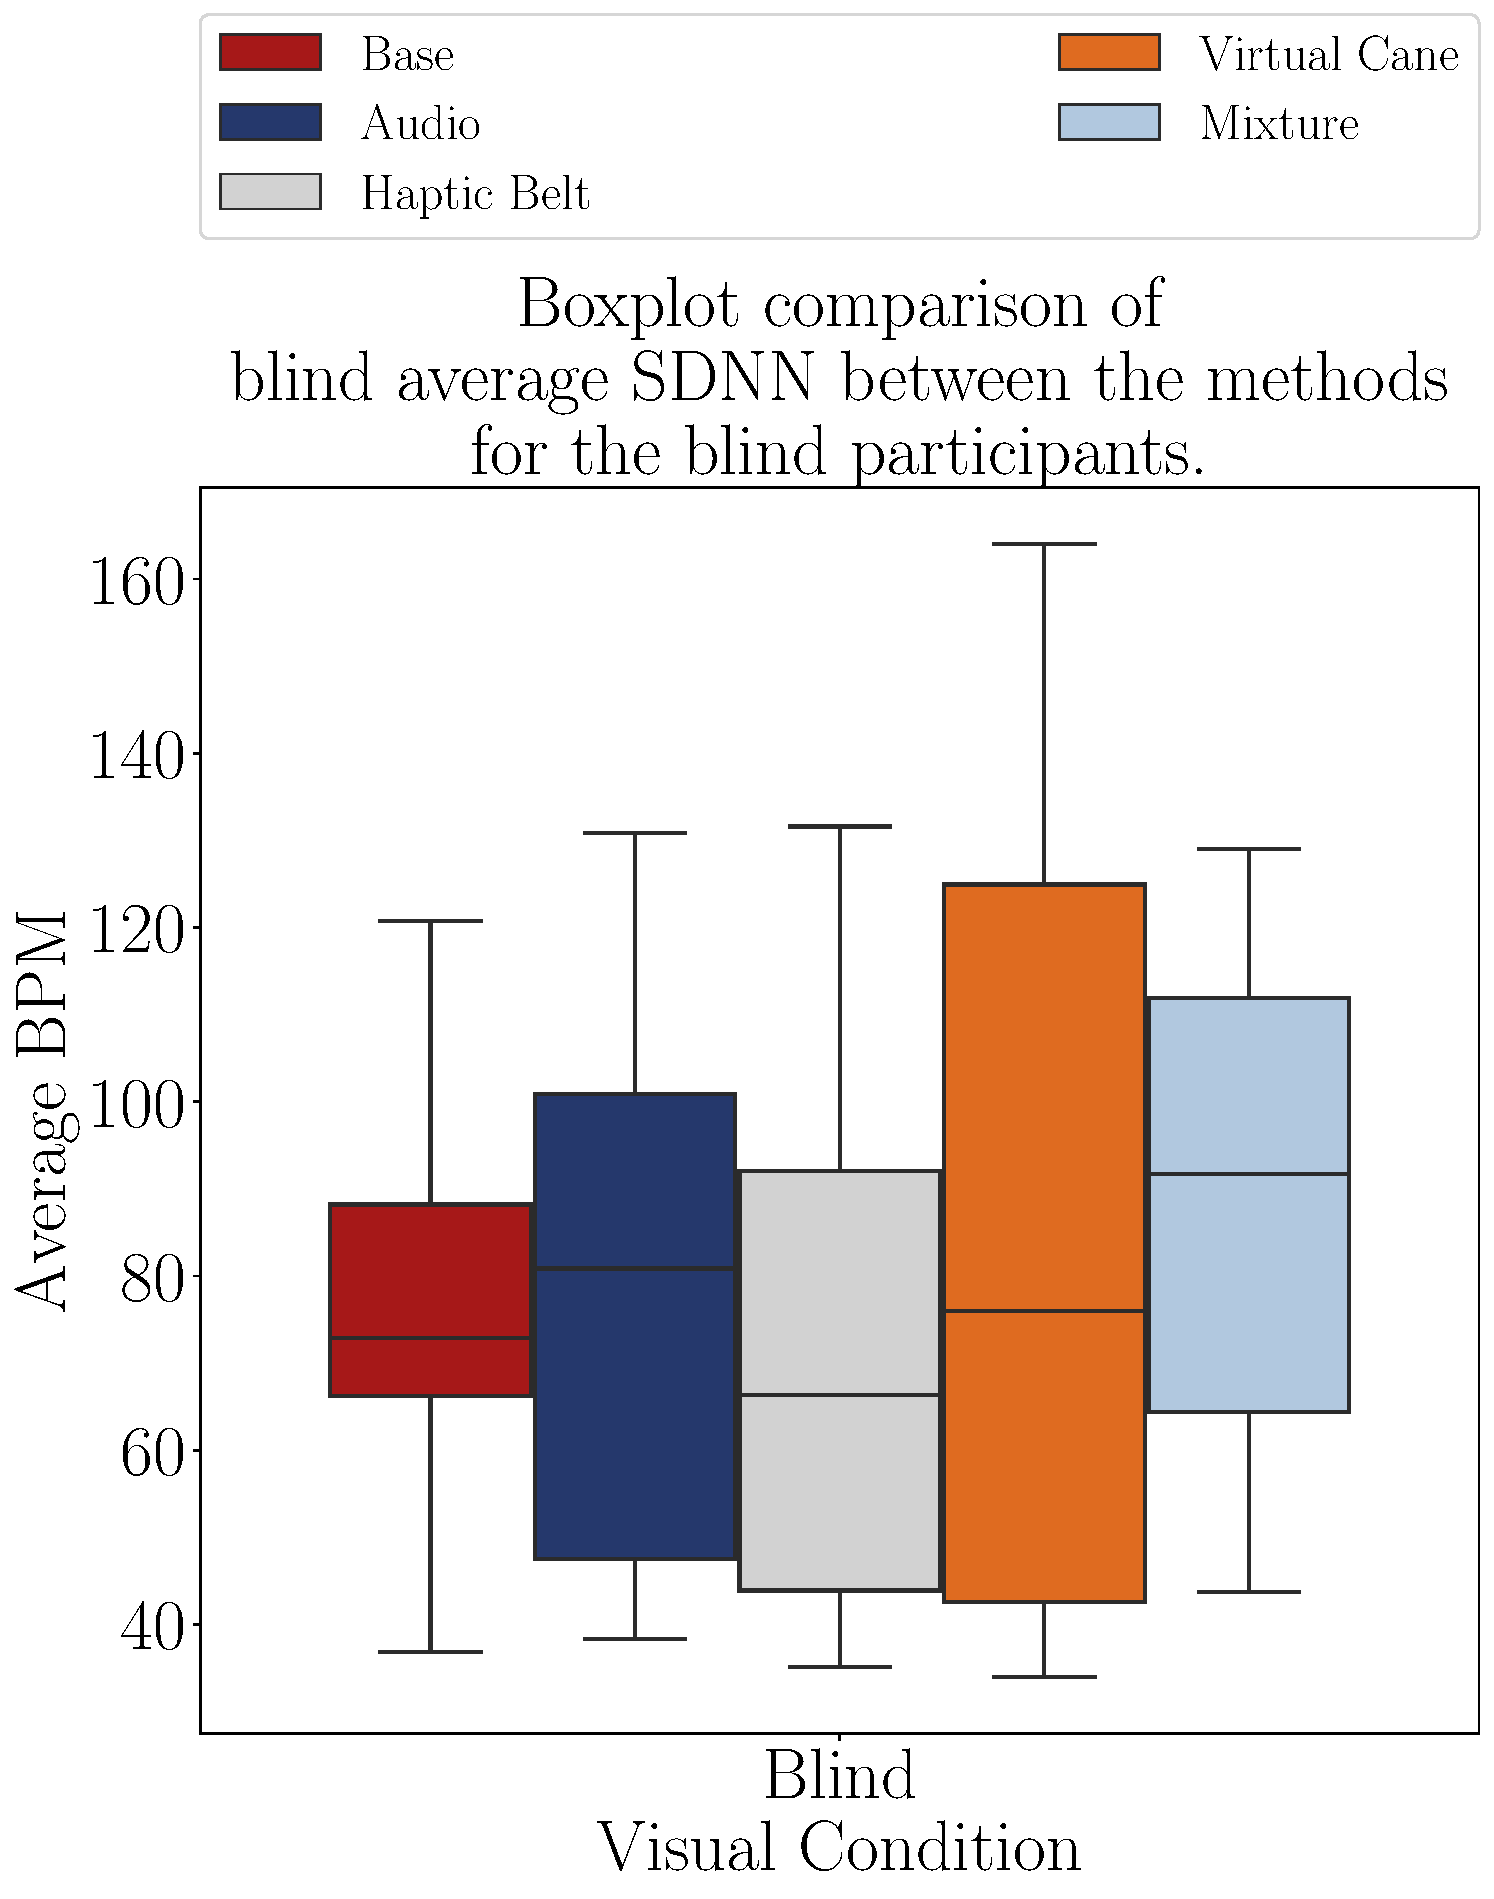
\includegraphics[width = \textwidth]{Resultados/ECG/Figuras/pdf/boxplot_ecg_sdnn_blind_scene.pdf}
        \caption{Boxplot of the SDNN of the blind participants grouped by the methods.}
        \label{fig:boxplot_ecg_sdnn_blind_scene}
    \end{minipage}
    \begin{minipage}{0.075\textwidth}
        \hfill
    \end{minipage}
    \begin{minipage}{0.45\textwidth}
        \centering
        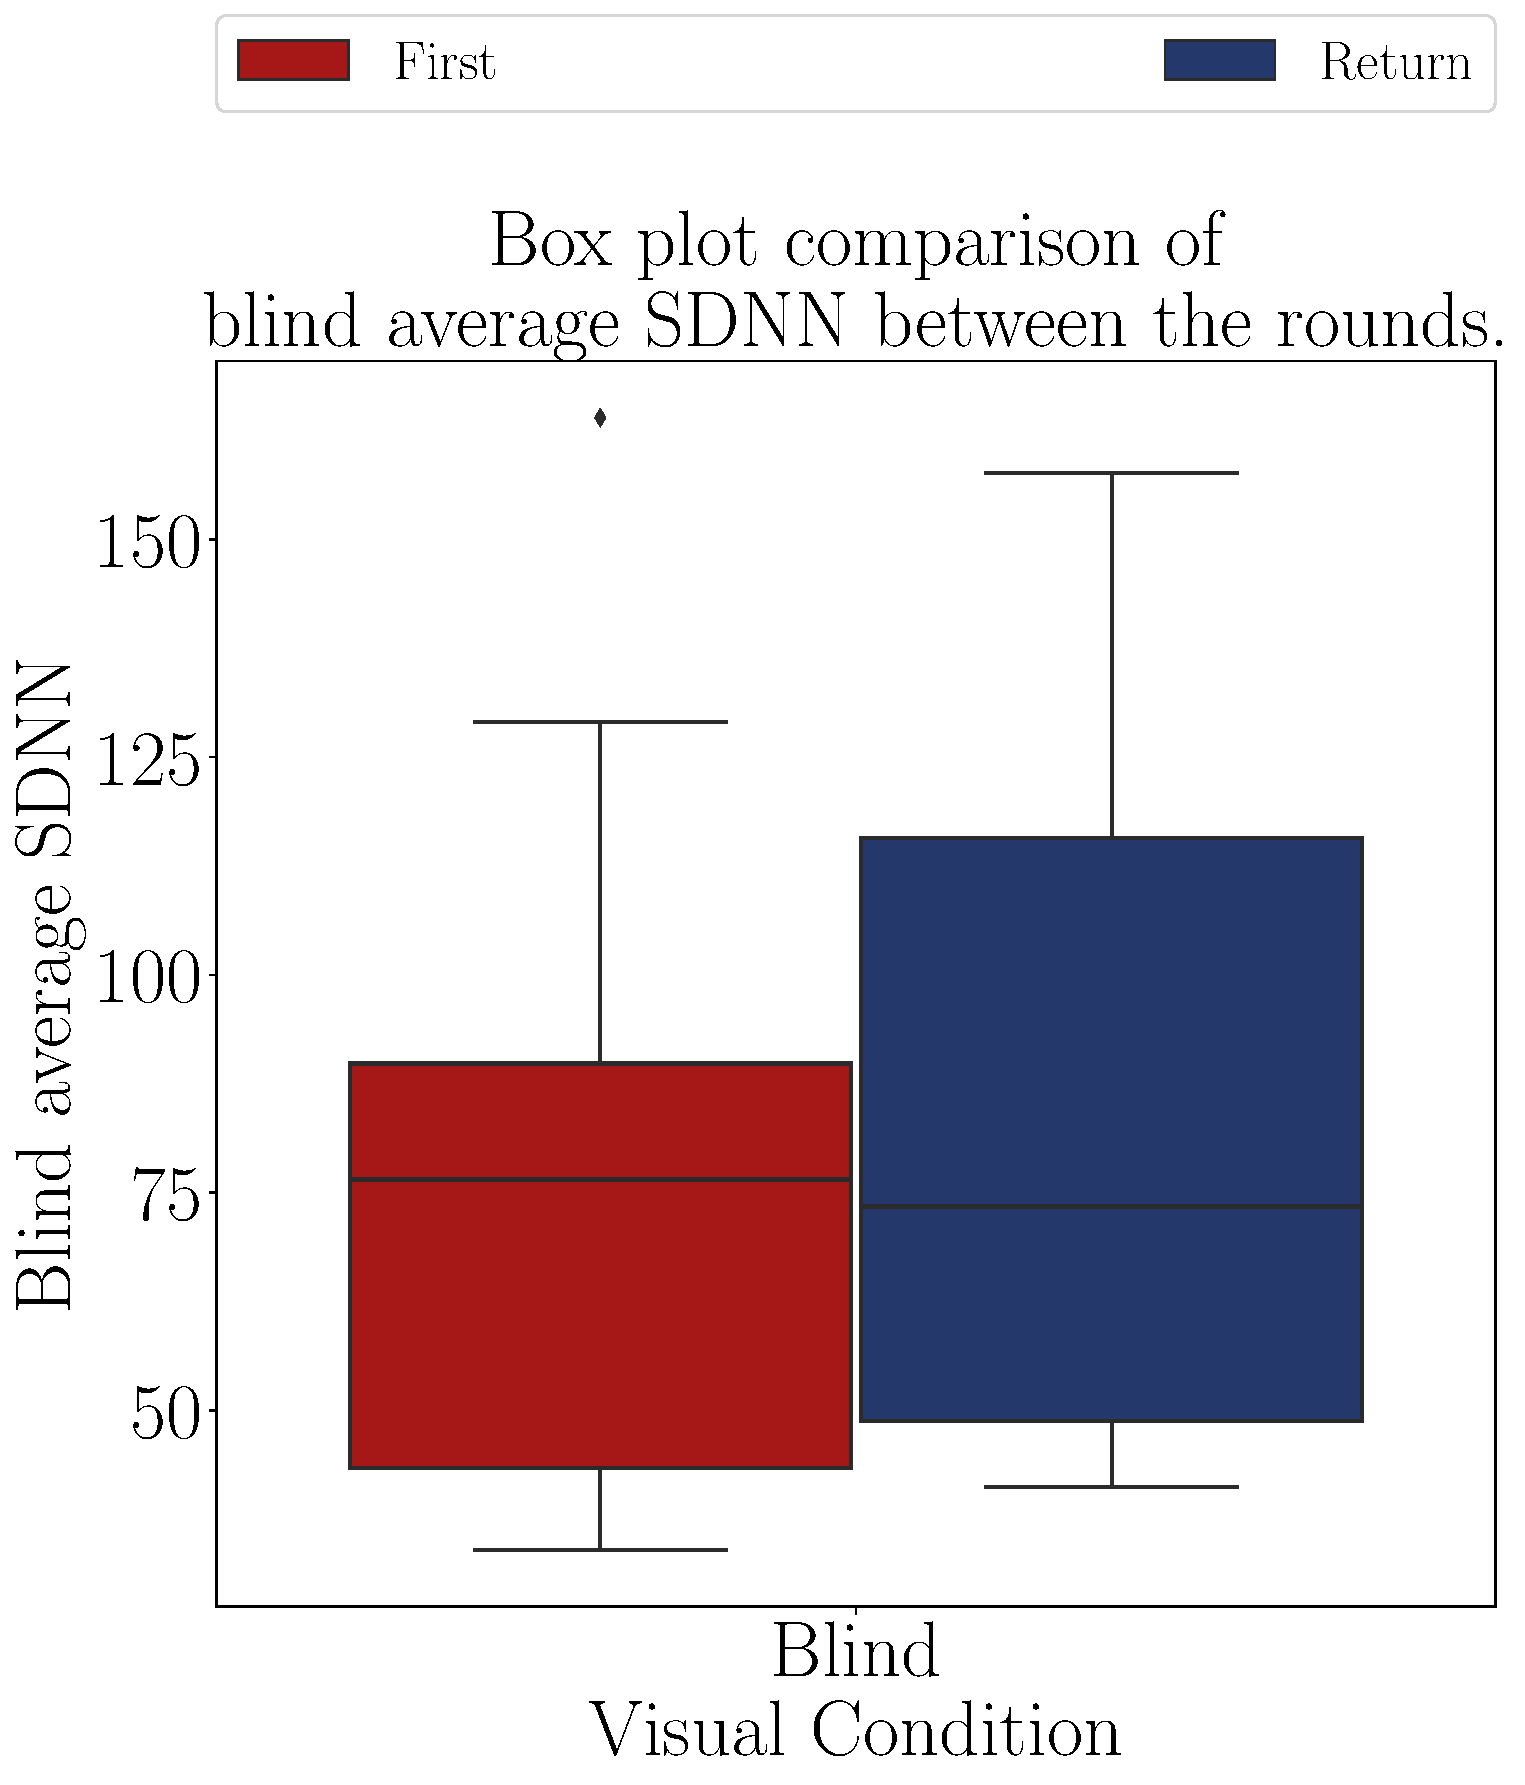
\includegraphics[width = \textwidth]{Resultados/ECG/Figuras/pdf/boxplot_ecg_sdnn_blind_rounds.pdf}
        \caption{Boxplot of the SDNN of the blind participants grouped by the rounds.}
        \label{fig:boxplot_ecg_sdnn_blind_rounds}
    \end{minipage}
\end{figure}


Figures \ref{fig:qqplot_sdnn_two_way_blind} and \ref{fig:residplot_sdnn_two_way_blind} bring the QQ Plot and residual distribution. In this case, the residual distribution is more uniform than in Figure \ref{fig:residplot_bpm_two_way_blind}. The ANOVA results are presented in Table \ref{tab:blocdanova_sdnn_two_way_blind} and do not confirm any influence of the methods nor the rounds on the ECG heartrate variance.

\begin{figure}[!htb]
    \centering
    \begin{minipage}{0.45\textwidth}
        \centering
        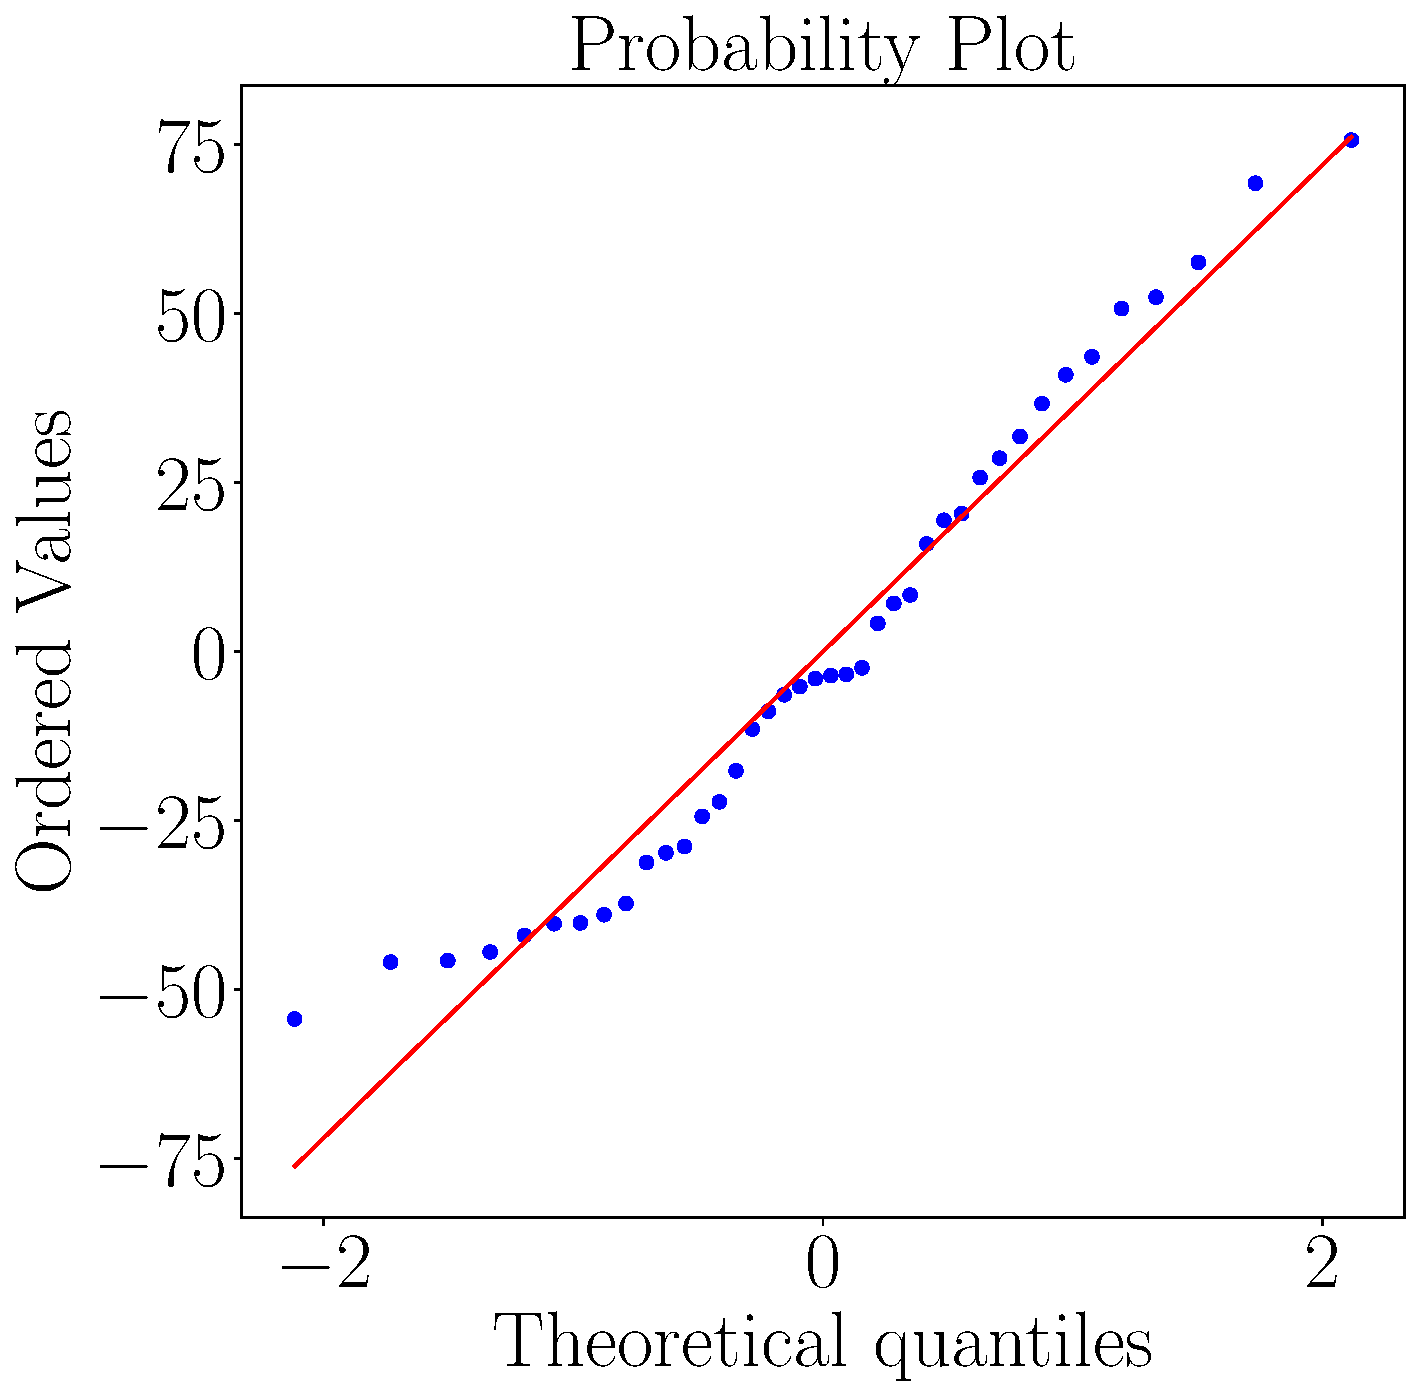
\includegraphics[width = \textwidth]{Resultados/ECG/Figuras/pdf/qqplot_sdnn_two_way_blind.pdf}
        \caption{QQ plot of the SDNN of the blind participants on each method.}
        \label{fig:qqplot_sdnn_two_way_blind}
    \end{minipage}
    \begin{minipage}{0.075\textwidth}
        \hfill
    \end{minipage}
    \begin{minipage}{0.45\textwidth}
        \centering
        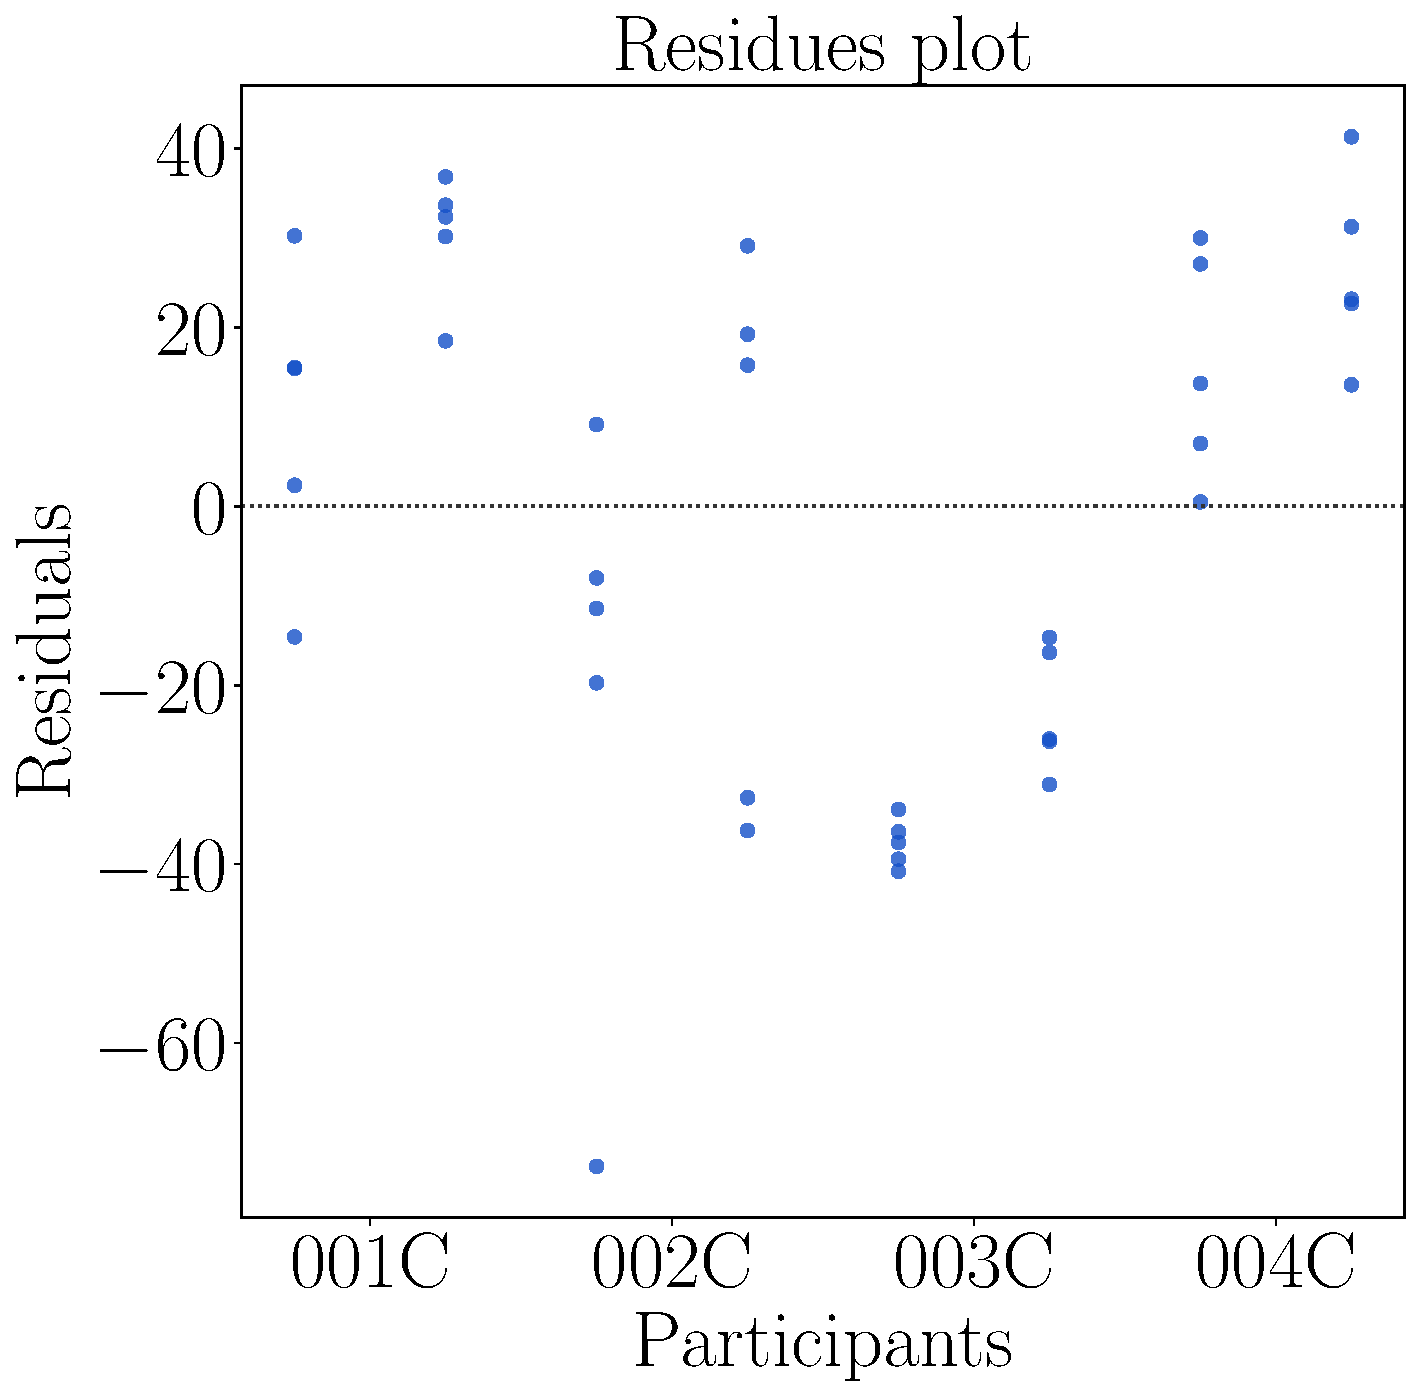
\includegraphics[width = \textwidth]{Resultados/ECG/Figuras/pdf/residplot_sdnn_two_way_blind.pdf}
        \caption{Residual plot of the SDNN of the blind participants on each method.}
        \label{fig:residplot_sdnn_two_way_blind}
    \end{minipage}
\end{figure}


\begin{table}[!htb]
\centering
\caption{Anova p-value for the average SDNN on each method for blinded users.}
\label{tab:blocdanova_sdnn_two_way_blind}
\begin{tabular}{lrrrrr}
\toprule
          Source & P-Value \\
\midrule
    \    Methods &   0.486 \\
     \    Rounds &   0.223 \\
\    Interaction &   0.473 \\
\bottomrule
\end{tabular}
\end{table}



\FloatBarrier
\subsubsection{Galvanic skin reaction and temperature data;}
\label{subsec:results_gsr_temp}

The GSR analysis is made by analyzing its average and the accumulated value and comparing both features between the baseline and each round. The temperature was analyzed with the GSR to see if there is some influence and by a graphical analysis there was none. For the experiment, the GSR sensor was worn on the left hand for right-handed participant and on the right hand for left-handed participants.

The Table \ref{tab:gsr_table_blind} presents the standard deviation of the interbeat interval by each participant on each scenes. As it was with the Table \ref{tab:bpm_table_blind}, it is not posible to draw a pattern inside this Table. Different participant had increase, or decrease, with different methods.


The Table \ref{tab:gsr_table_blind} presents the average skin conductance by each blind participant on their baseline and on each scene and their respectivily variation is inside Table \ref{tab:gsr_var_blind}. In the majority of times the skin conductance has risen from the "First" to the "Return" round, which mean that the participant was more aroused or with a higher mental workload.


\begin{table}[!htb]
\centering
\caption{Average GSR felled by the blind participants [$\mu$S].}
\label{tab:gsr_table_blind}
\begin{tabular}{lllrrrrrr}
\toprule
     &        & Baseline &  Base & Audio & \begin{tabular}[c]{@{}l@{}}Haptic\\ Belt\end{tabular} & \begin{tabular}[c]{@{}l@{}}Virtual\\ Cane\end{tabular} & Mixture \\
Participant & Round &          &       &       &                                                       &                                                        &         \\
\midrule
001C & First &     0.37 &  0.48 &  1.03 &                                                  3.14 &                                                   3.79 &    3.90 \\
     & Return &          &  0.83 &  1.58 &                                                  2.81 &                                                   4.04 &    4.57 \\
003C & First &     0.30 &  0.56 &  0.56 &                                                  0.62 &                                                   0.85 &    1.09 \\
     & Return &          &  0.62 &  0.63 &                                                  0.65 &                                                   0.92 &    1.06 \\
004C & First &     1.24 &  2.34 &  3.07 &                                                  3.49 &                                                   2.28 &    2.23 \\
     & Return &          &  2.57 &  2.95 &                                                  3.20 &                                                   2.21 &    2.24 \\
\bottomrule
\end{tabular}
\end{table}




\begin{table}[!htb]
\centering
\caption{Average GSR variation in relation to the baseline in each round of the blind participants [$\mu$S].}
\label{tab:gsr_var_blind}
\begin{tabular}{lllrrrrrr}
\toprule
     &        &      Base &     Audio & \begin{tabular}[c]{@{}l@{}}Haptic\\ Belt\end{tabular} & \begin{tabular}[c]{@{}l@{}}Virtual\\ Cane\end{tabular} &    Mixture \\
Participant & Round &           &           &                                                       &                                                        &            \\
\midrule
001C & First &   30.58\% &  176.54\% &                                              746.10\% &                                               920.72\% &   951.71\% \\
     & Return &  125.29\% &  327.42\% &                                              656.99\% &                                               988.93\% &  1132.39\% \\
002C & First &  432.66\% &   32.26\% &                                               -0.00\% &                                                 0.00\% &     0.00\% \\
     & Return &  151.71\% &    1.67\% &                                               -5.10\% &                                                 0.00\% &     0.00\% \\
003C & First &   85.36\% &   84.23\% &                                              104.19\% &                                               182.35\% &   258.80\% \\
     & Return &  105.34\% &  109.23\% &                                              112.95\% &                                               202.35\% &   249.72\% \\
004C & First &   89.62\% &  148.53\% &                                              182.84\% &                                                84.33\% &    80.69\% \\
     & Return &  108.22\% &  138.64\% &                                              159.00\% &                                                78.73\% &    81.61\% \\
\bottomrule
\end{tabular}
\end{table}



The Figure \ref{fig:barplot_gsr_avg_5_scene_blind} presents the average GSR variation on each method and one can say that the presence of a haptic device causes an increase in the skin conductance, hence its mental workload. Also it is posible to realize that the average skin conductance of the blind participants had incresed between the "First" and "Return" round, with the exception of the "Base" method and the "Haptic Belt" method.

\begin{figure}[!htb]
    \centering
    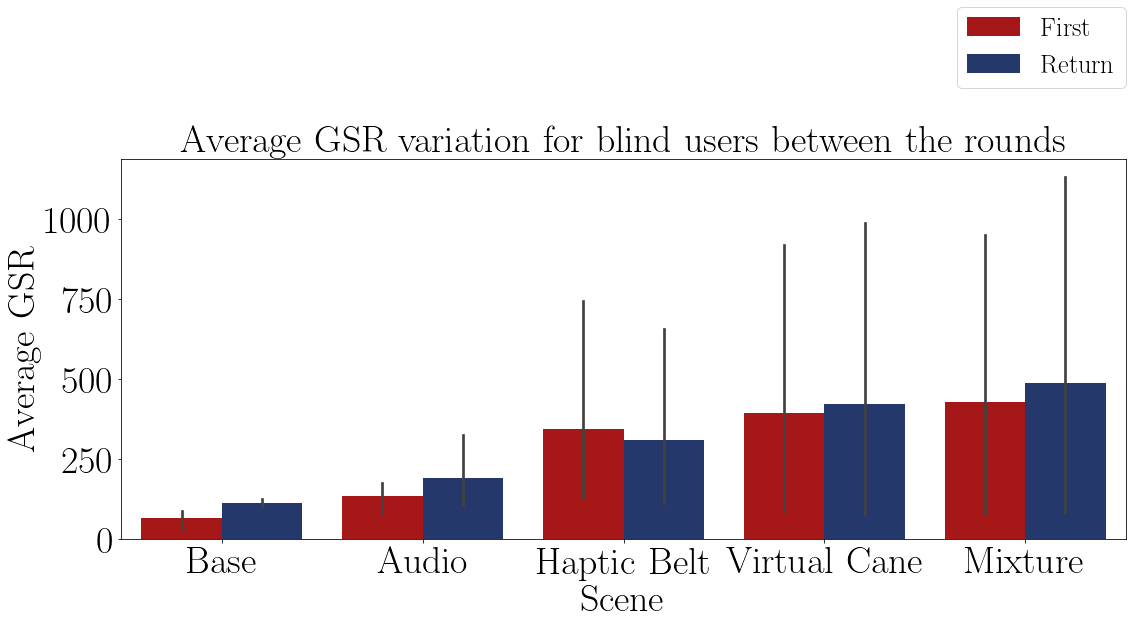
\includegraphics[width = 0.8\linewidth]{Resultados/GSR/Figuras/png/barplot_gsr_avg_5_scene_blind.png}
    \caption{Barplot of the average SDNN of the blind participants on each method.}
    \label{fig:barplot_gsr_avg_5_scene_blind}
\end{figure}

The Table \ref{tab:gsr_average_group_blind} presents the average GSR variation presented in the table \ref{tab:gsr_var_blind}. It shows that the "Audio" method presented the lesser GSR, that could be a combination of the fact that during the "Audio" method the hands was not used and that the participants felt less strange to the method, since it is based a common daily activity.


\begin{table}[!htb]
\centering
\caption{Average GSR variation by the blind participants}
\label{tab:gsr_average_group_blind}
\begin{tabular}{lrrrrr}
\toprule
{} &      Base &     Audio & \begin{tabular}[c]{@{}l@{}}Haptic\\ Belt\end{tabular} & \begin{tabular}[c]{@{}l@{}}Virtual\\ Cane\end{tabular} &  Mixture \\
Visual Condition &           &           &                                                       &                                                        &          \\
\midrule
Blind            &  141.10\% &  127.32\% &                                              244.62\% &                                               307.18\% &  344.366 \\
\bottomrule
\end{tabular}
\end{table}



The Figures \ref{fig:boxplot_gsr_avg_blind_scene} presents the distribution of the skin conductance on each method. It noticeable that the "Base" method has the lowest variation of all methods and that the presence of a haptic device increases its variance. The Figure \ref{fig:boxplot_gsr_avg_blind_rounds} presents the GSR grouped by the rounds and their are virtually the same.

\begin{figure}[!htb]
    \centering
    \begin{minipage}{0.45\textwidth}
        \centering
        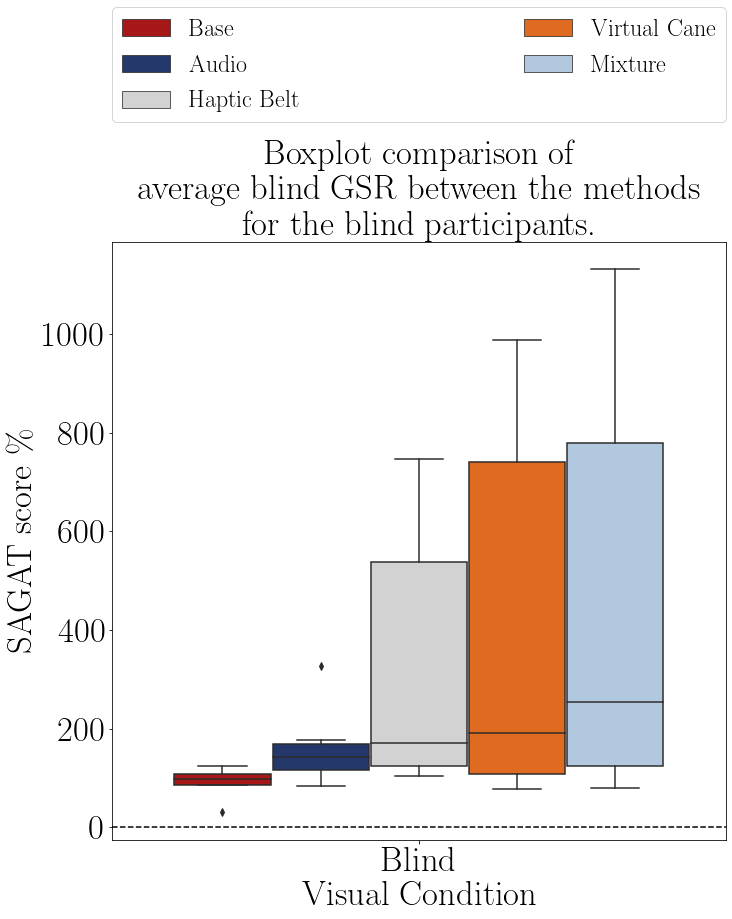
\includegraphics[width = 0.8\linewidth]{Resultados/GSR/Figuras/png/boxplot_gsr_avg_blind_scene.png}
        \caption{Boxplot of the GSR of the blind participants grouped by method.}
        \label{fig:boxplot_gsr_avg_blind_scene}
    \end{minipage}
    \begin{minipage}{0.45\textwidth}
        \centering
        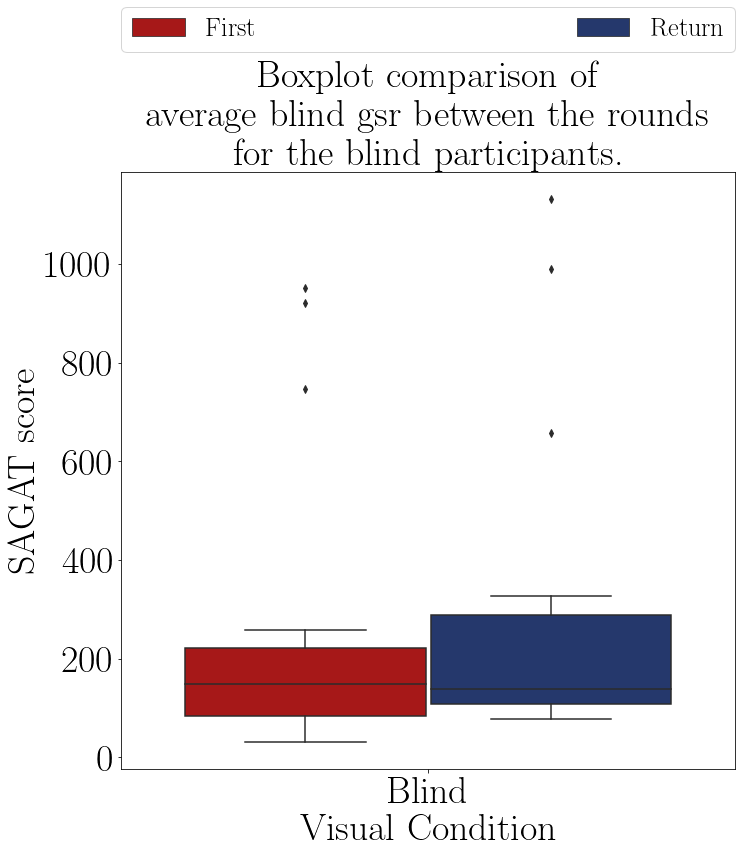
\includegraphics[width = 0.8\linewidth]{Resultados/GSR/Figuras/png/boxplot_gsr_avg_blind_rounds.png}
        \caption{Boxplot of the GSR of the blind participants grouped by round.}
        \label{fig:boxplot_gsr_avg_blind_rounds}
    \end{minipage}
\end{figure}

The Figures \ref{fig:qqplot_gsr_two_way} and \ref{fig:residplot_gsr_two_way} shows the distribution and variance of the Table \ref{tab:gsr_var_blind}. These Figures shows that the data are normally distributed but the participants had different  that the methods have a similar variance.
The Table \ref{tab:blocanova_gsr_two_way} shows the ANOVA test p-value of the heartbeat interval variance of the “blind” sample. The p-value indicates that there is no effect of any factor in the skin conductance.


\begin{table}[!htb]
\centering
\caption{Anova p-value for the mental demand average on each method for blinded users.}
\label{tab:blocanova_gsr_two_way}
\begin{tabular}{lrrrrl}
\toprule
               Source &  Squared sum &  DOF & Squared average &      F & \begin{tabular}[c]{@{}l@{}}P-Value \\ $(F_{0} > F)$\end{tabular} \\
\midrule
Participants (Blocks) &  1892069.020 &    3 &      630689.673 & 12.122 &                                                                  \\
         \    Methods &   301240.557 &    4 &       75310.139 &  1.447 &                                                            0.246 \\
          \    Rounds &      445.951 &    1 &         445.951 &  0.009 &                                                            0.927 \\
     \    Interaction &    10636.848 &    4 &        2659.212 &  0.051 &                                                            0.995 \\
   Experimental Error &  1404764.738 &   27 &       52028.324 &        &                                                                  \\
                Total &  3609157.113 &   39 &                 &        &                                                                  \\
\bottomrule
\end{tabular}
\end{table}



\begin{figure}[!htb]
    \centering
    \begin{minipage}{0.45\textwidth}
        \centering
        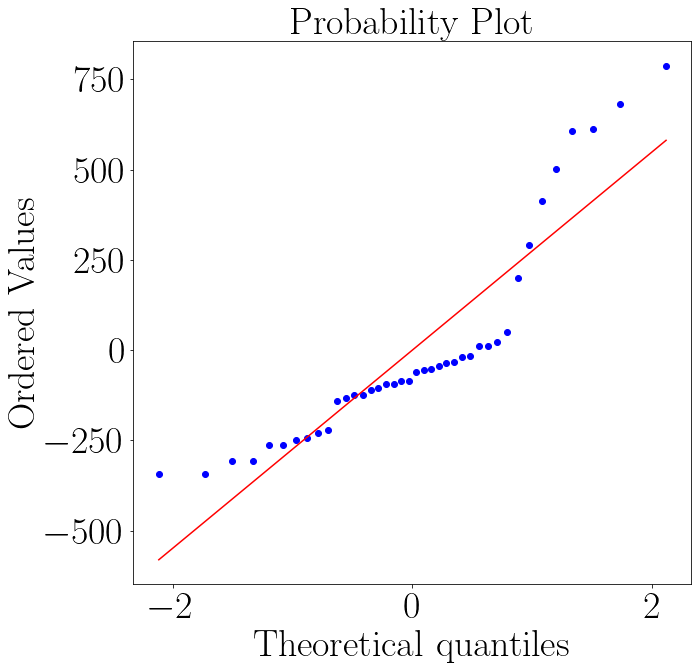
\includegraphics[width = 0.8\linewidth]{Resultados/GSR/Figuras/png/qqplot_gsr_two_way.png}
        \caption{QQ plot of the SDNN of the blind participants on each method.}
        \label{fig:qqplot_gsr_two_way}
    \end{minipage}
    \begin{minipage}{0.45\textwidth}
        \centering
        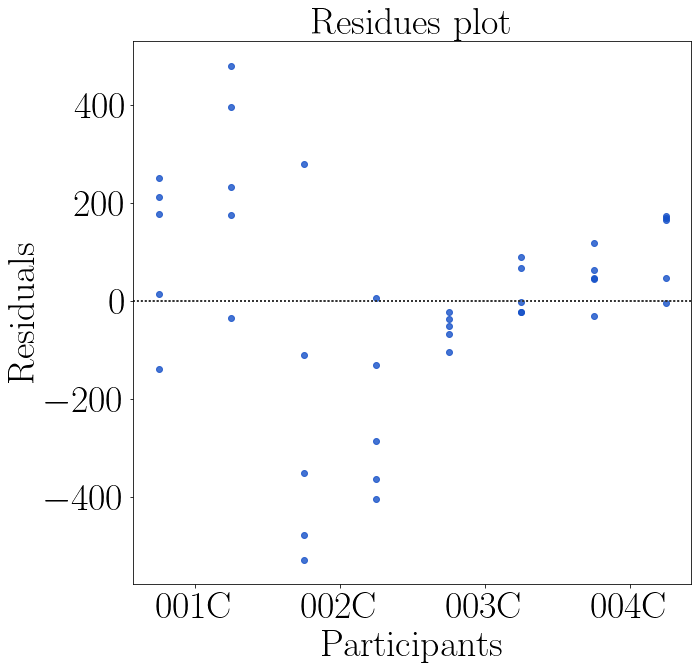
\includegraphics[width = 0.8\linewidth]{Resultados/GSR/Figuras/png/residplot_gsr_two_way.png}
        \caption{Residual plot of the SDNN of the blind participants on each method.}
        \label{fig:residplot_gsr_two_way}
    \end{minipage}
\end{figure}

%
\begin{table}[!htb]
\centering
\caption{Cross validation p-value for the mental demand average on each method for blinded users.}
\label{tab:lsd_gsr_two_way}
\begin{tabular}{rclr}
\toprule
      \multicolumn{3}{c}{Method} &                                           Analysis \\
\midrule
              Base & $X$ & Audio &                   $H_0 : \mu_{Base} = \mu_{Audio}$ \\
        Base & $X$ & Haptic Belt &         $H_1 : \mu_{Base} \ne \mu_{Haptic Belt}**$ \\
       Base & $X$ & Virtual Cane &        $H_1 : \mu_{Base} \ne \mu_{Virtual Cane}**$ \\
            Base & $X$ & Mixture &             $H_1 : \mu_{Base} \ne \mu_{Mixture}**$ \\
       Audio & $X$ & Haptic Belt &        $H_1 : \mu_{Audio} \ne \mu_{Haptic Belt}**$ \\
      Audio & $X$ & Virtual Cane &       $H_1 : \mu_{Audio} \ne \mu_{Virtual Cane}**$ \\
           Audio & $X$ & Mixture &            $H_1 : \mu_{Audio} \ne \mu_{Mixture}**$ \\
Haptic Belt & $X$ & Virtual Cane & $H_1 : \mu_{Haptic Belt} \ne \mu_{Virtual Cane}**$ \\
     Haptic Belt & $X$ & Mixture &      $H_1 : \mu_{Haptic Belt} \ne \mu_{Mixture}**$ \\
    Virtual Cane & $X$ & Mixture &         $H_0 : \mu_{Virtual Cane} = \mu_{Mixture}$ \\
\bottomrule
\end{tabular}
\end{table}



The Table \ref{tab:blocanova_gsr_two_way} does not prove that any method or round has some influence in the skin conductance variation, thus in the Mental Workload. Although, in the Figure \ref{fig:boxplot_gsr_avg_blind_scene} it is posible to notice that the "Base" and the "Audio" method have a different distribution. As it has already commented before, maybe the result of the anova test is a conseguence of a small sample size.

\FloatBarrier



\subsection{Final Remarks}

Summarizing the conclusion obtained from the analysis of the data from blind participants, the audio method showed a lower score both for NASA-TLX mental demand and NASA-TLX global score, while the methods that include vibration achieved higher scores. This probably happened because the participants are already used to use sound to guide themselves, especially environmental sounds. The environment sounds used in the scenes were always the same (telephone ringing, laptop keyboard sounds, exterior noise, door opening and closing). It is likely that the participants felt more relaxed when they only had to focus on the sounds around him/her. This is reinforced by the fact that, during experiment with the “audio” method, half of the participants did not ask for any information or the audio command option used only a few times.

The fact that the haptic devices caused a higher workload is probably due to the fact that the users had to learn and get used with them. Besides, for being just conceptual, their precision was not as good as they were expecting. That explains why their results were not as good as the “Base” or “Audio” methods. The NASA-TLX results are correctly related to the satisfaction questionnaires, which scored them as the unsatisfied devices.

As expected, most of the variables from subjective questionnaires (NASA-TLX and SAGAT) show some influence of the round, as expected. On the other hand, the results from the physiological sensors did not show clear tendency. 

The statistical analysis based on ANOVA tests confirmed some of the observations from the bar and box plots. However, in many cases the residual distributions were not homogenous and the statistical analysis was affected by the small number of samples. 

All the blind participants showed a great enthusiasm before, during and after the experiment. They also made a number of recommendations for both the virtual environment and the devices, such as:

\begin{itemize}
    \item The speakers of the HMD are not good enough to give them the precise location of the sound origin
    \item The HMD is too large and cover half of the participant’s face. It gives them a strange sensation, since some of them use the air or the wind feeling on the face to give them hints about the location of walls or other high obstacles;
    \item The precision of the vibration for both haptic belt and virtual cane needs to be improved. It is not enough for them to use the devices. This problem is related to how the HMD set the position of the user in the virtual environment. \\    
    \item The vibration from the haptic belt was not intense enough.
\end{itemize}

\section{Comparison between BVI users and sighted users}
\label{sec:results_obj_2}

This section is dedicated to investigate the second research question of this work: “do non-BVI users, when deprived from their vision, evaluate assistive devices in a similar way as BVI users?”. 

In order to do so, the analysis performed in the previous section is now repeated with the data obtained from sighted participants. However, the data corresponding to the ‘base’ method is omitted, as the daily method used by sighted people is based on their vision.

%\subsection{Subjective data}

Only two of the questionnaires will be analyzed, the NASA-TLX and the Adapted SAGAT, and it is expected that for:

\begin{itemize}
    \item \nameref{subsubsec:results_nasa_tlx_2};
    
        There will be a noticeable difference between the sight sample mental workload and the blind sample mental workload.

    \item \nameref{subsubsec:results_adapted_sagat_2};
    
        Is expected to notice a difference between the “blind” sample and the “sight” sample.

\end{itemize}

\subsubsection{NASA-TLX}
\label{subsubsec:results_nasa_tlx_2}

\paragraph{Analysis of the mental demand scale}\mbox{}\\

The Table \ref{tab:md_table_noBase} presents the ‘mental demand’ score of all participants, while the corresponding barplot is presented in Figure \ref{fig:barplot_md_avg_4_scene_blind_sight}. It is interesting to observe that sighted people gave a higher score to audio, as they are not so familiar to use sounds as source of guidance.


\begin{table}[!htb]
\centering
\caption{Mental demand felled by the participants.}
\label{tab:md_table_noBase}
\begin{tabular}{lllrrrrr}
\toprule
    &       &        & Audio & \begin{tabular}[c]{@{}l@{}}Haptic\\ Belt\end{tabular} & \begin{tabular}[c]{@{}l@{}}Virtual\\ Cane\end{tabular} & Mixture \\
Participant & \begin{tabular}[c]{@{}l@{}}Visual\\ Condition\end{tabular} & Round &       &                                                       &                                                        &         \\
\midrule
001 & Sight & First &    12 &                                                    11 &                                                      5 &       9 \\
    &       & Return &    13 &                                                    13 &                                                      5 &      10 \\
001C & Blind & First &     1 &                                                    14 &                                                      3 &       6 \\
    &       & Return &     1 &                                                    10 &                                                      2 &       6 \\
002C & Blind & First &     1 &                                                     1 &                                                     10 &      12 \\
    &       & Return &     1 &                                                     1 &                                                     10 &       3 \\
003 & Sight & First &    18 &                                                    18 &                                                     16 &      10 \\
    &       & Return &    12 &                                                    15 &                                                     11 &       8 \\
003C & Blind & First &     5 &                                                     5 &                                                      8 &       1 \\
    &       & Return &     1 &                                                     1 &                                                      2 &       1 \\
004 & Sight & First &    17 &                                                    20 &                                                     12 &      20 \\
    &       & Return &    12 &                                                    15 &                                                     10 &      15 \\
004C & Blind & First &    10 &                                                    15 &                                                     10 &      10 \\
    &       & Return &    10 &                                                    14 &                                                      8 &      10 \\
005 & Sight & First &     4 &                                                    12 &                                                     10 &      13 \\
    &       & Return &     6 &                                                    10 &                                                      6 &      12 \\
\bottomrule
\end{tabular}
\end{table}



\begin{figure}[!thb]
    \centering
    \begin{minipage}{\textwidth}
        \centering
        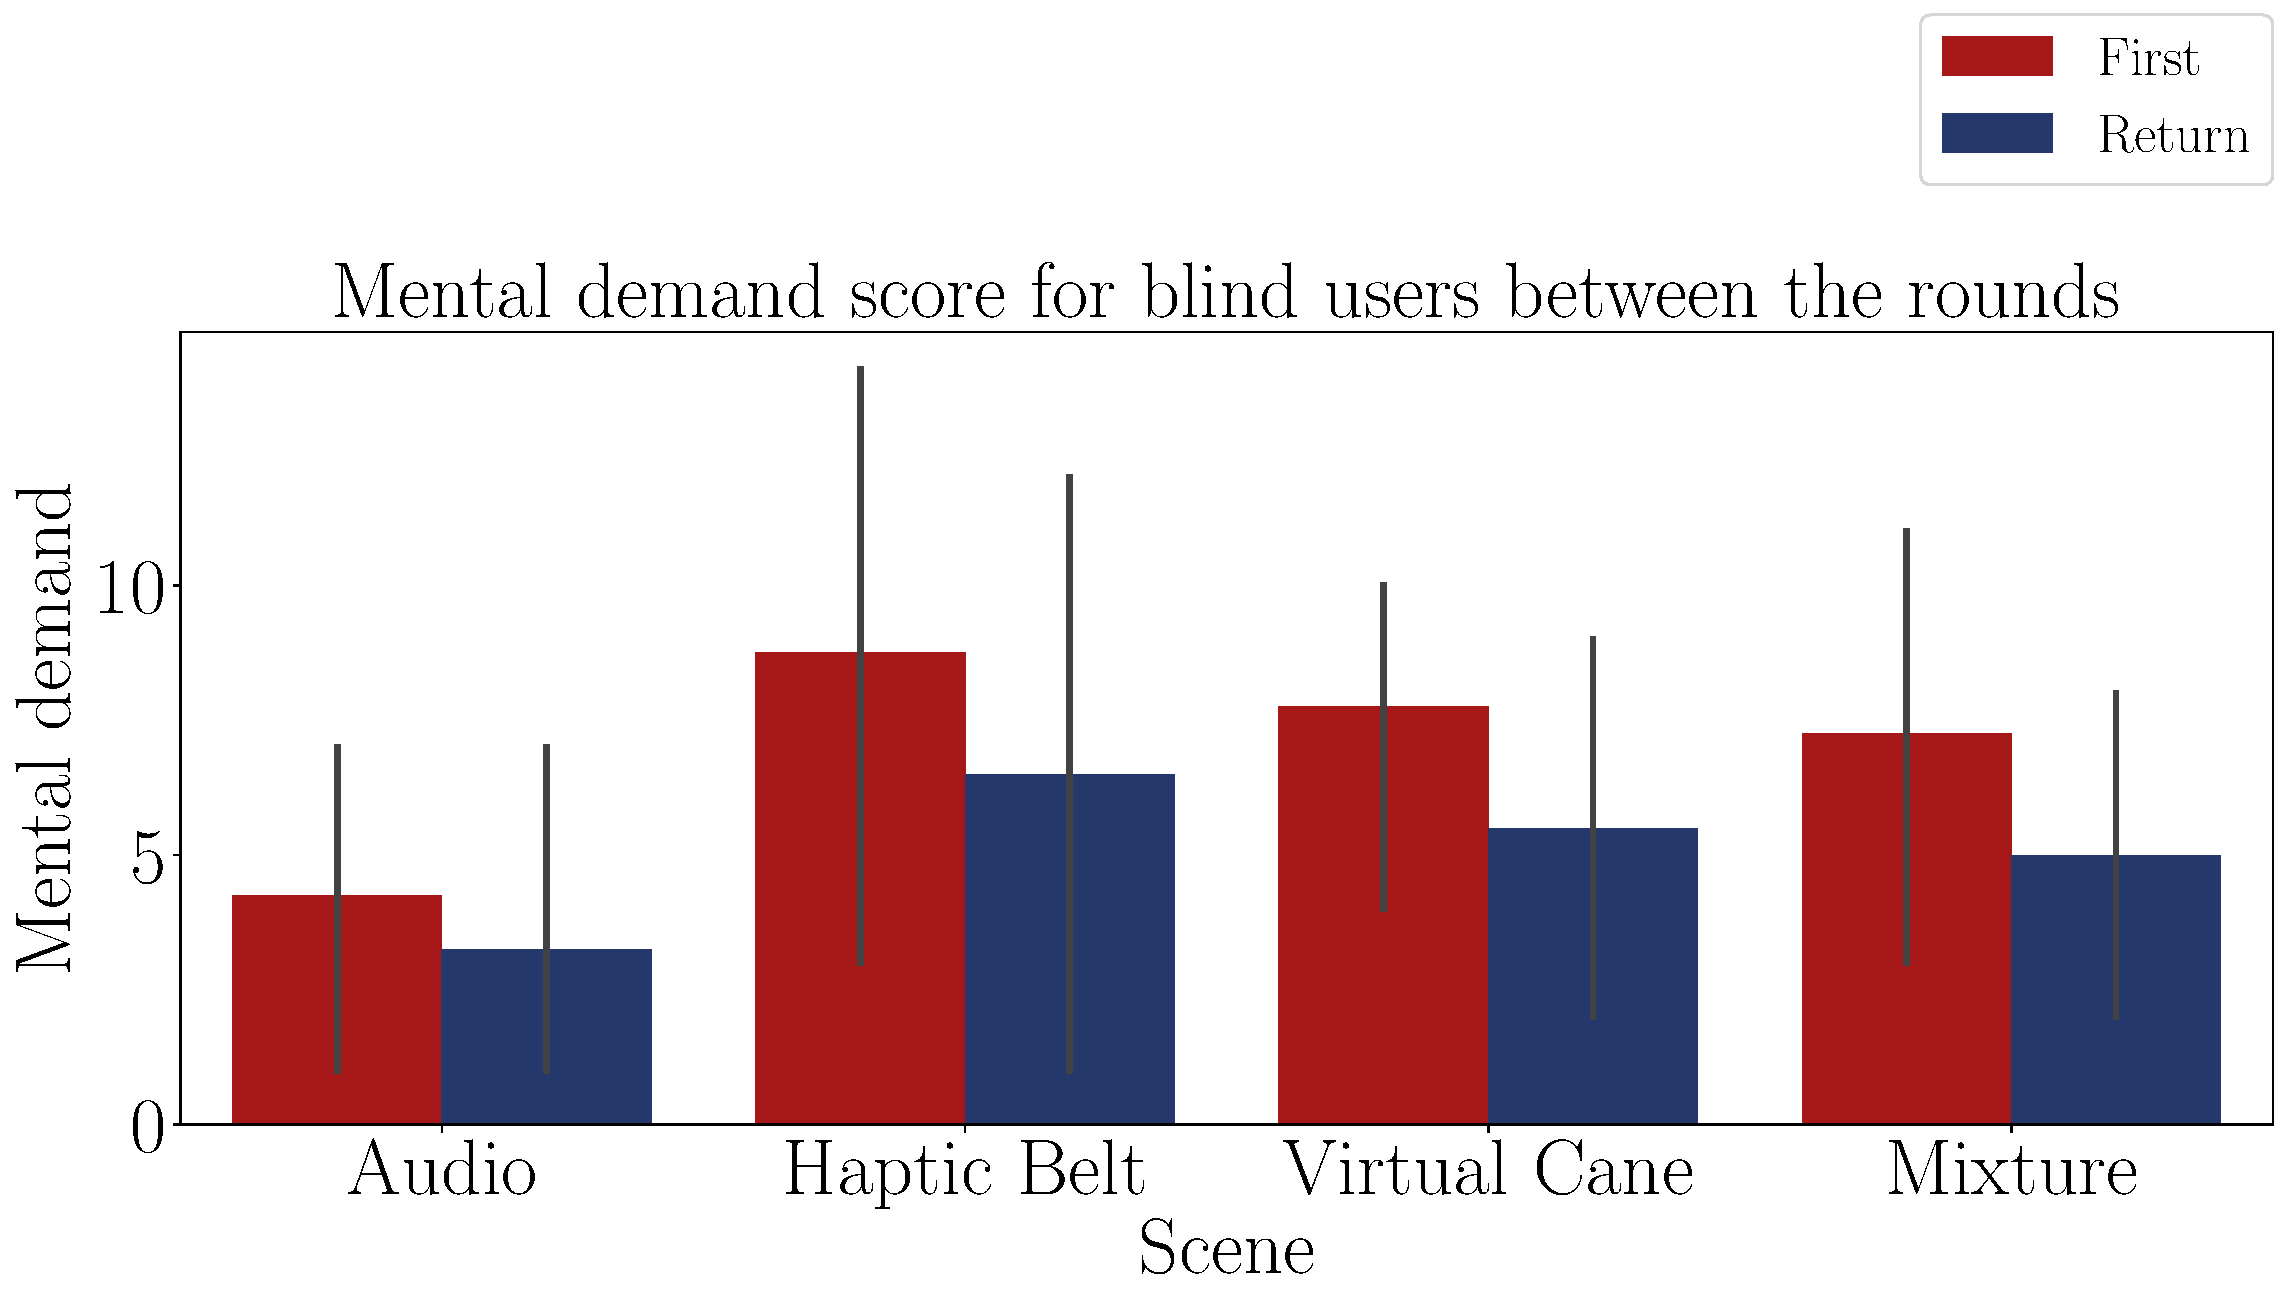
\includegraphics[width = \textwidth]{Resultados/Nasa/Figuras/pdf/barplot_md_avg_4_scene_blind.pdf}
        \subcaption{Blind participants}
        \label{fig:barplot_md_avg_4_scene_blind}
    \end{minipage}
    \begin{minipage}{\textwidth}
        \centering
        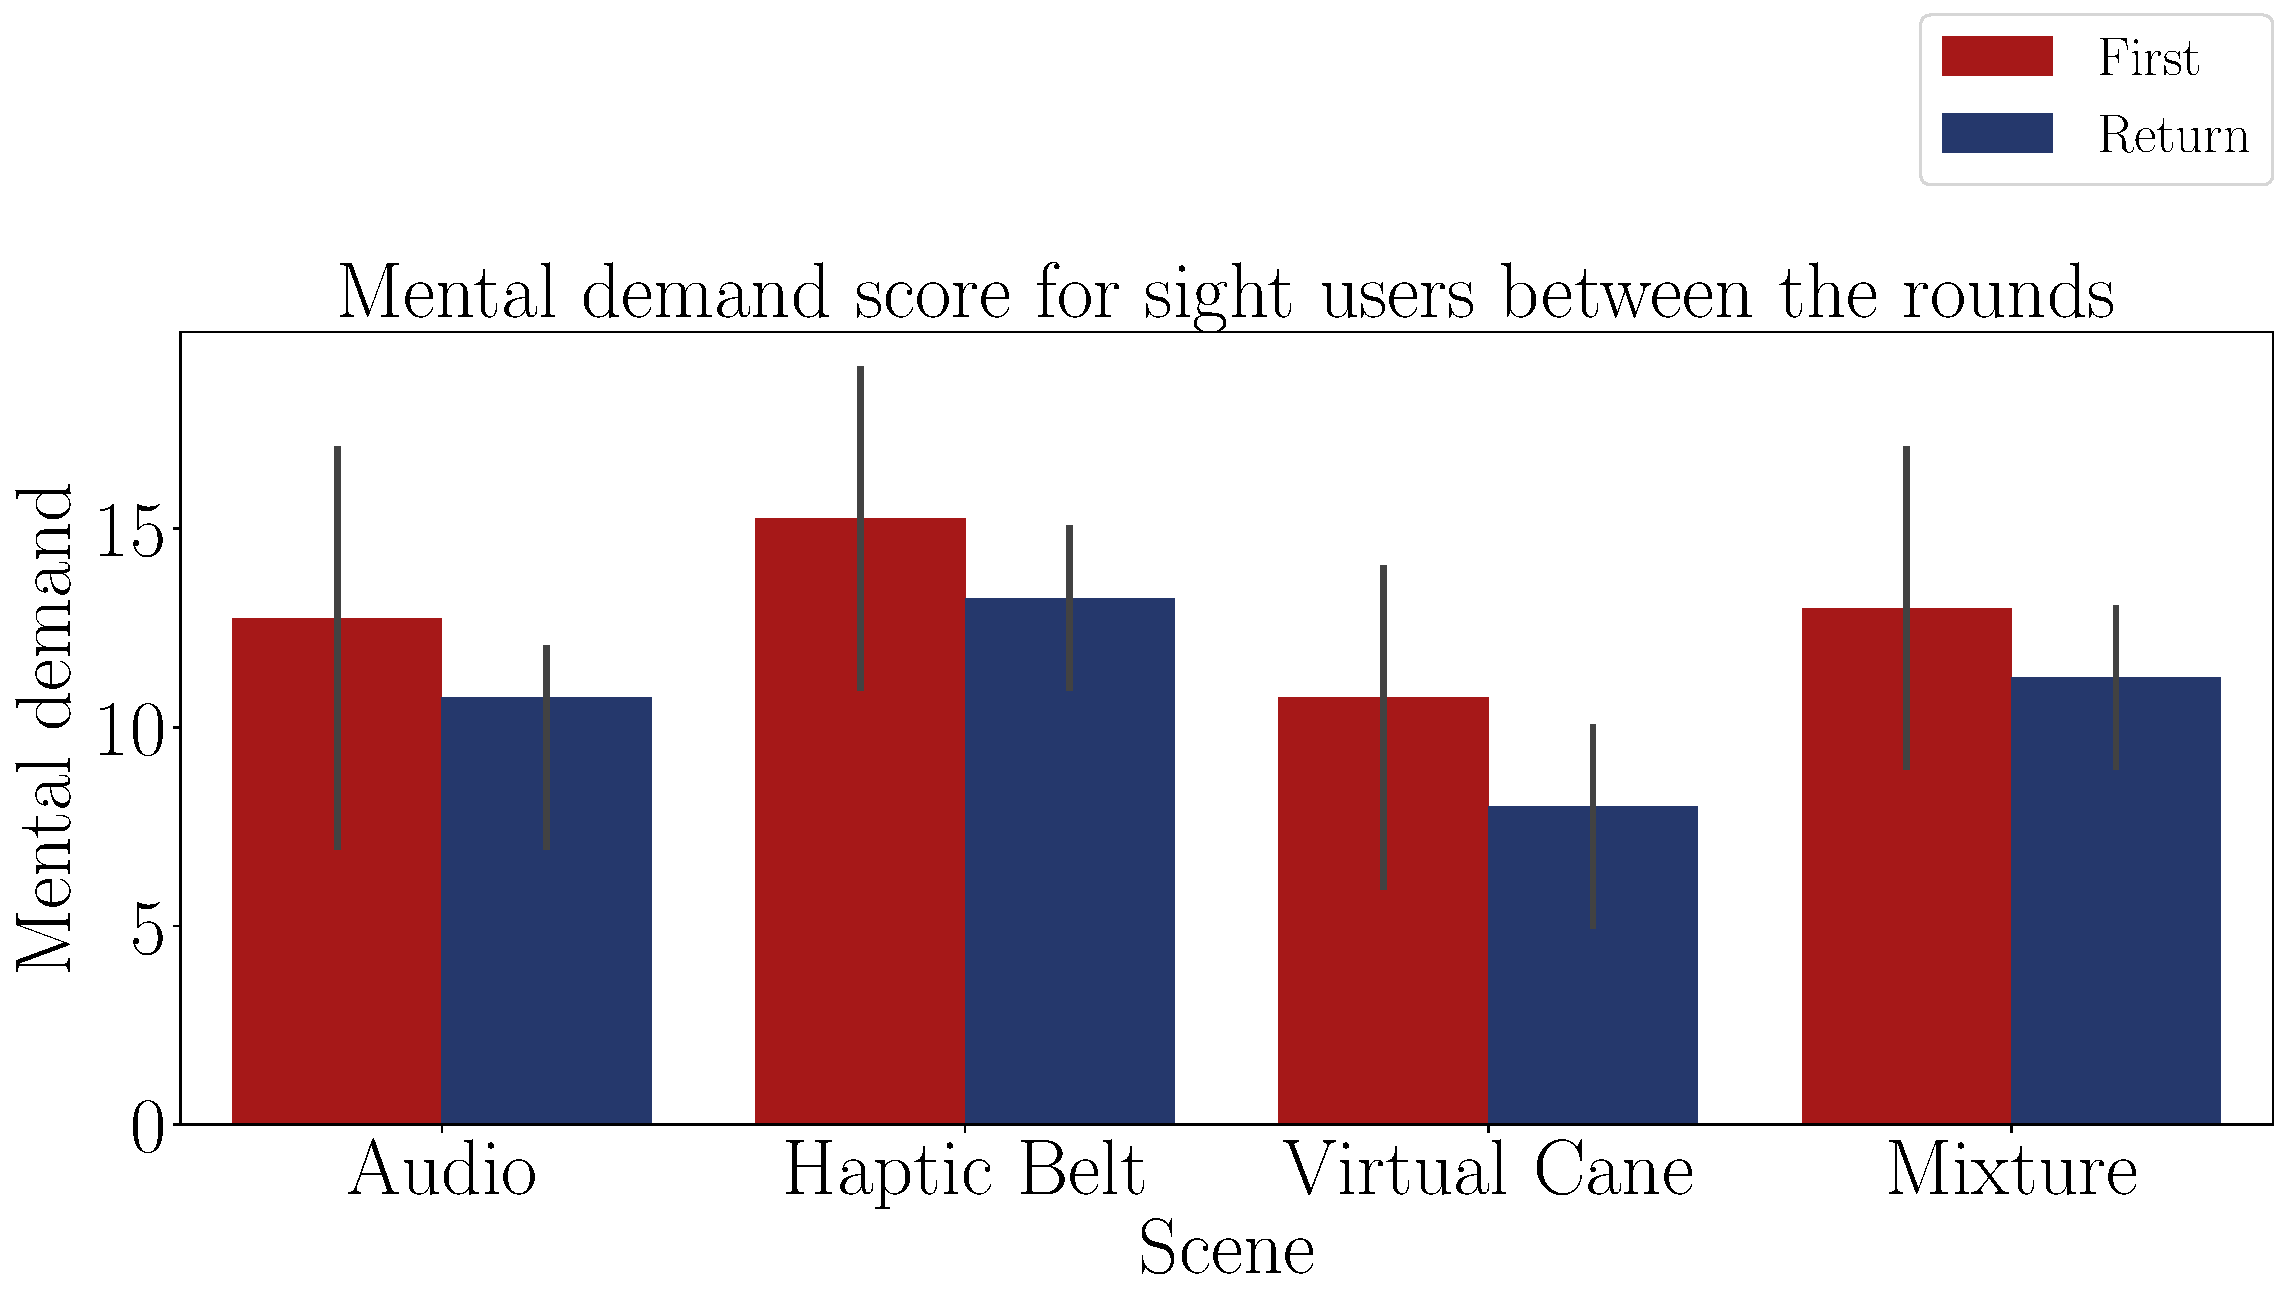
\includegraphics[width = \textwidth]{Resultados/Nasa/Figuras/pdf/barplot_md_avg_4_scene_sight.pdf}
        \subcaption{Sight participants}
        \label{fig:barplot_md_avg_4_scene_sight}
    \end{minipage}
    \caption{Barplot of the average mental demand on each method and round.}
    \label{fig:barplot_md_avg_4_scene_blind_sight}
\end{figure}

Figures \ref{fig:boxplot_noBase_md_4_scene} and \ref{fig:boxplot_noBase_md_4_rounds} presents the box plot for both groups, organized by method and round. It is clear that the mental demand is systematically higher for sighted people, which is something expected. But while blind participants considered the ‘audio’ method less demanding, sighted participants gave preference to the virtual cane. For both groups, we observe a decrease in the mental demand.

\begin{figure}[!htb]
    \centering
    \begin{minipage}{0.45\textwidth}
        \centering
        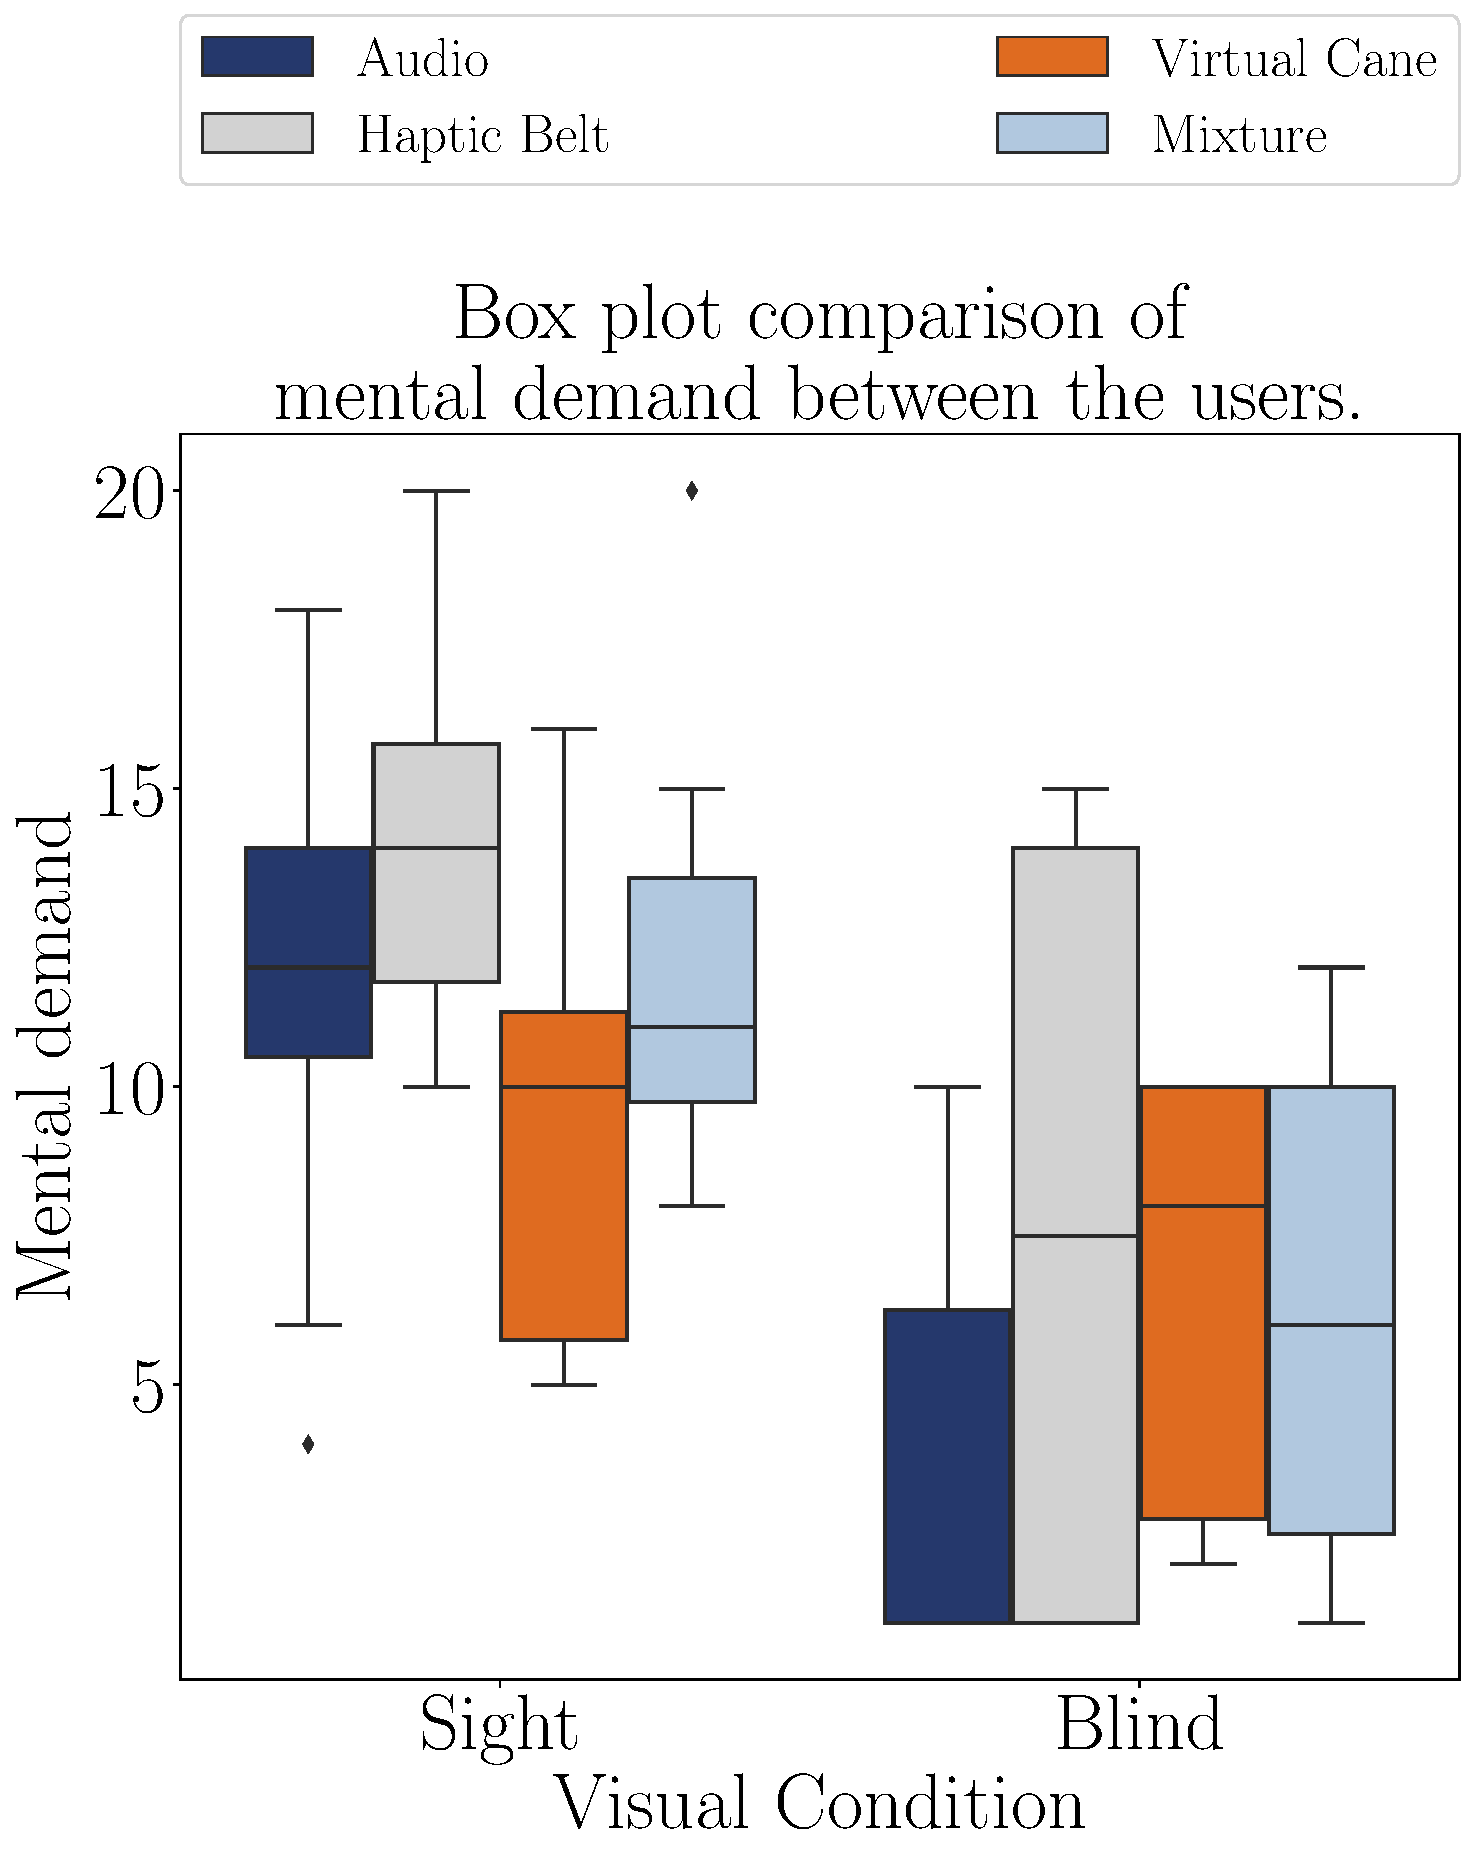
\includegraphics[width = \textwidth]{Resultados/Nasa/Figuras/pdf/boxplot_noBase_md_4_scene.pdf}
        \caption{Boxplot of the mental demand of the participants grouped by method.}
        \label{fig:boxplot_noBase_md_4_scene}
    \end{minipage}
    \begin{minipage}{0.075\textwidth}
        \hfill
    \end{minipage}
    \begin{minipage}{0.45\textwidth}
        \centering
        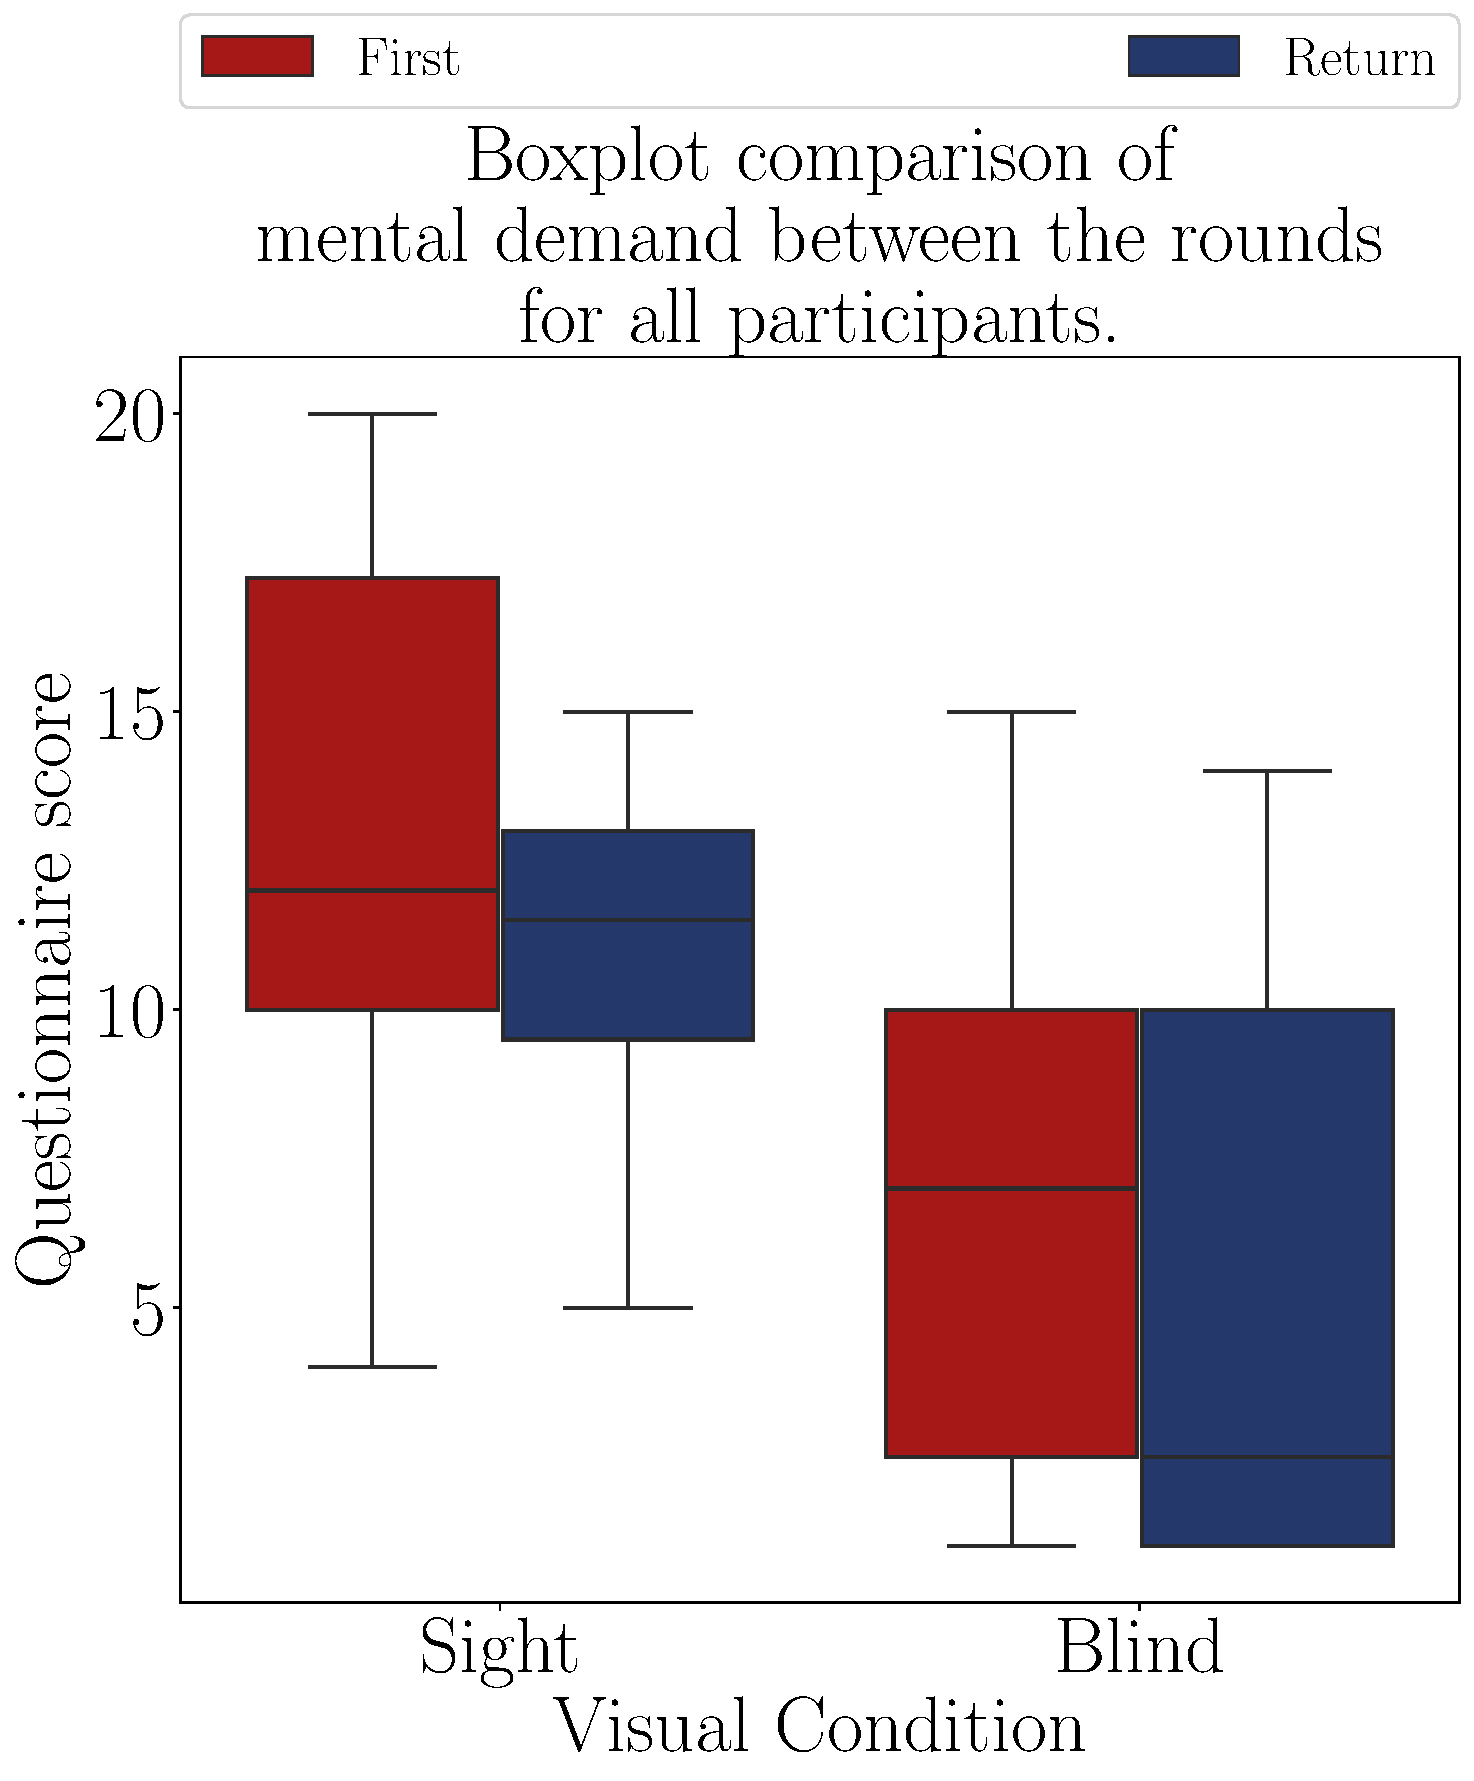
\includegraphics[width = \textwidth]{Resultados/Nasa/Figuras/pdf/boxplot_noBase_md_4_rounds.pdf}
        \caption{Boxplot of the mental demand of the participants grouped by round.}
        \label{fig:boxplot_noBase_md_4_rounds}
    \end{minipage}
\end{figure}

Figures \ref{fig:qqplot_md_avg_two_way_sight} and \ref{fig:residplot_md_avg_two_way_sight} show the QQ plot and residual distribution for the sighted data, confirming that the data is normally distributed and participants have similar variance. Table \ref{tab:blocanova_md_avg_two_way_blind_sight} brings the results of ANOVA. Different from the blind participants, in the case of sighted ones, the p-value for ‘method’ is below the threshold of 0.05, confirming it as a significant variable for the mental demand. In the case of ‘round’, data from both sighted and blind participants resulted in the same p-value of 0.075, which is close to the traditional threshold of 0.05, but slightly higher. 

\begin{table}[!htb]
    \caption{Anova p-value for the mental demand average on each method'}
    \label{tab:blocanova_md_avg_two_way_blind_sight}
\begin{minipage}{0.45\textwidth}
    \subcaption{Blind participants}
    
\centering
\begin{tabular}{ll}
\toprule
          Source & P-Value \\
\midrule
    \    Methods &   0.170 \\
     \    Rounds &   0.075 \\
\    Interaction &   0.993 \\
\bottomrule
\end{tabular}

\end{minipage}
\begin{minipage}{0.45\textwidth}
    \subcaption{Sight participants}
    
\centering
\begin{tabular}{ll}
\toprule
          Source & P-Value \\
\midrule
    \    Methods & 0.049** \\
     \    Rounds &   0.075 \\
\    Interaction &   0.990 \\
\bottomrule
\end{tabular}
    
\end{minipage}
\end{table}

\begin{figure}[!htb]
    \centering
    %\vspace{-15.0cm}
    \begin{minipage}{0.45\textwidth}
        \centering
        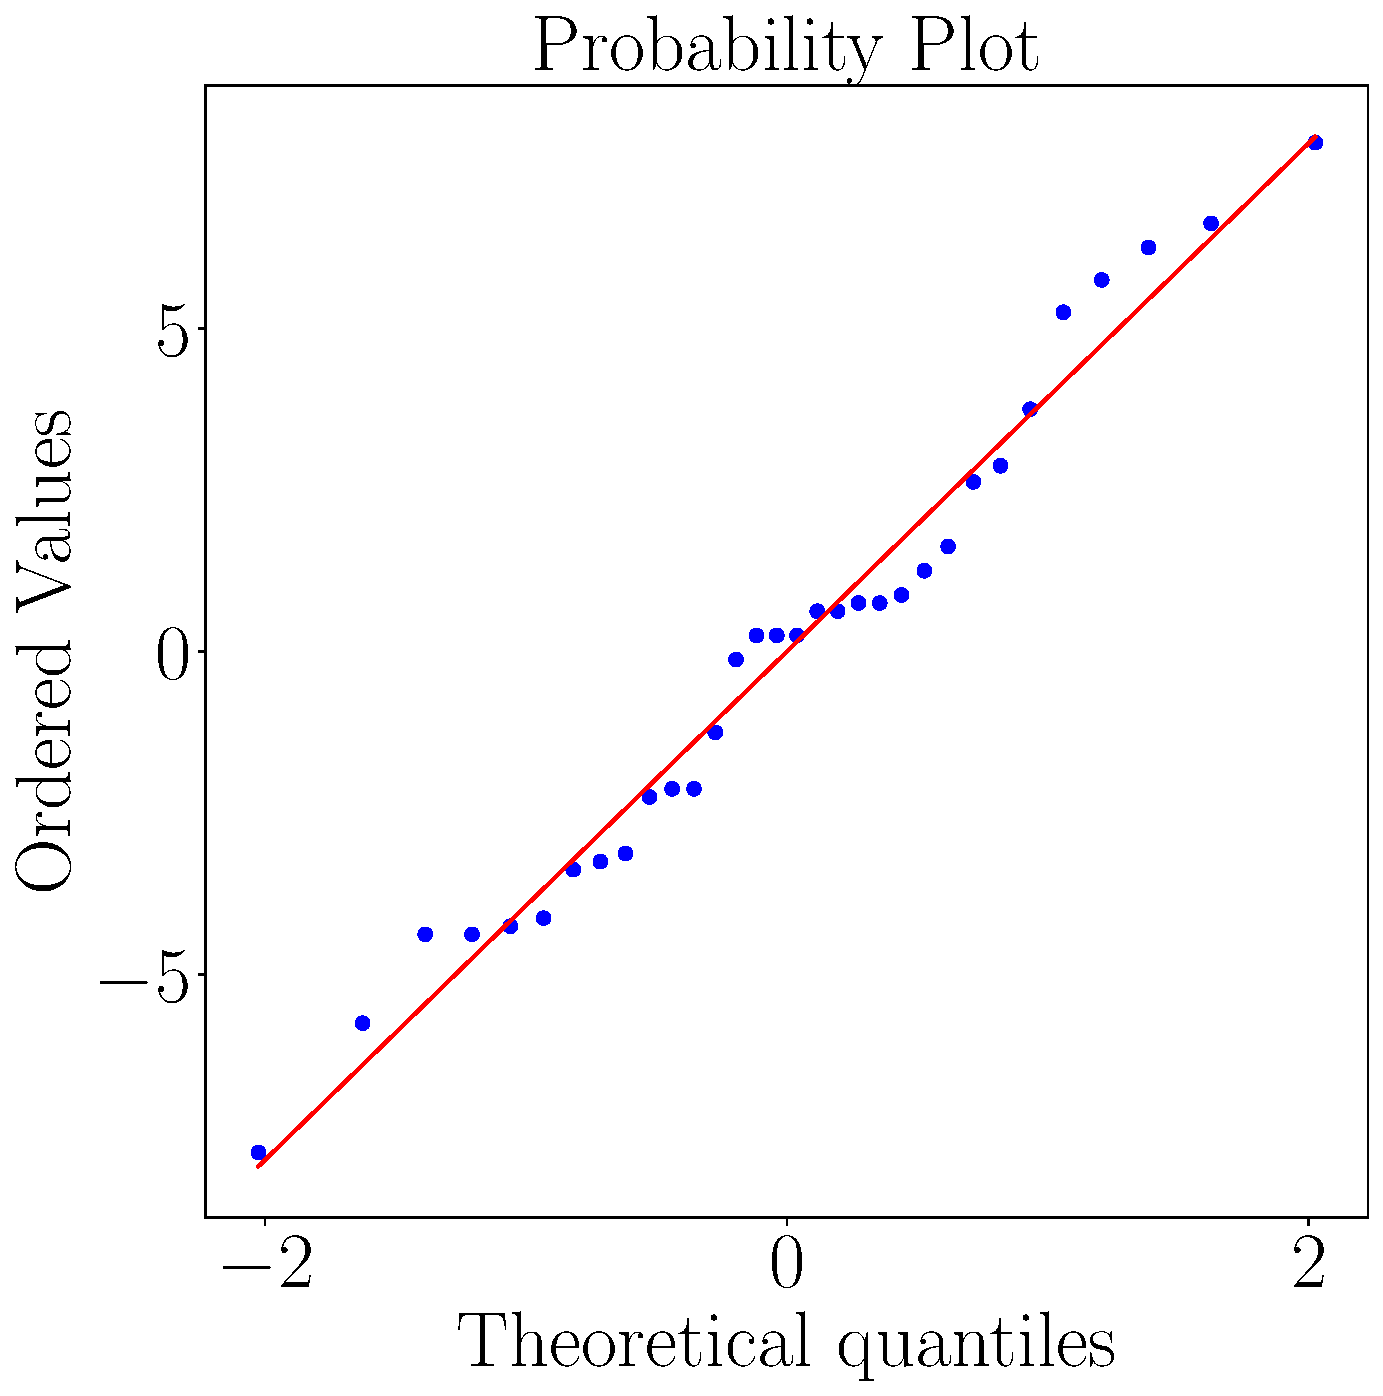
\includegraphics[width = \textwidth]{Resultados/Nasa/Figuras/pdf/qqplot_md_avg_two_way_sight.pdf}
        \caption{QQ plot of the mental demand of the sight participants on each method.}
        \label{fig:qqplot_md_avg_two_way_sight}
    \end{minipage}
    \begin{minipage}{0.075\textwidth}
        \hfill
    \end{minipage}
    \begin{minipage}{0.45\textwidth}
        \centering
        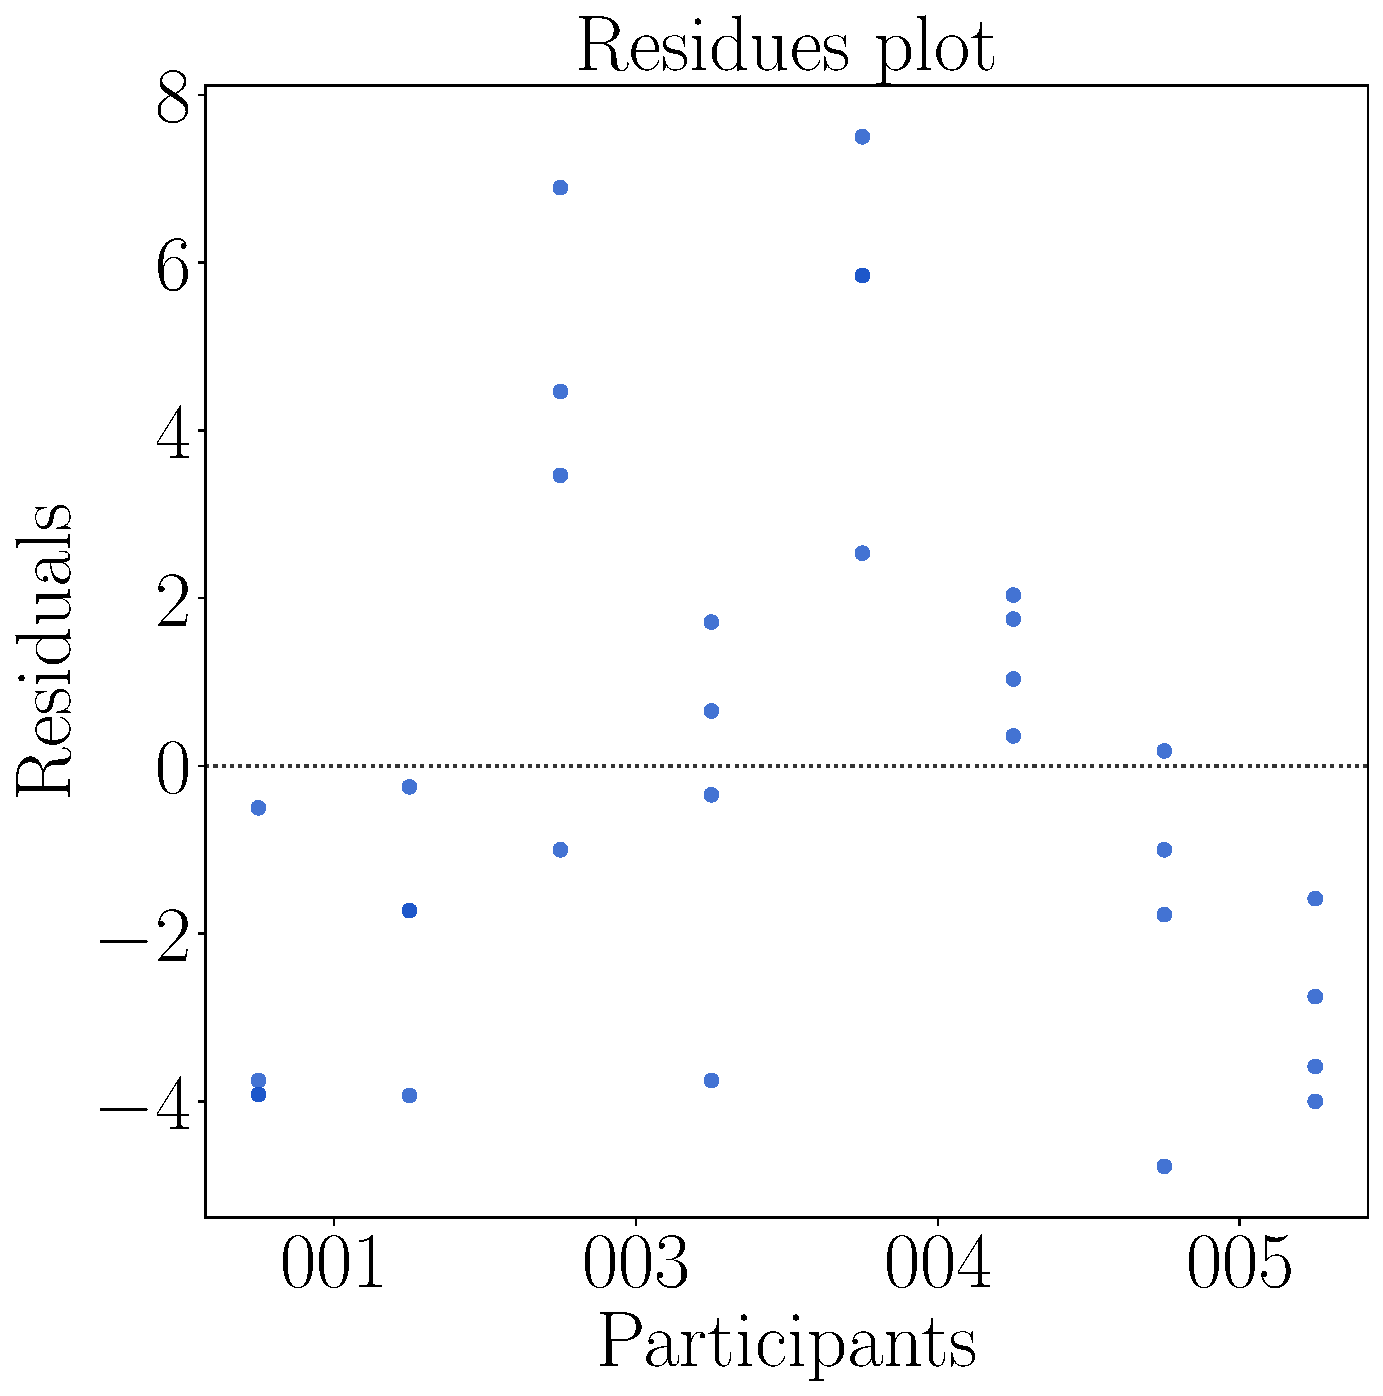
\includegraphics[width = \textwidth]{Resultados/Nasa/Figuras/pdf/residplot_md_avg_two_way_sight.pdf}
        \caption{Residual plot of the mental demand score the sighted participants on each method.}
        \label{fig:residplot_md_avg_two_way_sight}
    \end{minipage}
\end{figure}

\FloatBarrier

%%%%%%%%%%%%%%%%%%%%%%%%%%%%%%%%%%%%%%%%%%%%%%%%%%%%%%%%%%%%%%%%%%%%%%%%%%%%
%%%%%%%%%%%%%%%%%%%%%%%%%%%%%%%%%%%%%%%%%%%%%%%%%%%%%%%%%%%%%%%%%%%%%%%%%%%%
%%%%%%%%%%%%%%%%%%%%%%%%%%%%%%%%%%%%%%%%%%%%%%%%%%%%%%%%%%%%%%%%%%%%%%%%%%%%
%%%%%%%%%%%%%%%%%%%%%%%%%%%%%%%%%%%%%%%%%%%%%%%%%%%%%%%%%%%%%%%%%%%%%%%%%%%%


\paragraph{Analysis of the NASA-TLX score}\mbox{}\\

Table \ref{tab:nasa_table_noBase} brings the NASA-TLX global score of all participants, while the corresponding barplot is presented in Figure \ref{fig:barplot_nasa_avg_4_scene}.


\begin{table}[!htb]
\centering
\caption{NASA-TLX score felled by the participants.}
\label{tab:nasa_table_noBase}
\begin{tabular}{lllrrrrr}
\toprule
    &       &        &  Audio & \begin{tabular}[c]{@{}l@{}}Haptic\\ Belt\end{tabular} & \begin{tabular}[c]{@{}l@{}}Virtual\\ Cane\end{tabular} & Mixture \\
Participant & \begin{tabular}[c]{@{}l@{}}Visual\\ Condition\end{tabular} & Round &        &                                                       &                                                        &         \\
\midrule
001 & Sight & First & 10.167 &                                                 9.833 &                                                  7.000 &   9.000 \\
    &       & Return & 11.000 &                                                10.833 &                                                  6.167 &   9.333 \\
001C & Blind & First &  4.000 &                                                 8.833 &                                                  5.167 &   6.333 \\
    &       & Return &  4.000 &                                                 6.667 &                                                  4.500 &   6.167 \\
002C & Blind & First &  4.833 &                                                 4.833 &                                                  9.000 &   7.000 \\
    &       & Return &  4.833 &                                                 4.833 &                                                  7.000 &   5.167 \\
003 & Sight & First &  9.833 &                                                10.167 &                                                  9.500 &   6.500 \\
    &       & Return &  6.667 &                                                 9.667 &                                                  7.833 &   4.833 \\
003C & Blind & First &  4.000 &                                                 5.333 &                                                  6.667 &   3.500 \\
    &       & Return &  3.833 &                                                 3.667 &                                                  3.500 &   3.500 \\
004 & Sight & First & 14.833 &                                                13.667 &                                                 11.500 &  15.833 \\
    &       & Return & 11.833 &                                                11.833 &                                                 10.833 &  12.167 \\
004C & Blind & First & 10.000 &                                                12.667 &                                                  9.667 &  11.000 \\
    &       & Return &  9.167 &                                                11.667 &                                                  9.333 &  10.833 \\
005 & Sight & First &  7.667 &                                                 9.000 &                                                  8.000 &   9.667 \\
    &       & Return &  7.667 &                                                 8.667 &                                                  7.667 &   6.000 \\
\bottomrule
\end{tabular}
\end{table}



From Figure \ref{fig:barplot_nasa_avg_4_scene} it is possible to see that, similar to blind participants, sighted participants also consider that the workload of the return round was lower than that of the first round. However, similar to what happened for the mental demand, sighted participants considered ‘virtual cane’ as the method with the lowest workload, while, for  blind participants, it was the ‘audio’.

\begin{figure}[!htb]
    \centering
    \begin{minipage}{\textwidth}
        \centering
        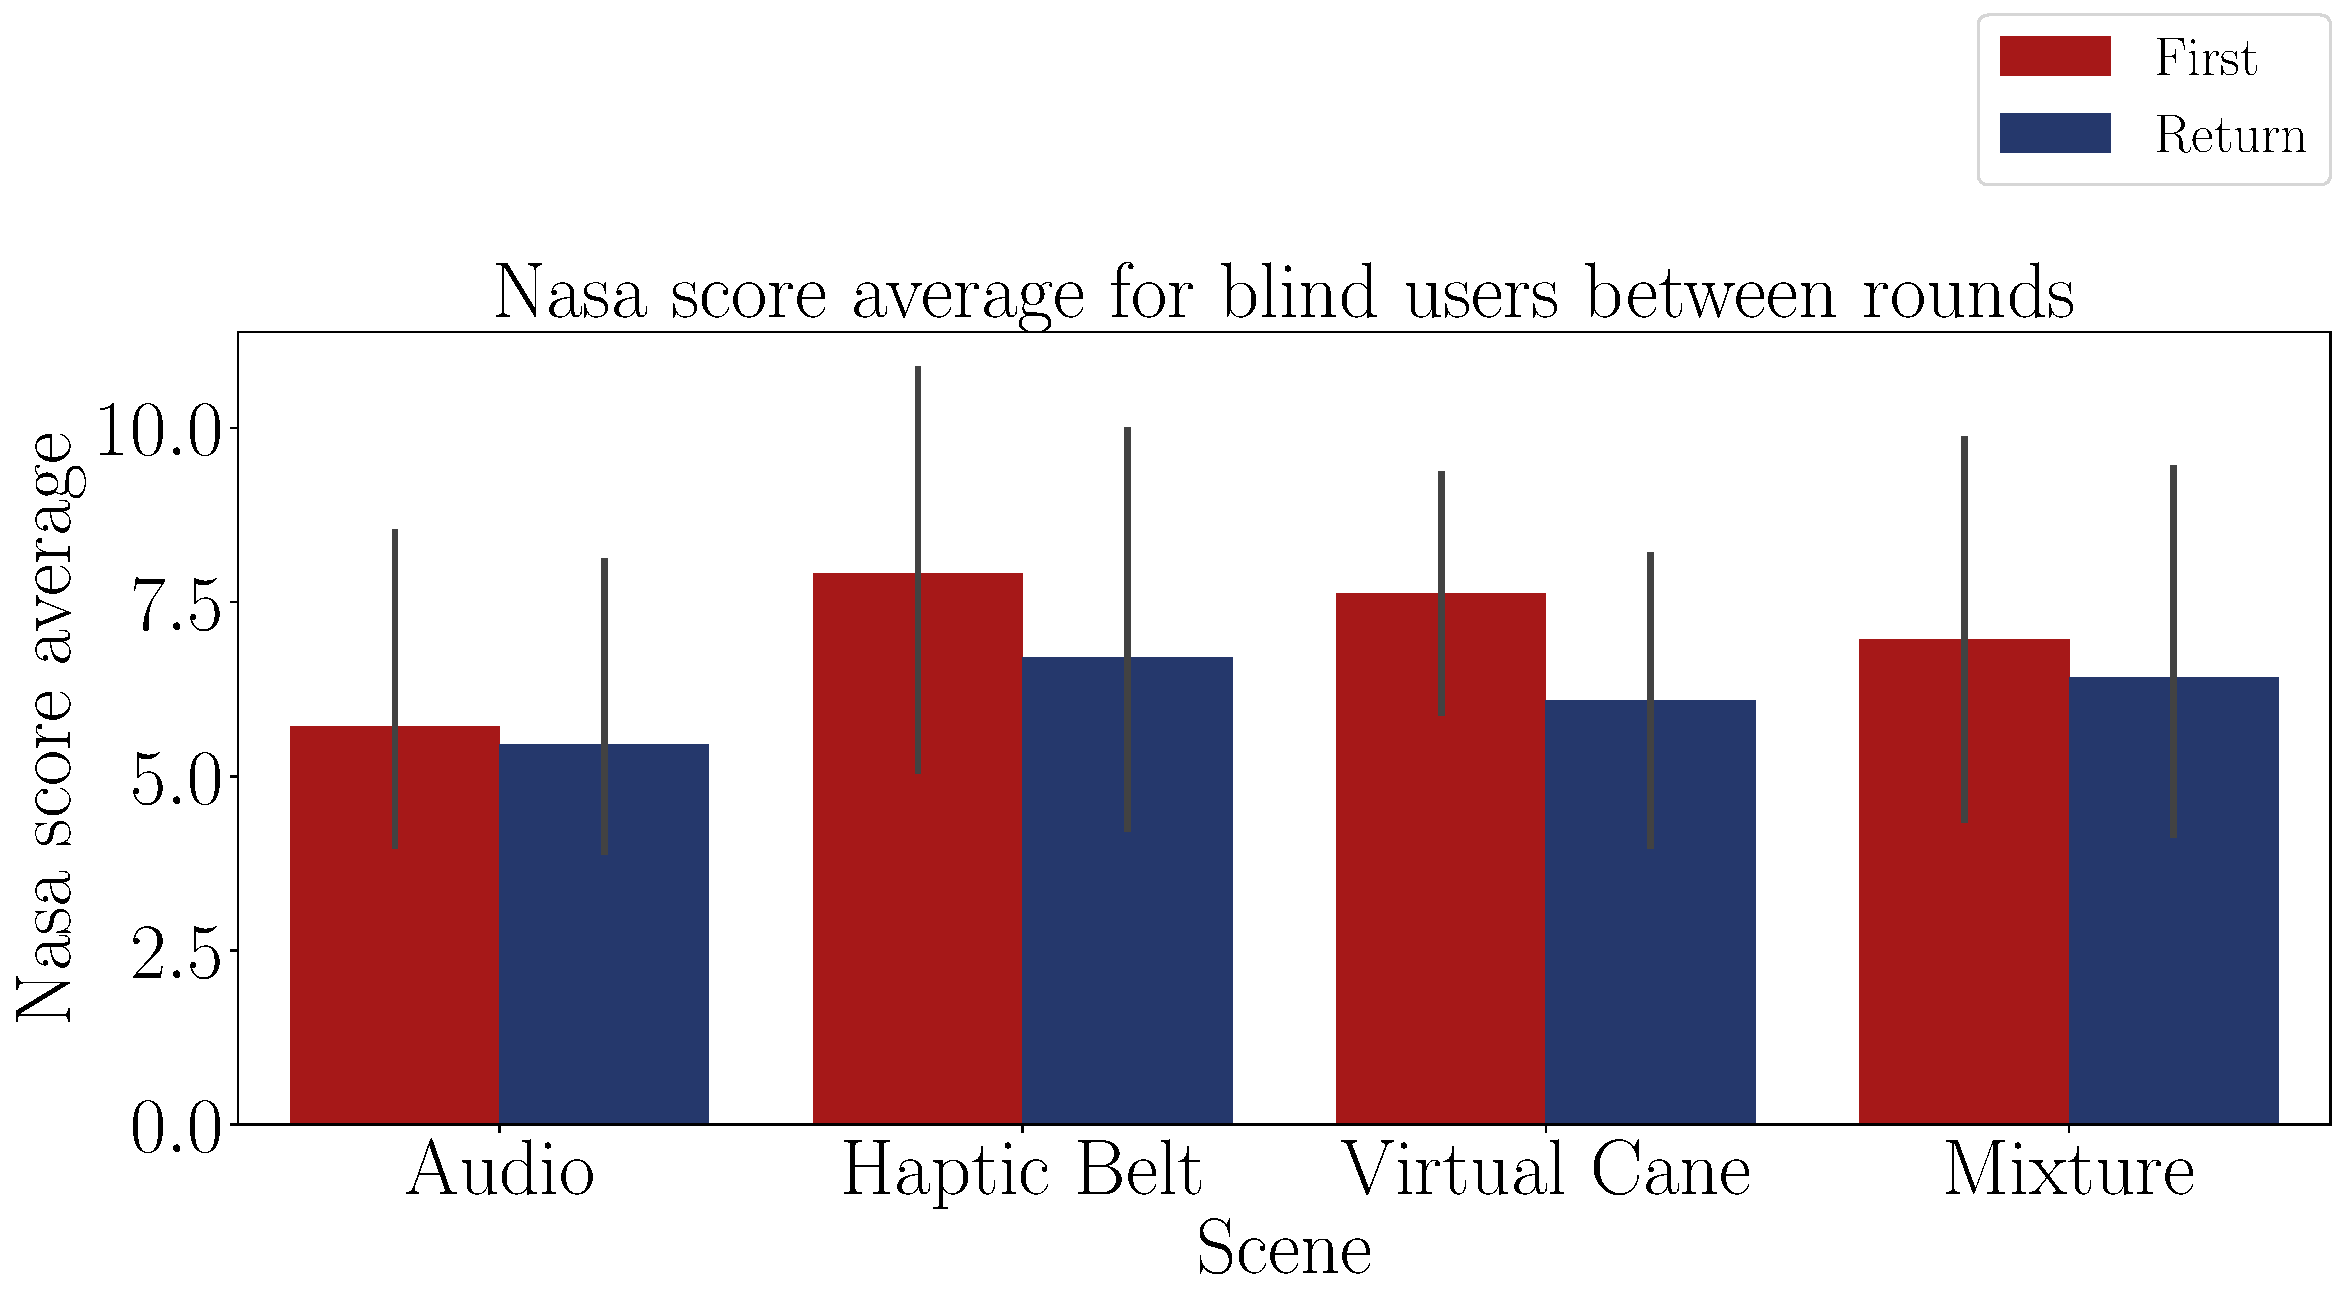
\includegraphics[width = \textwidth]{Resultados/Nasa/Figuras/pdf/barplot_nasa_avg_4_scene_blind.pdf}
        \subcaption{Blind participants.}
        \label{fig:barplot_nasa_avg_4_scene_blind}
    \end{minipage}
    \begin{minipage}{\textwidth}
        \centering
        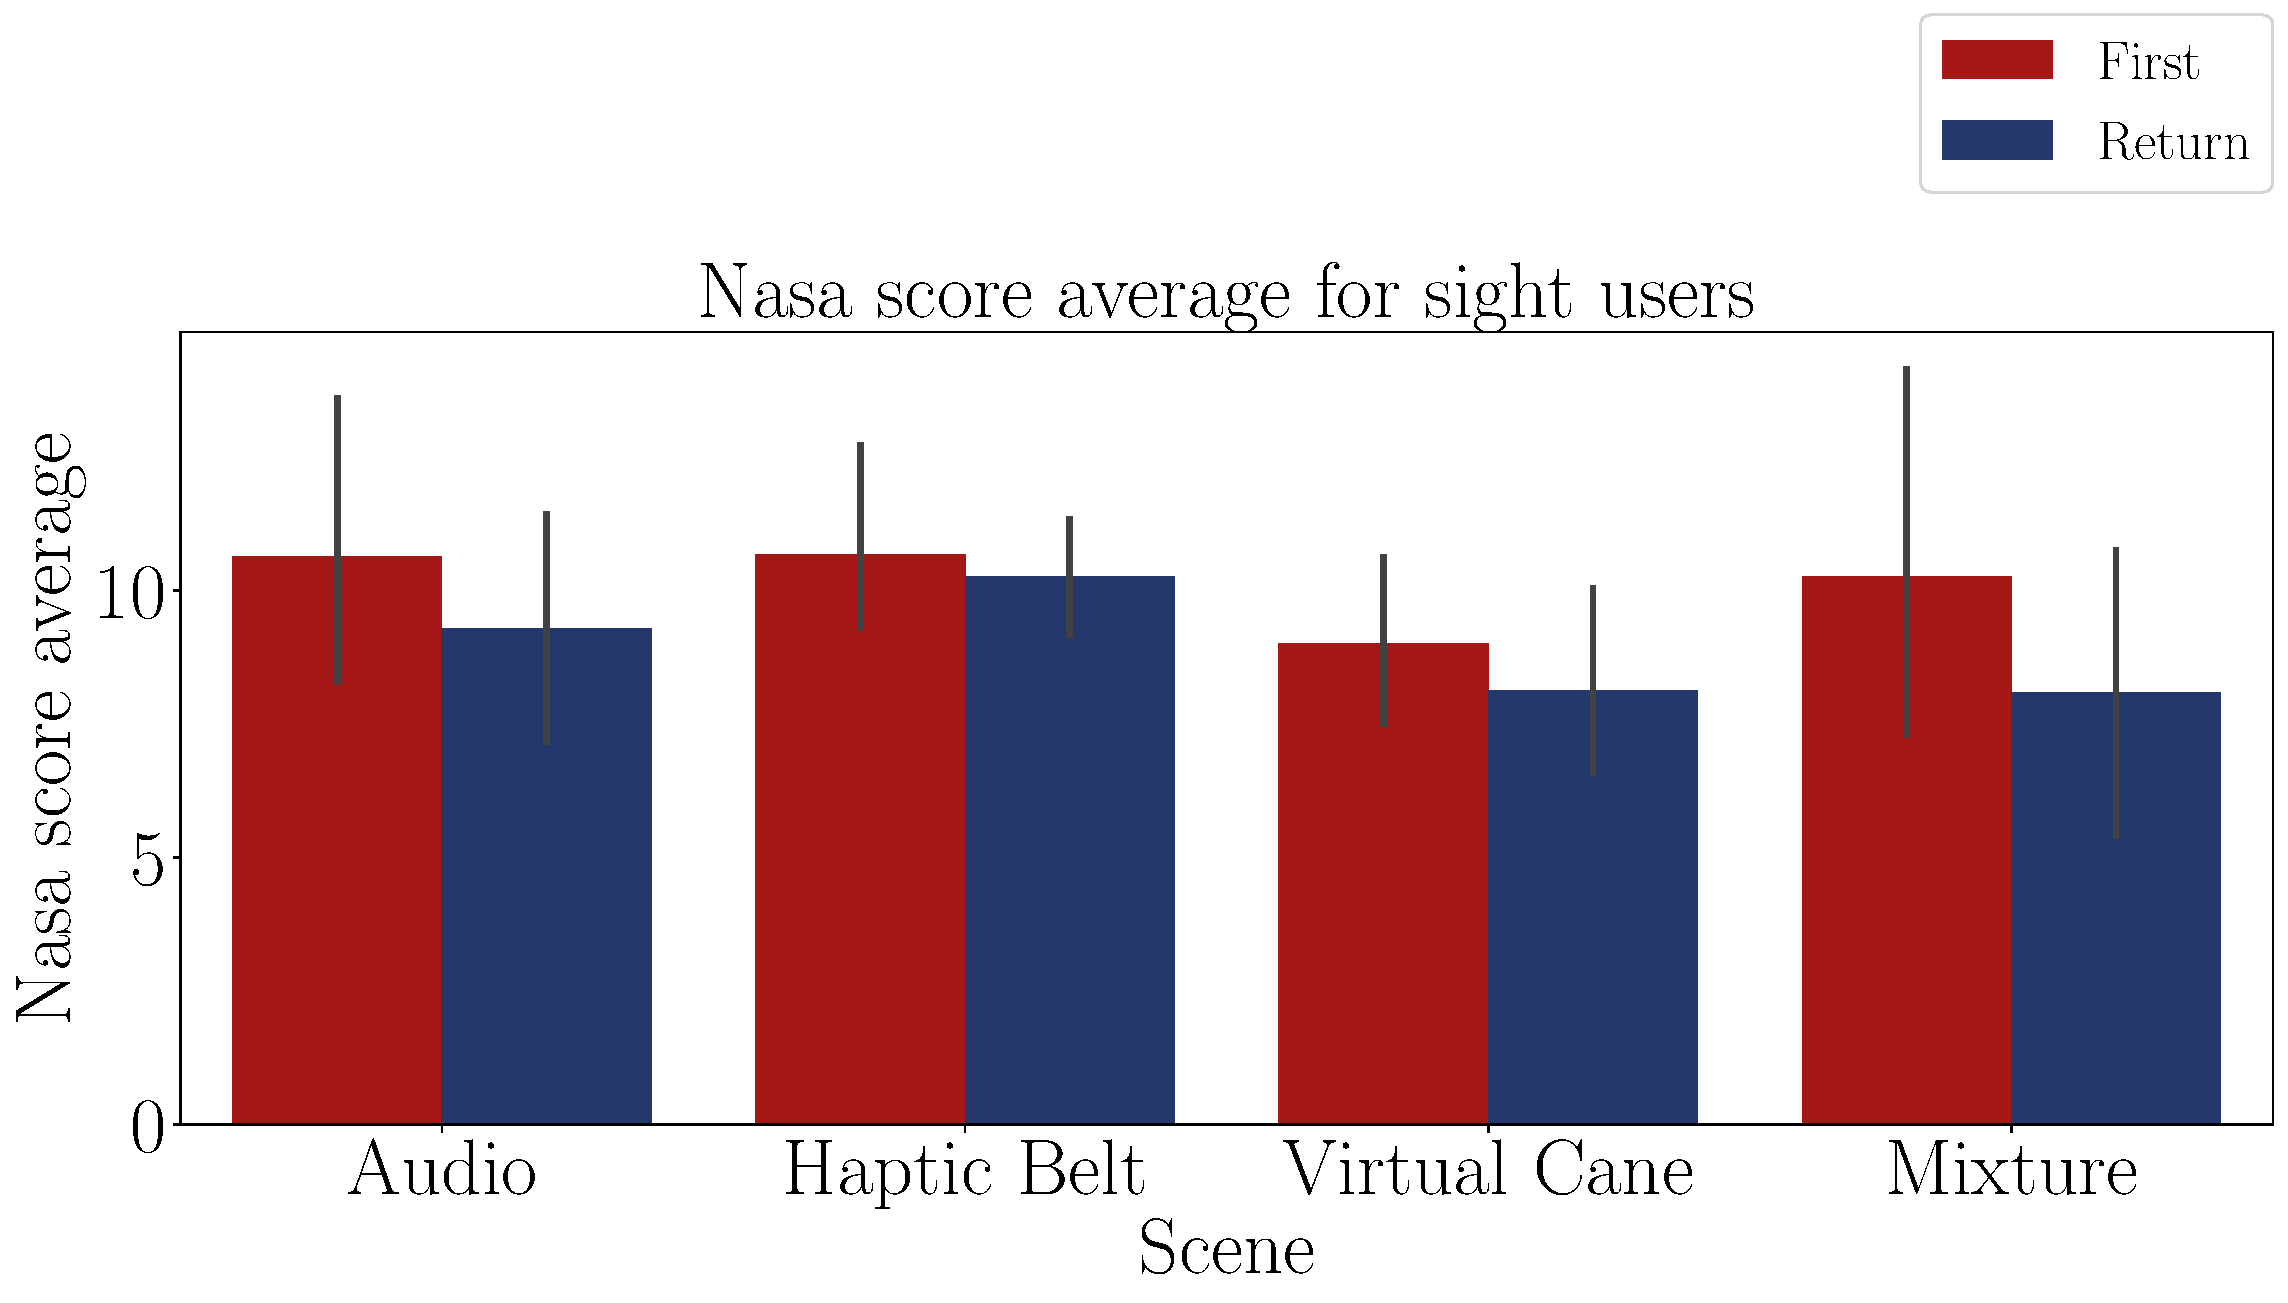
\includegraphics[width = \textwidth]{Resultados/Nasa/Figuras/pdf/barplot_nasa_avg_4_scene_sight.pdf}
        \subcaption{Sight participants.}
        \label{fig:barplot_nasa_avg_4_scene_sight}
    \end{minipage}
    \caption{Barplot of the NASA-TLX score on each method and round.}
    \label{fig:barplot_nasa_avg_4_scene}
\end{figure}

Figures \ref{fig:boxplot_noBase_nasa_4_scene} and \ref{fig:boxplot_noBase_nasa_4_rounds} present the boxplots of NASA-TLX global score. Again, it is possible to see that sighted people usually give higher workload scores than blind ones. The influence of the round is approximately the same. But the order of preference of the methods are different.

\begin{figure}[!htb]
    \centering
    \begin{minipage}{0.45\textwidth}
        \centering
        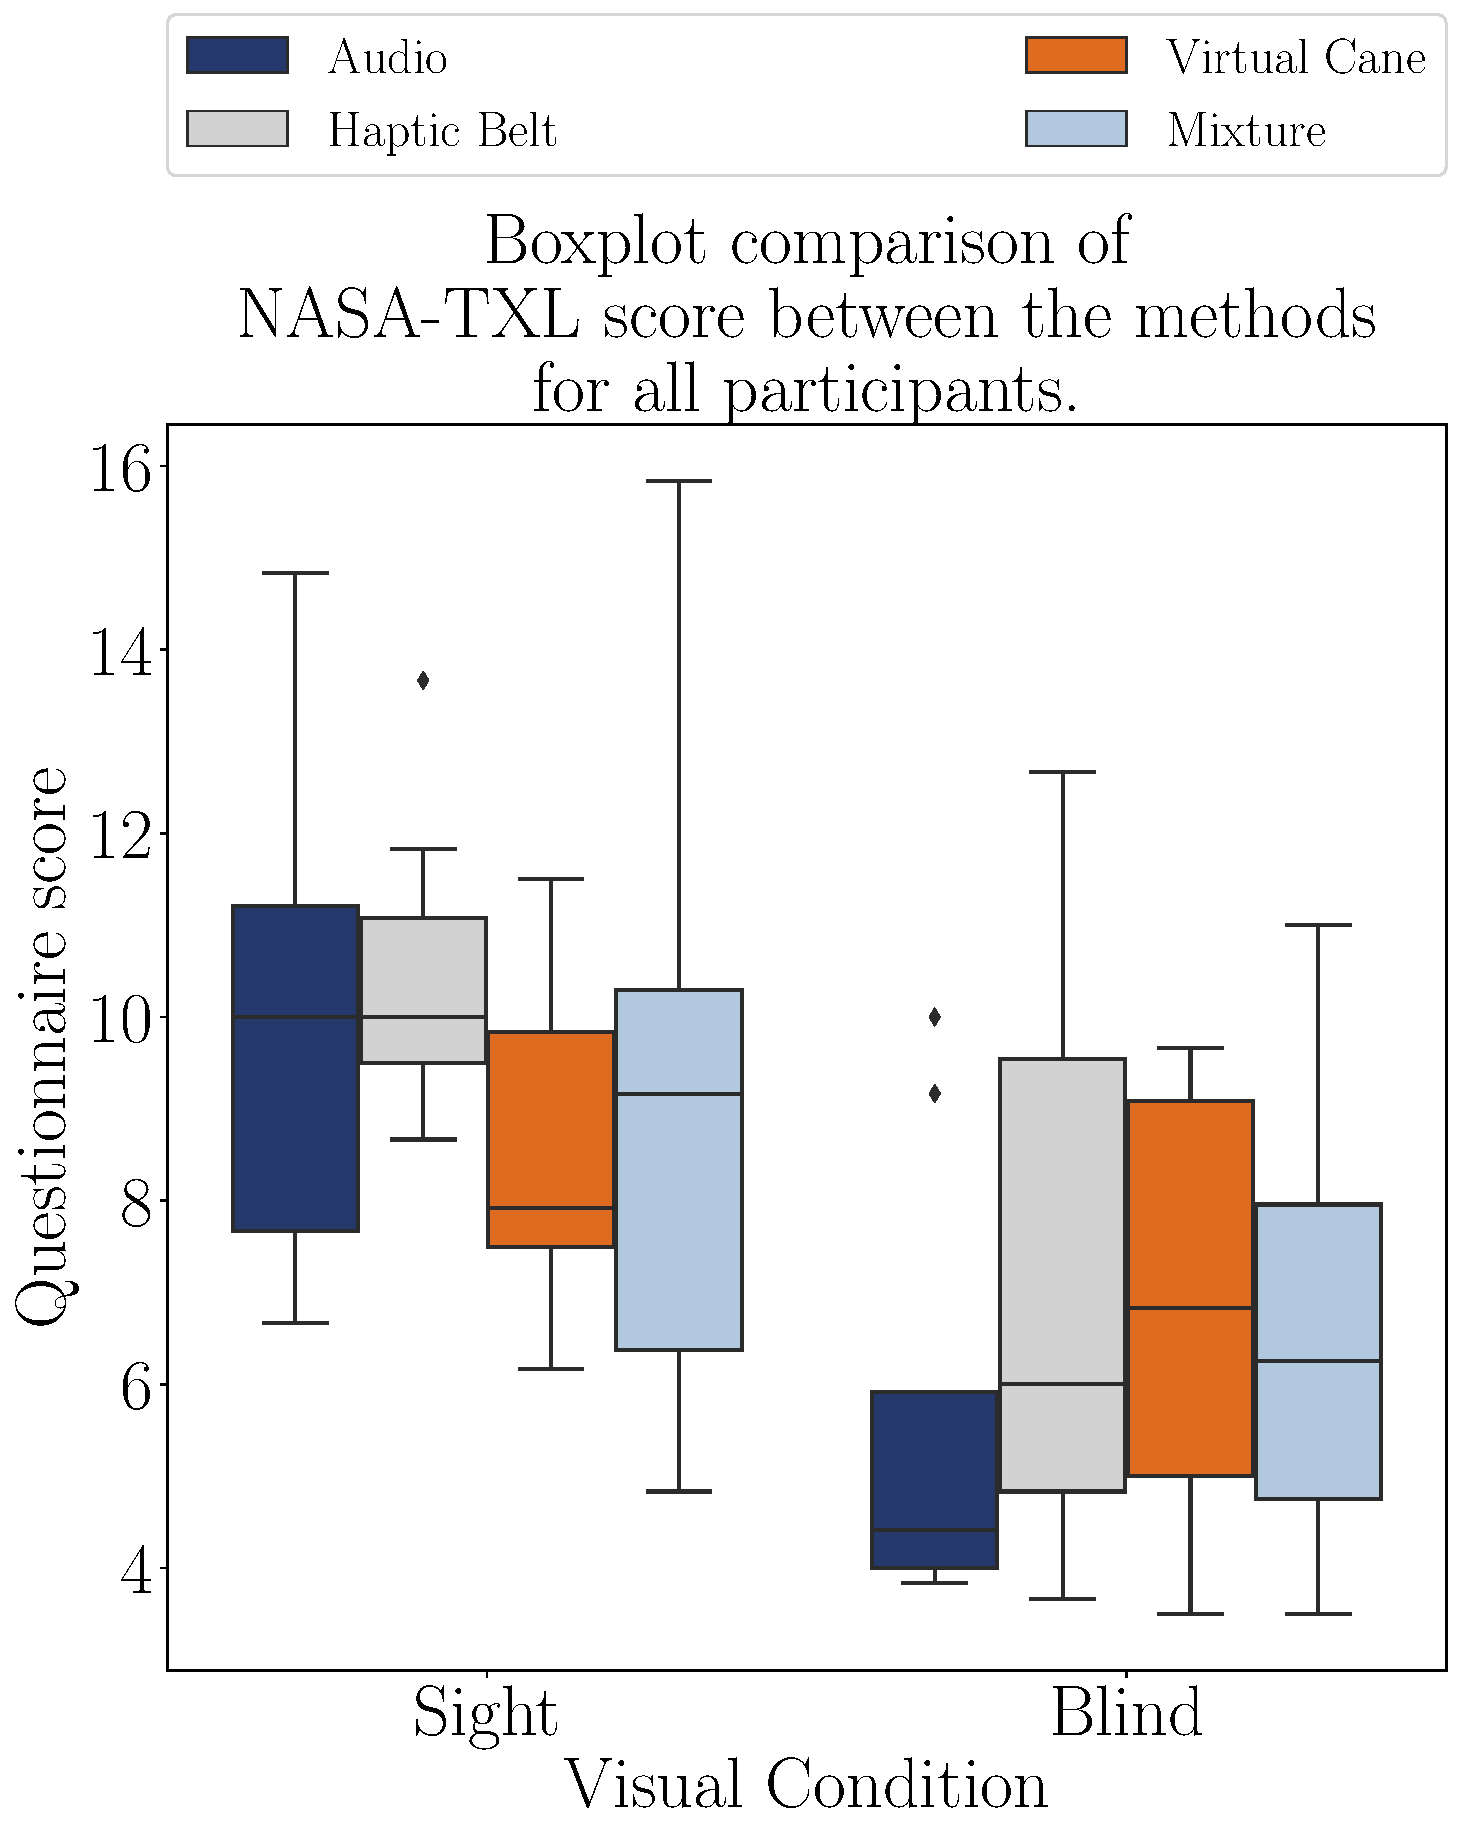
\includegraphics[width = \textwidth]{Resultados/Nasa/Figuras/pdf/boxplot_noBase_nasa_4_scene.pdf}
        \caption{Boxplot of the NASA-TLX score of the participants grouped by method.}
        \label{fig:boxplot_noBase_nasa_4_scene}
    \end{minipage}
    \begin{minipage}{0.075\textwidth}
        \hfill
    \end{minipage}
    \begin{minipage}{0.45\textwidth}
        \centering
        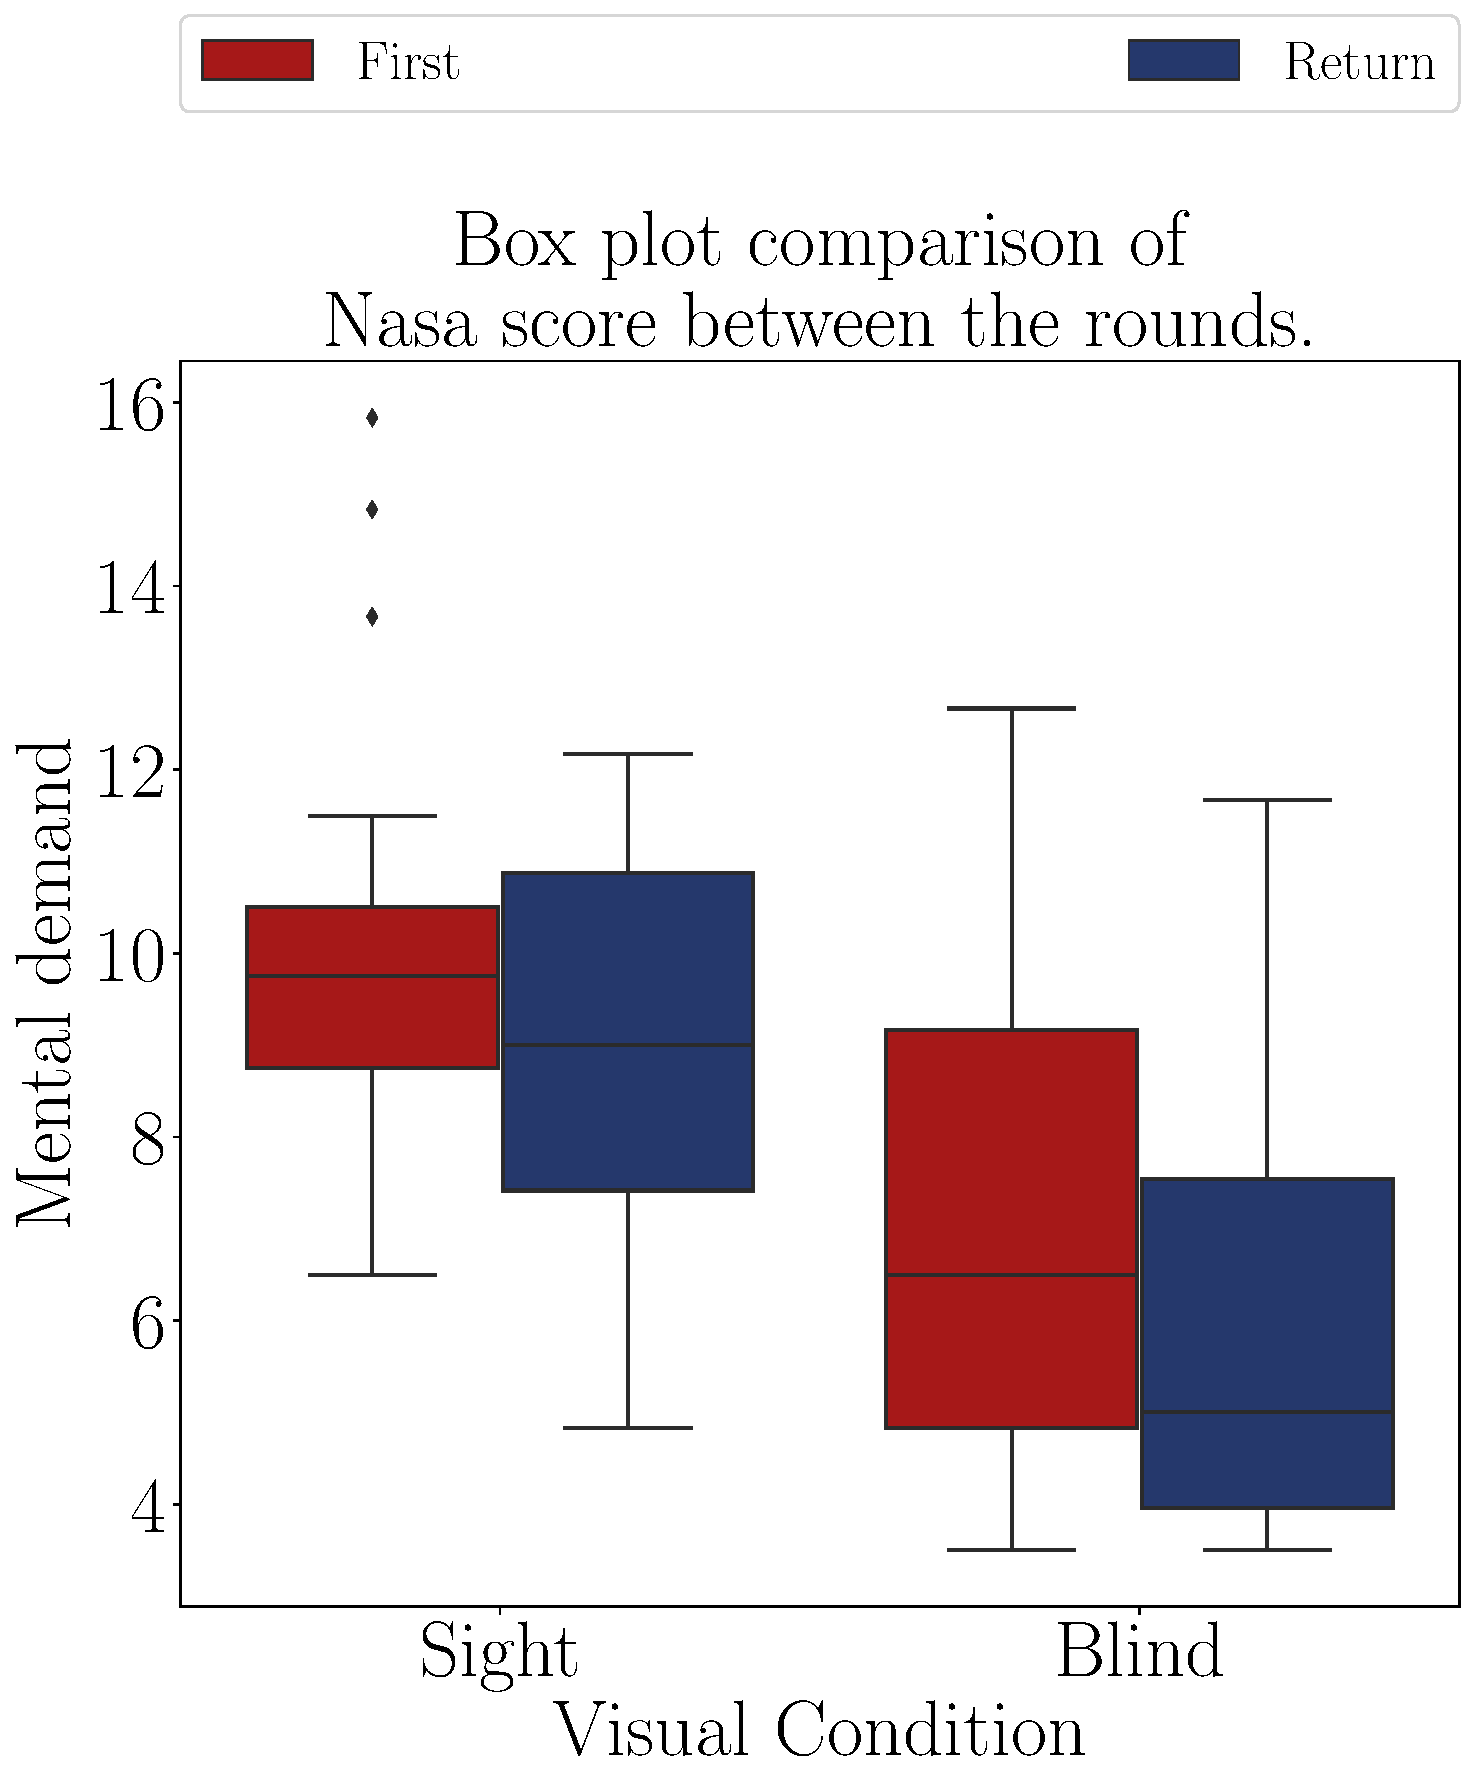
\includegraphics[width = \textwidth]{Resultados/Nasa/Figuras/pdf/boxplot_noBase_nasa_4_rounds.pdf}
        \caption{Boxplot of the NASA-TLX score of the participants grouped by round.}
        \label{fig:boxplot_noBase_nasa_4_rounds}
    \end{minipage}
\end{figure}

Figures \ref{fig:qqplot_nasa_avg_two_way_sight} and \ref{fig:residplot_nasa_avg_two_way_sight} bring the QQ plot and residual distribution of the data from sighted participants, showing that ANOVA can be used. The p-values for both groups are presented in Table \ref{tab:blocanova_nasa_avg_two_way_blind_sight}. It confirms the influence of the round for both sighted and blind people. In the case of the method, the p-value of ‘blind’ is lower than the threshold of 0.5, while that of ‘sighted’ is slightly higher.

\begin{table}[!thb]
    \caption{Anova p-value for the NASA-TLX score on each method}
    \label{tab:blocanova_nasa_avg_two_way_blind_sight}
    \begin{minipage}{0.45\textwidth}
        \subcaption{Blind participants}
        
\centering
\begin{tabular}{ll}
\toprule
          Source & P-Value \\
\midrule
    \    Methods & 0.029** \\
     \    Rounds & 0.022** \\
\    Interaction &   0.814 \\
\bottomrule
\end{tabular}

    \end{minipage}
    \begin{minipage}{0.45\textwidth}
        \subcaption{Sight participants}
        
\centering
\begin{tabular}{ll}
\toprule
          Source & P-Value \\
\midrule
    \    Methods &   0.086 \\
     \    Rounds & 0.034** \\
\    Interaction &   0.688 \\
\bottomrule
\end{tabular}
    
    \end{minipage}
\end{table}


\begin{figure}[!htb]
    \centering
    %\vspace{-15.0cm}
    \begin{minipage}{0.45\textwidth}
        \centering
        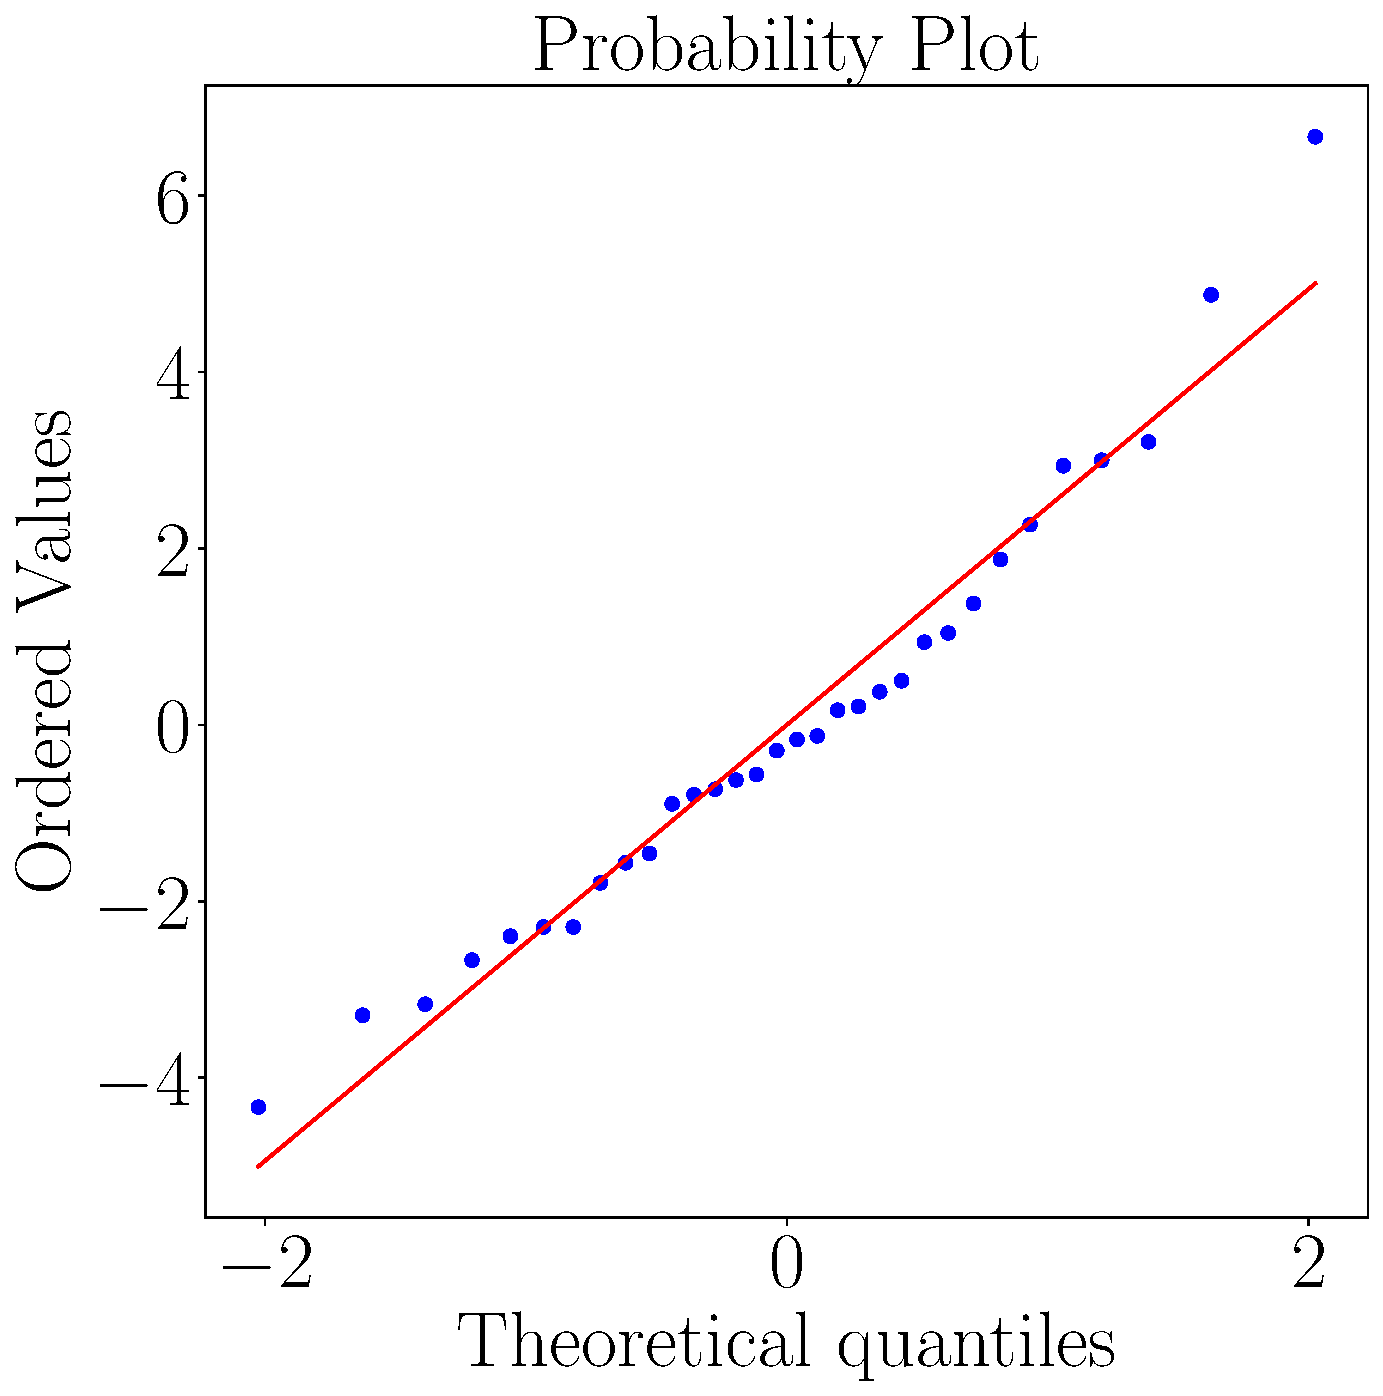
\includegraphics[width = \textwidth]{Resultados/Nasa/Figuras/pdf/qqplot_nasa_avg_two_way_sight.pdf}
        \caption{QQ plot of the NASA-TLX score of the sight participants on each method.}
        \label{fig:qqplot_nasa_avg_two_way_sight}
    \end{minipage}
    \begin{minipage}{0.075\textwidth}
        \hfill
    \end{minipage}
    \begin{minipage}{0.45\textwidth}
        \centering
        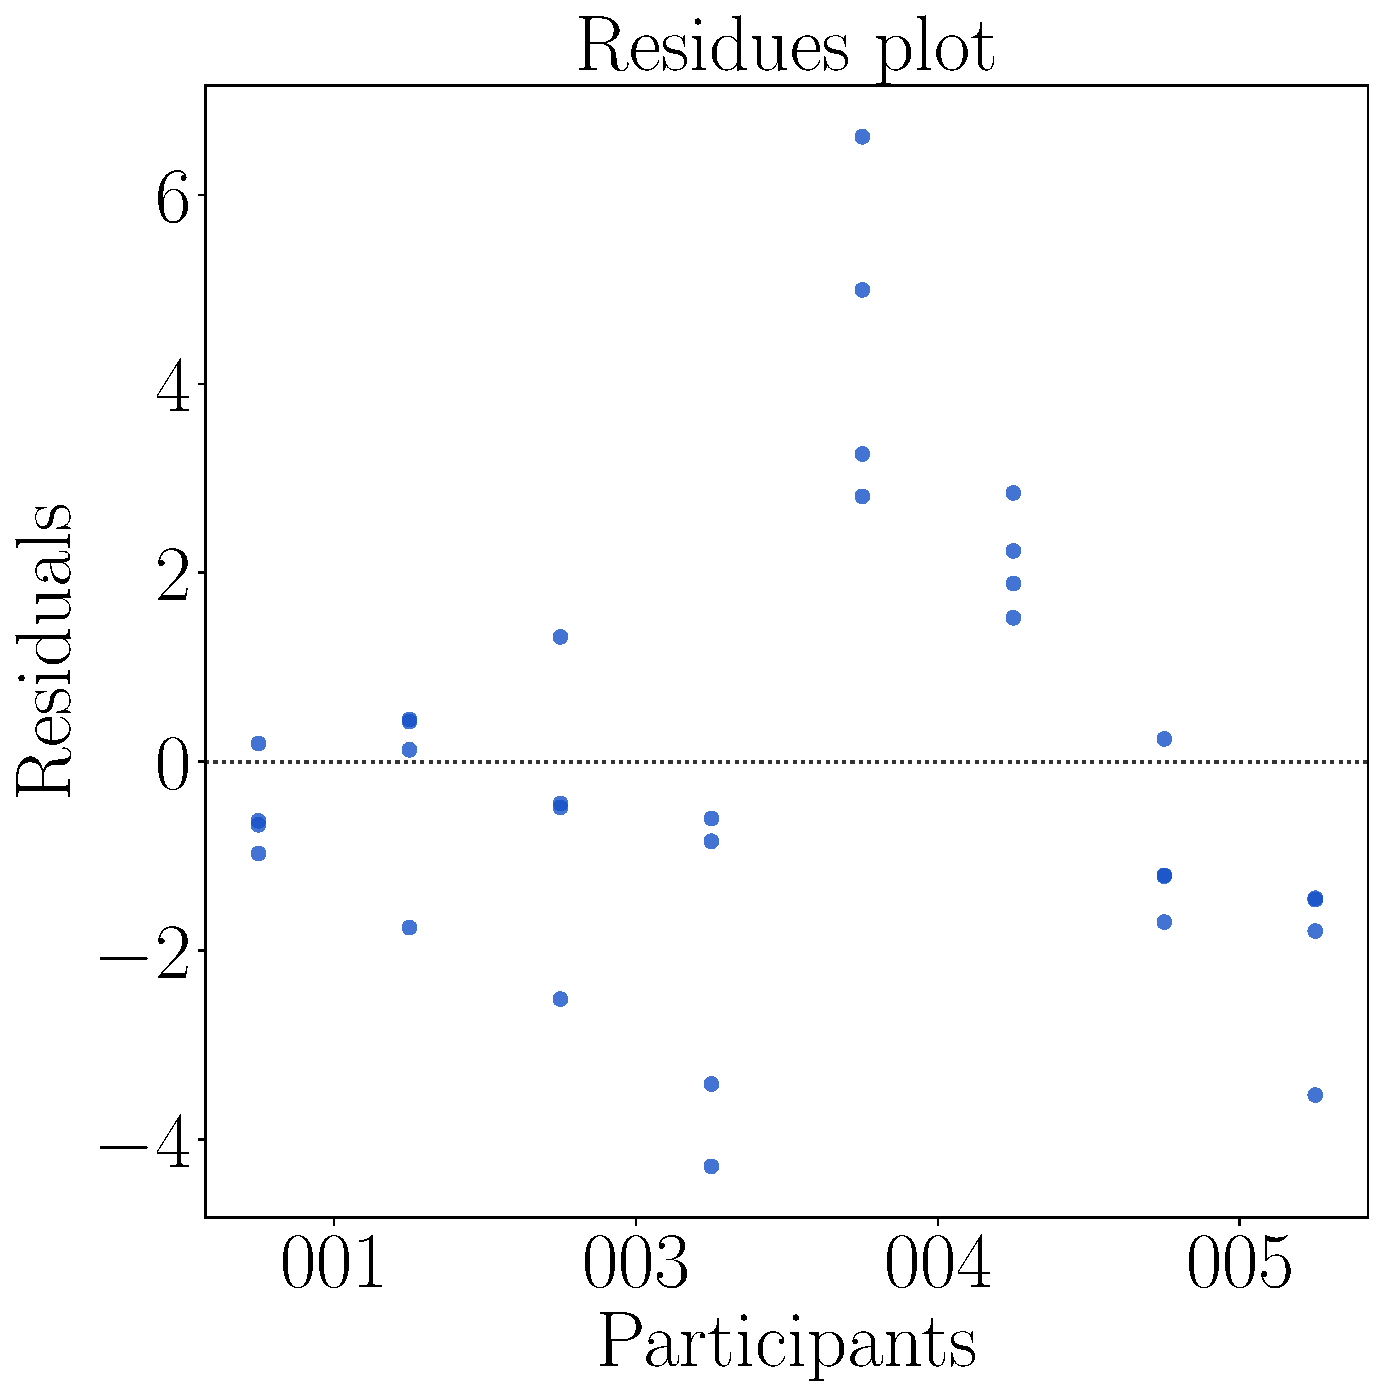
\includegraphics[width = \textwidth]{Resultados/Nasa/Figuras/pdf/residplot_nasa_avg_two_way_sight.pdf}
        \caption{Residual plot of the NASA-TLX score the sight participants on each method.}
        \label{fig:residplot_nasa_avg_two_way_sight}
    \end{minipage}
\end{figure}

\FloatBarrier

\subsubsection{Adapted SAGAT}
\label{subsubsec:results_adapted_sagat_2}

Table \ref{tab:sagat_table_noBase} presents the SAGAT score of all participants. The corresponding barplot is presented in Figure \ref{fig:barplot_sagat_avg_4_scene_blind_sight}.


\begin{table}[!htb]
\centering
\caption{SAGAT global score felled by the participants.}
\label{tab:sagat_table_noBase}
\begin{tabular}{lllrrrrr}
\toprule
    &       &        &  Audio & \begin{tabular}[c]{@{}l@{}}Haptic\\ Belt\end{tabular} & \begin{tabular}[c]{@{}l@{}}Virtual\\ Cane\end{tabular} & Mixture \\
Participant & \begin{tabular}[c]{@{}l@{}}Visual\\ Condition\end{tabular} & Round &        &                                                       &                                                        &         \\
\midrule
001C & Blind & First &  5.500 &                                                 5.330 &                                                  5.830 &   3.500 \\
    &       & Return &  6.500 &                                                 8.500 &                                                  5.500 &   5.500 \\
002C & Blind & First &  4.500 &                                                 3.990 &                                                  4.500 &   6.250 \\
    &       & Return &  5.000 &                                                 4.000 &                                                  6.500 &   8.500 \\
003C & Blind & First &  7.500 &                                                 7.490 &                                                  4.660 &   9.000 \\
    &       & Return & 10.000 &                                                 8.500 &                                                  9.000 &   9.000 \\
004C & Blind & First &  6.000 &                                                 7.660 &                                                  4.990 &   6.500 \\
    &       & Return &  6.000 &                                                 9.250 &                                                  7.250 &   9.000 \\
001 & Sight & First &  4.500 &                                                 4.330 &                                                  2.660 &   6.500 \\
    &       & Return &  6.000 &                                                 5.000 &                                                  5.000 &   4.500 \\
003 & Sight & First &  6.750 &                                                 5.990 &                                                  3.990 &   6.750 \\
    &       & Return &  6.000 &                                                 7.250 &                                                  6.250 &   7.500 \\
004 & Sight & First &  7.250 &                                                 7.990 &                                                  5.990 &   8.250 \\
    &       & Return &  7.750 &                                                 9.500 &                                                  8.250 &   7.000 \\
005 & Sight & First &  3.000 &                                                 3.160 &                                                  3.990 &   4.000 \\
    &       & Return &  3.750 &                                                 3.000 &                                                  2.000 &   6.000 \\
\bottomrule
\end{tabular}
\end{table}



Figure \ref{fig:barplot_sagat_avg_4_scene_blind_sight}. shows that the SAGAT score for sighted participants is on average lower than that of blind participants, which is expected as they are not used to navigate without vision. Also, the increase in situation awareness from the first to the return round is lower. In the case of the mixture method, the SAGAT score did not improve at all. For both groups, the ‘virtual cane’ was the method with lowest score in the first round.

\begin{figure}[!htb]
    \centering
    \begin{minipage}{\textwidth}
        \centering
        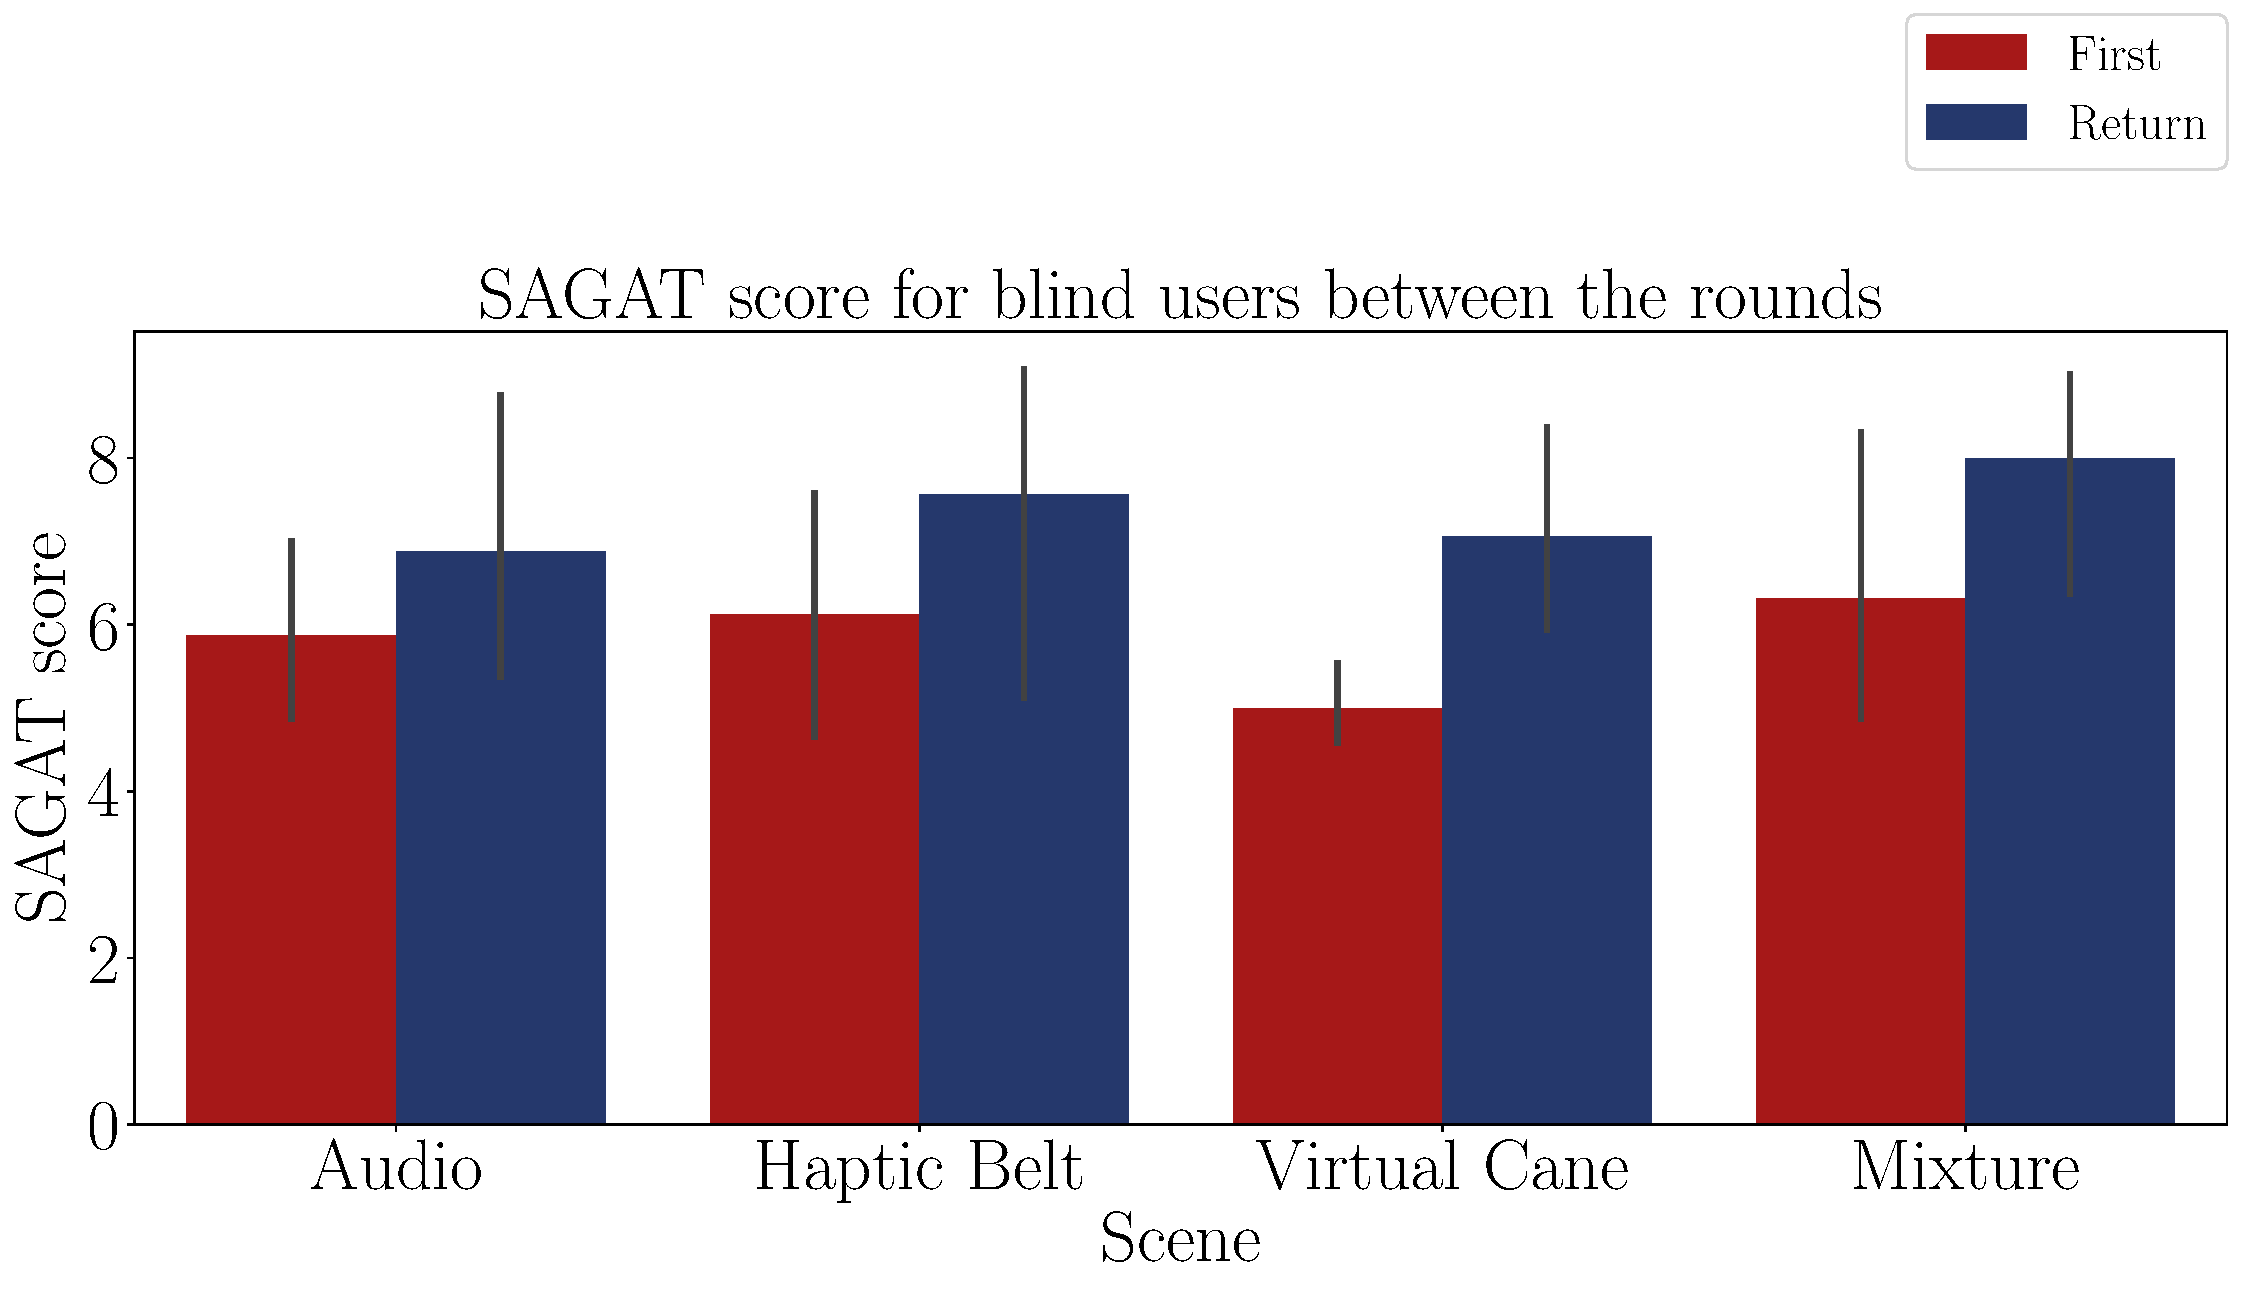
\includegraphics[width = \textwidth]{Resultados/Sagat/Figuras/pdf/barplot_sagat_avg_4_scene_blind.pdf}
        \subcaption{Blind participants.}
        \label{fig:barplot_sagat_avg_4_scene_blind}
    \end{minipage}
    \begin{minipage}{\textwidth}
        \centering
        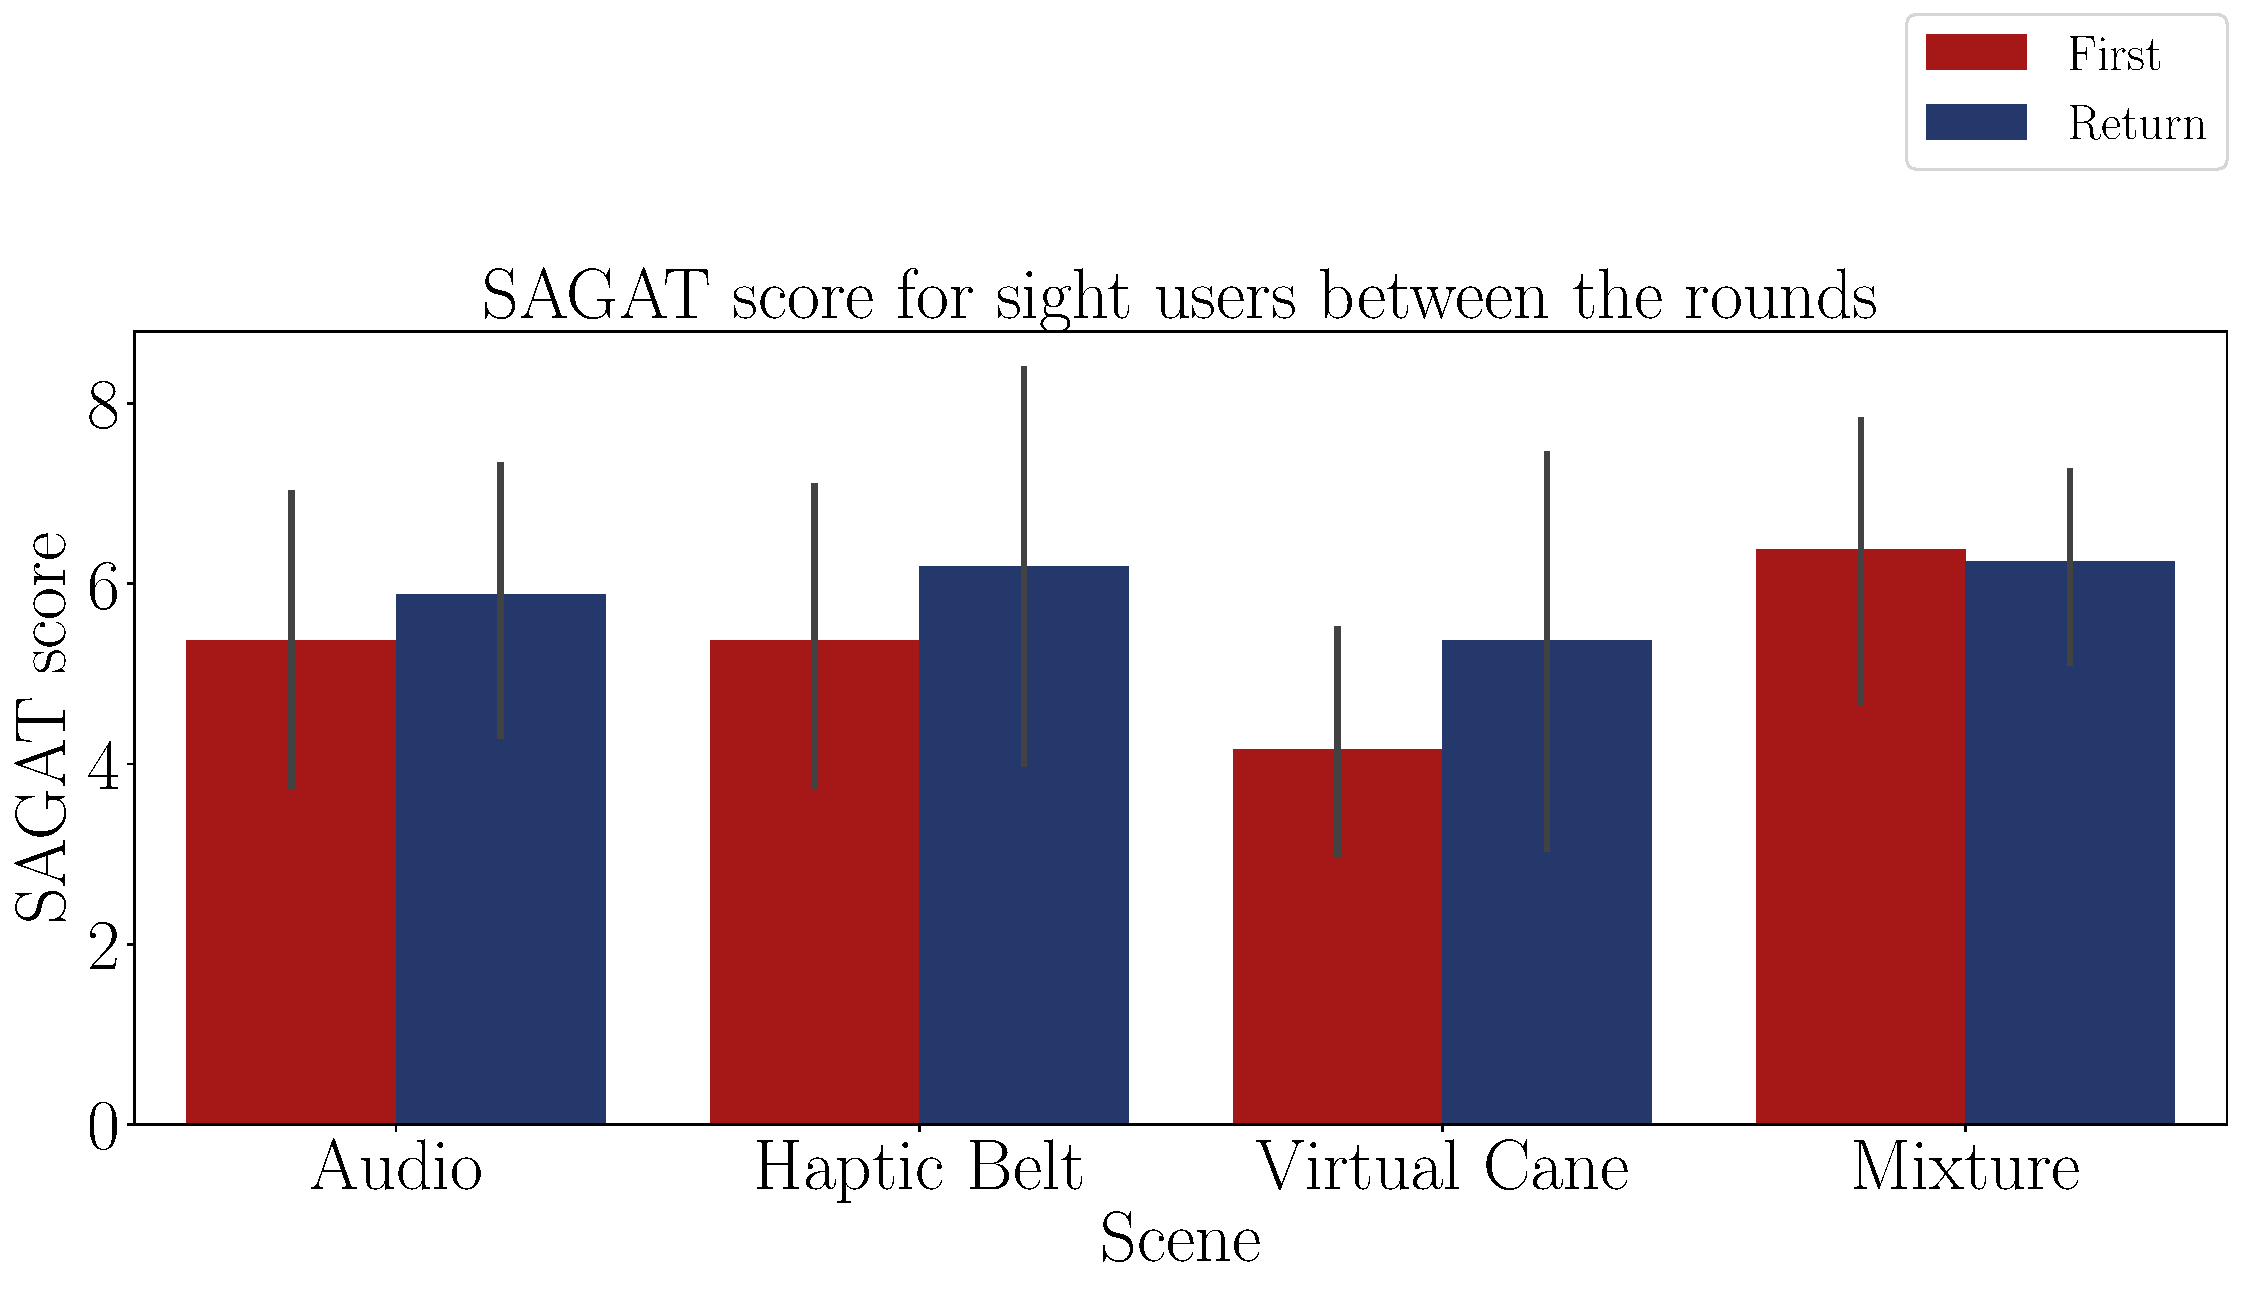
\includegraphics[width = \textwidth]{Resultados/Sagat/Figuras/pdf/barplot_sagat_avg_4_scene_sight.pdf}
        \subcaption{Sight participants.}
        \label{fig:barplot_sagat_avg_4_scene_sight}
    \end{minipage}
    \caption{Barplot of the SAGAT score on each method and round.}
    \label{fig:barplot_sagat_avg_4_scene_blind_sight}
\end{figure}

Figures \ref{fig:boxplot_sagat_4_scene} and \ref{fig:boxplot_sagat_4_rounds} bring the boxplots. According to Figure \ref{fig:boxplot_sagat_4_scene}, both groups presented a higher situation awareness with ‘mixture’ and ‘haptic’. On the other hand, Figure \ref{fig:boxplot_sagat_4_rounds} confirms that the difference between the rounds is greater for blind participants. 

\begin{figure}[!htb]
    \centering
    \begin{minipage}{0.45\textwidth}
        \centering
        \includegraphics[width = \textwidth]{Resultados/Sagat/Figuras/pdf/boxplot_sagat_4_scene.pdf}
        \caption{Boxplot of the Sagat score of the participants grouped by method.}
        \label{fig:boxplot_sagat_4_scene}
    \end{minipage}
    \begin{minipage}{0.075\textwidth}
        \hfill
    \end{minipage}
    \begin{minipage}{0.45\textwidth}
        \centering
        \includegraphics[width = \linewidth]{Resultados/Sagat/Figuras/pdf/boxplot_sagat_4_rounds.pdf}
        \caption{Boxplot of the Sagat score of the participants grouped by round.}
        \label{fig:boxplot_sagat_4_rounds}
    \end{minipage}
\end{figure}

Figures \ref{fig:qqplot_sagat_avg_two_way_sight} and \ref{fig:residplot_sagat_avg_two_way_sight} brings the QQ plot and residual distribution. It is clear that the residuals variance is not equal among the participants. Table \ref{tab:blocanova_sagat_avg_two_way_blind_sight} brings the p-value from ANOVA. While for blind participants the round is a significant factor and the method is not, for sighted participants the result is the opposite, showing a significant influence of the method and not of the round.

\begin{table}[!htb]
    \caption{Anova p-value for the SAGAT score on each method}
    \label{tab:blocanova_sagat_avg_two_way_blind_sight}
\begin{minipage}{0.45\textwidth}
    \subcaption{Blind participants}
    
\centering
\begin{tabular}{ll}
\toprule
          Source & P-Value \\
\midrule
    \    Methods &   0.277 \\
     \    Rounds & 0.002** \\
\    Interaction &   0.834 \\
\bottomrule
\end{tabular}

\end{minipage}
\begin{minipage}{0.45\textwidth}
    \subcaption{Sight participants}
    
\centering
\begin{tabular}{ll}
\toprule
          Source & P-Value \\
\midrule
    \    Methods & 0.035** \\
     \    Rounds &   0.095 \\
\    Interaction &   0.578 \\
\bottomrule
\end{tabular}
    
\end{minipage}
\end{table}


\begin{figure}[!htb]
    \centering
    %\vspace{-15.0cm}
    \begin{minipage}{0.45\textwidth}
        \centering
        \includegraphics[width = \textwidth]{Resultados/Sagat/Figuras/pdf/qqplot_sagat_avg_two_way_sight.pdf}
        \caption{QQ plot of the mental demand of the sight participants on each method.}
        \label{fig:qqplot_sagat_avg_two_way_sight}
    \end{minipage}
    \begin{minipage}{0.075\textwidth}
        \hfill
    \end{minipage}
    \begin{minipage}{0.45\textwidth}
        \centering
        \includegraphics[width = \textwidth]{Resultados/Sagat/Figuras/pdf/residplot_sagat_avg_two_way_sight.pdf}
        \caption{Residual plot of the mental demand score the sight participants on each method.}
        \label{fig:residplot_sagat_avg_two_way_sight}
    \end{minipage}
\end{figure}

%%%%%%%%%%%%%%%%%%%%%%%%%%%%%%%%%%%%%%%%%%%%%%%%%%%%%

\FloatBarrier

\subsection{Subjective data}
\subsubsection{NASA-TLX}
\label{subsubsec:results_nasa_tlx_2}

\paragraph{Analysis of the mental demand scale}\mbox{}\\

The Table \ref{tab:md_table_noBase} presents the ‘mental demand’ score of all participants, while the corresponding barplot is presented in Figure \ref{fig:barplot_md_avg_4_scene_blind_sight}. It is interesting to observe that sighted people gave a higher score to audio, as they are not so familiar to use sounds as source of guidance.


\begin{table}[!htb]
\centering
\caption{Mental demand felled by the participants.}
\label{tab:md_table_noBase}
\begin{tabular}{lllrrrrr}
\toprule
    &       &        & Audio & \begin{tabular}[c]{@{}l@{}}Haptic\\ Belt\end{tabular} & \begin{tabular}[c]{@{}l@{}}Virtual\\ Cane\end{tabular} & Mixture \\
Participant & \begin{tabular}[c]{@{}l@{}}Visual\\ Condition\end{tabular} & Round &       &                                                       &                                                        &         \\
\midrule
001 & Sight & First &    12 &                                                    11 &                                                      5 &       9 \\
    &       & Return &    13 &                                                    13 &                                                      5 &      10 \\
001C & Blind & First &     1 &                                                    14 &                                                      3 &       6 \\
    &       & Return &     1 &                                                    10 &                                                      2 &       6 \\
002C & Blind & First &     1 &                                                     1 &                                                     10 &      12 \\
    &       & Return &     1 &                                                     1 &                                                     10 &       3 \\
003 & Sight & First &    18 &                                                    18 &                                                     16 &      10 \\
    &       & Return &    12 &                                                    15 &                                                     11 &       8 \\
003C & Blind & First &     5 &                                                     5 &                                                      8 &       1 \\
    &       & Return &     1 &                                                     1 &                                                      2 &       1 \\
004 & Sight & First &    17 &                                                    20 &                                                     12 &      20 \\
    &       & Return &    12 &                                                    15 &                                                     10 &      15 \\
004C & Blind & First &    10 &                                                    15 &                                                     10 &      10 \\
    &       & Return &    10 &                                                    14 &                                                      8 &      10 \\
005 & Sight & First &     4 &                                                    12 &                                                     10 &      13 \\
    &       & Return &     6 &                                                    10 &                                                      6 &      12 \\
\bottomrule
\end{tabular}
\end{table}



\begin{figure}[!thb]
    \centering
    \begin{minipage}{\textwidth}
        \centering
        \includegraphics[width = \textwidth]{Resultados/Nasa/Figuras/pdf/barplot_md_avg_4_scene_blind.pdf}
        \subcaption{Blind participants}
        \label{fig:barplot_md_avg_4_scene_blind}
    \end{minipage}
    \begin{minipage}{\textwidth}
        \centering
        \includegraphics[width = \textwidth]{Resultados/Nasa/Figuras/pdf/barplot_md_avg_4_scene_sight.pdf}
        \subcaption{Sight participants}
        \label{fig:barplot_md_avg_4_scene_sight}
    \end{minipage}
    \caption{Barplot of the average mental demand on each method and round.}
    \label{fig:barplot_md_avg_4_scene_blind_sight}
\end{figure}

Figures \ref{fig:boxplot_noBase_md_4_scene} and \ref{fig:boxplot_noBase_md_4_rounds} presents the box plot for both groups, organized by method and round. It is clear that the mental demand is systematically higher for sighted people, which is something expected. But while blind participants considered the ‘audio’ method less demanding, sighted participants gave preference to the virtual cane. For both groups, we observe a decrease in the mental demand.

\begin{figure}[!htb]
    \centering
    \begin{minipage}{0.45\textwidth}
        \centering
        \includegraphics[width = \textwidth]{Resultados/Nasa/Figuras/pdf/boxplot_noBase_md_4_scene.pdf}
        \caption{Boxplot of the mental demand of the participants grouped by method.}
        \label{fig:boxplot_noBase_md_4_scene}
    \end{minipage}
    \begin{minipage}{0.075\textwidth}
        \hfill
    \end{minipage}
    \begin{minipage}{0.45\textwidth}
        \centering
        \includegraphics[width = \textwidth]{Resultados/Nasa/Figuras/pdf/boxplot_noBase_md_4_rounds.pdf}
        \caption{Boxplot of the mental demand of the participants grouped by round.}
        \label{fig:boxplot_noBase_md_4_rounds}
    \end{minipage}
\end{figure}

Figures \ref{fig:qqplot_md_avg_two_way_sight} and \ref{fig:residplot_md_avg_two_way_sight} show the QQ plot and residual distribution for the sighted data, confirming that the data is normally distributed and participants have similar variance. Table \ref{tab:blocanova_md_avg_two_way_blind_sight} brings the results of ANOVA. Different from the blind participants, in the case of sighted ones, the p-value for ‘method’ is below the threshold of 0.05, confirming it as a significant variable for the mental demand. In the case of ‘round’, data from both sighted and blind participants resulted in the same p-value of 0.075, which is close to the traditional threshold of 0.05, but slightly higher. 

\begin{table}[!htb]
    \caption{Anova p-value for the mental demand average on each method'}
    \label{tab:blocanova_md_avg_two_way_blind_sight}
\begin{minipage}{0.45\textwidth}
    \subcaption{Blind participants}
    
\centering
\begin{tabular}{ll}
\toprule
          Source & P-Value \\
\midrule
    \    Methods &   0.170 \\
     \    Rounds &   0.075 \\
\    Interaction &   0.993 \\
\bottomrule
\end{tabular}

\end{minipage}
\begin{minipage}{0.45\textwidth}
    \subcaption{Sight participants}
    
\centering
\begin{tabular}{ll}
\toprule
          Source & P-Value \\
\midrule
    \    Methods & 0.049** \\
     \    Rounds &   0.075 \\
\    Interaction &   0.990 \\
\bottomrule
\end{tabular}
    
\end{minipage}
\end{table}

\begin{figure}[!htb]
    \centering
    %\vspace{-15.0cm}
    \begin{minipage}{0.45\textwidth}
        \centering
        \includegraphics[width = \textwidth]{Resultados/Nasa/Figuras/pdf/qqplot_md_avg_two_way_sight.pdf}
        \caption{QQ plot of the mental demand of the sight participants on each method.}
        \label{fig:qqplot_md_avg_two_way_sight}
    \end{minipage}
    \begin{minipage}{0.075\textwidth}
        \hfill
    \end{minipage}
    \begin{minipage}{0.45\textwidth}
        \centering
        \includegraphics[width = \textwidth]{Resultados/Nasa/Figuras/pdf/residplot_md_avg_two_way_sight.pdf}
        \caption{Residual plot of the mental demand score the sighted participants on each method.}
        \label{fig:residplot_md_avg_two_way_sight}
    \end{minipage}
\end{figure}

\FloatBarrier

%%%%%%%%%%%%%%%%%%%%%%%%%%%%%%%%%%%%%%%%%%%%%%%%%%%%%%%%%%%%%%%%%%%%%%%%%%%%
%%%%%%%%%%%%%%%%%%%%%%%%%%%%%%%%%%%%%%%%%%%%%%%%%%%%%%%%%%%%%%%%%%%%%%%%%%%%
%%%%%%%%%%%%%%%%%%%%%%%%%%%%%%%%%%%%%%%%%%%%%%%%%%%%%%%%%%%%%%%%%%%%%%%%%%%%
%%%%%%%%%%%%%%%%%%%%%%%%%%%%%%%%%%%%%%%%%%%%%%%%%%%%%%%%%%%%%%%%%%%%%%%%%%%%


\paragraph{Analysis of the NASA-TLX score}\mbox{}\\

Table \ref{tab:nasa_table_noBase} brings the NASA-TLX global score of all participants, while the corresponding barplot is presented in Figure \ref{fig:barplot_nasa_avg_4_scene}.


\begin{table}[!htb]
\centering
\caption{NASA-TLX score felled by the participants.}
\label{tab:nasa_table_noBase}
\begin{tabular}{lllrrrrr}
\toprule
    &       &        &  Audio & \begin{tabular}[c]{@{}l@{}}Haptic\\ Belt\end{tabular} & \begin{tabular}[c]{@{}l@{}}Virtual\\ Cane\end{tabular} & Mixture \\
Participant & \begin{tabular}[c]{@{}l@{}}Visual\\ Condition\end{tabular} & Round &        &                                                       &                                                        &         \\
\midrule
001 & Sight & First & 10.167 &                                                 9.833 &                                                  7.000 &   9.000 \\
    &       & Return & 11.000 &                                                10.833 &                                                  6.167 &   9.333 \\
001C & Blind & First &  4.000 &                                                 8.833 &                                                  5.167 &   6.333 \\
    &       & Return &  4.000 &                                                 6.667 &                                                  4.500 &   6.167 \\
002C & Blind & First &  4.833 &                                                 4.833 &                                                  9.000 &   7.000 \\
    &       & Return &  4.833 &                                                 4.833 &                                                  7.000 &   5.167 \\
003 & Sight & First &  9.833 &                                                10.167 &                                                  9.500 &   6.500 \\
    &       & Return &  6.667 &                                                 9.667 &                                                  7.833 &   4.833 \\
003C & Blind & First &  4.000 &                                                 5.333 &                                                  6.667 &   3.500 \\
    &       & Return &  3.833 &                                                 3.667 &                                                  3.500 &   3.500 \\
004 & Sight & First & 14.833 &                                                13.667 &                                                 11.500 &  15.833 \\
    &       & Return & 11.833 &                                                11.833 &                                                 10.833 &  12.167 \\
004C & Blind & First & 10.000 &                                                12.667 &                                                  9.667 &  11.000 \\
    &       & Return &  9.167 &                                                11.667 &                                                  9.333 &  10.833 \\
005 & Sight & First &  7.667 &                                                 9.000 &                                                  8.000 &   9.667 \\
    &       & Return &  7.667 &                                                 8.667 &                                                  7.667 &   6.000 \\
\bottomrule
\end{tabular}
\end{table}



From Figure \ref{fig:barplot_nasa_avg_4_scene} it is possible to see that, similar to blind participants, sighted participants also consider that the workload of the return round was lower than that of the first round. However, similar to what happened for the mental demand, sighted participants considered ‘virtual cane’ as the method with the lowest workload, while, for  blind participants, it was the ‘audio’.

\begin{figure}[!htb]
    \centering
    \begin{minipage}{\textwidth}
        \centering
        \includegraphics[width = \textwidth]{Resultados/Nasa/Figuras/pdf/barplot_nasa_avg_4_scene_blind.pdf}
        \subcaption{Blind participants.}
        \label{fig:barplot_nasa_avg_4_scene_blind}
    \end{minipage}
    \begin{minipage}{\textwidth}
        \centering
        \includegraphics[width = \textwidth]{Resultados/Nasa/Figuras/pdf/barplot_nasa_avg_4_scene_sight.pdf}
        \subcaption{Sight participants.}
        \label{fig:barplot_nasa_avg_4_scene_sight}
    \end{minipage}
    \caption{Barplot of the NASA-TLX score on each method and round.}
    \label{fig:barplot_nasa_avg_4_scene}
\end{figure}

Figures \ref{fig:boxplot_noBase_nasa_4_scene} and \ref{fig:boxplot_noBase_nasa_4_rounds} present the boxplots of NASA-TLX global score. Again, it is possible to see that sighted people usually give higher workload scores than blind ones. The influence of the round is approximately the same. But the order of preference of the methods are different.

\begin{figure}[!htb]
    \centering
    \begin{minipage}{0.45\textwidth}
        \centering
        \includegraphics[width = \textwidth]{Resultados/Nasa/Figuras/pdf/boxplot_noBase_nasa_4_scene.pdf}
        \caption{Boxplot of the NASA-TLX score of the participants grouped by method.}
        \label{fig:boxplot_noBase_nasa_4_scene}
    \end{minipage}
    \begin{minipage}{0.075\textwidth}
        \hfill
    \end{minipage}
    \begin{minipage}{0.45\textwidth}
        \centering
        \includegraphics[width = \textwidth]{Resultados/Nasa/Figuras/pdf/boxplot_noBase_nasa_4_rounds.pdf}
        \caption{Boxplot of the NASA-TLX score of the participants grouped by round.}
        \label{fig:boxplot_noBase_nasa_4_rounds}
    \end{minipage}
\end{figure}

Figures \ref{fig:qqplot_nasa_avg_two_way_sight} and \ref{fig:residplot_nasa_avg_two_way_sight} bring the QQ plot and residual distribution of the data from sighted participants, showing that ANOVA can be used. The p-values for both groups are presented in Table \ref{tab:blocanova_nasa_avg_two_way_blind_sight}. It confirms the influence of the round for both sighted and blind people. In the case of the method, the p-value of ‘blind’ is lower than the threshold of 0.5, while that of ‘sighted’ is slightly higher.

\begin{table}[!thb]
    \caption{Anova p-value for the NASA-TLX score on each method}
    \label{tab:blocanova_nasa_avg_two_way_blind_sight}
    \begin{minipage}{0.45\textwidth}
        \subcaption{Blind participants}
        
\centering
\begin{tabular}{ll}
\toprule
          Source & P-Value \\
\midrule
    \    Methods & 0.029** \\
     \    Rounds & 0.022** \\
\    Interaction &   0.814 \\
\bottomrule
\end{tabular}

    \end{minipage}
    \begin{minipage}{0.45\textwidth}
        \subcaption{Sight participants}
        
\centering
\begin{tabular}{ll}
\toprule
          Source & P-Value \\
\midrule
    \    Methods &   0.086 \\
     \    Rounds & 0.034** \\
\    Interaction &   0.688 \\
\bottomrule
\end{tabular}
    
    \end{minipage}
\end{table}


\begin{figure}[!htb]
    \centering
    %\vspace{-15.0cm}
    \begin{minipage}{0.45\textwidth}
        \centering
        \includegraphics[width = \textwidth]{Resultados/Nasa/Figuras/pdf/qqplot_nasa_avg_two_way_sight.pdf}
        \caption{QQ plot of the NASA-TLX score of the sight participants on each method.}
        \label{fig:qqplot_nasa_avg_two_way_sight}
    \end{minipage}
    \begin{minipage}{0.075\textwidth}
        \hfill
    \end{minipage}
    \begin{minipage}{0.45\textwidth}
        \centering
        \includegraphics[width = \textwidth]{Resultados/Nasa/Figuras/pdf/residplot_nasa_avg_two_way_sight.pdf}
        \caption{Residual plot of the NASA-TLX score the sight participants on each method.}
        \label{fig:residplot_nasa_avg_two_way_sight}
    \end{minipage}
\end{figure}

\FloatBarrier
\subsubsection{Adapted SAGAT}
\label{subsubsec:results_adapted_sagat_2}

Table \ref{tab:sagat_table_noBase} presents the SAGAT score of all participants. The corresponding barplot is presented in Figure \ref{fig:barplot_sagat_avg_4_scene_blind_sight}.


\begin{table}[!htb]
\centering
\caption{SAGAT global score felled by the participants.}
\label{tab:sagat_table_noBase}
\begin{tabular}{lllrrrrr}
\toprule
    &       &        &  Audio & \begin{tabular}[c]{@{}l@{}}Haptic\\ Belt\end{tabular} & \begin{tabular}[c]{@{}l@{}}Virtual\\ Cane\end{tabular} & Mixture \\
Participant & \begin{tabular}[c]{@{}l@{}}Visual\\ Condition\end{tabular} & Round &        &                                                       &                                                        &         \\
\midrule
001C & Blind & First &  5.500 &                                                 5.330 &                                                  5.830 &   3.500 \\
    &       & Return &  6.500 &                                                 8.500 &                                                  5.500 &   5.500 \\
002C & Blind & First &  4.500 &                                                 3.990 &                                                  4.500 &   6.250 \\
    &       & Return &  5.000 &                                                 4.000 &                                                  6.500 &   8.500 \\
003C & Blind & First &  7.500 &                                                 7.490 &                                                  4.660 &   9.000 \\
    &       & Return & 10.000 &                                                 8.500 &                                                  9.000 &   9.000 \\
004C & Blind & First &  6.000 &                                                 7.660 &                                                  4.990 &   6.500 \\
    &       & Return &  6.000 &                                                 9.250 &                                                  7.250 &   9.000 \\
001 & Sight & First &  4.500 &                                                 4.330 &                                                  2.660 &   6.500 \\
    &       & Return &  6.000 &                                                 5.000 &                                                  5.000 &   4.500 \\
003 & Sight & First &  6.750 &                                                 5.990 &                                                  3.990 &   6.750 \\
    &       & Return &  6.000 &                                                 7.250 &                                                  6.250 &   7.500 \\
004 & Sight & First &  7.250 &                                                 7.990 &                                                  5.990 &   8.250 \\
    &       & Return &  7.750 &                                                 9.500 &                                                  8.250 &   7.000 \\
005 & Sight & First &  3.000 &                                                 3.160 &                                                  3.990 &   4.000 \\
    &       & Return &  3.750 &                                                 3.000 &                                                  2.000 &   6.000 \\
\bottomrule
\end{tabular}
\end{table}



Figure \ref{fig:barplot_sagat_avg_4_scene_blind_sight}. shows that the SAGAT score for sighted participants is on average lower than that of blind participants, which is expected as they are not used to navigate without vision. Also, the increase in situation awareness from the first to the return round is lower. In the case of the mixture method, the SAGAT score did not improve at all. For both groups, the ‘virtual cane’ was the method with lowest score in the first round.

\begin{figure}[!htb]
    \centering
    \begin{minipage}{\textwidth}
        \centering
        \includegraphics[width = \textwidth]{Resultados/Sagat/Figuras/pdf/barplot_sagat_avg_4_scene_blind.pdf}
        \subcaption{Blind participants.}
        \label{fig:barplot_sagat_avg_4_scene_blind}
    \end{minipage}
    \begin{minipage}{\textwidth}
        \centering
        \includegraphics[width = \textwidth]{Resultados/Sagat/Figuras/pdf/barplot_sagat_avg_4_scene_sight.pdf}
        \subcaption{Sight participants.}
        \label{fig:barplot_sagat_avg_4_scene_sight}
    \end{minipage}
    \caption{Barplot of the SAGAT score on each method and round.}
    \label{fig:barplot_sagat_avg_4_scene_blind_sight}
\end{figure}

Figures \ref{fig:boxplot_sagat_4_scene} and \ref{fig:boxplot_sagat_4_rounds} bring the boxplots. According to Figure \ref{fig:boxplot_sagat_4_scene}, both groups presented a higher situation awareness with ‘mixture’ and ‘haptic’. On the other hand, Figure \ref{fig:boxplot_sagat_4_rounds} confirms that the difference between the rounds is greater for blind participants. 

\begin{figure}[!htb]
    \centering
    \begin{minipage}{0.45\textwidth}
        \centering
        \includegraphics[width = \textwidth]{Resultados/Sagat/Figuras/pdf/boxplot_sagat_4_scene.pdf}
        \caption{Boxplot of the Sagat score of the participants grouped by method.}
        \label{fig:boxplot_sagat_4_scene}
    \end{minipage}
    \begin{minipage}{0.075\textwidth}
        \hfill
    \end{minipage}
    \begin{minipage}{0.45\textwidth}
        \centering
        \includegraphics[width = \linewidth]{Resultados/Sagat/Figuras/pdf/boxplot_sagat_4_rounds.pdf}
        \caption{Boxplot of the Sagat score of the participants grouped by round.}
        \label{fig:boxplot_sagat_4_rounds}
    \end{minipage}
\end{figure}

Figures \ref{fig:qqplot_sagat_avg_two_way_sight} and \ref{fig:residplot_sagat_avg_two_way_sight} brings the QQ plot and residual distribution. It is clear that the residuals variance is not equal among the participants. Table \ref{tab:blocanova_sagat_avg_two_way_blind_sight} brings the p-value from ANOVA. While for blind participants the round is a significant factor and the method is not, for sighted participants the result is the opposite, showing a significant influence of the method and not of the round.

\begin{table}[!htb]
    \caption{Anova p-value for the SAGAT score on each method}
    \label{tab:blocanova_sagat_avg_two_way_blind_sight}
\begin{minipage}{0.45\textwidth}
    \subcaption{Blind participants}
    
\centering
\begin{tabular}{ll}
\toprule
          Source & P-Value \\
\midrule
    \    Methods &   0.277 \\
     \    Rounds & 0.002** \\
\    Interaction &   0.834 \\
\bottomrule
\end{tabular}

\end{minipage}
\begin{minipage}{0.45\textwidth}
    \subcaption{Sight participants}
    
\centering
\begin{tabular}{ll}
\toprule
          Source & P-Value \\
\midrule
    \    Methods & 0.035** \\
     \    Rounds &   0.095 \\
\    Interaction &   0.578 \\
\bottomrule
\end{tabular}
    
\end{minipage}
\end{table}


\begin{figure}[!htb]
    \centering
    %\vspace{-15.0cm}
    \begin{minipage}{0.45\textwidth}
        \centering
        \includegraphics[width = \textwidth]{Resultados/Sagat/Figuras/pdf/qqplot_sagat_avg_two_way_sight.pdf}
        \caption{QQ plot of the mental demand of the sight participants on each method.}
        \label{fig:qqplot_sagat_avg_two_way_sight}
    \end{minipage}
    \begin{minipage}{0.075\textwidth}
        \hfill
    \end{minipage}
    \begin{minipage}{0.45\textwidth}
        \centering
        \includegraphics[width = \textwidth]{Resultados/Sagat/Figuras/pdf/residplot_sagat_avg_two_way_sight.pdf}
        \caption{Residual plot of the mental demand score the sight participants on each method.}
        \label{fig:residplot_sagat_avg_two_way_sight}
    \end{minipage}
\end{figure}

%%%%%%%%%%%%%%%%%%%%%%%%%%%%%%%%%%%%%%%%%%%%%%%%%%%%%

\FloatBarrier
\subsubsection{Guidance method's questionnaire.}
\label{subsubsec:results_questionnaires_2}

As for the blind users, the sighted user also answered the Guidance questionnaire to give their thoughts about their experience with the guidance methods. Table \ref{tab:questionnaire_average} shows the score of both groups. As said before, the higher the value, the higher is the user satisfaction. The corresponding barplots are presented in Figure \ref{fig:barplot_questionnaire_scene_blind_sight}. Both groups prefer audio  and mixture methods. The difference lies in the preference between the haptic belt and virtual cane. The blind users tend to prefer the first one, while the sighted users tend to prefer the last.


\begin{table}[!htb]
\centering
\caption{Guidance method questionnaire average score grouped by participant.}
\label{tab:questionnaire_average}
\begin{tabular}{lllrrrrr}
\toprule
{} & Audio & \begin{tabular}[c]{@{}l@{}}Haptic\\ Belt\end{tabular} & \begin{tabular}[c]{@{}l@{}}Virtual\\ Cane\end{tabular} & Mixture & Visual Condition \\
Participant &       &                                                       &                                                        &         &                  \\
\midrule
001         &  0.75 &                                                  0.49 &                                                   0.57 &    0.69 &            Sight \\
001C        &  0.77 &                                                  0.54 &                                                   0.63 &    0.87 &            Blind \\
002C        &  0.86 &                                                  0.74 &                                                   0.54 &    0.93 &            Blind \\
003         &  0.76 &                                                  0.54 &                                                   0.54 &    0.78 &            Sight \\
003C        &  0.93 &                                                  0.57 &                                                   0.54 &    0.74 &            Blind \\
004         &  0.86 &                                                  0.60 &                                                   0.79 &    0.76 &            Sight \\
004C        &  0.88 &                                                  0.49 &                                                   0.40 &    0.73 &            Blind \\
005         &  0.61 &                                                  0.57 &                                                   0.75 &    0.84 &            Sight \\
\bottomrule
\end{tabular}
\end{table}



\begin{figure}[!htb]
    \centering
    \begin{minipage}{\textwidth}
        \centering
        \includegraphics[width = \textwidth]{Resultados/Questionario/Figuras/pdf/barplot_questionnaire_scene_blind.pdf}
        \subcaption{Blind participants.}
        \label{fig:barplot_questionnaire_scene_blind_2}
    \end{minipage}
    \begin{minipage}{\textwidth}
        \centering
        \includegraphics[width = \textwidth]{Resultados/Questionario/Figuras/pdf/barplot_questionnaire_scene_sight.pdf}
        \subcaption{Sighted participants.}
        \label{fig:barplot_questionnaire_scene_sight}
    \end{minipage}
    \caption{Barplot of the average questionaire score on each method.}
    \label{fig:barplot_questionnaire_scene_blind_sight}
\end{figure}
%\begin{figure}[!htb]
%    \centering
%    \includegraphics[width = \textwidth]{Resultados/Questionario/Figuras/png/barplot_questionnaire_scene.png}
%    \caption{Barplot of the  average questionaire score of both participants on each method.}
%    \label{fig:barplot_questionnaire_scene}
%\end{figure}

The Figure \ref{fig:boxplot_questionnaire_scene} presents the box plot with the distribution of the scores. It is possible to see that there is some similarity between the two groups, except for the virtual cane method, which has a broader distribution for the sighted users. Also, it seems that the audio and mixture have similar acceptance for sighted and blind users.

\begin{figure}[!htb]
    \centering
    \includegraphics[width = 0.45\textwidth]{Resultados/Questionario/Figuras/pdf/boxplot_questionnaire_scene.pdf}
    \caption{Boxplot of the questionaire score of the the participants grouped by the methods.}
    \label{fig:boxplot_questionnaire_scene}
\end{figure}

%The Table \ref{tab:questionnaire_average_group} show the the average questionnaire score on each method of both groups and it shows the same conclusion as the Figure \ref{fig:barplot_questionnaire_scene}, that the preference between the "Haptic Belt" and "Virtual Cane" is the only difference between the two groups.
%
%Considering the most preferable and the less preferable of each group, the blind users are score their choices more intesiver than the sighted users. This may be an effect from their previous experience with the "Audio" method in previous events before the experiment and with haptic devices were something very, or almost, new. For the sighted users everything was new, so there scores were more consistent. This is posible to see in the average and standar deviation of these scores. For the blind users is 0.7 and 0.164 and for the sighted user is 0.682 and 0.100.
%
%
\begin{table}[!htb]
\centering
\caption{Guidance method questionnaire average score grouped by visual condition.}
\label{tab:questionnaire_average_group}
\begin{tabular}{lllll}
\toprule
{} &  Audio &  Haptic Belt &  Virtual Cane &  Mixture \\
Visual Condition &        &              &               &          \\
\midrule
Blind            &  0.693 &        0.757 &         0.471 &    0.735 \\
Sight            &  0.674 &        0.707 &         0.571 &    0.698 \\
\bottomrule
\end{tabular}
\end{table}



Figures \ref{fig:qqplot_questionnaire_sight} and \ref{fig:residplot_questionnaire_sight} brings the QQ plot and residual distribution, which confirm that ANOVA can be applied. The result of ANOVA is presented in Table \ref{tab:blocanova_questionnaire_blind_sight} and indicates that the method is an effective variable for the sighted participants, as it is for the blind ones.

\begin{table}[!htb]
    \caption{Anova p-value for the questionnaire score on each method}
    \label{tab:blocanova_questionnaire_blind_sight}
\begin{minipage}{0.45\textwidth}
    \subcaption{Blind participants.}
    
\centering
\begin{tabular}{ll}
\toprule
Source & P-Value \\
\midrule
Method & 0.001** \\
\bottomrule
\end{tabular}

\end{minipage}
\begin{minipage}{0.45\textwidth}
    \subcaption{Sight participants.}
    
\centering
\begin{tabular}{ll}
\toprule
Source & P-Value \\
\midrule
Method & 0.016** \\
\bottomrule
\end{tabular}

\end{minipage}
\end{table}

\begin{figure}[!htb]
    \centering
    %\vspace{-15.0cm}
    \begin{minipage}{0.45\textwidth}
        \centering
        \includegraphics[width = \textwidth]{Resultados/Questionario/Figuras/pdf/qqplot_questionnaire_sight.pdf}
        \caption{QQ plot of the questionnaire score of the sighted participants on each method.}
        \label{fig:qqplot_questionnaire_sight}
    \end{minipage}
    \begin{minipage}{0.075\textwidth}
        \hfill
    \end{minipage}
    \begin{minipage}{0.45\textwidth}
        \centering
        \includegraphics[width = \textwidth]{Resultados/Questionario/Figuras/pdf/residplot_questionnaire_sight.pdf}
        \caption{Residual plot of the questionnaire score the sighted participants on each method.}
        \label{fig:residplot_questionnaire_sight}
    \end{minipage}
\end{figure}

Table \ref{tab:lsd_questionnaire_blind_sight} presents the conclusion of a pairwise Fisher LSD test between all the guidance methods for both groups, showing that the results are coincident.

\FloatBarrier

\begin{table}[!thb]
    \caption{Anova p-value for the mental demand average on each method'}
    \label{tab:lsd_questionnaire_blind_sight}
    \begin{minipage}{1\textwidth}
        \subcaption{Blind participants.}
        
\centering
\begin{tabular}{rclr}
\toprule
      \multicolumn{3}{c}{Method} &                                           Analysis \\
\midrule
       Audio & $X$ & Haptic Belt &        $H_1 : \mu_{Audio} \ne \mu_{Haptic Belt}**$ \\
      Audio & $X$ & Virtual Cane &       $H_1 : \mu_{Audio} \ne \mu_{Virtual Cane}**$ \\
           Audio & $X$ & Mixture &                $H_0 : \mu_{Audio} = \mu_{Mixture}$ \\
Haptic Belt & $X$ & Virtual Cane & $H_1 : \mu_{Haptic Belt} \ne \mu_{Virtual Cane}**$ \\
     Haptic Belt & $X$ & Mixture &      $H_1 : \mu_{Haptic Belt} \ne \mu_{Mixture}**$ \\
    Virtual Cane & $X$ & Mixture &     $H_1 : \mu_{Virtual Cane} \ne \mu_{Mixture}**$ \\
\bottomrule
\end{tabular}

    \end{minipage}
    \begin{minipage}{1\textwidth}
        \subcaption{Sight participants.}
        
\centering
\begin{tabular}{rclr}
\toprule
      \multicolumn{3}{c}{Method} &                                           Analysis \\
\midrule
       Audio & $X$ & Haptic Belt &        $H_1 : \mu_{Audio} \ne \mu_{Haptic Belt}**$ \\
      Audio & $X$ & Virtual Cane &       $H_1 : \mu_{Audio} \ne \mu_{Virtual Cane}**$ \\
           Audio & $X$ & Mixture &                $H_0 : \mu_{Audio} = \mu_{Mixture}$ \\
Haptic Belt & $X$ & Virtual Cane & $H_1 : \mu_{Haptic Belt} \ne \mu_{Virtual Cane}**$ \\
     Haptic Belt & $X$ & Mixture &      $H_1 : \mu_{Haptic Belt} \ne \mu_{Mixture}**$ \\
    Virtual Cane & $X$ & Mixture &     $H_1 : \mu_{Virtual Cane} \ne \mu_{Mixture}**$ \\
\bottomrule
\end{tabular}

    \end{minipage}
\end{table}

%
\begin{table}[!htb]
\centering
\caption{Cross validation p-value for the questionnaire score on each method for blinded users.}
\label{tab:lsd_questionnaire}
\begin{tabular}{rclr}
\toprule
      \multicolumn{3}{c}{Method} &                                           Analysis \\
\midrule
       Audio & $X$ & Haptic Belt &        $H_1 : \mu_{Audio} \ne \mu_{Haptic Belt}**$ \\
      Audio & $X$ & Virtual Cane &       $H_1 : \mu_{Audio} \ne \mu_{Virtual Cane}**$ \\
           Audio & $X$ & Mixture &                $H_0 : \mu_{Audio} = \mu_{Mixture}$ \\
Haptic Belt & $X$ & Virtual Cane & $H_1 : \mu_{Haptic Belt} \ne \mu_{Virtual Cane}**$ \\
     Haptic Belt & $X$ & Mixture &          $H_0 : \mu_{Haptic Belt} = \mu_{Mixture}$ \\
    Virtual Cane & $X$ & Mixture &     $H_1 : \mu_{Virtual Cane} \ne \mu_{Mixture}**$ \\
\bottomrule
\end{tabular}
\end{table}



%The LSD Table \ref{tab:lsd_questionnaire_sight} repeat the same conclusion of the blind participants, that only the "Audio" and "Mixture" are statistically the same. But that does not mean that both groups had the same opinion from the rest of the methods. As shown in the Figure \ref{fig:boxplot_questionnaire_scene}, the average sighted user rather use the "Virtual Cane" then the "Haptic Belt", despite that distribution being wider, hence more varied, meaning that this is hardly a consense between the users.

%\FloatBarrier

\subsection{Physiological data}

\subsubsection{Electrocardiogram (ECG) data}
\label{subsubsec:results_ecg_2}

\paragraph{Analysis of the heartbeat frequency (BPM)}\mbox{}\\

Table \ref{tab:bpm_table_noBase} presents the average heart rate for both sighted and blind groups. The barplots are presented in Figure \ref{fig:barplot_ecg_bpm_4_scene_blind_sight}. Comparing the two groups, the audio method is associated with a slightly lower heartrate for blind people, but the opposite happens for sighted participants. Moreover, data from blind participants have large variance. This large variance can also be observed in the boxplot of Figures \ref{fig:boxplot_ecg_bpm_4_scene} and \ref{fig:boxplot_ecg_bpm_4_rounds}. 


\begin{table}[!htb]
\centering
\caption{ECG average BPM felled by the participants using the proposed methods [BPM].}
\label{tab:bpm_table_noBase}
\begin{tabular}{lllrrrrr}
\toprule
    &       &        &  Audio & \begin{tabular}[c]{@{}l@{}}Haptic\\ Belt\end{tabular} & \begin{tabular}[c]{@{}l@{}}Virtual\\ Cane\end{tabular} & Mixture \\
Part. & \begin{tabular}[c]{@{}l@{}}Visual\\ Condition\end{tabular} & Round &        &                                                       &                                                        &         \\
\midrule
001 & Sight & First &  71.23 &                                                 63.02 &                                                  64.85 &   58.77 \\
    &       & Return &  73.18 &                                                 61.18 &                                                  66.78 &   66.26 \\
001C & Blind & First &  60.71 &                                                 71.17 &                                                  59.07 &   68.24 \\
    &       & Return &  58.61 &                                                 66.22 &                                                  64.20 &   70.76 \\
002C & Blind & First &  38.67 &                                                 48.74 &                                                  46.89 &   52.23 \\
    &       & Return &  47.58 &                                                 58.97 &                                                  56.75 &   58.25 \\
003 & Sight & First &  63.47 &                                                 71.80 &                                                  70.90 &   72.76 \\
    &       & Return &  72.75 &                                                 71.23 &                                                  67.49 &   73.01 \\
003C & Blind & First &  69.89 &                                                 70.95 &                                                  69.41 &   66.94 \\
    &       & Return &  67.44 &                                                 69.68 &                                                  68.82 &   67.37 \\
004 & Sight & First &  66.85 &                                                 62.45 &                                                  65.94 &   67.86 \\
    &       & Return &  69.48 &                                                 65.65 &                                                  64.58 &   71.86 \\
004C & Blind & First &  73.55 &                                                 73.70 &                                                  71.94 &   74.03 \\
    &       & Return &  74.79 &                                                 74.02 &                                                  72.69 &   67.34 \\
005 & Sight & First &  71.34 &                                                 66.93 &                                                  66.46 &   67.06 \\
    &       & Return &  69.57 &                                                 65.97 &                                                  67.00 &   65.47 \\
\bottomrule
\end{tabular}
\end{table}



\begin{figure}[!htpb]
    \centering
    \begin{minipage}{\textwidth}
        \centering
        \includegraphics[width = 0.8\linewidth]{Resultados/ECG/Figuras/pdf/barplot_ecg_bpm_4_scene_blind.pdf}
        \subcaption{Blind participants.}
        \label{fig:barplot_ecg_bpm_4_scene_blind}
    \end{minipage}
    \begin{minipage}{\textwidth}
        \centering
        \includegraphics[width = 0.8\linewidth]{Resultados/ECG/Figuras/pdf/barplot_ecg_bpm_4_scene_sight.pdf}
        \subcaption{Sight participants.}
        \label{fig:barplot_ecg_bpm_4_scene_sight}
    \end{minipage}
    \caption{Barplot of the average BPM of the on each ethod and round.}
    \label{fig:barplot_ecg_bpm_4_scene_blind_sight}
\end{figure}
%\begin{figure}[!htpb]
%    \centering
%    \includegraphics[width = 0.8\linewidth]{Resultados/ECG/Figuras/pdf/barplot_ecg_bpm_4_scene.pdf}
%    \caption{Barplot of the average BPM of both participants on each method.}
%    \label{fig:barplot_ecg_bpm_4_scene}
%\end{figure}

\begin{figure}[!htpb]
    \centering
    \begin{minipage}{0.45\textwidth}
        \centering
        \includegraphics[width = 0.8\linewidth]{Resultados/ECG/Figuras/pdf/boxplot_ecg_bpm_4_scene.pdf}
        \caption{Boxplot of the average BPM of the participants grouped by method.}
        \label{fig:boxplot_ecg_bpm_4_scene}
    \end{minipage}
    \begin{minipage}{0.075\textwidth}
        \hfill
    \end{minipage}
    \begin{minipage}{0.45\textwidth}
        \centering
        \includegraphics[width = 0.8\linewidth]{Resultados/ECG/Figuras/pdf/boxplot_ecg_bpm_4_rounds.pdf}
        \caption{Boxplot of the average BPM of the participants grouped by round.}
        \label{fig:boxplot_ecg_bpm_4_rounds}
    \end{minipage}
\end{figure}
 
%The Table \ref{tab:bpm_average_group_noBase} shows the average heartrate of both samples and is possible to notice how the average score by the blind users was higher in every method, apart of the "Haptic Belt".
%
%
\begin{table}[!htb]
\centering
\caption{ECG average BPM for each method grouped by visual condition.}
\label{tab:bpm_average_group_noBase}
\begin{tabular}{lllrrrr}
\toprule
{} &  Audio & Haptic Belt & Virtual Cane & Mixture \\
Visual Condition &        &             &              &         \\
\midrule
Blind            &  61.40 &       66.68 &        63.72 &   65.65 \\
Sight            &  69.73 &       66.03 &        66.75 &   67.88 \\
\bottomrule
\end{tabular}
\end{table}



The Figures \ref{fig:qqplot_bpm_two_way_sight} and \ref{fig:residplot_bpm_two_way_sight} shows the QQ plot and residual distributions for the sighted participants of the Table \ref{tab:bpm_table_noBase}. These figures shows that the data are normally distributed and that the methods have a similar variance. Table \ref{tab:blocanova_bpm_two_way_blind_sight} brings the results from ANOVA, which are similar for both sighted and blind participants.


\begin{table}[!htpb]
    \caption{Anova p-value for the BPM on each method.}
    \label{tab:blocanova_bpm_two_way_blind_sight}
\begin{minipage}{0.45\textwidth}
    \subcaption{Blind participants}
    \input{Resultados/ECG/Tabelas/blocanova_bpm_two_way_blindsemBegin.tex}
\end{minipage}
\begin{minipage}{0.45\textwidth}
    \subcaption{Sight participants}
    \input{Resultados/ECG/Tabelas/blocanova_bpm_two_way_sightsemBegin.tex}
\end{minipage}
\end{table}

\begin{figure}[!htpb]
    \centering
    %\vspace{-15.0cm}
    \begin{minipage}{0.45\textwidth}
        \centering
        \includegraphics[width = 0.8\linewidth]{Resultados/ECG/Figuras/pdf/qqplot_bpm_two_way_sight.pdf}
        \caption{QQ plot of the BPM of the sight participants on each method.}
        \label{fig:qqplot_bpm_two_way_sight}
    \end{minipage}
    \begin{minipage}{0.075\textwidth}
        \hfill
    \end{minipage}
    \begin{minipage}{0.45\textwidth}
        \centering
        \includegraphics[width = 0.8\linewidth]{Resultados/ECG/Figuras/pdf/residplot_bpm_two_way_sight.pdf}
        \caption{Residual plot of the BPM score the sight participants on each method.}
        \label{fig:residplot_bpm_two_way_sight}
    \end{minipage}
\end{figure}

%
\begin{table}[!htb]
\centering
\caption{Cross validation p-value for the average BPM on each method for blinded users.}
\label{tab:lsd_bpm_two_way_sight}
\begin{tabular}{rclr}
\toprule
      \multicolumn{3}{c}{Method} &                          \multicolumn{2}{c}{Analysis} \\
\midrule
       Audio & $X$ & Haptic Belt &        $H_1 : \mu_{Audio} \ne \mu_{Haptic Belt}$ & ** \\
      Audio & $X$ & Virtual Cane &       $H_1 : \mu_{Audio} \ne \mu_{Virtual Cane}$ & ** \\
           Audio & $X$ & Mixture &            $H_1 : \mu_{Audio} \ne \mu_{Mixture}$ & ** \\
Haptic Belt & $X$ & Virtual Cane & $H_1 : \mu_{Haptic Belt} \ne \mu_{Virtual Cane}$ & ** \\
     Haptic Belt & $X$ & Mixture &      $H_1 : \mu_{Haptic Belt} \ne \mu_{Mixture}$ & ** \\
    Virtual Cane & $X$ & Mixture &     $H_1 : \mu_{Virtual Cane} \ne \mu_{Mixture}$ & ** \\
\bottomrule
\end{tabular}
\end{table}



%The Table \ref{tab:lsd_bpm_two_way_sight} presents the conclusion of a pairwise Fisher LSD test of the blind heart rate frequency variation between all the guidance methods and it shows that all methods had different effect on the heartrate.

%According to the ANOVA test at Table \ref{tab:blocanova_bpm_two_way_sight} there was no effect of the methods neither the rounds or their interaction, despite the fact that the Figure \ref{fig:boxplot_ecg_bpm_4_scene} showed a big difference between the methods. So the methods did not influence the sighted user mental workload. The same conclusion was driven in the section \ref{subsubsec:results_ecg_1} in the BPM part.

\FloatBarrier

%%%%%%%%%%%%%%%%%%%%%%%%%%%%%%%%%%%%%%%%%%%%%%%%%%%%%%%%%%%%%%%%%%%%%%%%%%%%
%%%%%%%%%%%%%%%%%%%%%%%%%%%%%%%%%%%%%%%%%%%%%%%%%%%%%%%%%%%%%%%%%%%%%%%%%%%%
%%%%%%%%%%%%%%%%%%%%%%%%%%%%%%%%%%%%%%%%%%%%%%%%%%%%%%%%%%%%%%%%%%%%%%%%%%%%
%%%%%%%%%%%%%%%%%%%%%%%%%%%%%%%%%%%%%%%%%%%%%%%%%%%%%%%%%%%%%%%%%%%%%%%%%%%%
%
%
\paragraph{Analysis of the heartbeat variance (SDNN)}\mbox{}\\
%

Table \ref{tab:sdnn_table_noBase} presents the SDNN for both sighted and blind participants. The mean values are presented in the barplots of Figure \ref{fig:barplot_ecg_sdnn_4_scene_blind_sight}.


\begin{table}[!htb]
\centering
\caption{Average SDNN by the participants during the each round and method [ms].}
\label{tab:sdnn_table_noBase}
\begin{tabular}{lllrrrrr}
\toprule
    &       &        &   Audio &  \begin{tabular}[c]{@{}l@{}}Haptic\\ Belt\end{tabular} &  \begin{tabular}[c]{@{}l@{}}Virtual\\ Cane\end{tabular} &  Mixture \\
Part. & \begin{tabular}[c]{@{}l@{}}Visual\\ Condition\end{tabular} & Round &         &                                                        &                                                         &          \\
\midrule
001C & Blind & First & 107.061 &                                                124.737 &                                                 163.968 &  129.054 \\
    &       & Return & 130.885 &                                                131.590 &                                                 157.589 &  124.786 \\
002C & Blind & First &  98.863 &                                                 81.140 &                                                  33.977 &   79.289 \\
    &       & Return &  49.627 &                                                 42.815 &                                                 114.057 &  107.545 \\
003C & Blind & First &  38.325 &                                                 35.101 &                                                  42.392 &   43.692 \\
    &       & Return &  41.196 &                                                 44.256 &                                                  42.602 &   46.145 \\
004C & Blind & First &  86.827 &                                                 62.560 &                                                  85.900 &   70.472 \\
    &       & Return &  74.895 &                                                 70.017 &                                                  66.089 &  104.040 \\
001 & Sight & First &  82.185 &                                                134.530 &                                                 134.773 &  225.408 \\
    &       & Return &  69.479 &                                                318.747 &                                                 116.003 &  136.507 \\
003 & Sight & First &  79.600 &                                                 51.782 &                                                  68.676 &   60.842 \\
    &       & Return &  45.709 &                                                 40.927 &                                                  66.323 &   47.823 \\
004 & Sight & First & 121.130 &                                                154.718 &                                                 128.477 &  125.947 \\
    &       & Return & 100.366 &                                                122.563 &                                                 140.115 &  119.260 \\
005 & Sight & First &  87.686 &                                                120.522 &                                                  88.591 &  102.796 \\
    &       & Return &  93.207 &                                                122.839 &                                                 141.305 &   96.035 \\
\bottomrule
\end{tabular}
\end{table}



\begin{figure}[!htpb]
    \centering
    \begin{minipage}{\textwidth}
        \centering
        \includegraphics[width = 0.8\linewidth]{Resultados/ECG/Figuras/pdf/barplot_ecg_sdnn_4_scene_blind.pdf}
        \subcaption{Blind participants.}
        \label{fig:barplot_ecg_sdnn_4_scene_blind}
    \end{minipage}
    \begin{minipage}{\textwidth}
        \centering
        \includegraphics[width = 0.8\linewidth]{Resultados/ECG/Figuras/pdf/barplot_ecg_sdnn_4_scene_sight.pdf}
        \subcaption{Sight participants.}
        \label{fig:barplot_ecg_sdnn_4_scene_sight}
    \end{minipage}
    \caption{Barplot of the average SDNN of the on each method and round.}
    \label{fig:barplot_ecg_sdnn_4_scene_blind_sight}
\end{figure}
%\begin{figure}[!htpb]
%    \centering
%    \includegraphics[width = 0.8\linewidth]{Resultados/ECG/Figuras/pdf/barplot_ecg_sdnn_4_scene.pdf}
%    \caption{Barplot of the average SDNN of both participants on each method.}
%    \label{fig:barplot_ecg_sdnn_4_scene}
%\end{figure}

No clear pattern is evident from this figure. For some methods, the return round resulted in a decrease of the SDNN while for others, it increased. 

Figures \ref{fig:boxplot_ecg_sdnn_4_scene} and \ref{fig:boxplot_ecg_sdnn_4_rounds} shows the boxplots for both groups. Both pictures show that the SDNN of the sighted users were higher than that of the blind users, indicating that sighted users had a lower mental workload than the blind users.

\begin{figure}[!htpb]
    \centering
    \begin{minipage}{0.45\textwidth}
        \centering
        \includegraphics[width = 0.8\linewidth]{Resultados/ECG/Figuras/pdf/boxplot_ecg_sdnn_4_scene.pdf}
        \caption{Boxplot of the average SDNN of the participants grouped by method.}
        \label{fig:boxplot_ecg_sdnn_4_scene}
    \end{minipage}
    \begin{minipage}{0.075\textwidth}
        \hfill
    \end{minipage}
    \begin{minipage}{0.45\textwidth}
        \centering
        \includegraphics[width = 0.8\linewidth]{Resultados/ECG/Figuras/pdf/boxplot_ecg_sdnn_4_rounds.pdf}
        \caption{Boxplot of the average SDNN of the participants grouped by round.}
        \label{fig:boxplot_ecg_sdnn_4_rounds}
    \end{minipage}
\end{figure}
 
%The Table \ref{tab:sdnn_average_group_noBase} shows the average heartbeat variance of both samples and is possible to notice how the average score by the sight users was higher in every method, reinforcing the Figures \ref{fig:barplot_ecg_sdnn_4_scene} to \ref{fig:boxplot_ecg_sdnn_4_rounds} conclusions.
%
%
\begin{table}[!htb]
\centering
\caption{ECG Average SDNN average in relation to the baseline grouped by participant and visual Condition.}
\label{tab:sdnn_average_group_noBase}
\begin{tabular}{lllrrrr}
\toprule
{} &  Audio & Haptic Belt & Virtual Cane & Mixture \\
Visual Condition &        &             &              &         \\
\midrule
Blind            &  78.46 &       74.03 &        88.32 &   88.13 \\
Sight            &  84.92 &      133.33 &       110.53 &  114.33 \\
\bottomrule
\end{tabular}
\end{table}



Figures \ref{fig:qqplot_sdnn_two_way_sight} and \ref{fig:residplot_sdnn_two_way_sight} bring the QQ Plot and residual distribution. Figure \ref{fig:qqplot_sdnn_two_way_sight} hints that the data from sighted users contain two outliers. Table \ref{tab:blocanova_sdnn_two_way_blind_sight} shows the ANOVA test p-values. For both groups, none of the factors have a significant influence on the SDNN value.

\begin{table}[!htpb]
    \caption{Anova p-value for the average SDNN on each method.'}
    \label{tab:blocanova_sdnn_two_way_blind_sight}
\begin{minipage}{0.45\textwidth}
    \subcaption{Blind participants}
    \input{Resultados/ECG/Tabelas/blocanova_sdnn_two_way_blindsemBegin.tex}
\end{minipage}
\begin{minipage}{0.45\textwidth}
    \subcaption{Sight participants}
    \input{Resultados/ECG/Tabelas/blocanova_sdnn_two_way_sightsemBegin.tex}
\end{minipage}
\end{table}

\begin{figure}[!htpb]
    \centering
    %\vspace{-15.0cm}
    \begin{minipage}{0.45\textwidth}
        \centering
        \includegraphics[width = 0.8\linewidth]{Resultados/ECG/Figuras/pdf/qqplot_sdnn_two_way_sight.pdf}
        \caption{QQ plot of the average SDNN of the sight participants on each method.}
        \label{fig:qqplot_sdnn_two_way_sight}
    \end{minipage}
    \begin{minipage}{0.075\textwidth}
        \hfill
    \end{minipage}
    \begin{minipage}{0.45\textwidth}
        \centering
        \includegraphics[width = 0.8\linewidth]{Resultados/ECG/Figuras/pdf/residplot_sdnn_two_way_sight.pdf}
        \caption{Residual plot of the average SDNN score the sight participants on each method.}
        \label{fig:residplot_sdnn_two_way_sight}
    \end{minipage}
\end{figure}


%
\begin{table}[!htb]
\centering
\caption{Cross validation p-value for the average SDNN on each method for blinded users.}
\label{tab:lsd_sdnn_two_way_sight}
\begin{tabular}{rclr}
\toprule
      \multicolumn{3}{c}{Method} &                          \multicolumn{2}{c}{Analysis} \\
\midrule
       Audio & $X$ & Haptic Belt &        $H_1 : \mu_{Audio} \ne \mu_{Haptic Belt}$ & ** \\
      Audio & $X$ & Virtual Cane &       $H_1 : \mu_{Audio} \ne \mu_{Virtual Cane}$ & ** \\
           Audio & $X$ & Mixture &            $H_1 : \mu_{Audio} \ne \mu_{Mixture}$ & ** \\
Haptic Belt & $X$ & Virtual Cane & $H_1 : \mu_{Haptic Belt} \ne \mu_{Virtual Cane}$ & ** \\
     Haptic Belt & $X$ & Mixture &      $H_1 : \mu_{Haptic Belt} \ne \mu_{Mixture}$ & ** \\
    Virtual Cane & $X$ & Mixture &         $H_0 : \mu_{Virtual Cane} = \mu_{Mixture}$ &  \\
\bottomrule
\end{tabular}
\end{table}


%
%The Table \ref{tab:lsd_sdnn_two_way_sight} presents the conclusion of a pairwise Fisher LSD test of the blind heart rate frequency variation between all the guidance methods and it shows that all methods had different effect on the heartrate, appart of the "Virtual Cane" and "Mixture", which presented similar SDNN.

%According to the ANOVA test at Table \ref{tab:blocanova_sdnn_two_way_sight} there was no effect on the interbeat variance. So the methods did not influence the sighted user mental workload. The same conclusion was driven in the section \ref{subsubsec:results_ecg_1} in the SDNN part.
%
%Also, the sight user had a higher SDNN, which means lower Mental Workload, a unexpected result based on the expectation and on the previous notes. 

\FloatBarrier
\subsubsection{Galvanic skin reaction and temperature data;}
\label{subsubsec:results_gsr_temp_2}

Table \ref{tab:gsr_table_noBase} presents the average skin conductance for both groups, while the percentual variation related to the baseline is presented in Table \ref{tab:gsr_var_blind}.


\begin{table}[!htb]
\centering
\caption{Average GSR felled by the participants [$\mu$S].}
\label{tab:gsr_table_noBase}
\begin{tabular}{lllrrrrrr}
\toprule
    &       &        & Baseline &  Audio & \begin{tabular}[c]{@{}l@{}}Haptic\\ Belt\end{tabular} & \begin{tabular}[c]{@{}l@{}}Virtual\\ Cane\end{tabular} & Mixture \\
Participant & Visual Condition & Round &          &        &                                                       &                                                        &         \\
\midrule
001C & Blind & First &     0.37 &   1.03 &                                                  3.14 &                                                   3.79 &    3.90 \\
    &       & Return &          &   1.58 &                                                  2.81 &                                                   4.04 &    4.57 \\
003C & Blind & First &     0.30 &   0.56 &                                                  0.62 &                                                   0.85 &    1.09 \\
    &       & Return &          &   0.63 &                                                  0.65 &                                                   0.92 &    1.06 \\
004C & Blind & First &     1.24 &   3.07 &                                                  3.49 &                                                   2.28 &    2.23 \\
    &       & Return &          &   2.95 &                                                  3.20 &                                                   2.21 &    2.24 \\
001 & Sight & First &     4.27 &  15.19 &                                                 15.67 &                                                  15.19 &   14.15 \\
    &       & Return &          &  14.95 &                                                 15.09 &                                                  15.72 &   21.52 \\
004 & Sight & First &     2.60 &  11.18 &                                                 12.60 &                                                  12.92 &   10.34 \\
    &       & Return &          &  11.97 &                                                 12.25 &                                                  13.47 &   10.16 \\
005 & Sight & First &     0.47 &   1.58 &                                                  1.44 &                                                   1.37 &    1.33 \\
    &       & Return &          &   1.53 &                                                  1.47 &                                                   1.49 &    1.33 \\
\bottomrule
\end{tabular}
\end{table}




\begin{table}[!htb]
\centering
\caption{Average GSR variation in relation to the baseline in each round [$\mu$S].}
\label{tab:gsr_var_noBase}
\begin{tabular}{lllrrrrrr}
\toprule
    &       &        &     Audio & \begin{tabular}[c]{@{}l@{}}Haptic\\ Belt\end{tabular} & \begin{tabular}[c]{@{}l@{}}Virtual\\ Cane\end{tabular} &    Mixture \\
Participant & Visual Condition & Round &           &                                                       &                                                        &            \\
\midrule
001 & Sight & First &  255.76\% &                                              266.93\% &                                               255.69\% &   231.52\% \\
    &       & Return &  250.18\% &                                              253.32\% &                                               268.25\% &   403.90\% \\
001C & Blind & First &  176.54\% &                                              746.10\% &                                               920.72\% &   951.71\% \\
    &       & Return &  327.42\% &                                              656.99\% &                                               988.93\% &  1132.39\% \\
003C & Blind & First &   84.23\% &                                              104.19\% &                                               182.35\% &   258.80\% \\
    &       & Return &  109.23\% &                                              112.95\% &                                               202.35\% &   249.72\% \\
004 & Sight & First &  329.08\% &                                              383.54\% &                                               395.83\% &   297.05\% \\
    &       & Return &  359.53\% &                                              370.35\% &                                               417.17\% &   289.96\% \\
004C & Blind & First &  148.53\% &                                              182.84\% &                                                84.33\% &    80.69\% \\
    &       & Return &  138.64\% &                                              159.00\% &                                                78.73\% &    81.61\% \\
005 & Sight & First &  239.16\% &                                              207.74\% &                                               193.85\% &   184.71\% \\
    &       & Return &  227.06\% &                                              214.91\% &                                               219.59\% &   185.86\% \\
\bottomrule
\end{tabular}
\end{table}



The barplots of the two groups are presented in Figures \ref{fig:barplot_gsr_avg_4_scene_blind_sight}. While the GSR varied for the blind participants, increasing for methods with vibration, the same does not happen for sighted participants. Also, the variance of GSR data for blind participants is significantly higher than that of sighted ones. The same conclusion can be drawn from the boxplots of Figure \ref{fig:boxplot_ecg_sdnn_4_scene} and \ref{fig:boxplot_ecg_sdnn_4_rounds}. 

\begin{figure}[!htb]
    \centering
    \begin{minipage}{\textwidth}
        \centering
        \includegraphics[width = 0.8\linewidth]{Resultados/GSR/Figuras/pdf/barplot_gsr_avg_4_scene_blind.pdf}
        \subcaption{Blind participants.}
        \label{fig:barplot_gsr_avg_4_scene_blind}
    \end{minipage}
    \begin{minipage}{\textwidth}
        \centering
        \includegraphics[width = 0.8\linewidth]{Resultados/GSR/Figuras/pdf/barplot_gsr_avg_4_scene_sight.pdf}
        \subcaption{Sight participants.}
        \label{fig:barplot_gsr_avg_4_scene_sight}
    \end{minipage}
    \caption{Barplot of the average GSR on each method and round.}
    \label{fig:barplot_gsr_avg_4_scene_blind_sight}
\end{figure}

\begin{figure}[!htb]
    \centering
    \begin{minipage}{0.45\textwidth}
        \centering
        \includegraphics[width = 0.8\linewidth]{Resultados/GSR/Figuras/pdf/boxplot_gsr_avg_4_scene.pdf}
        \caption{Boxplot of the average GSR of the participants grouped by method.}
        \label{fig:boxplot_gsr_avg_4_scene}
    \end{minipage}
    \begin{minipage}{0.075\textwidth}
        \hfill
    \end{minipage}
    \begin{minipage}{0.45\textwidth}
        \centering
        \includegraphics[width = 0.8\linewidth]{Resultados/GSR/Figuras/pdf/boxplot_gsr_avg_4_rounds.pdf}
        \caption{Boxplot of the average GSR of the participants grouped by round.}
        \label{fig:boxplot_gsr_avg_4_rounds}
    \end{minipage}
\end{figure}

Figures \ref{fig:qqplot_gsr_two_way_sight} and \ref{fig:residplot_gsr_two_way_sight} bring the QQ Plot and residual distribution. The results from ANOVA are presented in Table \ref{tab:blocanova_gsr_two_way_blind_sight}. In the case of blind participants, the p-value for the method is just slightly over the threshold, indicating a possible influence of the method. The same do not happen with sighted participants, where the p-value of the method factor is the highest one and well above the 0.05 threshold.
 
%The Table \ref{tab:gsr_average_group_noBase} shows the average skin conductance variation of both samples. It also shows that the presence of a haptic device increases the GSR, whilst the sight user had a basically constant GSR.
%
%
\begin{table}[!htb]
\centering
\caption{Average GSR variation grouped by participant and visual condition}
\label{tab:gsr_average_group_noBase}
\begin{tabular}{lrrrrr}
\toprule
{} &     Audio & \begin{tabular}[c]{@{}l@{}}Haptic\\ Belt\end{tabular} & \begin{tabular}[c]{@{}l@{}}Virtual\\ Cane\end{tabular} &   Mixture \\
Visual Condition &           &                                                       &                                                        &           \\
\midrule
Blind            &  164.10\% &                                              327.01\% &                                               409.57\% &  459.15\% \\
Sight            &  276.80\% &                                              282.80\% &                                               291.73\% &  265.50\% \\
\bottomrule
\end{tabular}
\end{table}



\begin{table}
    \caption{Anova p-value for the skin conductance average on each method}
    \label{tab:blocanova_gsr_two_way_blind_sight}
\begin{minipage}{0.45\textwidth}
    \subcaption{Blind participants}
    \input{Resultados/GSR/Tabelas/blocanova_gsr_two_way_blindsemBegin.tex}
\end{minipage}
\begin{minipage}{0.45\textwidth}
    \subcaption{Sight participants}
    \input{Resultados/GSR/Tabelas/blocanova_gsr_two_way_sightsemBegin.tex}
\end{minipage}
\end{table}

\begin{figure}[!htb]
    \centering
    %\vspace{-15.0cm}
    \begin{minipage}{0.45\textwidth}
        \centering
        \includegraphics[width = 0.8\linewidth]{Resultados/GSR/Figuras/pdf/qqplot_gsr_two_way_sight.pdf}
        \caption{QQ plot of the average skin conductance of the sight participants on each method.}
        \label{fig:qqplot_gsr_two_way_sight}
    \end{minipage}
    \begin{minipage}{0.075\textwidth}
        \hfill
    \end{minipage}
    \begin{minipage}{0.45\textwidth}
        \centering
        \includegraphics[width = 0.8\linewidth]{Resultados/GSR/Figuras/pdf/residplot_gsr_two_way_sight.pdf}
        \caption{Residual plot of the average skin conductance score the sight participants on each method.}
        \label{fig:residplot_gsr_two_way_sight}
    \end{minipage}
\end{figure}

\FloatBarrier

\subsection{Final Remarks}

The comparison between the results from blind participants and sighted participants showed that there are significant differences in the evaluation performed by each group.

Sighted users evaluated the mental demand and other dimensions of NASA-TLX higher than blind ones. Also, blind participants were more familiar with audio methods and therefore gave a lower score to its mental demand. In the case of sighted participants, the method that received the lowest score was the virtual cane. 

The adapted SAGAT questionnaire showed a more significant influence of the round factor for blind participants, which improved significantly their situation awareness on the return round. In the case of sighted users, the difference between the rounds was not so striking. Also, the score achieved by sighted participants was lower than that of blind users, which was expected.

Another difference is that, for blind participants, it was possible to observe a difference between the methods that use vibration and those that do not use. This difference was not so clear for sighted participants. 

Besides these results, the sighted participants also gave feedback about the experiment. They felt considerably insecurity when walking, even when hand-guided by another person. On the other hand, blind participants were already used to bumping their body when exploring new spaces. The sighted participants did not want that to happen and approached the furniture with caution. Similar to the blind participants, they also noticed the lack of precision of the haptic devices, but they did rely on them to navigate.